\documentclass[twocolumn]{aastex702}

\usepackage{amsmath}
\usepackage{ctex}
\usepackage{url}

\newcommand{\asgard}{\textsc{ASGARD}}
\newcommand{\grb}{伽马射线暴}
\newcommand{\grbs}{伽马射线暴}
\newcommand{\eats}{等到达时间面}
\newcommand{\fshock}{前向激波}
\newcommand{\rshock}{反向激波}
\newcommand{\fnu}{F_\nu}
\newcommand{\afterglowpy}{\texttt{afterglowpy}}
\newcommand{\jetsimpy}{\texttt{jetsimpy}}
\newcommand{\vegas}{\texttt{VegasAfterglow}}
\newcommand{\pyblast}{\texttt{PyBlastAfterglow}}

\shorttitle{ASGARD GRB余辉工具包}
\shortauthors{Ren}

\makeatletter
\@ifundefined{XeTeXrevision}{%
  \providecommand{\gptareaderanchor}[1]{\pdfdest name{#1} xyz}%
}{%
  \providecommand{\gptareaderanchor}[1]{\special{pdf:dest (#1) [ @thispage /XYZ @xpos @ypos null ]}}%
}%
\providecommand{\href}[2]{#2}%
\providecommand{\url}[1]{\texttt{\detokenize{#1}}}%
\renewcommand{\url}[1]{\texttt{\detokenize{#1}}}%
\renewcommand{\href}[2]{#2}%
\providecommand{\headerps@out}[1]{}%
\providecommand{\fermi}{\textit{Fermi}}%
\providecommand{\swift}{\textit{Swift}}%
\providecommand{\konus}{\textit{Konus}}%
\providecommand{\integral}{\textit{INTEGRAL}}%
\makeatother

\begin{document}


\gptareaderanchor{gpta-seg-000001}%
\title{\asgard:一款基于半径排序的GRB余晖工具包,用于相对论动力学、粒子输运及观测者时间投影}

\author[0000-0000-0000-0000]{Jia Ren}
\affiliation{待提供所属机构}
\email{待提供邮箱}

\begin{abstract}
多波段\grb{}余辉拟合具有简并性，因为不同的局域过程可能产生相似的\(F_\nu(t_{\rm obs})\)。密度结构、反向激波、逆康普顿冷却、强子损失、次级对以及观测者几何均可改变同一条光变曲线。我们提出\asgard 一款Python/Fortran工具包，用于记录按半径排序的爆震波动力学局域状态、粒子、光子、可选的反向激波、可选的强子/对反馈、吸收以及观测者分量。仅在这些局域量被写入后，辐射才投影到\(t_{\rm obs}\)。支持的数值计算包括：顶帽型、高斯型和幂律型喷流；均匀介质、\(k=2\)风介质以及表格化介质；多种电子输运求解器；前向激波同步辐射和同步自康普顿辐射；一维壳层平均强子分支；反向激波诊断；以及分量分辨的观测者产物。核心对象是包含\(\Gamma(R)\)、\(B'(R)\)、粒子谱、光子场、光学深度和分量光度在内的状态序列。该记录使得动力学破裂、角度投影效应、冷却跃迁、分量交叠以及光子衰减可在观测者投影混合之前追溯至局域源项。基于源数据生成的图形用于检验状态链、验证指标、五个可匹配假设的代码公共输出基准测试，以及仅含ASGARD的复杂状态仪表板。实现存在局限性：PyBlastAfterglowMag用于通过编译后的仓库本地\texttt{pba.out}处理前向激波和高斯几何行，但不用于ASGARD反向激波/同步自康普顿或复杂状态声称；形式化的强子反馈为一维，\(\chi\)分辨的强子输运和IC中介的电磁级联不支持，用户自定义介质不进入Fortran输运核，\(k\ne2\)的风廓线被拒绝，且喷流扩展不支持。
\end{abstract}


\gptareaderanchor{gpta-seg-000003}%
\keywords{伽马射线暴 (629) --- 计算方法 (1965) --- 天文软件 (1855) --- 辐射过程 (2055) --- 非热辐射源 (1119)}

\section{引言} \label{sec:intro}


\gptareaderanchor{gpta-seg-000004}%
伽马射线暴余辉通常被解释为相对论性爆炸波中非热粒子的同步辐射\citep{MeszarosRees1997,Sari1998,Granot2002}。然而，同一观测到的\(F_\nu(t_{\rm obs})\)可能源于多种不同的物理演化过程。密度跃变会改变激波能量分配；反向激波可增加第二个辐射区域；逆康普顿冷却会移动冷却拐折；吸收效应会在光子发射后将其移除；角度结构和离轴投影会在同源辐射到达观测者之前改变其形态。因此，建模问题不仅在于拟合光变曲线，更在于识别造成拟合特征的局域物理状态。

随着现代余辉数据的发展，这种诊断性视角的需求日益凸显。GRB 170817A需要结构喷流和离轴计算，并持续约束着晚期喷流动力学\citep{Troja2017GW170817Xray,Hallinan2017GW170817Radio,LambKobayashi2017Structured,Mooley2018WideAngle,Mooley2018Superluminal,Lazzati2018CollimatedJet,Margutti2018GW170817,Alexander2018GW170817,Ghirlanda2019StructuredJet,Troja2019GW170817,Hajela2022GW170817,Katira2025GW170817,Ryan2024}。GRB 190114C、GRB 190829A和GRB 221009A将甚高能辐射、SSC主导解释和窄结构喷流纳入了常规模型比较范畴\citep{MAGIC2019TeV,MAGIC2019IC,HESS2019VHE,HESS2021GRB190829A,LHAASO2023TeVAfterglow,LHAASO2023Beyond10TeV,Laskar2023GRB221009A,OConnor2023GRB221009A}。这些案例表明，当利用动力学、粒子谱、光子靶、衰减和观测者投影等对象解释宽带特征时，方法学论文必须分别揭示这些要素。

现有多个公开代码定义了比较框架。\afterglowpy\ 为结构喷流和离轴几何提供了高效的同步辐射通量计算\citep{Ryan2020}。\jetsimpy\ 强调基于流体力学驱动的薄壳演化和侧向结构\citep{Wang2024Jetsimpy}。\vegas\ 最近发表了关于喷流、介质、动力学、辐射、观测者几何、示例、性能及反向激波跃变条件的代码论文\citep{Wang2025VegasAfterglow}。\pyblast\ 是一个用于暂现源对应体的模块化多物理爆炸波框架\citep{Nedora2025PyBlastAfterglow}。ASGARD 与上述工具互补，它记录了按半径排序的局域状态，包括动力学、粒子、光子、可选反向激波、可选强子/电子对反馈、吸收和观测者分量，从而使复杂的多物理光变特征能够在被观测投影混合之前追溯到其局域物理成因。任何超出该存储状态、投影算子和基准证据的主张均被视为缺乏支撑。

本文遵循计算逻辑展开，但将主体物理状态与具体求解技术细节相分离。第~\ref{sec:contract} 节定义了按半径排序的状态。第~\ref{sec:dynamics} 节给出了喷流、外部介质和正向激波的动力学。第~\ref{sec:electron} 节涉及粒子和辐射输运，包括电子、同步辐射、SSC和吸收状态。第~\ref{sec:reverse-shock} 节和第~\ref{sec:hadronic} 节分别给出了反向激波和强子/电子对反馈分支。第~\ref{sec:projection} 节讨论了观测者投影，第~\ref{sec:fitting} 节记录了运行时和可重复性产物。第~\ref{sec:verification} 节阐述了基准证据，第~\ref{sec:discussion} 节解释了这些证据能及不能揭示的内容，第~\ref{sec:limits} 节给出了模型的硬边界。

\section{模型定义与半径排序状态} \label{sec:contract}


\gptareaderanchor{gpta-seg-000005}%
\asgard\ 将余辉计算视为激波壳层的径向演化历史。公共输入参数指定了喷流、外部密度、观测者、微观物理、频率与时间网格，以及可选的强子或反向激波开关。代码首先将这些输入转化为一个运行时模型，然后从较小半径向较大半径推进激波。观测者产品不作为独立变量演化，而是在局部发射与吸收物质计算完成后才组装。

半径排序是物理的，而不仅是计算上的。在给定激波半径 \(R\) 处，动力学决定了外部密度 \(n(R)\)、洛伦兹因子 \(\Gamma(R)\)、扫掠质量 \(M_{\rm sw}(R)\)、内能 \(U(R)\) 以及共动磁场 \(B'(R)\)。这些量定义了电子注入与冷却的壳层，该壳层还提供同步辐射光子场、自吸收光深、逆康普顿靶，以及在需要时提供 \(p\gamma\)、贝特-海特勒、\(pp\) 和 \(\gamma\gamma\) 靶。只有当这些局部量已知后，观测者模块才应用多普勒因子、等到达时间几何、距离因子和衰减。

这一顺序是必需的，因为观测光变曲线与局部物理呈多对一关系。\(F_\nu(t_{\rm obs})\) 中的转折可能由爆震波减速、角结构、冷却转变、成分穿越、反向激波或局部光子吸收产生。若计算仅存储最终通量，则无法区分这些可能。而半径有序的状态则保留了产生通量的量，使其在投影混合之前可见 \citep{Granot2002,vanEerten2010,vanEerten2012,vanEerten2018BlastWaves,Salafia2022JetStructure}。

计算随后遵循五个可见步骤。公共输入定义了运行时配置。动力学模块写入壳层状态。电子与光子模块写入轻子分布、同步辐射/SSC 源项以及光子存活因子。可选的强子与反向激波模块仅在其开关激活时附加自身状态。观测者模块将组装好的局部发射率与衰减投影到 \(t_{\rm obs}\)。若支持的电子-光子或强子反馈回路处于激活状态，则耦合输运会在投影前进行迭代。投影步骤仅读取先前模块产生的局部状态。

对于一个活动的径向网格单元，状态记录可概括如下：
\begin{equation}
\mathcal{S}(R)=
\left\{
\begin{array}{l}
\Gamma,M_{\rm sw},U,B',
N_e,n_\gamma,N_p,N_\pi,N_\mu,
\\
Q_e^{\rm sec},\tau_{\gamma\gamma},L_\nu^{\rm comp}
\end{array}
\right\}.
\end{equation}

\gptareaderanchor{gpta-seg-000006}%
该符号是一个状态列表，并非声称每次运行都包含所有字段。
一维轻子计算描述了正向激波动力学、电子能谱、光子场、同步辐射及同步自康普顿散射（SSC）分量，以及吸收因子。正规的强子计算则额外包含了质子、π介子、μ子、中微子、光子损失及次级粒子对等场。反向激波计算则在应用同一观测时间投影之前，单独描述了一个区域3的状态。未被支持的状态组合在状态记录中缺失，而非由部分字段推断得出。

\begin{figure*}[!tp]
  \centering
  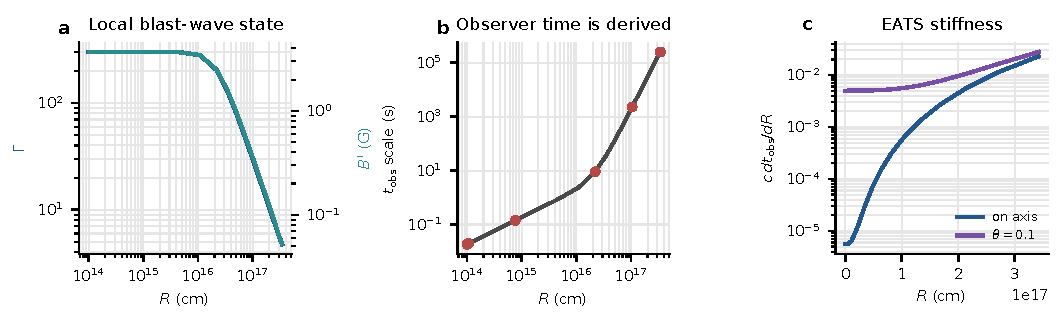
\includegraphics[width=\textwidth]{figures/fig1_radius_state.pdf}
  \caption{
\gptareaderanchor{gpta-seg-000007}%
\asgard\ 计算的半径排序状态。(a) 公共输入被归一化为固定序列：运行时配置、动力学、电子和光子状态、有界可选分支以及观测者投影。(b) 在形成观测产物之前，冲击波洛伦兹因子和共动磁场被存储在激波半径网格上。(c) 等到达时间映射使用 \(t_{\rm obs}=(1+z)[t_{\rm on}(R)+R(1-\mu)/c]\)，因此不同的角度单元将相同的本地半径序列映射到不同的观测时间序列。}
  \label{fig:radius-state}
\end{figure*}


\gptareaderanchor{gpta-seg-000008}%
支持的观测者产品来源于此状态记录：多频通量、固定时间谱、波段积分通量、曝光平均通量、成分分辨通量以及诊断状态轨迹。成分记录包含总通量和活跃的物理通道：正向激波同步辐射和SSC辐射、反向激波同步辐射和SSC辐射、跨区逆康普顿辐射、强子同步辐射、对同步辐射以及中微子输出。诊断状态揭示了半径、洛伦兹因子、磁场、电子谱、\(\chi\)分辨电子场、强子种类、光子存活因子、反向激波状态以及（当这些计算激活时）次级反向激波事件诊断。

\begin{figure*}[!tp]
  \centering
  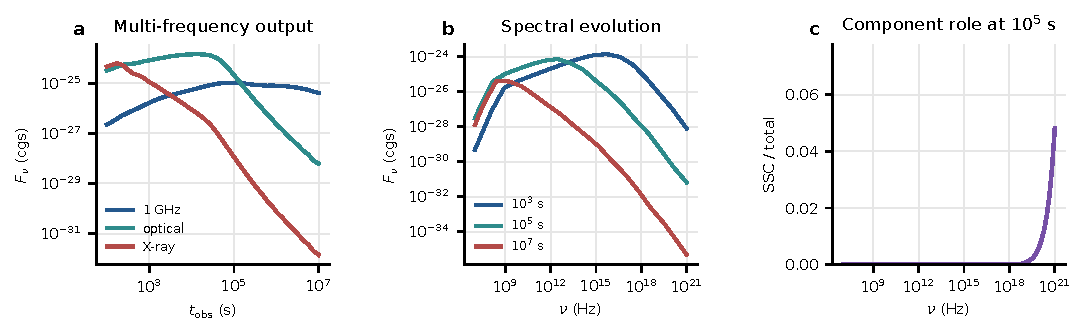
\includegraphics[width=\textwidth]{figures/fig2_forward_api.pdf}
  \caption{
\gptareaderanchor{gpta-seg-000009}%
在一次正向激波计算中从动力学到观测者产物。(a) 局部的\(\Gamma(R)\)和\(B'(R)\)状态为观测者计算提供源项。(b) 多频光变曲线、(c) 固定时间谱和(d) SSC通量分数由同一半径排序状态组合而成。该图是一个核算诊断，并非对特定暴发的独立拟合。}
  \label{fig:forward-api}
\end{figure*}


\gptareaderanchor{gpta-seg-000010}%
公共模型定义被有意地限制。\asgard\ 并非作为更快速的光变曲线专用工具的替代品而提出。它在本文中的目的是通过保留观察者投影之前的状态，使耦合的余辉计算可被检查。支持的运行时族列在Section~\ref{sec:limits}中；这些族之外的物理组合不被解释为建模行为。

\section{动力学与喷流/介质设置} \label{sec:dynamics}


\gptareaderanchor{gpta-seg-000011}%
动力学部分定义了在计算任何辐射之前的激波。前向激波首先需要外部密度\(n(R)\)、角能量分布和角洛伦兹因子分布。根据这些输入，动力学模块写出\(\Gamma(R)\)、扫过的物质、内能以及粒子和辐射模块所用的磁场。

\subsection{外部介质}


\gptareaderanchor{gpta-seg-000012}%
外部介质是被前向激波扫过的气体。在动力学中，它通过质子数密度\(n(R)\)进入。\asgard{}支持三种类型：均匀介质、Chevalier–Li \(k=2\)星风以及表格化的径向轮廓。相同的\(n(R)\)随后被传递给该半径处的粒子注入、光子产生、吸收以及观测者投影。

\subsubsection{解析介质}


\gptareaderanchor{gpta-seg-000013}%
分析介质直接给出了上游密度。均匀介质具有恒定密度，而恒星风则按\(R^{-2}\)衰减。所实现的形式为
\begin{equation}
\begin{aligned}
n(R) &= n_{\rm ISM},\\
n_{\rm w}(R) &= \frac{A_\ast A_0}{m_pR^2},\\
n_0(R) &=
\begin{cases}
n_{\rm ISM}, & n_{\rm w}(R)\le n_{\rm ISM}/\eta_{\rm w},\\
n_{\rm w}(R), & n_{\rm w}(R)> n_{\rm ISM}/\eta_{\rm w},
\end{cases}\\
R_0 &= \left(\frac{A_\ast A_0}{m_p n_{\rm cap}}\right)^{1/2}.
\end{aligned}
\end{equation}

\gptareaderanchor{gpta-seg-000014}%
这里\(n_{\rm ISM}\)是均匀密度，\(A_0\)是Chevalier--Li风质量加载尺度，\(m_p\)是质子质量，而\(\eta_{\rm w}\)设定风与星际介质之间的转换\citep{ChevalierLi2000}。如果用户提供上限密度\(n_{\rm cap}\)，代码将定义\(R_0\)，并在该半径内将风密度保持为\(n_{\rm w}(R_0)\)。均匀介质保持为\(n_{\rm ISM}\)。该上限是一个刚性内部密度状态；不支持\(k\ne2\)的风剖面。

\subsubsection{表格化介质与跃变}


\gptareaderanchor{gpta-seg-000015}%
表格化的介质从用户点提供上游密度。表格包含正半径 \(R_i\) 和正密度 \(n_i\)，半径严格递增且 \(N_\rho\le N_{\rho,\max}\)。在两个相邻点之间，代码使用局部幂律。
\begin{equation}
\begin{aligned}
n(R) &=
\exp\left[
\operatorname{interp}\left(\ln R;\,\ln R_i,\,\ln n_i\right)
\right],\\
n(R) &=
n_i
\left(\frac{R}{R_i}\right)^{q_i},\qquad
q_i\equiv\frac{\ln(n_{i+1}/n_i)}{\ln(R_{i+1}/R_i)} .
\end{aligned}
\end{equation}

\gptareaderanchor{gpta-seg-000016}%
前两个表格点设置了表格下方的外推，后两个设置了表格上方的外推。因此，该表格在两端均按幂律进行扩展。表格化介质和高斯跳跃模型是独立的输入系列；它们不会在一次运行中合并。

密度跳跃是解析基线密度的局部扰动。它们仅用于解析介质系列。对于几个高斯结构，密度是
\begin{equation}
n(R)=n_0(R)
\left[
1+\sum_j
(f_j-1)
\exp\left(
-\frac{(R-R_j)^2}{2(\Delta R_j)^2}
\right)
\right].
\end{equation}

\gptareaderanchor{gpta-seg-000017}%
这里 \(R_j\) 是中心位置，\(f_j\) 是密度因子，而 \(\Delta R_j\equiv w_jR_j\) 为宽度。单个高斯分布对应较早期的单跳变界面。当 \(f_j<1\) 时表示密度低谷，且仅在总密度保持正值时才允许出现。这些高斯分布是用于余辉计算的受控密度扰动；本文并不声称每个高斯分布对应唯一的环境 \citep{DaiLu2002,NakarGranot2007,UhmZhang2014}。

介质设置还定义了严格的输入边界。它支持 \(N_J\le N_{J,\max}\) 个高斯结构或 \(N_\rho\le N_{\rho,\max}\) 个表格数据点。它拒绝非正的跳跃半径、因子或宽度；非正的表格半径或密度；点数少于两个的表格；以及半径未按序排列的表格。这些检查界定了所支持的介质族，而非额外的物理假设。

\subsection{喷流角向轮廓}


\gptareaderanchor{gpta-seg-000018}%
喷流轮廓设定了每个极向元素的初始能量和洛伦兹因子。这是一个初始条件，而非角度演化模型。一个平顶喷流在\(\theta_j\)内部是均匀的，外部则为空：
\begin{equation}
\begin{aligned}
E_{\rm iso}(\theta) &=
\begin{cases}
E_c, & \theta<\theta_j,\\
0, & \theta\ge\theta_j,
\end{cases}\\
\Gamma_0(\theta) &=
\begin{cases}
\Gamma_c, & \theta<\theta_j,\\
1, & \theta\ge\theta_j .
\end{cases}
\end{aligned}
\end{equation}

\gptareaderanchor{gpta-seg-000019}%
高斯喷流会使各向同性等效能量和\(\Gamma_0-1\)随着离轴距离的增加而减小：
\begin{equation}
\begin{aligned}
E_{\rm iso}(\theta) &=
E_c\exp\left[-\frac{\theta^2}{2\theta_c^2}\right],\\
\Gamma_0(\theta) &=
1+(\Gamma_c-1)\exp\left[-\frac{\theta^2}{2\theta_c^2}\right],
\end{aligned}
\end{equation}

\gptareaderanchor{gpta-seg-000020}%
高斯轮廓仅在声明的外部支撑\(\theta_{\max}\)内部使用。幂律喷流具有平坦核心和幂律翼部：
\begin{equation}
\begin{aligned}
E_{\rm iso}(\theta) &=
E_c
\begin{cases}
1, & \theta\le \theta_c,\\
(\theta/\theta_c)^{-k_E}, & \theta>\theta_c,
\end{cases}\\
\Gamma_0(\theta) &=
\begin{cases}
\Gamma_c, & \theta\le \theta_c,\\
1+(\Gamma_c-1)(\theta/\theta_c)^{-k_\Gamma}, & \theta>\theta_c .
\end{cases}
\end{aligned}
\end{equation}

\gptareaderanchor{gpta-seg-000021}%
这里 \(E_c\) 和 \(\Gamma_c\) 是轴上值，\(\theta_c\) 是核心角，\(k_E\) 和 \(k_\Gamma\) 设定翼斜率。公共轮廓默认使用 \(k_\Gamma=k_E\)，除非提供了独立的洛伦兹因子斜率。这些轮廓提供独立的角元素；当前后端不演化横向扩展。

\subsection{前向激波动力学变量}


\gptareaderanchor{gpta-seg-000022}%
前向激波状态携带了后续辐射模块所需的变量。状态向量是
\begin{equation}
\mathbf{y}=(\Gamma,\mathcal{M},U,R),
\end{equation}

\gptareaderanchor{gpta-seg-000023}%
且自变量为源帧同轴到达坐标
\(t_{\rm on}\)。其中\(\Gamma\)为爆炸波洛伦兹因子，\(U\)为内能，\(R\)为激波半径。第二项\(\mathcal{M}\)依赖于动力学分支：分支1和2存储扫过的数量列，而分支3存储扫过的质量。该向量是电子注入和辐射的局部动力学输入。

坐标\(t_{\rm on}\)追踪同轴光子的到达时间，而非实验室时间。沿径向序列，
\begin{equation}
\begin{aligned}
\frac{dt_{\rm on}}{dR} &= \frac{1-\beta}{\beta c},\\
\frac{dR}{dt_{\rm on}} &= \frac{\beta c}{1-\beta},\\
\beta &= \sqrt{1-\Gamma^{-2}}.
\end{aligned}
\end{equation}

\gptareaderanchor{gpta-seg-000024}%
第二个关系因此不是实验室参考系中的激波速度。而是当\(t_{\rm on}\)为独立变量时，半径网格被遍历的速率。离轴观测者时间随后通过\(t_{\rm obs}=(1+z)[t_{\rm on}(R)+R(1-\mu)/c]\)组合得到，因此该坐标是一个动力学排序变量，而非最终的观测时钟。

磁场由局域的后激波能量密度决定。对于前向激波，代码使用
\begin{equation}
\begin{aligned}
e' &\simeq4(\Gamma^2-1)n(R)m_pc^2,\\
B' &=\left(8\pi\epsilon_B e'\right)^{1/2}
=\left[32\pi\epsilon_B n(R)m_pc^2(\Gamma^2-1)\right]^{1/2}.
\end{aligned}
\end{equation}

\gptareaderanchor{gpta-seg-000025}%
这里\(n(R)\)是上游质子密度，\(\epsilon_B\)是磁能分数。输出\(B'(R)\)决定了同步辐射冷却、同步辐射发射、SSC种子产生以及磁诊断。

动力学分支还记录了用于启动和诊断的电子能量尺度。以\(t'_{\rm dyn}\equiv\Gamma t_{\rm on}\)表示，这些尺度为
\begin{equation}
\begin{aligned}
\gamma_c=
\frac{6\pi m_ec}{\sigma_{\rm es} B'^2t'_{\rm dyn}},
\\
\gamma_m=
1+\frac{\epsilon_e}{f_e}
\frac{m_p}{m_e}
\frac{p-2}{p-1}
(\Gamma-1).
\end{aligned}
\end{equation}

\gptareaderanchor{gpta-seg-000026}%
这里\(\gamma_c\)是同步加速冷却洛伦兹因子，\(\gamma_m\)是注入非热电子的最小洛伦兹因子，\(\epsilon_e\)是电子能量分数，\(f_e\)是加速电子分数，\(p\)是注入电子指数。如果\(\gamma_c>\gamma_m\)且\(p\ge2\)，动力学子分支将辐射分数估计为
\begin{equation}
\epsilon_{\rm eff}=\epsilon_e\left(\frac{\gamma_m}{\gamma_c}\right)^{p-2};
\end{equation}

\gptareaderanchor{gpta-seg-000027}%
否则，它使用 \(\epsilon_{\rm eff}=\epsilon_e\)。该估计仅影响需要辐射效率的动力学分支；电子传输模块仍显式演化 \(N_e\)。

第一个径向网格需要一个减速尺度。该设置首先定义
\begin{equation}
\mathcal{D}_0=
\frac{E_{\rm iso}}{4\pi(\Gamma_0-1)m_pc^2},
\end{equation}

\gptareaderanchor{gpta-seg-000028}%
其中\(E_{\rm iso}\)和\(\Gamma_0\)分别是角度元素的初始各向同性等效能量和洛伦兹因子。减速半径的分析估计是
\begin{equation}
\begin{aligned}
R_{\rm dec,ISM}
&=\left(\frac{n_{\rm ISM}\Gamma_0}{\mathcal{D}_0}\right)^{-1/3},\\
R_{\rm dec,wind}
&=\frac{3\mathcal{D}_0}{2(A_\ast A_0/m_p)\Gamma_0}.
\end{aligned}
\end{equation}

\gptareaderanchor{gpta-seg-000029}%
这里 \(A_\ast A_0/m_p\) 是风数密度归一化。对于风介质，设置使用 \(R_{\rm dec}=\min(R_{\rm dec,ISM},R_{\rm dec,wind})\)；否则使用 \(R_{\rm dec}=R_{\rm dec,ISM}\)。相应的轴向到达尺度为
\[
t_{\rm dec}=\frac{R_{\rm dec}(1-\beta_0)}{\beta_0c},
\qquad
\beta_0=(1-\Gamma_0^{-2})^{1/2}.
\]

\gptareaderanchor{gpta-seg-000030}%
当 \(\Gamma_0\gg1\) 时，这简化为 \(t_{\rm dec}\simeq R_{\rm dec}/(2\Gamma_0^2c)\)。求解器利用这一尺度在从惯性滑行到减速过渡的区域布置早期径向点；它不强行采用分段幂律。

\subsection{动力学分支}


\gptareaderanchor{gpta-seg-000031}%
动力学模块提供了三种演化同一正向激波状态的方式。分支1是余辉计算中常用的辐射效率形式\citep{BlandfordMcKee1976,HuangDaiLu1999}。分支2是一种遗留的可变指数形式。分支3是默认的质量-能量基线。所有三个分支都输出\(\Gamma(R)\)、扫过物质、\(U(R)\)和\(R\)；它们在惯性项和能量预算的写法上有所不同。

\subsubsection{共享状态方程与注入源}


\gptareaderanchor{gpta-seg-000032}%
状态方程决定了受激气体如何储存热量。分支2和3需要一个从相对论极限变化到牛顿极限的绝热指数。\asgard\ 评估一个固定的状态方程拟合：
\begin{equation}
\begin{aligned}
u&=\Gamma\beta,\qquad
\Theta=\frac{u}{3}\frac{u+a_\Theta u^2}{1+u+a_\Theta u^2},\\
\zeta&=\frac{\Theta}{a_\zeta+\Theta},\qquad
\hat{\gamma}=
\frac{1}{3}\sum_{r=0}^{N_{\hat\gamma}}a_r\zeta^r .
\end{aligned}
\end{equation}

\gptareaderanchor{gpta-seg-000033}%
此处 \(u\) 是无量纲的四速度，\(\Theta\) 是类似温度的拟合变量，\(\zeta\) 将该变量映射到多项式域。系数 \((a_\Theta,a_\zeta,\{a_r\})\) 和阶数 \(N_{\hat\gamma}\) 由相对论性麦克斯韦-于特纳状态方程拟合 \citep{Service1986,Peer2012} 确定。输出为 \(\hat{\gamma}(\Gamma)\)，并非针对任何光变曲线的拟合。

能量注入源是往动力学中添加的一个预设光度。在源参考系时间中，它
\begin{equation}
\mathcal{L}(t_{\rm on})=
\begin{cases}
L_0(t_{\rm on}/t_1)^{q}, & t_1\le t_{\rm on}\le t_2,\\
0, & \text{otherwise},
\end{cases}
\end{equation}

\gptareaderanchor{gpta-seg-000034}%
其中\(t_1\)和\(t_2\)是源参考系中的注入边界，\(L_0\)是光度归一化常数，\(q\)是时间指数。公共构造函数以观测者参考系形式存储边界，动力学过程在评估源参考系方程前将其除以\(1+z\)。该项改变爆炸波能量预算；它并非独立的自旋下降计算。

所选的动力学分支定义了能量注入的作用位置。分支1和分支3在洛伦兹因子方程中包含\(\mathcal{L}(t_{\rm on})\)。分支2不包含该源项。因此，能量注入是局部动力学的一部分，而非对最终光变曲线的修正。

\subsubsection{扫掠介质状态变量}


\gptareaderanchor{gpta-seg-000035}%
扫过介质变量记录了进入激波区的外部气体量。分支1和2演化出扫过数柱\(\mu\)。分支3演化出物理扫过质量\(M\)。它们遵循
\begin{equation}
\begin{aligned}
q_\mu &\equiv\frac{d\mu}{dt_{\rm on}}
=n(R)R^2\frac{dR}{dt_{\rm on}},\\
\frac{dM}{dR} &=4\pi n(R)R^2m_p .
\end{aligned}
\end{equation}

\gptareaderanchor{gpta-seg-000036}%
相应的初始喷射物归一化是
\begin{equation}
\begin{aligned}
\mu_0 &=\frac{E_{\rm iso}}{4\pi(\Gamma_0-1)m_pc^2},\\
M_0 &=\frac{E_{\rm iso}}{(\Gamma_0-1)c^2}.
\end{aligned}
\end{equation}

\gptareaderanchor{gpta-seg-000037}%
对于分支1和2，报告的扫掠质量为 \(M_{\rm sw}=4\pi m_p\mu\)。在分支3中，\(M\) 已经是以克为单位的扫掠质量，并且
\[
\frac{dM}{dt_{\rm on}}=\frac{dM}{dR}\frac{dR}{dt_{\rm on}}.
\]

\subsubsection{分支1：辐射效率动力学}


\gptareaderanchor{gpta-seg-000038}%
分支1通过平衡扫过的减速与可选的能量注入来演化\(\Gamma\)。其方程为
\begin{equation}
\begin{aligned}
\frac{d\Gamma}{dt_{\rm on}}=
\frac{-(\Gamma^2-1)q_\mu
+\mathcal{L}(t_{\rm on})/(4\pi m_pc^2)}
{\mu_0+\epsilon_{\rm eff}\mu
+2(1-\epsilon_{\rm eff})\Gamma\mu},
\\
\frac{dU}{dt_{\rm on}}=(\Gamma-1)q_\mu .
\end{aligned}
\end{equation}

\gptareaderanchor{gpta-seg-000039}%
\(d\Gamma/dt_{\rm on}\)中的负项是由扫过物质引起的减速。正项是可选的注入光度。分支在同一扫过柱状态\(\mu\)上输出\(\Gamma\)和\(U\)。

\subsubsection{分支2：可变指数遗留动力学}


\gptareaderanchor{gpta-seg-000040}%
分支2保持扫过的柱\(\mu\)，但让\(\hat{\gamma}\)改变有效惯性。定义
\begin{equation}
\begin{aligned}
\mathcal{N}_2&=
\hat{\gamma}(\Gamma^2-1)-(\hat{\gamma}-1)\Gamma\beta^2,
\\
\mathcal{D}_2&=\mu_0+\epsilon_{\rm eff}\mu\\
&\quad
+(1-\epsilon_{\rm eff})\mu
\left[
2\hat{\gamma}\Gamma-(\hat{\gamma}-1)(1+\Gamma^{-2})
\right],
\\
\frac{d\Gamma}{dt_{\rm on}}&=-
\frac{\mathcal{N}_2}{\mathcal{D}_2}
q_\mu,\\
\frac{dU}{dt_{\rm on}}&=(\Gamma-1)q_\mu .
\end{aligned}
\end{equation}

\gptareaderanchor{gpta-seg-000041}%
分支2是用于动力学比较的可选遗留选项。它不是出版图表的默认分支。

\subsubsection{分支3：质量--能量基线}


\gptareaderanchor{gpta-seg-000042}%
分支3使用物理扫过的质量\(M\)。这使得质量和能量收支更加明确。定义。
\begin{equation}
\begin{aligned}
X &= \Gamma^2-1,\\
\frac{dM}{dt_{\rm on}} &= \frac{dM}{dR}\frac{dR}{dt_{\rm on}},
\end{aligned}
\end{equation}

\gptareaderanchor{gpta-seg-000043}%
其中\(X\)是相对论动能因子的简称。洛伦兹因子方程为
\begin{equation}
\begin{aligned}
\mathcal{N}_3&=
-\frac{dM}{dR}c^2\Gamma X
(\hat{\gamma}\Gamma-\hat{\gamma}+1)
\\
&\quad
-(\hat{\gamma}X+1)\Gamma(1-\hat{\gamma})
\frac{3U}{R}
+\Gamma^2\mathcal{L}(t_{\rm on})
\left(\frac{dR}{dt_{\rm on}}\right)^{-1},
\\
\mathcal{D}_3&=
\Gamma^2(M_0+M)c^2
+(\hat{\gamma}^2X+3\hat{\gamma}-2)U .
\end{aligned}
\end{equation}
\begin{equation}
\frac{d\Gamma}{dt_{\rm on}}=
\frac{\mathcal{N}_3}{\mathcal{D}_3}\frac{dR}{dt_{\rm on}}.
\end{equation}

\gptareaderanchor{gpta-seg-000044}%
\(\mathcal{N}_3\)中的三项具有直接的含义。第一项是新扫掠质量的惯性，第二项是膨胀激波气体所做的功，第三项是可选的注入光度。这些项使得第三分支成为正向激波计算的默认状态。

内能因激波加热、绝热膨胀以及可选的能量注入而发生变化。径向膨胀和加热项为
\begin{equation}
\begin{aligned}
\mathcal{E}_R &=
\frac{3}{R}
-\frac{1}{\Gamma}
\left(\frac{dR}{dt_{\rm on}}\right)^{-1}
\frac{d\Gamma}{dt_{\rm on}},\\
\mathcal{H}_R &=(1-\epsilon_{\rm eff})(\Gamma-1)
\frac{dM}{dR}c^2 .
\end{aligned}
\end{equation}
能量方程为
\begin{equation}
\frac{dU}{dt_{\rm on}}=
\left[\mathcal{H}_R-(\hat{\gamma}-1)\mathcal{E}_R U\right]
\frac{dR}{dt_{\rm on}}
+\mathcal{L}(t_{\rm on}).
\end{equation}

\gptareaderanchor{gpta-seg-000045}%
这个方程描述了局部热预算，它随后决定了电子注入和磁场。

\subsection{前向动力学积分}


\gptareaderanchor{gpta-seg-000046}%
前向动力学积分器将分支方程转化为存储的径向状态。它读取公共模型，固定密度分布，并进行积分。
\begin{equation}
\mathbf{y}=(\Gamma,Y_2,U,R)
\end{equation}

\gptareaderanchor{gpta-seg-000047}%
在 \(t_{\rm on}\) 网格上。条目 \(Y_2\) 对于分支1和2是 \(\mu\)，对于分支3是 \(M\)。在每个被接受的步之后，公共数组是
\begin{equation}
\begin{aligned}
t_{{\rm obs},i}&=(1+z)t_{{\rm on},i},\\
\Gamma_i&=Y_{\Gamma,i},\qquad R_i=Y_{R,i},\\
M_{{\rm sw},i}&=
\begin{cases}
4\pi m_pY_{2,i},
& \text{branches 1 and 2},\\
Y_{2,i},
& \text{branch 3}.
\end{cases}
\end{aligned}
\end{equation}

\gptareaderanchor{gpta-seg-000048}%
这些数组是电子、光子、反向激波、强子以及观测模块读取的动态输出。运行时容器和网格启动细节详见附录~\ref{app:projection-runtime}。

数值更新采用四阶龙格-库塔步长。对于 \(t_{{\rm on},i-1}>0\)，积分器将变量从 \(t_{\rm on}\) 变换为
\begin{equation}
\begin{aligned}
s=\ln(t_{\rm on}/t_{{\rm on},i-1}),
\frac{d\mathbf{y}}{ds}
=t_{\rm on}\frac{d\mathbf{y}}{dt_{\rm on}}
=t_{\rm on}F(t_{\rm on},\mathbf{y}).
\end{aligned}
\end{equation}

\gptareaderanchor{gpta-seg-000049}%
这里\(F\equiv d\mathbf{y}/dt_{\rm on}\)是选定的动力学分支。第一个区间，其中\(t_{{\rm on},i-1}=0\)，直接在线性\(t_{\rm on}\)中推进。此更新保留了后续模块所使用的半径有序状态。

自适应检查比较同一区间的两次积分。令\(\mathbf{y}^{\rm f}\)为当前的\(m\)子步试验解，\(\mathbf{y}^{\rm c}\)为之前的\(m/2\)子步比较解。正状态项上的相对误差为
\begin{equation}
\epsilon_{\rm RK}^\ast=
\max_{a\in\mathcal{I}_y}
\frac{2|y_a^{\rm f}-y_a^{\rm c}|}
{y_a^{\rm f}+y_a^{\rm c}},
\qquad
\mathcal{I}_y\equiv\{a\,|\,y_a^{\rm f}+y_a^{\rm c}>0\}.
\end{equation}

\gptareaderanchor{gpta-seg-000050}%
细分持续进行，直到 \(\epsilon_{\rm RK}^\ast<\epsilon_{\rm RK}\)。每次试验还必须保持 \(\Gamma>1\)。容差 \(\epsilon_{\rm RK}\) 是固定的RK精度阈值。这些检查定义了积分器所使用的相对论性激波状态域。在此域之外的试验不被接受为半径步长。

\subsection{Python 绑定边界}


\gptareaderanchor{gpta-seg-000051}%
Python动力学命名空间仅是一个绑定层。它将编译好的前向和反向动力学内核暴露给更高级别的编排。它不添加爆震波方程、激波跳跃条件或积分步骤。物理方程是上述编译好的前向动力学以及第\ref{sec:reverse-shock}节中的反向激波方程。

\section{粒子与辐射输运} \label{sec:electron}


\gptareaderanchor{gpta-seg-000052}%
粒子与辐射层紧随产生余辉光谱的物质之后。在每个半径处，激波注入非热电子。这些电子通过同步辐射、逆康普顿散射和绝热冷却损失能量，其辐射构建了用于同步自康普顿散射、吸收及可选反馈分支的光子场。一维求解器返回\(N_e(\gamma,R)\)、同步辐射光度、种子光子密度以及截止频率\(\nu_m\)、\(\nu_c\)和\(\nu_a\)。二维路径增加了下游\(\chi\)分辨的电子场和光子场。求解器的选择改变离散化方式，而非物理注入律\citep{LeVeque2002,JiangShu1996,HesthavenWarburton2008}。

\subsection{共享电子状态、源项与坐标}

\subsubsection{命名空间边界}


\gptareaderanchor{gpta-seg-000053}%
Python电子命名空间仅是一个绑定层。它选择一个编译好的电子模块，并将其暴露给公共API。它不添加注入律、冷却项、发射率公式或输运方程。不受支持的历史名称直接缺失，而非重定向到另一个求解器。

\subsubsection{连续状态与求解器存储}


\gptareaderanchor{gpta-seg-000054}%
前向电子态在激波向外传播时演化电子能谱。所有前向电子求解器均基于相同的连续性方程，其中半径作为自变量。
\begin{equation}
\frac{\partial N_e}{\partial R}
+\frac{\partial}{\partial\gamma}
\left(g_RN_e\right)
=Q_e+Q_e^{\rm sec},
\end{equation}

\gptareaderanchor{gpta-seg-000055}%
其中 \(N_e(\gamma,R)\) 表示微分电子数密度，
\(g_R=d\gamma/dR\)，而 \(Q_e\) 是主要的激波源。漂移项 \(g_R\)
包含辐射冷却和绝热冷却。在独立的轻子计算中，次级源
\(Q_e^{\rm sec}\) 为零。只有当强子反馈分支将Bethe-Heitler、\(pp\) 或
\(\gamma\gamma\) 次级粒子反馈回电子方程时，它才会被提供。

默认的隐式求解器将谱存储在自然对数能量网格上。
对于 \(x=\ln\gamma\)，网格密度为
\begin{equation}
N_x\equiv\frac{dN_e}{dx}=\gamma N_e,
\qquad x=\ln\gamma .
\end{equation}

\gptareaderanchor{gpta-seg-000056}%
这是每个\(x\)区间的物理密度。由于\(x\)是自然对数，因此不会出现\(\ln 10\)雅可比行列式。某些核函数将相同的粒子存储在对数四速度坐标中。当初始条件和源投影到该存储网格时，会应用坐标雅可比行列式。代表性的隐式壳更新为
\begin{equation}
\left(\mathbf{I}-\mathbf{A}_i\right)\mathbf{N}_{i+1}
=\mathbf{N}_{i}+\Delta R_i\,\mathbf{Q}_{i},
\end{equation}

\gptareaderanchor{gpta-seg-000057}%
其中矩阵\(\mathbf{A}_i\)由面漂移系数组装而成。从高能到低能的扫描步骤求解隐式部分。源项在单元边界上积分，因此更新过程演化的是单元平均值，而非点样本。

\subsubsection{有限壳层源与注入标度}


\gptareaderanchor{gpta-seg-000058}%
电子注入采用与动力学相同的密度\(n(R)\)。未引入独立的电子密度定律。壳层体积为
\begin{equation}
V(R)=\frac{4\pi R^3}{3}.
\end{equation}

\gptareaderanchor{gpta-seg-000059}%
第一个活动半径之前的被扫过电子数量是
\begin{equation}
N_{\rm init}=\int_0^{R_{\rm ini}}4\pi R^2 n(R)\,dR .
\end{equation}

\gptareaderanchor{gpta-seg-000060}%
因此，对于均匀分支，有 \(N_{\rm init}=n_{\rm ISM}V(R_{\rm ini})\)。对于解析风和有顶风分支，相同的积分在 \(n(R)\) 对应的分段区间上进行计算。从 \(R_s\) 开始的有限壳层贡献了径向源。
\begin{equation}
q_R(R_s,\Delta R)
\equiv
n(R_s)\frac{V(R_s+\Delta R)-V(R_s)}{\Delta R}.
\end{equation}

\gptareaderanchor{gpta-seg-000061}%
这是在有限壳层上评估的每单位半径扫过的上游粒子数量。乘以网格宽度即可得到该壳层注入的粒子数。

注入能量范围由最小和最大电子洛伦兹因子设定。最大加速能量由加速与同步辐射损失之间的平衡得出：
\begin{equation}
\gamma_{\max}=\frac{3m_ec^2}{\left(8e^3B'\right)^{1/2}} .
\end{equation}

\gptareaderanchor{gpta-seg-000062}%
源在 \(\gamma_{\max}\) 以下没有被截断。在 \(\gamma_{\max}\) 以上，它是指数抑制的：
\begin{equation}
\mathcal{C}_{\max}(\gamma)=
\begin{cases}
1, & \gamma\le\gamma_{\max},\\
\exp(1-\gamma/\gamma_{\max}), & \gamma>\gamma_{\max}.
\end{cases}
\end{equation}


\gptareaderanchor{gpta-seg-000063}%
注入最小值取决于电子指数 \(p\)。对于 \(p>2\)，
\begin{equation}
\gamma_m=1+\frac{p-2}{p-1}
\frac{\epsilon_e}{f_e}
\frac{m_p}{m_e}(\Gamma-1).
\end{equation}
对于 \(1<p<2\)，
\begin{equation}
\gamma_m=
\left[
\frac{2-p}{p-1}
\frac{\epsilon_e}{f_e}\frac{m_p}{m_e}(\Gamma-1)
\gamma_{\max}^{p-2}
\right]^{1/(p-1)}+1.
\end{equation}

\gptareaderanchor{gpta-seg-000064}%
对于 \(p=2\)，归一化是对数形式的：
\begin{equation}
\gamma_m\ln\left(\frac{\gamma_{\max}}{\gamma_m}\right)
=\frac{\epsilon_e}{f_e}\frac{m_p}{m_e}(\Gamma-1).
\end{equation}

\gptareaderanchor{gpta-seg-000065}%
因此，所实现的注入模型对 \(p\) 使用了正确的分支；它不会在 \(p>2\) 表达式的定义域之外应用该表达式。

前向激波源是一个幂律分布，并带有上述高能截断。在活性支撑上的归一化是
\begin{equation}
a_p=f_e\frac{1-p}{\gamma_{\max}^{1-p}-\gamma_m^{1-p}} .
\end{equation}

\gptareaderanchor{gpta-seg-000066}%
局部源振幅为 \(A_R\equiv q_R(R_s,\Delta R)a_p\)。在自然对数伽马细胞中，源形状为
\begin{equation}
\begin{aligned}
S_x(x)
&=\exp[(1-p)x]
\mathcal{C}_{\max}[\exp(x)]H[\exp(x)-\gamma_m],\\
Q_{x,j}
&=A_R\,\mathcal I_{x,j},\\
\mathcal I_{x,j}
&=\frac{1}{\Delta x_j}
\int_{x_{j-1/2}}^{x_{j+1/2}}
S_x(x)\,dx .
\end{aligned}
\end{equation}

\gptareaderanchor{gpta-seg-000067}%
这里\(H\)是Heaviside函数。输出量\(Q_{x,j}\)是电子传输求解器使用的注入的单元平均源。

\subsubsection{共享网格上的初始谱}


\gptareaderanchor{gpta-seg-000068}%
初始电子谱被放置在自然对数能量网格上。网格点为
\begin{equation}
\Delta_g\equiv \frac{\ln(\gamma_H/\gamma_L)}{N_\gamma-1},
\qquad
\gamma_i=\gamma_L\exp[(i-1)\Delta_g],
\end{equation}

\gptareaderanchor{gpta-seg-000069}%
其中\(\gamma_L\)和\(\gamma_H\)是固定的网格边界，而\(\gamma_H\)选自初始加速度截止值。所有求解器均从相同的物理谱开始；仅存储坐标可以改变。

对于幂律段，转换为对数伽马密度
\begin{equation}
\begin{aligned}
\frac{dN_e}{d\gamma}
&=A\gamma^{-s}\mathcal{C}_{\max}(\gamma),\\
\frac{dN_e}{dx}=A\gamma^{1-s}\mathcal{C}_{\max}(\gamma),
x&=\ln\gamma .
\end{aligned}
\end{equation}

\gptareaderanchor{gpta-seg-000070}%
初始谱取决于 \(\gamma_c\) 和 \(\gamma_m\) 的顺序。设 \(N_0\equiv N_{\rm init}\)。在快冷却情况下，\(\gamma_c<\gamma_m\)，谱为
\begin{equation}
\begin{gathered}
A_{\rm f}\equiv N_0\gamma_c,\\
\frac{dN_e}{d\gamma}=
\begin{cases}
A_{\rm f}\gamma^{-2}\mathcal{C}_{\max}(\gamma),
& \gamma_c\le\gamma<\gamma_m,\\
A_{\rm f}\gamma_m^{p-1}\gamma^{-p-1}
\mathcal{C}_{\max}(\gamma),
& \gamma\ge\gamma_m,\\
0, & \text{otherwise}.
\end{cases}
\end{gathered}
\end{equation}

\gptareaderanchor{gpta-seg-000071}%
在慢冷却情况下，\(\gamma_m\le\gamma_c\)，频谱是
\begin{equation}
\begin{gathered}
A_{\rm s}\equiv N_0(p-1)\gamma_m^{p-1},\\
\frac{dN_e}{d\gamma}=
\begin{cases}
A_{\rm s}\gamma^{-p}
\mathcal{C}_{\max}(\gamma),
& \gamma_m\le\gamma<\gamma_c,\\
A_{\rm s}\gamma_c\gamma^{-p-1}
\mathcal{C}_{\max}(\gamma),
& \gamma\ge\gamma_c,\\
0, & \text{otherwise}.
\end{cases}
\end{gathered}
\end{equation}

\gptareaderanchor{gpta-seg-000072}%
点值求解器在\(\gamma_i\)处对这些谱进行采样。而守恒求解器则存储单元平均值：
\begin{equation}
N_{x,j}^{\rm init}=\frac{1}{\Delta x_j}
\int_{x_{j-1/2}}^{x_{j+1/2}}
\frac{dN_e}{dx}\,dx .
\end{equation}

\gptareaderanchor{gpta-seg-000073}%
将积分在\(\gamma_m\)、\(\gamma_c\)和\(\gamma_{\max}\)处分割。如果求解器存储不同的坐标，则相同的物理谱仅通过坐标雅可比矩阵进行变换。求积和坐标映射公式见附录~\ref{app:electron-solvers}。

\subsubsection{壳层源的坐标投影}


\gptareaderanchor{gpta-seg-000074}%
前向激波源被投影到求解器存储的任何坐标中。只有坐标度量发生变化。在一般存储坐标\(y\)中，单元源是
\begin{equation}
\begin{aligned}
S_y(y)&=S_x[x(y)]\,\frac{dx}{dy},\\
Q_{y,j}
&=A_R\,\mathcal I_{y,j},\\
\mathcal I_{y,j}
&=\frac{1}{\Delta y_j}
\int_{y_{j-1/2}}^{y_{j+1/2}}
S_y(y)\,dy .
\end{aligned}
\end{equation}

\gptareaderanchor{gpta-seg-000075}%
因此，每个求解器都会接收到相同的注入物理分布，即使它以不同坐标存储该分布。

\subsubsection{反向激波动能源}


\gptareaderanchor{gpta-seg-000076}%
反向激波电子使用动能幂律。这与前向激波源不同，后者表示为 \(\gamma\) 的幂律。反向激波源的活跃部分由
\begin{equation}
I_m(\gamma)=
\begin{cases}
1, & \gamma>\gamma_m,\\
0, & \gamma\le\gamma_m .
\end{cases}
\end{equation}

\gptareaderanchor{gpta-seg-000077}%
在对数-伽马坐标中，非归一化密度为
\begin{equation}
\Psi_x(\gamma)=\gamma(\gamma-1)^{-p}
\mathcal{C}_{\max}(\gamma)I_m(\gamma).
\end{equation}

\gptareaderanchor{gpta-seg-000078}%
然后，将单元格平均值 \(\bar\Psi_{x,j}\) 归一化到总源计数 \(Q\)。
\begin{equation}
Q_{x,j}^{\rm kin}=Q\,
\frac{\bar\Psi_{x,j}}
{\sum_b \bar\Psi_{x,b}\Delta x_b}.
\end{equation}

\gptareaderanchor{gpta-seg-000079}%
在四速度坐标中，相同的物理源变成
\begin{equation}
\Psi_y(y)=\gamma(y)\frac{dx}{dy}
[\gamma(y)-1]^{-p}
\mathcal{C}_{\max}[\gamma(y)]I_m[\gamma(y)],
\end{equation}

\gptareaderanchor{gpta-seg-000080}%
并以相同方式进行归一化。源必须具有非空的活性支撑。如果不存在活性细胞，则源在其定义域之外；代码不会添加人工底限。

\subsubsection{热电子分量}


\gptareaderanchor{gpta-seg-000081}%
可选的热成分增加了一个麦克斯韦-约特纳电子群体。其总电子数为 \(N_{\rm th}\)。激波波前的四速度 \(u\) 设定了无量纲温度：
\begin{equation}
\Theta(u)=
\frac{u^2(1+a_{\rm MJ}u)}{3(1+u+a_{\rm MJ}u^2)} .
\end{equation}

\gptareaderanchor{gpta-seg-000082}%
这里\(a_{\rm MJ}\)是温度拟合中的固定系数。连续Maxwell-Jüttner形状是
\begin{equation}
\phi_\gamma(\gamma;\Theta)=
\frac{\gamma^2\beta_\gamma e^{-\gamma/\Theta}}
{\Theta K_2(1/\Theta)},
\qquad
\beta_\gamma=(1-\gamma^{-2})^{1/2}.
\end{equation}

\gptareaderanchor{gpta-seg-000083}%
计算使用有限电子网格，因此形状在该网格上进行归一化：
\begin{equation}
\mathcal{N}_{\rm th}=
\frac{1}{2}\sum_{j=1}^{N_\gamma-1}
[\phi_\gamma(\gamma_j)+\phi_\gamma(\gamma_{j+1})]
(\gamma_{j+1}-\gamma_j).
\end{equation}

\gptareaderanchor{gpta-seg-000084}%
然后添加到网格的对数伽马密度
\begin{equation}
\phi_x(\gamma_j)=
\frac{\phi_\gamma(\gamma_j)}{\mathcal{N}_{\rm th}}\,
\gamma_j .
\end{equation}

\gptareaderanchor{gpta-seg-000085}%
对于源更新，添加的对数坐标源为 \(N_{\rm th}\phi_x\)。
对于初始中心分布，添加的物理能量密度为 \(N_{\rm th}\phi_x/\gamma\)。
该分支要求 \(\Theta>0\)、网格点满足 \(\gamma_e>1\)，且存在非零的热归一化。

共享的能量坐标映射是存储映射，而非新的电子物理过程。
参考坐标为 \(x_g=\ln\gamma_e\)。
使用类似四速度坐标的求解器将相同的雅可比矩阵应用于初始谱、壳层源以及冷却面位移。
该映射要求 \(\gamma_s>1\) 且 \(\gamma_{\max}>\gamma_{\min}\)，其显式形式见附录~\ref{app:electron-solvers}。

\subsection{共享保守壳层输运原语}


\gptareaderanchor{gpta-seg-000086}%
共享传输层通过注入和冷却演化电子元胞平均值。一维路径在更新开始前从两个求解器族中选择一个：
\begin{equation}
\mathcal{S}\in\{\texttt{fullhide},\texttt{dg}\}.
\end{equation}

\gptareaderanchor{gpta-seg-000087}%
默认选择是 \texttt{fullhide}。此选择器仅改变数值表示方式。物理源项、冷却项和绝热项在做出选择之前已组装完成。

有限体积代表更新演化单元平均值。在存储坐标 \(y\) 中，单元平均值为
\begin{equation}
\begin{aligned}
N_{y,j}(R)=\frac{1}{\Delta y_j}
\int_{y_{j-1/2}}^{y_{j+1/2}}\frac{dN_e}{dy}\,dy ,
\\
\Delta y_j=y_{j+1/2}-y_{j-1/2}.
\end{aligned}
\end{equation}

\gptareaderanchor{gpta-seg-000088}%
粒子因冷却而在能量网格中运动。设 \(D_j\) 为节点处 \(d\ln\gamma_e/dR\) 的辐射部分，\(D_{\rm ad}\) 为绝热部分。存储坐标中的面速度为
\begin{equation}
\mathcal{V}_{j+1/2}=
\frac{(D_j+D_{j+1})/2+D_{\rm ad}}
{(dx_g/dy)_{j+1/2}} .
\end{equation}

\gptareaderanchor{gpta-seg-000089}%
分子是物理能量漂移。分母将该漂移从 \(\ln\gamma_e\) 转换为存储坐标 \(y\)。

面通量使用这个速度的符号：
\begin{equation}
\mathcal{F}_{j+1/2}^{n+1}
=\mathcal{V}_{j+1/2}^{+}N_{j+1}^{n+1}
+\mathcal{V}_{j+1/2}^{-}N_j^{n+1}.
\end{equation}

\gptareaderanchor{gpta-seg-000090}%
其中 \(\mathcal{V}^{+}=\max(\mathcal{V},0)\) 且 \(\mathcal{V}^{-}=\min(\mathcal{V},0)\)。守恒更新为
\begin{equation}
N_j^{n+1}=N_j^n+\Delta R\,Q_j
+\frac{\Delta R}{\Delta y_j}
\left(\mathcal{F}_{j+1/2}^{n+1}
-\mathcal{F}_{j-1/2}^{n+1}\right).
\end{equation}

\gptareaderanchor{gpta-seg-000091}%
低能面是封闭的。因此，冷却的粒子留在第一个单元内，而不会离开有限的壳层种群。最终的正投影 \(\Pi_+(X)=\max(X,0)\) 仅作用于已求解的单元平均值。它不会混合相邻的区间。三对角和三角扫描的细节列于附录~\ref{app:electron-solvers}。

冷却断裂诊断找到冷却和膨胀具有相同局部尺度的能量。它求解
\begin{equation}
\bar{\Lambda}(\gamma_c)=\frac{1}{R},
\end{equation}

\gptareaderanchor{gpta-seg-000092}%
其中\(\bar{\Lambda}\)是面平均损失系数。源扫描使用相同的自然对数边缘网格，并在有限支撑\(\ln\gamma_m\le x\le \ln(\chi_{\rm sup}\gamma_{\max})\)内进行搜索。这里\(\chi_{\rm sup}\)是一个数值支撑参数，而不是第二个物理截断。物理截断仍然是\(\gamma_{\max}\)。

自适应子步诊断将活动单元支撑\(\mathcal{A}\)上的一个完整步长与两个半步长进行比较：
\begin{equation}
\mathcal{A}\equiv
\left\{j\,\middle|\,N^{\rm h}_j>0\right\},
\qquad
\epsilon_{\rm step}=
\max_{j\in\mathcal{A}}
\frac{|N^{\rm h}_j-N^{\rm f}_j|}
{|N^{\rm h}_j|}.
\end{equation}

\gptareaderanchor{gpta-seg-000093}%
其中 \(N^{\rm f}\) 是全步解，\(N^{\rm h}\) 是两步半步解。当 \(\epsilon_{\rm step}\le\epsilon_{\rm tol}\) 时，子步被接受。容差 \(\epsilon_{\rm tol}\) 是数值精度设置，而非微观物理参数。诊断重构、重映射插值和正源重构是技术辅助手段；其公式见附录~\ref{app:electron-solvers}。

\subsection{特征重映射原语}

\subsubsection{仿射特征回溯}


\gptareaderanchor{gpta-seg-000094}%
特征求解器追踪电子在冷却前所来自的能量。它使用 \(u=1/\gamma_e=\exp(-x)\)，因为在该变量下同步辐射冷却较为简单。对于全局仿射冷却律
\begin{equation}
\frac{du}{dR}=a+bu,
\end{equation}

\gptareaderanchor{gpta-seg-000095}%
在径向滞后\(\ell\)后到达\(u\)的点来自
\begin{equation}
u_{\rm back}=
\begin{cases}
u-a\ell, & b=0,\\
(u+a/b)e^{-b\ell}-a/b, & b\ne0.
\end{cases}
\end{equation}

\gptareaderanchor{gpta-seg-000096}%
这里 \(a\) 是漂移中与能量无关的部分，而 \(b\) 是与 \(u\) 成正比的部分。对于分段冷却曲线，代码写入
\begin{equation}
w(u)=uD(u),\qquad
w(u)=a_r+s_ru\quad {\rm in\ cell}\ r,
\end{equation}

\gptareaderanchor{gpta-seg-000097}%
其中 \(D(u)\) 是提供的损失率，而 \(a_r, s_r\) 是单元 \(r\) 中的线性系数。该单元中的示踪方程为
\begin{equation}
\frac{du}{dR}=a_r+(s_r+b_{\rm ad})u .
\end{equation}

\gptareaderanchor{gpta-seg-000098}%
这里 \(b_{\rm ad}\) 是绝热冷却系数。同一个逆量被用于一个 \(u\) 单元内部。如果被追踪点到达一个面，剩余的径向滞后在下一个单元中继续。对于追踪到达面 \(x_{j\pm1/2}^{\rm back}(\ell)\)，保守重映射为
\begin{equation}
\mathcal R_j[M;\ell]\equiv
\frac{
M[x_{j+1/2}^{\rm back}(\ell)]
-M[x_{j-1/2}^{\rm back}(\ell)]
}{\Delta x_j}.
\end{equation}

\gptareaderanchor{gpta-seg-000099}%
这个表达式意味着，单元\(j\)的新内容等于两个被追踪的面之间的旧内容除以单元宽度。

一种源耦合重映射方法添加了新注入的电子，同时旧电子沿着其特征线冷却。一个代表性的更新是
\begin{equation}
N_j^{n+1}
=\mathcal R_j[M_N;\Delta R]
+\Delta R\,s_Q
\sum_{m=1}^{N_{\rm G}^{\rm C}}w_m\mathcal R_j[M_Q;s_m\Delta R].
\end{equation}

\gptareaderanchor{gpta-seg-000100}%
这里\(M_N\)是旧种群的PPM前缀，\(M_Q\)是正源前缀，而\(s_Q\)是当前径向步的源归一化。无源重映射采用相同的公式，其中\(s_Q=0\)并设置一个追踪边界。求积权重、半拉格朗日分裂、通量分裂矩阵以及中心化支撑诊断详见附录~\ref{app:electron-solvers}。

\subsection{隐式有限体积 \texttt{fullhide\_1d} 求解器}


\gptareaderanchor{gpta-seg-000101}%
\texttt{fullhide\_1d} 求解器在有限体积能量网格上追踪正向激波电子群。每个单元存储每个单元宽度的电子数量，因此该方案可以在单元之间移动电子而不损失总数。非热分支使用四速度坐标 \(y\) 并存储
\begin{equation}
N_{y,j}(R)=\frac{1}{\Delta y_j}
\int_{y_{j-1/2}}^{y_{j+1/2}}\frac{dN_e}{dy}\,dy .
\label{eq:fullhide-cell-average}
\end{equation}

\gptareaderanchor{gpta-seg-000102}%
此处 \(N_{y,j}\) 是单元平均值，\(y_{j\pm1/2}\) 是单元面，而 \(\Delta y_j\) 是单元宽度。求解器随着激波从一个半径移动到下一个半径来演化这些平均值。

\subsubsection{局部壳层状态}


\gptareaderanchor{gpta-seg-000103}%
每个径向壳层提供电子求解器使用的激波量。对于壳层 \(i\)，局部状态是
\begin{equation}
\begin{aligned}
R_{s,i}&=R_{i-1},\\
\bar\Gamma_i&=\frac{\Gamma_i+\Gamma_{i-1}}{2},\\
n_i&=n(R_{s,i}).
\end{aligned}
\end{equation}

\gptareaderanchor{gpta-seg-000104}%
其中 \(R_{s,i}\) 是源半径，\(\bar\Gamma_i\) 是壳层平均洛伦兹因子，\(n_i\) 是上游密度。这些量设定
\begin{equation}
\begin{aligned}
B_i'&=\left[32\pi\epsilon_B n_i m_pc^2
\bar\Gamma_i(\bar\Gamma_i-1)\right]^{1/2},\\
\gamma_{\max,i}&=\frac{3m_ec^2}{(8B_i'e^3)^{1/2}},\\
a_{c,i}&=\frac{\sigma_{\rm es}B_i'^2\bar\Gamma_i t_{{\rm obs},i}}
{6\pi m_ec(1+z)},\\
\gamma_{c,i}&=a_{c,i}^{-1},\\
\beta_i&=(1-\bar\Gamma_i^{-2})^{1/2}.
\end{aligned}
\end{equation}

\gptareaderanchor{gpta-seg-000105}%
这里，\(B_i'\) 设定同步辐射损失，\(\gamma_{\max,i}\) 设定高能注入截止，\(\gamma_{c,i}\) 是诊断冷却洛伦兹因子，而 \(\beta_i c\) 设定径向冷却率。这个壳层状态是传递给隐式电子更新的输出。

\subsubsection{固定径向子步}


\gptareaderanchor{gpta-seg-000106}%
当冷却速度较快时，有限体积求解可能会将一个径向壳层分割成更小的径向子步。步长估计将最快的同步加速器漂移与绝热漂移进行比较。
\begin{equation}
\begin{aligned}
R_{m,i}&=\frac{R_i+R_{i-1}}{2},\\
a_i&=\frac{\sigma_{\rm es}B_i'^2}
{6\pi m_ec^2\beta_i\bar\Gamma_i},\\
\Delta R_0&=\frac{\eta_{\rm fh}}
{a_i\gamma_{\max,i}+\eta_{\rm ad}/R_{m,i}},
\end{aligned}
\end{equation}

\gptareaderanchor{gpta-seg-000107}%
这里 \(a_i\gamma_{\max,i}\) 估计了最大的同步加速漂移，而 \(\eta_{\rm ad}/R_{m,i}\) 估计了绝热漂移。随后，壳层宽度和公共子步界限确定了固定的子步数量。具体的网格选择见附录~\ref{app:electron-solvers}。

\subsubsection{隐式有限体积更新}


\gptareaderanchor{gpta-seg-000108}%
一个隐式子步骤将冷却视为通过每个能量单元面的通量。在面 \(j+1/2\) 上，坐标速度为
\begin{equation}
\begin{aligned}
\bar D_{j+1/2}&=\frac{D_j+D_{j+1}}{2},\\
v_{j+1/2}&=
\frac{\bar D_{j+1/2}+R^{-1}}
{(dx_g/dy)_{j+1/2}}.
\end{aligned}
\end{equation}

\gptareaderanchor{gpta-seg-000109}%
其中，\(D_j\) 是单元格 \(j\) 中的辐射损失系数。正的 \(v\) 表示向更低电子能量方向的运动。在低能边界闭合的情况下，守恒更新为
\begin{equation}
\begin{aligned}
N_j^{n+1}&=N_j^n+\Delta R\,Q_j
+G_{j+1/2}-G_{j-1/2},\\
G_{j+1/2}&=\frac{\Delta R}{\Delta y_j}
\left(v_{j+1/2}^{+}N_{j+1}^{n+1}
+v_{j+1/2}^{-}N_j^{n+1}\right).
\end{aligned}
\end{equation}

\gptareaderanchor{gpta-seg-000110}%
其中 \(v^+=\max(v,0)\) 和 \(v^-=\min(v,0)\)。当低边界闭合时，更新不会在第一个有效面下方引入虚拟细胞群。高能损失通量在新半径处求解，而不是显式施加。这是正文中使用的代表性隐式更新。

\subsubsection{有限壳层源归一化}


\gptareaderanchor{gpta-seg-000111}%
电子注入通过一个有限径向壳层扫过的上游粒子数量进行归一化。因此它是一个单位半径的源，而不是时间速率。对于一个从半径\(R_s\)开始的子步，定义
\begin{equation}
\begin{aligned}
V(R)&=\frac{4\pi R^3}{3},\\
q_R(R_s,\Delta R)&\equiv
n(R_s)\frac{V(R_s+\Delta R)-V(R_s)}{\Delta R},\\
a_p(R)&\equiv
f_e\,\frac{1-p}{\gamma_{\max}^{1-p}(R)-\gamma_m^{1-p}(R)} .
\end{aligned}
\end{equation}

\gptareaderanchor{gpta-seg-000112}%
这里\(V(R)\)是球体积，\(q_R\)是有限壳层上每单位半径扫过的上游电子数，\(a_p\)对注入的幂律进行归一化。在薄壳极限下，\(q_R\)趋近于\(4\pi R_s^2n(R_s)\)。对于无热电子的均匀介质，固定子步可以合并为一个隐式求解。对于非均匀密度或存在热电子的情况，求解器会在每个子步上重新评估局部密度、场和注入尺度。这两条执行路径具有相同的物理源项和冷却项；其详细公式见附录~\ref{app:electron-solvers}。

\subsubsection{自适应 fullhide 子步}


\gptareaderanchor{gpta-seg-000113}%
自适应子步控制电子谱中的径向积分误差。对于一次尝试的\(\Delta R\)，驱动比较一个全隐式步与两个半隐式步。设\(N_j^{\rm f}\)和\(N_j^{\rm h}\)为这两个解。相对差异在非空单元上测量：
\begin{equation}
\mathcal{I}\equiv
\left\{j\,\middle|\,N_j^{\rm h}>0\right\},
\qquad
\epsilon_{\rm adapt}=
\max_{j\in\mathcal{I}}
\frac{|N_j^{\rm h}-N_j^{\rm f}|}
{N_j^{\rm h}} .
\end{equation}

\gptareaderanchor{gpta-seg-000114}%
可接受的状态是 \(N_j^{\rm h}\)，因为它采用了较小的径向步长。
空单元格不会设定相对误差标度。若 \(\epsilon_{\rm adapt}\le\epsilon_{\rm tol}\)，则接受试探步长。若误差更大，则试探步长会减小至 \((R_i-R_{i-1})/N_{\rm sub,max}\)。其中 \(\epsilon_{\rm tol}\) 和 \(N_{\rm sub,max}\) 分别为公共电子子步容差和最大子步数。控制器仅改变径向步长；求解后不修改电子能谱。

\subsection{耦合 \texttt{fullhide} 电子--光子通道}

\subsubsection{耦合输入状态}


\gptareaderanchor{gpta-seg-000115}%
耦合的电子-光子通道更新电子谱，此时光子也控制冷却或添加次级对。电子坐标为 \(x=\ln\gamma_e\)。在每个固定的径向子步中，通道接收冷却光子密度 \(n_ u^{\rm cool}\) 和次级对源 \(Q_{x,j}^{\rm sec}\)。光子密度设定逆康普顿冷却系数，而同步自吸收加热利用本地同步种子场。一个子步中的电子源是
\begin{equation}
Q_{x,j}=Q_{x,j}^{\rm inj}+Q_{x,j}^{\rm sec},
\end{equation}

\gptareaderanchor{gpta-seg-000116}%
其中 \(Q_{x,j}^{\rm inj}\) 是同一有限径向壳层上的主要壳层源。此阶段的输出仍然是一个局部电子谱；观测者投影保持不变。

\subsubsection{耦合三角求解}


\gptareaderanchor{gpta-seg-000117}%
耦合数值步骤使用与分离的 \texttt{fullhide\_1d} 步骤相同的保守扫描。唯一改变的变量是冷却漂移和右侧源项。对于一个子步骤，面漂移和有符号步长因子
\begin{equation}
\begin{aligned}
w_{j+1/2}&=\bar D_{j+1/2}+\frac{1}{R},\\
\lambda_{j+1/2}&=-\frac{\Delta R}{\Delta x}w_{j+1/2}.
\end{aligned}
\end{equation}

\gptareaderanchor{gpta-seg-000118}%
此处 \(\bar D_{j+1/2}\) 是面平均辐射冷却系数，而 \(1/R\) 是对数能量空间中的绝热漂移项。高能到低能的扫描由方程~\eqref{eq:triangular-cooling-sweep} 定义；耦合的对角线项与右端项细节见附录~\ref{app:electron-solvers}。步长输出是指定的光子场作用于该径向壳层后冷却后的电子能谱。

\subsubsection{耦合输出刷新}


\gptareaderanchor{gpta-seg-000119}%
耦合通道从最终电子能谱中刷新辐射诊断数据。在最后一个输出半径处，代码重新评估了分离的 \texttt{fullhide} 路径所使用的同一同步辐射光深网格。因此，返回的 \(\nu_m\)、\(\nu_c\) 和 \(\nu_a\) 数组描述了电子冷却和次级注入应用后的耦合状态。

\subsection{混合热 \texttt{fullhide} 分支}

\subsubsection{混合坐标与状态}


\gptareaderanchor{gpta-seg-000120}%
\texttt{fullhide\_1d\_hz}分支遵循与\texttt{fullhide\_1d}相同的壳状态和相同的有限体积更新。其区别在于当\texttt{thermal\_electrons}启用时的源形状。它演化由方程~\eqref{eq:fullhide-cell-average}定义的相同单元平均值\(N_{y,j}\)。坐标是
\begin{equation}
\begin{aligned}
\varpi_e&=\gamma_e^2-1,\qquad s=\gamma_s^2-1,\\
y&=\ln\!\left(1+\frac{\varpi_e}{s}\right).
\end{aligned}
\end{equation}

\gptareaderanchor{gpta-seg-000121}%
这里 \(s\) 设定了混合坐标的过渡尺度。辐射调用仍然使用 \(\gamma_e\)，但传输的内容存储在 \(y\) 中。由于 \(x=\ln\gamma_e\)，
\begin{equation}
\begin{aligned}
\gamma_e(y)&=\left[1+s(\exp(y)-1)\right]^{1/2},\\
\frac{dx}{dy}&=\frac{s\,\exp(y)}{2\gamma_e^2},\\
\frac{dN_e}{dy}=\frac{dN_e}{d\gamma_e}\gamma_e\frac{dx}{dy}.
\end{aligned}
\end{equation}

\subsubsection{混合源单元}


\gptareaderanchor{gpta-seg-000122}%
混合分支使用相同的有限壳层因子 \(q_R(R_s,\Delta R)\) 来归一化新电子。如果热电子被禁用，源就是写在 \(y\) 网格上的普通非热形状：
\begin{equation}
Q_{y,j}^{\rm S}
=\frac{q_R(R_s,\Delta R)a_p(R_s)}{\Delta y_j}
\int_{y_{j-1/2}}^{y_{j+1/2}}\phi_y(R_s,y)\,dy .
\end{equation}

\gptareaderanchor{gpta-seg-000123}%
如果启用热电子，相同的扫掠电子将分布在单位归一化的混合密度 \(\phi_{\rm h}\) 上：
\begin{equation}
Q_{y,j}^{\rm h}=
\frac{q_R(R_s,\Delta R)}{\Delta y_j}
\int_{y_{j-1/2}}^{y_{j+1/2}}
\phi_{\rm h}(\gamma_e)\,
\gamma_e\frac{dx}{dy}\,dy .
\end{equation}

\gptareaderanchor{gpta-seg-000124}%
雅可比行列式\(\gamma_e\,dx/dy\)将\(\gamma_e\)中的物理密度转换为平移后的\(y\)坐标。

\subsubsection{混合密度}


\gptareaderanchor{gpta-seg-000125}%
混合密度将新扫过的电子分成两部分。一部分\(1-f_e\)在\(\gamma_m\)以下呈热分布，另一部分\(f_e\)在\(\gamma_m\)以上呈截断幂律分布：
\begin{equation}
\phi_{\rm h}(\gamma)=
\begin{cases}
(1-f_e)\phi_{\rm th}(\gamma), & 1<\gamma<\gamma_m,\\
f_e\phi_{\rm pl}(\gamma), & \gamma\ge\gamma_m .
\end{cases}
\end{equation}
两个归一化部分为
\begin{equation}
\begin{aligned}
\phi_{\rm th}(\gamma)&=
\frac{\gamma\sqrt{\gamma^2-1}\exp(-\gamma/\Theta)}
{I_{\rm th}},\\
\phi_{\rm pl}(\gamma)&=
\frac{\gamma^{-p}\exp(-\gamma/\gamma_{\max})}{I_{\rm pl}},\\
I_{\rm th}(\gamma_m,\Theta)&=
\int_1^{\gamma_m}\gamma\sqrt{\gamma^2-1}
\exp(-\gamma/\Theta)\,d\gamma,\\
I_{\rm pl}(\gamma_m,\gamma_{\max},p)&=
\gamma_{\max}^{1-p}\Gamma\!\left(1-p,\frac{\gamma_m}{\gamma_{\max}}\right).
\end{aligned}
\end{equation}

\gptareaderanchor{gpta-seg-000126}%
这里，\(I_{\rm th}\) 归一化了低于 \(\gamma_m\) 的热部分，而 \(I_{\rm pl}\) 归一化了高于 \(\gamma_m\) 的非热尾。温度的选择使得这两部分在 \(\gamma_m\) 处连续相接。

\subsubsection{温度连续性求解}


\gptareaderanchor{gpta-seg-000127}%
无量纲温度\(\Theta\)由连续性决定，而非通过调节。在连接洛伦兹因子\(\gamma_m\)处，
\begin{equation}
\begin{aligned}
(1-f_e)\phi_{\rm th}(\gamma_m)
=
f_e\phi_{\rm pl}(\gamma_m).
\end{aligned}
\end{equation}

\gptareaderanchor{gpta-seg-000128}%
该条件通过标量方程求解。
\begin{equation}
F(\Theta)=\frac{\gamma_m}{\Theta}+\ln I_{\rm th}-\ln C=0,
\end{equation}
其中
\begin{equation}
\begin{aligned}
\ln C=
\ln\!\left[\left(\frac{1}{f_e}-1\right)
\sqrt{\gamma_m^2-1}\right]
+(1+p)\ln\gamma_m\\
+\ln I_{\rm pl}+\frac{\gamma_m}{\gamma_{\max}} .
\end{aligned}
\end{equation}

\gptareaderanchor{gpta-seg-000129}%
标量根更新使用解析导数
\begin{equation}
\begin{aligned}
I_2(\gamma_m,\Theta)&=
\int_1^{\gamma_m}\gamma^2\sqrt{\gamma^2-1}
\exp(-\gamma/\Theta)\,d\gamma,\\
\frac{dF}{d\Theta}&=
-\frac{\gamma_m}{\Theta^2}
+\frac{I_2}{\Theta^2I_{\rm th}},
\end{aligned}
\end{equation}
因此
\begin{equation}
\Theta_{r+1}=\Theta_r-\frac{F(\Theta_r)}
{\left.dF/d\Theta\right|_{\Theta_r}} .
\end{equation}

\gptareaderanchor{gpta-seg-000130}%
已求解的 \(\Theta\) 确定了混合源的热宽度。该分支要求此方程有一个正解；否则，热电子源不被视为可接受的局域态。

\subsubsection{混合输出}


\gptareaderanchor{gpta-seg-000131}%
混合分支使用与 \texttt{fullhide\_1d} 相同的隐式有限体积系统推进组合源。特殊函数评估、热尾矩减除以及根播种的细节在附录~\ref{app:electron-solvers} 中给出。最终输出半径根据最终电子光谱和与活动壳层相同的同步辐射光学深度网格计算得出。

\subsection{半拉格朗日 log-\texorpdfstring{\(\gamma\)}{gamma} 求解器}

\subsubsection{SLC 状态与径向子步}


\gptareaderanchor{gpta-seg-000132}%
\texttt{slc1\_1d}分支使用半拉格朗日重映射解决相同的电子冷却问题。它采用均匀坐标\(x=\ln\gamma_e\)并存储保守的单元平均值\(N_{x,j}\)。局部的\(B'\)、\(\gamma_m\)、\(\gamma_{\max}\)、\(\gamma_c\)、同步辐射状态以及冷却数组与对数-\(\gamma\) \texttt{fullhide}路径相同。壳层被划分为
\begin{equation}
\begin{aligned}
\Delta R_i&=R_i-R_{i-1},\\
L_i&=\max\!\left[
N_{\rm S,min},
\min\!\left(N_{\rm S,max},
\left\lfloor\frac{\Delta R_i}{\Delta R_{\rm S}}\right\rfloor\right)
\right],\\
\Delta R&=\frac{\Delta R_i}{L_i}.
\end{aligned}
\end{equation}

\gptareaderanchor{gpta-seg-000133}%
这里\(L_i\)是径向子步数，\(\Delta R\)是子步宽度，而\(\Delta R_{\rm S}\)、\(N_{\rm S,min}\)和\(N_{\rm S,max}\)是固定的输运控制参数。

\subsubsection{SLC 源项与冷却速度}


\gptareaderanchor{gpta-seg-000134}%
每个半拉格朗日子步骤需要一个源和一个冷却漂移。对于从 \(R_L\) 到 \(R_R=R_L+\Delta R\) 的子步骤，非均匀介质在
\begin{equation}
R_m=\frac{R_L+R_R}{2},\qquad n_m=n(R_m),\qquad n_R=n(R_R),
\end{equation}

\gptareaderanchor{gpta-seg-000135}%
而均匀介质使用壳层密度。log-\(\gamma\)单元格\(j\)中的注入源是
\begin{equation}
Q_{x,j}^{\rm S}=
\frac{q_R(R_m,\Delta R)a_p(R_m)}{\Delta x_j}
\int_{x_{j-1/2}}^{x_{j+1/2}}
\psi_x(x)\,dx ,
\end{equation}
其中
\begin{equation}
\begin{aligned}
\psi_x(x)&=\gamma_e^{1-p}\mathcal C_{\max}(\gamma_e),\\
\gamma_e&=\exp(x) .
\end{aligned}
\end{equation}

\gptareaderanchor{gpta-seg-000136}%
此处 \(\psi_x\) 是每单位 \(x\) 的非热源形状。单元面处的冷却速度是按中点密度缩放的壳冷却阵列：
\begin{equation}
\begin{aligned}
f_{j+1/2,m}=
\frac{D_{j,m}+D_{j+1,m}}{2}+\frac{1}{R_m},\\
D_{j,m}=D_{j,i-1}\frac{n_m}{n_{i-1}} .
\end{aligned}
\end{equation}

\subsubsection{SLC 源分裂重映射}


\gptareaderanchor{gpta-seg-000137}%
半拉格朗日更新将冷却视为跨对数能量网格的运动。一个子步骤先添加\(Q_{x,j}^{\rm S}\)的一半，沿冷却特征线向后追踪单元面，在两个出发面之间重映守恒内容，然后添加剩余一半源项。详细的积分前缀和特征面公式见附录~\ref{app:electron-solvers}。该子步骤的输出是一个新的守恒对数-\(\gamma\)谱\(N_{x,j}^{n+1}\)。

\subsubsection{SLC 输出诊断}


\gptareaderanchor{gpta-seg-000138}%
在最后一个子步骤之后，代码将传输的 \(dN_e/dx\) 单元转换为中心化的 \(dN_e/d\gamma_e\) 谱，采用与其他求解器相同的保守指数单元形状转换。\(\nu_m\)、\(\nu_c\) 和 \(\nu_a\) 数组是活跃输出槽 \(1,\ldots,N_R-1\) 的壳层左侧诊断量。自吸收频率 \(\nu_a\) 来自于与发射谱相同的同步辐射光学深度网格。

\subsection{三层 log-\texorpdfstring{\(\gamma\)}{gamma} 求解器}

\subsubsection{t2g 状态与源项}


\gptareaderanchor{gpta-seg-000139}%
\texttt{t2g1\_1d} 分支保持与 \texttt{slc1\_1d} 相同的 log-\(\gamma\) 状态、源形状和壳左诊断。其区别在于径向离散化：它使用三层隐式迎风求解，而不是半拉格朗日重映射。每个输出壳使用相同的固定子步计数 \(L_i\)，每个子步将源半径推进到 \(R_\ell=R_{\ell-1}+\Delta R\)。注入源是
\begin{equation}
Q_{x,j}^{\rm T}=
\frac{q_R(R_\ell,\Delta R)a_p(R_\ell)}{\Delta x_j}
\int_{x_{j-1/2}}^{x_{j+1/2}}
\psi_x(x)\,dx ,
\end{equation}

\gptareaderanchor{gpta-seg-000140}%
其中\(q_R\)和\(a_p\)在\(R_\ell\)处求值。

\subsubsection{t2g 冷却速度}


\gptareaderanchor{gpta-seg-000141}%
三级求解器使用与 \texttt{slc1\_1d} 相同的密度标度冷却速度，在 \(R_\ell\) 处计算：
\begin{equation}
\begin{aligned}
f_{j+1/2,\ell}=
\frac{D_{j,\ell}+D_{j+1,\ell}}{2}+\frac{1}{R_\ell},\\
D_{j,\ell}=D_{j,i-1}\frac{n(R_\ell)}{n_{i-1}} .
\end{aligned}
\end{equation}
带符号的面步长因子为
\begin{equation}
\lambda_{j+1/2}=-\frac{\Delta R}{\Delta x}f_{j+1/2,\ell}.
\end{equation}

\subsubsection{t2g 启动扫描}


\gptareaderanchor{gpta-seg-000142}%
前几个子步骤尚未拥有两个先前的光谱。因此，该分支使用与固定网格\texttt{fullhide}更新相同的高到低三角原语，从后向欧拉扫描开始。这一启动阶段的输出是二阶径向求解所需的历史光谱对。

\subsubsection{t2g BDF2 扫描}


\gptareaderanchor{gpta-seg-000143}%
三级径向求解在获得两个历史状态后使用二阶BDF2平衡：
\begin{equation}
\frac{3N_j^{n+1}-4N_j^n+N_j^{n-1}}{2\Delta R}
+\mathcal{L}_j(N^{n+1})=Q_{x,j}^{\rm T},
\end{equation}

\gptareaderanchor{gpta-seg-000144}%
其中\(\mathcal{L}\)是由面系数编码的单侧冷却-平流算子。启动阶段和BDF2阶段均使用方程式~\eqref{eq:triangular-cooling-sweep}中共同的高到低扫描。相应的对角、右侧和耦合系数见附录~\ref{app:electron-solvers}。步长输出是更新的对数-\(\gamma\)谱及其移位的一步历史。

\subsubsection{t2g 输出诊断}


\gptareaderanchor{gpta-seg-000145}%
在每个被接受的子步之后，对 \((N^n,N^{n-1})\) 进行前移。在每个输出壳层的最后一个子步中，代码将 \(dN_e/dx\) 转换为居中的 \(dN_e/d\gamma_e\) 谱，采用与其他 log-\(\gamma\) 驱动程序相同的保守指数单元形状重构。

\subsection{WENO 有限体积求解器}

\subsubsection{WENO 状态与局部激波标度}


\gptareaderanchor{gpta-seg-000146}%
\texttt{weno5\_1d} 分支使用显式有限体积通量来移动电子谱。它采用与其他一维分支相同的均匀对数-\(\gamma\)坐标：
\begin{equation}
x=\ln\gamma_e,\qquad
N_{x,j}(R)=\frac{1}{\Delta x}
\int_{x_{j-1/2}}^{x_{j+1/2}}\frac{dN_e}{dx}\,dx .
\end{equation}

\gptareaderanchor{gpta-seg-000147}%
这里 \(N_{x,j}\) 是单元 \(j\) 中单位 \(x\) 内的电子数。对于输出壳层 \(R_{i-1}\rightarrow R_i\)，局部激波状态为
\begin{equation}
R_{\rm loc}=R_{i-1},\qquad
\bar\Gamma_i=\frac{\Gamma_i+\Gamma_{i-1}}{2},
\end{equation}

\gptareaderanchor{gpta-seg-000148}%
其中\(R_{\rm loc}\)是壳层左侧半径，\(\bar\Gamma_i\)是壳层平均洛伦兹因子。这些量决定了磁场、电子最高能量、冷却断点和激波速度：
\begin{equation}
\begin{aligned}
B'_i&=\left[32\pi\epsilon_B n(R_{\rm loc})m_pc^2
\bar\Gamma_i(\bar\Gamma_i-1)\right]^{1/2},\\
\gamma_{\max,i}&=\frac{3m_ec^2}{(8B'_ie^3)^{1/2}},\\
a_{c,i}&=\frac{\sigma_{\rm es}B_i'^2\bar\Gamma_i t_{{\rm obs},i}}
{6\pi m_ec(1+z)},\\
\gamma_{c,i}&=a_{c,i}^{-1},\\
\beta_i&=(1-\bar\Gamma_i^{-2})^{1/2}.
\end{aligned}
\end{equation}

\gptareaderanchor{gpta-seg-000149}%
相应的同步辐射冷却系数是
\begin{equation}
a_i\equiv \frac{\sigma_{\rm es}B_i'^2}{6\pi m_ec^2\beta_i\bar\Gamma_i}.
\end{equation}

\gptareaderanchor{gpta-seg-000150}%
这里 \(a_i\gamma_e\) 是每单位半径的同步辐射能量漂移。局部冷却阵列存储通过的总辐射漂移。
\begin{equation}
\frac{d\gamma_j}{dR}=-D_j\gamma_j .
\end{equation}

\gptareaderanchor{gpta-seg-000151}%
显式WENO更新使用此漂移作为面速度。

\subsubsection{WENO 保守方程与子步}


\gptareaderanchor{gpta-seg-000152}%
WENO更新求解具有显式面通量的保守对数能量方程。在连续形式中，
\begin{equation}
\begin{aligned}
\frac{\partial N_x}{\partial R}
&=\frac{\partial}{\partial x}\left(v_xN_x\right)+Q_x,\\
v_{x,j+1/2}
&=
\frac{D_j+D_{j+1}}{2}+R^{-1},
\end{aligned}
\end{equation}

\gptareaderanchor{gpta-seg-000153}%
其中\(Q_x\)是单位半径的注入源，\(v_x\)是对数能量坐标中的漂移。外层高能面由最后一个内部冷却面外推得到。第一个试验径向步长由最大的同步加速和绝热漂移设定，
\begin{equation}
\Delta R_{W,0}=
\frac{\eta_W}
{a_i\gamma_{\max,i}+\eta_{\rm ad}/(R_i+R_{i-1})},
\end{equation}

\gptareaderanchor{gpta-seg-000154}%
其中\(\eta_W\)和\(\eta_{\rm ad}\)是固定的WENO步长控制参数。最后的子步计数还强制执行显式通量限制。令\(v_W=\max_j|v_{x,j+1/2}|\)，
\begin{equation}
\begin{aligned}
L_i=\max\left[
\left\lfloor\frac{R_i-R_{i-1}}{\Delta R_{W,0}}\right\rfloor+N_W^+,\,
\left\lceil
\frac{(R_i-R_{i-1})v_W}
{\eta_{\rm CFL,W}\,\Delta x}
\right\rceil
\right],\\
\Delta R=\frac{R_i-R_{i-1}}{L_i}.
\end{aligned}
\end{equation}

\gptareaderanchor{gpta-seg-000155}%
这里 \(N_W^+\) 是固定的额外步长裕度，而 \(\eta_{\rm CFL,W}\) 是 WENO 通量步长控制。

\subsubsection{WENO 有限壳层源}


\gptareaderanchor{gpta-seg-000156}%
显式WENO源使用与其他电子求解器相同的有限壳层扫过粒子计数。在子步骤内部，源半径首先推进到\(R_s+\Delta R\)，并在该半径处采样密度。注入的单元平均源为
\begin{equation}
Q_{x,j}^{\rm W}=
\frac{q_R(R_s,\Delta R)a_{p,i}}{\Delta x_j}
\int_{x_{j-1/2}}^{x_{j+1/2}}
\psi_x(x)\,dx ,
\end{equation}
with
\begin{equation}
\begin{aligned}
q_R(R_s,\Delta R)&\equiv
n(R_s)\frac{V(R_s+\Delta R)-V(R_s)}{\Delta R},\\
a_{p,i}&\equiv
f_e\frac{1-p}{\gamma_{\max,i}^{1-p}-\gamma_{m,i}^{1-p}} .
\end{aligned}
\end{equation}

\gptareaderanchor{gpta-seg-000157}%
这里 \(q_R\) 是每单位半径扫掠的上游电子数，而 \(a_{p,i}\) 归一化注入的幂律。体积为 \(V(R)=4\pi R^3/3\)。对于这一显式分支，\(\gamma_m\) 和 \(\gamma_{\max}\) 在输出壳层期间保持固定在壳层激波值上。

\subsubsection{WENO-Z 界面通量}


\gptareaderanchor{gpta-seg-000158}%
WENO-Z步骤从相邻单元的通量重构面通量。通量变量为\(F=v_xN_x\)。由于方程包含\(+\partial F/\partial x\)，正的\(v_x\)将粒子移向更小的\(x\)。因此，正的\(v_x\)使用右偏模板，负的\(v_x\)使用左偏模板。对于任意偏置，面通量
\begin{equation}
F_{i+1/2}=\sum_{k=0}^{2}\omega_k\hat f_k .
\end{equation}

\gptareaderanchor{gpta-seg-000159}%
使用线性权重 \(d=(1/10,3/5,3/10)\)，WENO-Z权重是
\begin{equation}
\begin{aligned}
\tau_5&=|\beta_0-\beta_2|,\\
\alpha_k&=d_k\left[1+
\left(\frac{\tau_5}{\beta_k+\epsilon_W}\right)^2\right],
\\
\omega_k&=\frac{\alpha_k}{\sum_m\alpha_m}.
\end{aligned}
\end{equation}

\gptareaderanchor{gpta-seg-000160}%
这里 \(\hat f_k\) 是三个五阶候选通量，\(\beta_k\) 是 Jiang–Shu 光滑性指示器，\(\epsilon_W\) 是光滑性权重下限。它们的显式形式和边界模板记录在附录~\ref{app:electron-solvers} 中。重构的 \(F_{i+1/2}\) 是显式径向更新所使用的通量。

\subsubsection{WENO Runge--Kutta 更新}


\gptareaderanchor{gpta-seg-000161}%
显式径向步长应用WENO通量，并采用三阶强稳定性保持的龙格-库塔更新。定义
\begin{equation}
\lambda_W=\frac{\Delta R}{\Delta x},
\qquad
\mathcal{D}_j(N)=F_{j+1/2}(N)-F_{j-1/2}(N),
\end{equation}

\gptareaderanchor{gpta-seg-000162}%
其中 \(\mathcal{D}_j\) 是进入单元 \(j\) 的净通量。三个龙格-库塔阶段使用相同的子步源 \(Q_{x,j}^{\rm W}\)；它们的系数在附录~\ref{app:electron-solvers} 中给出。步输出是子步后的守恒谱 \(N_{x,j}^{n+1}\)。

\subsubsection{WENO 输出诊断}


\gptareaderanchor{gpta-seg-000163}%
在每个子步骤之后，存储的保守谱被投影到\(N_x\ge0\)。该投影仅作用于已传输的电子单元平均值。它不会改变传输后的光变曲线。在输出壳层的最后一个子步骤中，由log-\(\gamma\)求解器使用的相同指数单元形状重构给出了
\begin{equation}
\left.\frac{dN_e}{d\gamma_e}\right|_j
=\frac{N_{x,j}^{\rm exp}}{\gamma_j}.
\end{equation}

\gptareaderanchor{gpta-seg-000164}%
这里\(N_{x,j}^{\rm exp}\)是重构的对数能量单元含量。壳层制备过程中写入的辐射阵列是用于构建冷却种子的壳左场。最终输出点没有后续壳层，因此WENO驱动从最终传输的电子谱和最终动力学网格场刷新\(L_\nu^{\rm syn}\)和\(n_\nu^{\rm syn}\)。

\subsection{直接特征积分求解器}

\subsubsection{特征状态}


\gptareaderanchor{gpta-seg-000165}%
\texttt{charint\_1d}求解器通过在能量上反向追踪特征线来模拟电子冷却过程。它与其他一维求解器一样，对相同的保守 log-\(\gamma\) 单元平均值进行演化：
\begin{equation}
N_{x,j}(R)=\frac{1}{\Delta x_j}
\int_{x_{j-1/2}}^{x_{j+1/2}}\frac{dN_e}{dx}\,dx,
\qquad x=\ln\gamma_e,
\end{equation}

\gptareaderanchor{gpta-seg-000166}%
其中 \(N_{x,j}\) 是单位 \(x\) 的存储电子含量。新单元从后向特征线所达到的区间获取旧电子含量。

\subsubsection{特征局部激波标度}


\gptareaderanchor{gpta-seg-000167}%
每个输出壳层首先提供局部激波状态。对于 \(R_{i-1}\rightarrow R_i\)，求解器使用
\begin{equation}
R_{\rm loc}=R_{i-1},\qquad
\Gamma_{\rm sh}=\frac{\Gamma_i+\Gamma_{i-1}}{2},\qquad
n_{\rm ext}=n(R_{\rm loc}),
\end{equation}

\gptareaderanchor{gpta-seg-000168}%
其中\(R_{\rm loc}\)是壳层左侧半径，\(n_{\rm ext}\)是上游密度。磁场和最大电子洛伦兹因子是
\begin{equation}
\begin{aligned}
B'&=\left[32\pi\epsilon_B n_{\rm ext}m_pc^2
\Gamma_{\rm sh}(\Gamma_{\rm sh}-1)\right]^{1/2},\\
\gamma_{\max}&=\frac{3m_ec^2}{(8B'e^3)^{1/2}},
\end{aligned}
\end{equation}

\gptareaderanchor{gpta-seg-000169}%
以及冷却洛伦兹因子和激波速度是
\begin{equation}
\begin{aligned}
a_c&=\frac{\sigma_{\rm es}B'^2\Gamma_{\rm sh}t_{{\rm obs},i}}
{6\pi m_ec(1+z)},\\
\gamma_c&=a_c^{-1},\\
\beta_{\rm sh}&=(1-\Gamma_{\rm sh}^{-2})^{1/2}.
\end{aligned}
\end{equation}

\gptareaderanchor{gpta-seg-000170}%
最小注入洛伦兹因子采用与其他正向激波分支相同的\(\gamma_m\)解。其每个加速电子的可用能量为
\begin{equation}
\frac{\epsilon_e}{f_e}\frac{m_p}{m_e}(\Gamma_{\rm sh}-1)
\end{equation}

\gptareaderanchor{gpta-seg-000171}%
以 \(m_ec^2\) 为单位。这些壳层量设置了诊断和第一个试验子步骤。在非均匀密度分布中，相同的 \(B'\)、\(\gamma_{\max}\) 和 \(\gamma_m\) 公式在
\begin{equation}
R_m=\frac{R_i+R_{i-1}}{2},
\qquad n_m=n(R_m) .
\end{equation}

\subsubsection{特征径向子步}


\gptareaderanchor{gpta-seg-000172}%
特征图仅在径向滞后足够短以至于能够分辨冷却时才准确。在没有自适应子步的情况下，步长由高能同步加速冷却长度和绝热冷却长度中的较短者决定：
\begin{equation}
\begin{aligned}
a_{\rm syn}&=\frac{\sigma_{\rm es}B'^2}{6\pi m_ec^2\beta_{\rm sh}\Gamma_{\rm sh}},\\
\Delta R_{\rm ch}&=\frac{\eta_{\rm CFL}}
{a_{\rm syn}\gamma_{\max}+\eta_{\rm ad}/R_m},\\
N_i^{\rm ch}&=\left\lceil\frac{R_i-R_{i-1}}{\Delta R_{\rm ch}}\right\rceil,\\
L_i&=\max\left[
N_{\rm char,min},
\min\left(N_{\rm char,max},N_i^{\rm ch}\right)
\right],\\
\Delta R&=\frac{R_i-R_{i-1}}{L_i}.
\end{aligned}
\end{equation}

\gptareaderanchor{gpta-seg-000173}%
这里 \(a_{\rm syn}\gamma_{\max}\) 估计了最快的同步加速漂移，
\(\eta_{\rm ad}/R_m\) 估计了绝热漂移，而 \(L_i\) 受限于
所声明的特征子步边界。

\subsubsection{特征自适应接受准则}


\gptareaderanchor{gpta-seg-000174}%
自适应特征子步根据局部密度和半径变化度量选择径向滞后。允许的试验区间为
\begin{equation}
\begin{aligned}
\Delta R_{\min}&=\frac{R_i-R_{i-1}}{N_{\rm char,max}},\\
\Delta R_{\max}&=\frac{R_i-R_{i-1}}{N_{\rm char,min}},
\end{aligned}
\end{equation}
当满足下式时接受试探步：
\begin{equation}
\epsilon_R\le\eta_{\rm tol}\epsilon_{\rm sub}
\end{equation}

\gptareaderanchor{gpta-seg-000175}%
或者当达到下界时。对于从 \(R_s\) 开始的试验，均匀介质使用
\begin{equation}
\epsilon_R=\Delta R/R_s,
\end{equation}
而密度跃变使用
\begin{equation}
\epsilon_R=\max\left[
\frac{\Delta R}{R_s},
\frac{|n(R_s+\Delta R)-n(R_s)|}{n(R_s)}
\right].
\end{equation}

\gptareaderanchor{gpta-seg-000176}%
该准则选择特征图的径向求积。它不改变密度剖面。

\subsubsection{特征有限壳层源}


\gptareaderanchor{gpta-seg-000177}%
特征源通过子步半径处扫过的有限壳层进行归一化。在评估半径 \(R_s\) 处，
\begin{equation}
\begin{aligned}
n_s&\equiv n(R_s),\\
q_R(R_s,\Delta R)&=
n_s\frac{V(R_s+\Delta R)-V(R_s)}{\Delta R},\\
a_p(R_s)&=f_e\frac{1-p}{\gamma_{\max}^{1-p}(R_s)-\gamma_m^{1-p}(R_s)} .
\end{aligned}
\end{equation}

\gptareaderanchor{gpta-seg-000178}%
这里 \(q_R\) 是每单位半径扫掠的上游电子数，\(a_p\) 归一化加速幂律，而 \(V(R)=4\pi R^3/3\)。放置在 \(x\) 网格上的源是
\begin{equation}
Q_{x,j}^{\rm C}=\frac{q_Ra_p}{\Delta x_j}
\int_{x_{j-1/2}}^{x_{j+1/2}}
\psi_{\rm C}(x)\,dx,
\end{equation}

\gptareaderanchor{gpta-seg-000179}%
其中 \(q_R=q_R(R_s,\Delta R)\), \(a_p=a_p(R_s)\)，以及
\begin{equation}
\begin{aligned}
\psi_{\rm C}(x)&=
\begin{cases}
\gamma_e^{1-p}\mathcal C_{\max}(\gamma_e),
&\gamma_e\ge\gamma_m,\\
0,&\gamma_e<\gamma_m,
\end{cases}\\
\gamma_e&=\exp(x) .
\end{aligned}
\end{equation}
高能截断为
\begin{equation}
\mathcal{C}_{\max}(\gamma_e)=
\begin{cases}
1, & \gamma_e\le\gamma_{\max},\\
\exp(1-\gamma_e/\gamma_{\max}), & \gamma_e>\gamma_{\max}.
\end{cases}
\end{equation}

\gptareaderanchor{gpta-seg-000180}%
因此，源在\(\gamma_m\)以下为零，在\(\gamma_m\)以上遵循\(\gamma_e^{-p}\)，并在\(\gamma_{\max}\)以上有一个连续转折。

\subsubsection{特征冷却映射}


\gptareaderanchor{gpta-seg-000181}%
特征图在\(u=1/\gamma_e\)中是简单的。在仅同步辐射分支中，一个子步骤满足
\begin{equation}
\frac{d\gamma_e}{dR}=-a_{\rm syn}\gamma_e^2-b\gamma_e,
\qquad b=R_s^{-1}.
\end{equation}
这给出
\begin{equation}
\frac{du}{dR}=a_{\rm syn}+bu .
\end{equation}

\gptareaderanchor{gpta-seg-000182}%
对于一个在径向滞后 \(\ell\) 后到达 \(u\) 的面，其出发点为
\begin{equation}
u_{\rm back}=
\begin{cases}
u-a_{\rm syn}\ell, & b=0,\\
(u+a_{\rm syn}/b)e^{-b\ell}-a_{\rm syn}/b, & {\rm otherwise}.
\end{cases}
\end{equation}

\gptareaderanchor{gpta-seg-000183}%
在由同步辐射、逆康普顿和自吸收项组合成总损失阵列后，通用冷却分支采用相同的思路。在非均匀外部介质中，壳层损失阵列由 \(n_s/n_{\rm ext}\) 重新缩放。然后代码对 \(u=1/\gamma_e\) 应用分段仿射映射，详细的单元格边界追踪见附录~\ref{app:electron-solvers}。该映射的输出是每个到达单元格的一对离开面。

\subsubsection{特征保守重映射}


\gptareaderanchor{gpta-seg-000184}%
重映射通过在两个追踪面之间进行积分来守恒电子数。旧电子在整个径向滞后 \(\Delta R\) 上积分。新注入的电子沿同一特征线使用聚类高斯法则进行积分。前缀积分公式和求积权重见附录~\ref{app:electron-solvers}。重映射输出是下一个守恒的 log-\(\gamma\) 谱 \(N_{x,j}^{n+1}\)。

\subsubsection{特征输出诊断}


\gptareaderanchor{gpta-seg-000185}%
在每个输出壳层之后，求解器将存储的对数能量元转换回中心物理谱：
\begin{equation}
\frac{dN_e}{d\gamma_e}\bigg|_j
=\frac{N_{x,j}^{\rm exp}}{\gamma_j}.
\end{equation}

\gptareaderanchor{gpta-seg-000186}%
这里 \(N_{x,j}^{\rm exp}\) 是 \(dN_e/dx\) 的局部指数重构。所报告的断裂频率为
\begin{equation}
\begin{aligned}
\nu_m=\frac{3eB'\gamma_m^2}
{4\pi m_ec\Gamma_{\rm sh}(1-\beta_{\rm sh})(1+z)},\\
\nu_c=\frac{3eB'\gamma_c^2}
{4\pi m_ec\Gamma_{\rm sh}(1-\beta_{\rm sh})(1+z)}.
\end{aligned}
\end{equation}

\gptareaderanchor{gpta-seg-000187}%
自吸收诊断来自最终的同步加速器光学深度网格：
\begin{equation}
\begin{aligned}
\tau_\nu(\nu_a)&=1,\\
\nu_a^{\rm obs}&=\frac{\nu_a}
{\Gamma_{\rm sh}(1-\beta_{\rm sh})(1+z)}.
\end{aligned}
\end{equation}

\subsection{间断 Galerkin 求解器}

\subsubsection{DG 状态与节点表示}


\gptareaderanchor{gpta-seg-000188}%
\texttt{dg\_1d}求解器使用局部多项式表示电子谱，而不是每个单元一个值。它采用与有限体积分支相同的坐标\(y\)，并演化守恒密度
\begin{equation}
N_y(y,R)=\frac{dN_e}{dy}
=\frac{dN_e}{dx_g}\frac{dx_g}{dy}.
\end{equation}

\gptareaderanchor{gpta-seg-000189}%
这里 \(x_g\) 是用于辐射诊断的对数能量坐标。在单元 \(K_a=[y_{a,L},y_{a,R}]\) 上，我们通过 \(y=y_a+\Delta y_ar/2\) 将位置映射到 \(r\in[-1,1]\)。局部多项式为
\begin{equation}
N_y^h(y,R)\big|_{K_a}=
\sum_{\ell=0}^{p_{\rm DG}}N_{a\ell}(R)L_\ell(r),
\end{equation}

\gptareaderanchor{gpta-seg-000190}%
其中 \(L_\ell\) 是勒让德–高斯–洛巴托节点上的拉格朗日多项式，而 \(p_{\rm DG}\) 是 DG 多项式阶数。在每个壳层中，网格围绕活动断裂位置 \(\ln\gamma_m\)、\(\ln\gamma_c\) 和 \(\ln\gamma_{\max}\) 重建。每个活动区间被划分为 \(N_{\rm seg}\) 个单元。位于电子网格之外或距离小于规定网格分离容差的断裂点不会用作单元边界。

\subsubsection{DG 壳层标度与活动支撑}


\gptareaderanchor{gpta-seg-000191}%
DG求解器需要一个固定的诊断网格和一个移动的活动网格。固定诊断网格是共享的四速度网格，尺度为\(\gamma_{\rm sc}\)。其上限根据高能覆盖估计确定：
\begin{equation}
\begin{aligned}
\gamma_{\max}^{\rm grid}
&=\eta_{\rm tail}
\frac{3m_ec^2}{(8B'_{\rm ref}e^3)^{1/2}},\\
B'_{\rm ref}&=(8\pi\epsilon_B e'_{\rm ref})^{1/2},\\
e'_{\rm ref}
&=\kappa_{\rm FS}\Gamma_{\rm end}(\Gamma_{\rm end}-1)n(R_1)m_pc^2,
\end{aligned}
\end{equation}

\gptareaderanchor{gpta-seg-000192}%
其中\(\Gamma_{\rm end}\)是最后一个动力学网格洛伦兹因子，\(\eta_{\rm tail}\)设定高能覆盖范围，而\(\kappa_{\rm FS}\)是用于此诊断网格估计的前向激波能量密度因子。在每个输出壳层，求解器使用
\begin{equation}
\bar\Gamma_i=\frac{\Gamma_i+\Gamma_{i-1}}{2}
\end{equation}

\gptareaderanchor{gpta-seg-000193}%
并计算当前的壳层断裂值：
\begin{equation}
\begin{aligned}
B_i'&=\left[32\pi\epsilon_B n(R_{i-1})m_pc^2
\bar\Gamma_i(\bar\Gamma_i-1)\right]^{1/2},\\
\gamma_{\max,i}&=\frac{3m_ec^2}{(8B_i'e^3)^{1/2}},\\
\gamma_{m,i}&=\gamma_m\!\left[
\frac{\epsilon_e}{f_e}\frac{m_p}{m_e}(\bar\Gamma_i-\!1),
\gamma_{\max,i},p\right],\\
a_{c,i}&=\frac{\sigma_{\rm es}B_i'^2\bar\Gamma_i t_{{\rm obs},i}}
{6\pi m_ec(1+z)},\\
\gamma_{c,i}&=a_{c,i}^{-1}.
\end{aligned}
\end{equation}

\gptareaderanchor{gpta-seg-000194}%
这些值为每个DG子步骤设置了本地断裂频率诊断和注入源。

\subsubsection{DG 活动支撑重网格}


\gptareaderanchor{gpta-seg-000195}%
活动的DG网格跟踪电子谱中包含源或存活高能电子的部分。它始终包括当前注入、冷却和截断断点，当这些断点位于电子域内时。它还能在旧DG状态仍然携带矩时保留高能尾巴。
\begin{equation}
\mathcal{M}_2(x_0)\equiv
\int_{\gamma_e\ge\exp(x_0)}N_y\gamma_e^2\,dy .
\end{equation}

\gptareaderanchor{gpta-seg-000196}%
这里 \(\mathcal{M}_2\) 是一个高能电子矩，仅用于选择活跃的 DG 网格。活跃边缘阈值公式见附录~\ref{app:electron-solvers}。输出是一个围绕 \(\gamma_{m,i}\)、\(\gamma_{c,i}\) 和 \(\gamma_{\max,i}\) 构建的 DG 单元集。

\subsubsection{DG 径向子步与密度跃变}


\gptareaderanchor{gpta-seg-000197}%
DG径向网格在密度跳跃附近进行细化。在远离跳跃的区域，输出层被划分为\(N_{\rm DG}\)个常规子步。在接近高斯密度结构时，分支切割将在声明的跳跃标记处对候选步进行截断，并通过跳跃宽度和密度梯度尺度限制局部径向宽度。标记、窗口和梯度公式见附录~\ref{app:electron-solvers}。输出结果是一系列径向子步，这些子步在一次DG求解中不会跨越尖锐的密度变化。

\subsubsection{DG 有限壳层源与冷却}


\gptareaderanchor{gpta-seg-000198}%
DG源被归一化，使得其多项式表示携带与有限元源相同的注入电子数。在DG子步半径\(R_s\)处，除非介质严格均匀，否则求解器会重新评估\(n(R_s)\)、\(B'\)、\(\gamma_{\max}\)和\(\gamma_m\)。进入隐式DG步的源是
\begin{equation}
Q_y^{\rm D}(R_s)=
q_R(R_s,\Delta R)a_p(R_s)\,\widetilde Q_y^{\rm D}.
\end{equation}

\gptareaderanchor{gpta-seg-000199}%
这里 \(q_R\) 是有限壳层扫过粒子源，\(a_p\) 是幂律归一化，而 \(\widetilde Q_y^{\rm D}\) 由附录~\ref{app:electron-solvers}中描述的一个保守DG积分归一化。冷却阵列根据壳层辐射场一次性计算得到。对于非均匀介质，它在局部按比例缩放，如
\begin{equation}
D_j(R_s)=
D_j(R_{i-1})\frac{n(R_s)}{n(R_{i-1})}.
\end{equation}
DG 子步求解
\begin{equation}
\frac{\partial N_y}{\partial R}
+\frac{\partial}{\partial y}
\left[
-\frac{D(R_s)+R_s^{-1}}
{dx_g/dy}N_y
\right]
=Q_y^{\rm D}(R_s).
\end{equation}

\gptareaderanchor{gpta-seg-000200}%
速度项同时包含辐射冷却和绝热漂移 \(R_s^{-1}\)。

\subsubsection{DG 输出投影}


\gptareaderanchor{gpta-seg-000201}%
在每个输出半径之后，移动DG多项式被投影回固定的诊断网格。该投影使用单元格重叠求积：
\begin{equation}
\bar N_{y,j}^{\rm out}=
\frac{1}{\Delta y_j}
\sum_a\int_{[y_{j-1/2},y_{j+1/2}]\cap K_a}
N_y^h(y)\,dy .
\end{equation}
随后报告的电子谱为
\begin{equation}
\left.\frac{dN_e}{d\gamma_e}\right|_j=
\frac{N_{y,j}^{\rm exp}}
{\gamma_j(dx_g/dy)_j},
\end{equation}

\gptareaderanchor{gpta-seg-000202}%
其中 \(N_{y,j}^{\rm exp}\) 是固定网格单元平均值的局部指数重构的中心值。求解器要求DG积分和投影固定网格积分都保持正值：
\begin{equation}
\int N_y^h\,dy>0,\qquad
\sum_j\frac{dN_e}{d\gamma_e}\bigg|_j
\gamma_j\Delta x_j>0,
\end{equation}

\gptareaderanchor{gpta-seg-000203}%
作为DG输出的状态域条件。最终输出半径通过用于\(\nu_a\)的相同同步辐射光学深度网格进行更新，因此返回的\(\nu_m\)、\(\nu_c\)和\(\nu_a\)数组描述了最终的电子谱。

\subsubsection{DG 源项投影}


\gptareaderanchor{gpta-seg-000204}%
DG源投影将有限壳层电子源置于多项式网格上。写在自然对数网格上的源\(Q_{x_g}\)首先转换为DG坐标\(y\)：
\begin{equation}
Q_y(y)=Q_{x_g}[x_g(y)]\frac{dx_g}{dy}.
\end{equation}

\gptareaderanchor{gpta-seg-000205}%
这里 \(x_g=\ln\gamma_e\)，因此 \(Q_y\,dy\) 和 \(Q_{x_g}\,dx_g\) 包含相同数量的注入电子。求解器随后将 \(Q_y\) 投影到局部勒让德基上，并在LGL节点处评估源项。前向源使用共享截断幂律。反向激波动能源使用归一化的 \((\gamma_e-1)^{-p}\) 形式。两种归一化均由壳层积分注入电子数确定，输出结果为DG输运步骤所使用的节点源 \(Q_{a,i}\)。投影积分详见附录~\ref{app:electron-solvers}。

\subsubsection{DG 隐式输运求解}


\gptareaderanchor{gpta-seg-000206}%
隐式DG步骤通过冷却使电子沿\(y\)坐标移动。守恒密度遵循
\begin{equation}
\begin{aligned}
\frac{\partial N_y}{\partial R}
+\frac{\partial}{\partial y}\left(v_yN_y\right)&=Q_y,\\
v_y&=-\frac{D_{\rm rad}+D_{\rm ad}}
{dx_g/dy}.
\end{aligned}
\end{equation}

\gptareaderanchor{gpta-seg-000207}%
这里\(D_{\rm rad}\)和\(D_{\rm ad}\)是正的辐射和绝热损失系数。前向路径使用\(D_{\rm ad}=R^{-1}\)。反向路径在穿越前使用\(R^{-1}\)，在穿越后使用存储的穿越后体积损失\((d\ln V_3/dR)/3\)。在公共\texttt{dg\_1d}路径中，每个单元使用完全隐式节点块推进该方程，
\begin{equation}
\mathcal A_a N_a^{n+1}
=N_a^n+\Delta R\,Q_a+\mathcal F_a^{\rm up},
\end{equation}

\gptareaderanchor{gpta-seg-000208}%
其中 \(\mathcal A_a\) 是一个 \((p_{\rm DG}+1)\times(p_{\rm DG}+1)\) 的 DG 传输块，\(\mathcal F_a^{\rm up}\) 是迎风面对流贡献。辐射损失和绝热损失通常导致 \(v_y<0\)，因此从高能到低能依次求解各块。若任一节点存在 \(v_y>0\)，则所有通量算子组装为一个全局隐式系统。在四速度 DG 坐标系中，首个低能面是封闭的，因此离开有限能量范围的冷却粒子被保留在第一个单元中。输出为下一半径处的保守节点 DG 能谱；块条目和面项详见附录~\ref{app:electron-solvers}。

\subsubsection{DG 保守重映射与正性}


\gptareaderanchor{gpta-seg-000209}%
DG重映射会改变多项式网格，同时保持电子数不变。如果新坐标\(y_{\rm n}\)和旧坐标\(y_{\rm o}\)表示相同的\(\gamma_e\)，则重映射强制
\begin{equation}
N_{\rm n}(y_{\rm n})\,dy_{\rm n}
=N_{\rm o}(y_{\rm o})\,dy_{\rm o},
\end{equation}
并检查守恒总量
\begin{equation}
N_{\rm tot}=\sum_a\frac{\Delta y_a}{2}
\sum_i w_iN_{a,i}.
\end{equation}

\gptareaderanchor{gpta-seg-000210}%
经过投影或径向求解后，单元局部正性算子在保持单元平均值不变的同时，仅当节点变为负值时减少对该平均值的高阶偏离。可选的Jackson或Fejer模态操作仅作用于标记的DG单元中的高阶模态系数，它改变电子谱的DG表示，而非观测光变曲线的组合。输出是一个非负保守的DG状态；局部公式见附录~\ref{app:electron-solvers}。

\subsubsection{DG 特征投影器}


\gptareaderanchor{gpta-seg-000211}%
DG特征投影器将守恒的电子含量映射到新旧元素之间。它使用局部仿射损失定律。
\begin{equation}
\frac{d\gamma_e}{dR}=-a_{\rm rad}\gamma_e^2-b_{\rm ad}\gamma_e,
\end{equation}

\gptareaderanchor{gpta-seg-000212}%
其中\(a_{\rm rad}\)为辐射系数，\(b_{\rm ad}\)为绝热系数。逆映射给出了所选到达能量对应的出发能量，然后将上游DG多项式投影到到达单元上。特征线在第一个四速度单元以下射出的内容被存储为低能质量，并写回第一个单元。该投影器是DG核内部的保守重映射和诊断推进。公开的\texttt{dg\_1d}前向光变路径使用上述全隐式块求解进行壳层局部输运。仿射正映射和逆映射列于附录~\ref{app:electron-solvers}。

\subsection{冷却组装器}

\subsubsection{径向损失状态}


\gptareaderanchor{gpta-seg-000213}%
冷却组装器为每个电子节点赋予径向能量损失率。它在传输求解器添加绝热漂移之前，结合了同步辐射冷却、逆康普顿冷却和同步自吸收加热。对于 \(x=\ln\gamma_e\)，存储的径向损失系数为
\begin{equation}
\begin{aligned}
\frac{d\gamma_i}{dR}&=-D_i\gamma_i,\\
v_{x,i+1/2}
&=\frac{D_i+D_{i+1}}{2}+R^{-1},
\end{aligned}
\end{equation}

\gptareaderanchor{gpta-seg-000214}%
其中 \(D_i>0\) 表示冷却，正的 \(v_x\) 将分布移向较低的 \(\gamma_e\)。同步辐射冷却使用物理系数。
\begin{equation}
\begin{aligned}
a_{\rm syn}&=\frac{\sigma_{\rm es} B'^2}{6\pi m_e c^2\,\beta\Gamma},\\
\left.\frac{d\gamma_i}{dR}\right|_{\rm syn}
&=-a_{\rm syn}\gamma_i^2 .
\end{aligned}
\end{equation}

\gptareaderanchor{gpta-seg-000215}%
这里\(B'\)是共动磁场，\(\beta\Gamma c\)将共动冷却率转换为径向冷却率。

\subsubsection{冷却分支组装}


\gptareaderanchor{gpta-seg-000216}%
该组装器支持四个冷却分支。光子介导项使用转换式 \(dt'/dR=(\beta\Gamma c)^{-1}\)。设 \(A_i^{\rm IC}\) 为来自种子光子场的已制表逆康普顿和克莱因-仁科系数，\(A_i^{\rm abs}\) 为同步自吸收加热系数，而 \(Y_i\) 为解析康普顿因子。存储的损耗系数为
\begin{equation}
D_i=
\begin{cases}
a_{\rm syn}\gamma_i, & \mathrm{synchrotron\ only},\\[0.6ex]
\left[a_{\rm syn}+
\dfrac{A_i^{\rm IC}-A_i^{\rm abs}}{\beta\Gamma c}
\right]\gamma_i, & \mathrm{tabulated\ IC/KN},\\[2ex]
\left[a_{\rm syn}(1+Y_i^{\rm N})
-\dfrac{A_i^{\rm abs}}{\beta\Gamma c}
\right]\gamma_i, & \mathrm{Nakar},\\[2ex]
\left[a_{\rm syn}(1+Y_i^{\rm F})
-\dfrac{A_i^{\rm abs}}{\beta\Gamma c}
\right]\gamma_i, & \mathrm{Fan}.
\end{cases}
\label{eq:electron-forward-cooling-assembly}
\end{equation}
表格化分支直接使用局部光子场。Nakar 和 Fan 分支则用康普顿因子的解析估计替代该光子积分。

\subsection{Nakar 解析康普顿闭合}

Nakar 分支根据 Klein--Nishina 阈值以下的同步辐射光度估计逆康普顿冷却。对于电子节点 \(i\)，阈值频率和阈值以下光度为
\begin{equation}
\begin{aligned}
\hat\nu_i&=\frac{m_e c^2}{h\gamma_i},\\
L_i^{<}&=
\int_{\nu_{\min}}^{\min(\hat\nu_i,\nu_{\max})}
L_\nu^{\rm syn}\,d\nu,
\end{aligned}
\end{equation}
这遵循 Nakar 式处方 \citep{NakarAndoSari2009}。组装器随后将该光度转换为
\begin{equation}
Y_i^{\rm N}=
\frac{L_i^{<}}
{(4\pi R^2 c)(4\Gamma^2 n m_p c^2)},
\end{equation}
其中分母是受激壳层的能量通量标度。种子频率积分在每个频率单元中使用固定的对数 Gauss 阶数 \(N_{\rm G}\)。

\subsection{Fan Klein--Nishina 康普顿闭合}

Fan 分支根据低于电子相关阈值的同步光子份额估计 Klein--Nishina 修正 \citep{FanPiran2008}。对于每个电子节点，
\begin{equation}
\begin{aligned}
\eta_{\rm rad}&=\min\left[1,\left(\frac{\gamma_m}{\gamma_c}\right)^{p-2}\right],\\
\hat\gamma_i&=
\left(\frac{m_e c^2}{hC_\nu B'\gamma_i}\right)^{1/2},\\
\gamma_M&=\gamma_{\max},\\
C_\nu&=\frac{3e}{4\pi m_e c}.
\end{aligned}
\label{eq:synch-frequency-coeff}
\end{equation}
这里 \(\eta_{\rm rad}\) 是辐射电子能量份额，\(\hat\gamma_i\) 是其同步光子进入节点 \(i\) 的 Klein--Nishina 阈值的电子洛伦兹因子，而 \(C_\nu B'\gamma^2\) 是同步辐射特征频率。解析康普顿因子取以下方程的正解：
\begin{equation}
\begin{aligned}
\Xi_i&=\eta_{\rm rad}\eta_i^{\rm KN}\frac{\epsilon_e}{\epsilon_B},\\
Y_i^{\rm F}(1+Y_i^{\rm F})&=\Xi_i,\\
Y_i^{\rm F}=
\frac{-1+\sqrt{1+4\Xi_i}}{2}.
\end{aligned}
\end{equation}
余下的量是 \(\eta_i^{\rm KN}\)，即节点 \(i\) 的 Klein--Nishina 极限以下同步光子能量份额。代码根据快冷却或慢冷却断裂幂律谱计算该份额。当阈值低于最低相关电子断裂时，\(\eta_i^{\rm KN}=0\)；当阈值高于 \(\gamma_M\) 时，\(\eta_i^{\rm KN}=1\)。在两者之间，对断裂谱的解析积分列于附录~\ref{app:photon-kernels}。该分支对每个电子节点输出 \(Y_i^{\rm F}\)。同步自吸收在方程~\eqref{eq:electron-forward-cooling-assembly} 中以相反符号出现，因为被吸收的同步光子会加热同一电子网格。

\subsection{冷却分支边界}

冷却分支具有硬物理边界。联合强子反馈只使用表格化 IC/KN 路径，因为次级源 \(Q_{e,R}^{\rm sec}\) 和衰减后的光子场必须针对同一个局部 \(N_e,n_\gamma\) 状态计算。解析 \(Y\) 闭合会把这两个对象分离。公共 Python 冷却模式暴露纯同步辐射、表格化 IC/KN 和 Nakar 式分支。Fan 式分支是内部 Fortran 闭合。

\subsection{同步自吸收加热核}

\subsubsection{SSA 靶光子状态}

SSA 加热核度量被吸收的同步光子如何加热电子网格。它根据局部种子光子密度 \(n_\nu\) 计算方程~\eqref{eq:electron-forward-cooling-assembly} 中的 \(A_i^{\rm abs}\)。对于洛伦兹因子为 \(\gamma_i\) 的电子，频率标度为
\begin{equation}
\begin{aligned}
\nu_B&=\frac{eB'}{2\pi m_e c},&
\nu_{\min,i}&=\frac{\nu_B}{\gamma_i},\\
\nu_{u,i}&=\frac{3eB'\gamma_i^2}{4\pi m_e c},&
B_Q&=\frac{m_e^2 c^3}{e\hbar},
\end{aligned}
\label{eq:ssa-frequency-scales}
\end{equation}
其中 \(\nu_B\) 是回旋频率，\(\nu_{\min,i}\) 是拟合的低频截断，\(\nu_{u,i}\) 是该电子的同步辐射转折标度，且 \(B_Q=m_e^2c^3/(e\hbar)\)，\(\hbar=h/(2\pi)\)。

\subsubsection{SSA 单粒子拟合}

单粒子吸收拟合给出了频率积分中使用的加热截面。它在 \(\nu_{u,i}\) 处分段：
\begin{equation}
\begin{aligned}
S_{L,i}&=\kappa_1\frac{B_Q}{B'}
(\chi_{\rm L}\nu_{\min,i})^{5/3},\\
S_{H,i}&=\kappa_2\frac{B_Q}{B'}\gamma_i^{-3},
\end{aligned}
\end{equation}
\begin{equation}
\Sigma_i(\nu)=
\begin{cases}
S_{L,i}\nu^{-5/3},
& \nu_{\min,i}<\nu\le\nu_{u,i},\\[2ex]
S_{H,i}\dfrac{\nu_B}{\nu}\exp(-\nu/\nu_{u,i}),
& \nu>\nu_{u,i},
\end{cases}
\end{equation}
其中 \(\kappa_1\)、\(\kappa_2\) 和 \(\chi_{\rm L}\) 是所采用同步吸收渐近拟合的固定系数。它们属于单粒子核，并非额外物理参数。返回给冷却组装器的加热系数为
\begin{equation}
A_i^{\rm abs}
=c\int_{\nu_{\min,i}}^{\nu_{\max}}
h\nu\,n_\nu\,\Sigma_i(\nu)\,d\nu .
\end{equation}
该积分统计 \(\gamma_i\) 处电子单位时间吸收的光子能量。

\subsubsection{SSA 求积}

SSA 求积在局部光子频率网格上计算加热积分。它在 \(\nu_{u,i}\) 处将 \(\Sigma_i\) 的低频幂律部分与高频指数部分分开。完整频率单元使用阶数为 \(N_{\rm G}\) 的对数 Gauss 规则，只有 \(\nu_{\min,i}\) 和 \(\nu_{u,i}\) 处的边界单元被截断。共享辐射插值在每个单元内提供 \(n_\nu\)。输出是传给冷却组装器的加热系数 \(A_i^{\rm abs}\)；前缀和与高频求积公式见附录~\ref{app:photon-kernels}。

\subsection{网格级逆康普顿冷却核}

\subsubsection{IC 种子光子与运动学}

网格级逆康普顿核根据局部种子光子谱计算冷却系数 \(A_i^{\rm IC}\)。对于 \(\gamma_i\) 处的电子，无量纲种子光子能量和散射光子能量为
\begin{equation}
\epsilon_0=\frac{h\nu_0}{m_e c^2},\qquad
\epsilon=\frac{h\nu}{m_e c^2},
\end{equation}
其中 \(\xi=4\gamma_i\epsilon_0\)。允许的最大散射能量为
\begin{equation}
\epsilon\le
\epsilon_{\max}=\frac{4\gamma_i^2\epsilon_0}
{1+4\gamma_i\epsilon_0},
\end{equation}
Jones 变量为
\begin{equation}
q=\frac{\epsilon}{\xi(\gamma_i-\epsilon)} .
\end{equation}
允许的低频 Thomson 散射 \(\nu_0/(4\gamma_i^2)<\nu\le\nu_0\) 使用
\begin{equation}
G_{\rm L}=\frac{\nu}{\nu_0}-\frac{1}{4\gamma_i^2},
\end{equation}
其余允许散射使用方程~\eqref{eq:ssc-kernel} 中的 Jones 核 \(G_{\rm J}(q,\xi)\)。这些变量确定哪些种子光子冷却每个电子节点，并定义 \(A_i^{\rm IC}\) 中使用的核。

\subsubsection{IC 损失系数}

传给冷却组装器的损失系数为
\begin{equation}
A_i^{\rm IC}=
\frac{3h\sigma_{\rm es}}{4m_e c\gamma_i^3}
\int d\nu_0\,\frac{n_{\nu_0}}{\nu_0}
\int d\nu\,\nu\,G_{\rm loss}(\nu,\nu_0,\gamma_i),
\end{equation}
其中 \(G_{\rm loss}\) 是上文按分支选定的核。该系数对逆康普顿冷却为正，并作为方程~\eqref{eq:electron-forward-cooling-assembly} 中插入的量。

\subsubsection{耦合预算 IC 系数}

耦合电子--光子预算路径在对数间隔的种子频率和散射频率网格上计算同一个 IC 核。它返回联合反馈计算中隐式冷却求解所用的辅助系数 \(A_i^{\rm IC,b}\)。该路径只改变同一物理 IC 损失核的数值累积方式；它并不定义独立的冷却律。对数频率种子网格和 Simpson 加权预算系数见附录~\ref{app:photon-kernels}。

\subsection{同步辐射发射率求积}

\subsubsection{局部同步辐射发射率}

同步辐射发射率由输运后的电子谱计算。使用标准单粒子核，
\begin{equation}
\begin{aligned}
L_\nu^{\rm syn}(R)&=
\frac{\sqrt{3}e^3B'}{m_e c^2}
\int N_e(\gamma_e,R)
F\!\left(\frac{\nu}{\nu_c}\right)d\gamma_e,\\
\nu_c&=C_\nu B'\gamma_e^2,
\end{aligned}
\end{equation}
其中 \(C_\nu\) 在方程~(\ref{eq:synch-frequency-coeff}) 中定义。自吸收在发射光度组装完成后再应用 \citep{RybickiLightman1979,Sari1998,Granot2002}。

\subsubsection{固定网格发射率求积}

固定网格发射率分支在输运后的电子网格上积分。快速路径用附录~\ref{app:photon-kernels} 给出的固定单粒子拟合 \(\Phi(x)\) 替代 \(F(x)\)。在 \(y_i=\ln\gamma_i\)、间距为 \(\Delta y\)、Simpson 权重为 \(w_i^{\rm S}\)、且 \(N_i=dN_e/d\gamma_e(\gamma_i)\) 的网格上，壳层发射光度为
\begin{equation}
\begin{aligned}
L_{\nu,{\rm em}}&=
C_{\rm syn}B'\frac{\Delta y}{3}
\sum_i w_i^{\rm S}N_i\gamma_i\\
&\quad\times
\Phi\!\left(\frac{\nu}{C_\nu B'\gamma_i^2}\right),\\
C_{\rm syn}&=\frac{\sqrt{3}e^3}{m_e c^2}.
\end{aligned}
\end{equation}
这里因子 \(N_i\gamma_i\,dy\) 是一个对数能量区间内的电子数。该求积输出未吸收的同步辐射光度，并传递给自吸收和观测者投影阶段。

\subsection{同步自吸收壳层传递}

\subsubsection{自吸收光深}

自吸收光深是一个受激壳层对自身同步光子的光学深度。壳层已经存储总电子谱，因此计算使用电子柱而不是体发射率。对于相邻电子点，
\begin{equation}
\begin{aligned}
q_i=\frac{N_i}{\gamma_i^2},\qquad
\bar\gamma_{i+1/2}=\frac{\gamma_i+\gamma_{i+1}}{2},
\end{aligned}
\end{equation}
其中 \(N_i=dN_e/d\gamma_e\)，\(q_i\) 是吸收算子使用的导数变量，而 \(\bar\gamma_{i+1/2}\) 是单元面的中点洛伦兹因子。壳层光深为
\begin{equation}
\begin{aligned}
\tau_\nu&=
\frac{C_\tau B'}{4\pi R^2\nu^2}
\sum_i
\bar\gamma_{i+1/2}^2
\left(q_i-q_{i+1}\right)\\
&\quad\times
\Phi\!\left[
\frac{\nu}{C_\nu B'\bar\gamma_{i+1/2}^2}
\right],\\
C_\tau&=\frac{\sqrt{3}e^3}{8\pi m_e^2 c^2}.
\end{aligned}
\end{equation}
这里 \(R\) 是激波半径，\(B'\) 是共动磁场，\(\Phi\) 是发射计算中使用的同一个同步辐射核。差分 \(q_i-q_{i+1}\) 是自吸收系数中电子谱导数的有限体积形式。输出 \(\tau_\nu(R)\) 同时设定逃逸同步辐射光度和自吸收频率。

\subsubsection{有限单元传递与种子光子}
\label{sec:syn-shell-transfer}

有限单元传递因子将发射的同步辐射功率转换为逃逸功率。对于一个均匀发射并吸收的壳层，传递因子为
\begin{equation}
\begin{aligned}
\psi(\tau_\nu)&=
\begin{cases}
1,&\tau_\nu=0,\\
\dfrac{1-\exp(-\tau_\nu)}{\tau_\nu},&\tau_\nu>0,
\end{cases}
\label{eq:finite-cell-transfer}\\
L_\nu^{\rm syn}&=L_{\nu,{\rm em}}\psi(\tau_\nu),\\
n_\nu^{\rm syn}&=\frac{L_\nu^{\rm syn}}{4\pi R^2 c h\nu}.
\end{aligned}
\end{equation}
这里 \(L_{\nu,{\rm em}}\) 是吸收前光度，\(L_\nu^{\rm syn}\) 是逃逸同步辐射光度，而 \(n_\nu^{\rm syn}\) 是逆康普顿核使用的光子数密度。光学薄极限是显式值 \(\psi(0)=1\)。下面对 \(\nu_a\) 的自适应求解使用同一个 \(\tau_\nu\) 网格，因此传递输出和吸收断裂诊断来自同一壳层状态。

\subsection{回旋频率单元同步辐射扩展}

回旋频率单元扩展提供弱相对论电子的低频辐射。高于过渡值 \(\gamma_{\rm cyc}\) 的电子仍使用同步辐射求积。低于该值的电子在同一电子网格中保留其存储数目，但其辐射功率被存入包含基频回旋频率的频率单元。对于一个电子段，
\begin{equation}
\begin{aligned}
\Delta N_i=\frac{N_i+N_{i+1}}{2}(\gamma_{i+1}-\gamma_i),
\qquad
\bar\gamma_i=\frac{\gamma_i+\gamma_{i+1}}{2}.
\end{aligned}
\end{equation}
这里 \(\Delta N_i\) 是该段中的电子数，\(\bar\gamma_i\) 是其中点洛伦兹因子。该分支将其功率放置在
\begin{equation}
\begin{aligned}
\nu_0&=\frac{\nu_B}{\bar\gamma_i},\\
\nu_B&=\frac{eB'}{2\pi m_e c}.
\end{aligned}
\end{equation}
其中 \(\nu_B\) 是非相对论回旋频率。加入所选频率单元的光度为
\begin{equation}
\begin{aligned}
\Delta L_{\nu_k,{\rm em}}&=
\frac{\Delta N_i}{\Delta\nu_k}
\frac{4}{3}\sigma_{\rm es}cU'_B
\bar\gamma_i^2
\left(1-\bar\gamma_i^{-2}\right),\\
U'_B&=\frac{B'^2}{8\pi},
\end{aligned}
\end{equation}
其中 \(\sigma_{\rm es}\) 是电子散射截面，\(\Delta\nu_k\) 是单元宽度。该新增功率是壳层辐射输出，而不是对演化电子谱的改动。同一个因子 \(\psi(\tau_{\nu_k})\) 将其转换为逃逸光度和局部种子光子密度。

\subsection{辐射插值与求积辅助器}
\label{sec:positive-field-interpolation}

辐射插值辅助器读取频率单元之间的表格化壳层辐射场。发射率、光度和光子密度使用同一规则。相邻正端点定义局部幂律，而含有非正端点的区段被读取为同一表格的线性区段。随后，对数求积辅助器为 SSA 加热、IC 冷却和 SSC 积分选择支撑点。它的降阶网格在低频自吸收部分附近保留支撑，同时仍延伸到 \(\nu_{\max}\)。插值公式和对数 Gauss 规则见附录~\ref{app:photon-kernels}；该辅助器只采样存储的辐射场，不改变壳层状态。

\subsection{SSA 加热区段求积}

自吸收加热区段把一个频率区间内吸收的光子能量加回电子。对于局部光子密度 \(n_\nu\)，加热率为
\begin{equation}
\begin{aligned}
H_{\rm SSA}=
\int_{\nu_0}^{\nu_1}\sigma_{\rm SSA}(\nu)n_\nu h\nu c\,d\nu .
\end{aligned}
\end{equation}
这里 \(\sigma_{\rm SSA}\) 是同一电子段使用的自吸收截面。输出 \(H_{\rm SSA}\) 是进入电子能量空间更新的局部能量回馈。\(\sigma_{\rm SSA}\) 的低频和高频分支、截断形状以及对数求积规则见附录~\ref{app:photon-kernels}。

\subsection{自吸收频率求解器}

自吸收频率是同步辐射光深达到一的壳层频率，定义为
\begin{equation}
\tau_\nu(\nu_a)=1 .
\end{equation}
由于 \(\nu_a\) 通常不落在存储的辐射网格上，求解器使用与壳层传递相同的电子谱和吸收核，在网格外计算 \(\tau_\nu\)。在每个电子单元中，它使用 \(x=\ln\gamma\)，并重建 \(N_e\) 与 \(q=N_e/\gamma^2\)。输出 \(\nu_a(R)\) 是局部谱断裂的诊断量。如果被计算的频率区间不包含 \(\tau_\nu=1\)，报告值就是最近的区间边界，应解释为极限。自适应求积、搜索边界和对数频率根更新见附录~\ref{app:photon-kernels}。

\subsection{同步辐射偏振核}

同步辐射偏振核是一个局部发射率诊断。它将单电子同步辐射功率分解为两个线偏振分量，
\begin{equation}
\begin{aligned}
P_\perp&\propto\frac{F(x)+G(x)}{2},\\
P_\parallel&\propto\frac{F(x)-G(x)}{2}.
\end{aligned}
\end{equation}
这里 \(P_\perp\) 和 \(P_\parallel\) 是两个线偏振发射率分量，\(x\) 是常规同步辐射频率比。函数 \(F(x)\)、\(G(x)\) 及其求积分支见附录~\ref{app:photon-kernels}。该辅助器不改变自吸收后的光度。

局部偏振度用电子分布对单电子分量加权。在每个频率处，
\begin{equation}
\Pi_\nu=
\frac{\int N_e(\gamma_e)[P_\perp(x)-P_\parallel(x)]d\gamma_e}
{\int N_e(\gamma_e)[P_\perp(x)+P_\parallel(x)]d\gamma_e},
\end{equation}
而局部诊断分量为
\begin{equation}
\begin{aligned}
L_{\nu,\perp}&=\frac{1+\Pi_\nu}{2}L_\nu^{\rm syn},\\
L_{\nu,\parallel}&=\frac{1-\Pi_\nu}{2}L_\nu^{\rm syn}.
\end{aligned}
\end{equation}
这些分量是局部壳层诊断量。当前公共观测者接口不提供完整的偏振投影产物。

\(\chi\) 分辨壳层诊断跟踪吸收如何在有序下游区域中累积。累积路径为
\begin{equation}
\begin{aligned}
\tau_{\nu,\le b}&=\sum_{a=1}^b\tau_{\nu,a},\\
\tau_{\nu,\le b}(\nu_{{\rm a},b})&=1.
\end{aligned}
\end{equation}
壳层归约谱为 log-\(\chi\) 积分：
\begin{equation}
\begin{aligned}
L_{\nu,{\rm sh}}&=\sum_a \chi_a\Delta\eta\,L_{\nu,a},\\
n_{\nu,{\rm sh}}&=\sum_a \chi_a\Delta\eta\,n_{\nu,a}.
\end{aligned}
\end{equation}
输出仍是壳层级的本征偏振和吸收记录；它不是天图或 Stokes 参数的观测者计算。

\subsection{自适应辐射网格重采样}

自适应辐射网格模块为同步辐射求积选择支撑点。它不演化、不重新归一化，也不改变输运后的电子谱 \(N_e\)。其输入是已经计算好的 \((\gamma_i,N_{e,i})\) 对列表，输出是只供发射率积分使用的较小列表。直接包装器 \texttt{electron\_radiation\_grid} 与电子公共核一起编译，但已检查的正式光变核不调用该包装器。因此，该模块作为独立辅助器记录。

所选辐射网格保留正发射支撑的两端，并在电子谱曲率较大的位置附近放置额外求积点。\(N_e(\gamma)\) 的幂律部分只需要较少支撑，而冷却断裂、注入转折和截断需要更密采样。该辅助器只使用对数坐标选择支撑点；它返回被选中的索引，绝不替换物理电子谱。活动支撑扫描、曲率估计器和选点规则见附录~\ref{app:photon-kernels}。

\subsection{\texorpdfstring{\(\chi\)}{chi} 分辨下游电子状态}

\(\chi\) 分辨前向电子分支记录电子位于前向激波后的何处。输运坐标是有限下游质量坐标 \(q\)，而 \(\chi\) 是用于显示和投影状态的派生诊断坐标。对于绝热指数为 \(\hat\gamma\) 的气体，
\begin{equation}
\begin{aligned}
r_{\rm sh}&=\frac{\hat\gamma+1}{\hat\gamma-1},\\
q_\ast&=1-\left(1-\frac{1}{r_{\rm sh}}\right)^{r_{\rm sh}},\\
\Delta q&=\frac{q_\ast}{N_\chi},\qquad
q_{a+1/2}=a\Delta q .
\end{aligned}
\end{equation}
这里 \(a\) 标记下游单元，\(q=0\) 是激波前沿。在默认二维有限体积分支中，演化的单元平均量为
\begin{equation}
U_{ia}(R)=\frac{1}{\Delta y_i\Delta q}
\int_{\Delta y_i}\int_{\Delta q_a}
\frac{\partial^2 N_e}{\partial y\,\partial q}\,dq\,dy ,
\end{equation}
其中 \(y\) 是上文定义的四速度坐标。壳层归约谱通过以下求和恢复：
\begin{equation}
N_i(R_j)=\sum_{a=1}^{N_\chi}U_{ia}(R_j)\Delta q .
\end{equation}
特征分支和可选脉冲星风分支在同一个 \(q\) 域上使用 \(x=\ln\gamma_e\)。初始化和坐标映射细节见附录~\ref{app:electron-solvers}。

下游几何在计算冷却和发射前，为每个 \(q\) 单元指定半径、速度和洛伦兹因子。该映射连接超相对论 Blandford--McKee 极限和平面强激波极限，但输运后的电子含量仍位于 \(q\) 上。局部磁场能量份额可以为常数，也可以随共动年龄 \(t'_a\) 衰减：
\begin{equation}
\epsilon_{B,a}=\epsilon_{B,\min}
 +(\epsilon_B-\epsilon_{B,\min})
\left(1+\frac{t'_a}{t_B}\right)^{\alpha_t}.
\end{equation}
当磁场衰减未激活时，\(\epsilon_{B,a}=\epsilon_B\)。局部共动能量密度和磁场为
\begin{equation}
\begin{aligned}
e'_a&=r_{\rm sh}\Gamma_f(\Gamma_f-1)n(R)m_p c^2,\\
B'_a&=\left(8\pi\epsilon_{B,a}e'_a\right)^{1/2}.
\end{aligned}
\end{equation}
这里 \(n(R)\) 是激波处的上游外部密度。输出 \((r_a,\Gamma_a,B'_a)\) 设定下游冷却、同步辐射发射、自吸收和扩散系数。

下游辐射状态为每个单元给出其自身同步辐射光度和自吸收光深。对于单元 \(a\) 中的相邻电子单元，
\begin{equation}
\begin{aligned}
\bar\gamma_i&=\frac{\gamma_i+\gamma_{i+1}}{2},\\
E_{ia}&=\frac{N_{ia}+N_{i+1,a}}{2}(\gamma_{i+1}-\gamma_i),\\
A_{ia}&=\bar\gamma_i^2
\left(\frac{N_{ia}}{\gamma_i^2}
-\frac{N_{i+1,a}}{\gamma_{i+1}^2}\right),\\
\nu_{ia}&=C_\nu B'_a\bar\gamma_i^2 .
\end{aligned}
\end{equation}
这里 \(E_{ia}\) 是该段中的电子数，\(A_{ia}\) 是自吸收差分，\(\nu_{ia}\) 是特征同步辐射频率。令 \(w_a=\Delta q\)，单元发射率和光深为
\begin{equation}
\begin{aligned}
L_{\nu,a}^{\rm em}&=C_{\rm syn}B'_a
\sum_iE_{ia}\Phi\!\left(\frac{\nu}{\nu_{ia}}\right),\\
\tau_{\nu,a}&=
\frac{C_\tau B'_a w_a}{4\pi R^2\nu^2}
\sum_iA_{ia}\Phi\!\left(\frac{\nu}{\nu_{ia}}\right).
\end{aligned}
\end{equation}
传递后的光度和光子密度为
\begin{equation}
\begin{aligned}
L_{\nu,a}&=L_{\nu,a}^{\rm em}\psi(\tau_{\nu,a}),\\
n_{\nu,a}&=\frac{L_{\nu,a}}{4\pi R^2 c h\nu}.
\end{aligned}
\end{equation}
这里 \(\psi\) 是方程~(\ref{eq:finite-cell-transfer}) 定义的有限单元传递因子。该阶段的输出是提供给光子历史冷却和后续观测者投影的局部下游辐射状态。

\subsection{\texorpdfstring{\(\chi\)}{chi} 分辨光子历史冷却}

光子历史场告诉一个下游单元，在冷却更新前哪些更早产生的同步光子能够到达它。对于每个径向区间 \([R_{j-1},R_j]\)，包装器在有限 \(q\) 网格上构造因果共动光锥场。只有当源单元 \(s=(m,a)\) 位于目标单元之后且处于目标光锥内时，它才对目标单元 \(t=(j,b)\) 有贡献。随后，该构造将所得光子场传递给方程~(\ref{eq:electron-forward-cooling-assembly})。

源到目标的频率映射使用两个下游单元的相对运动。令
\begin{equation}
\begin{aligned}
\beta_{st}&=\frac{\beta_t-\beta_s}{1-\beta_t\beta_s},\\
{\cal D}_{st}&=\frac{1+\beta_{st}}{(1-\beta_{st}^2)^{1/2}},
\end{aligned}
\end{equation}
则目标频率 \(\nu'\) 在 \(\nu'_s=\nu'/{\cal D}_{st}\) 处采样源谱。源场只从正的已存储光度和光子密度单元读取。源到目标路径上的吸收存储在生存因子 \({\cal A}_{\nu'}\) 中，其中包括降阶冷却网格上的局部 SSA 和局部 \(\gamma\gamma\) 不透明度。重叠、正场插值和路径乘积细节见附录~\ref{app:electron-solvers}。

历史贡献把衰减后的源辐射加入目标冷却场。对于目标单元 \(t\)，
\begin{equation}
\begin{aligned}
\Delta L_{\nu',t}^{\rm hist}
&=w_s{\cal D}_{st}^3
{\cal A}_{\nu'} Q_{L,s}\!\left(\frac{\nu'}{{\cal D}_{st}}\right),\\
\Delta n_{\nu',t}^{\rm hist}
&=w_s{\cal D}_{st}^2
{\cal A}_{\nu'} Q_{n,s}\!\left(\frac{\nu'}{{\cal D}_{st}}\right).
\end{aligned}
\end{equation}
这里 \(w_s\) 是源单元与目标光锥的有限重叠，而 \(Q_{L,s}\) 和 \(Q_{n,s}\) 是存储的源光度场和光子密度场。因子 \({\cal D}_{st}^3\) 变换光度，\({\cal D}_{st}^2\) 变换光子密度。把这些项加入局部同步辐射种子场后，得到逐单元冷却场：
\begin{equation}
\begin{aligned}
L_{\nu',b}^{\rm cool}(R_j)
&=L_{\nu',b}^{\rm local}(R_{j-1})
+P_{\nu',b}^{\rm stream}(R_j),\\
n_{\nu',b}^{\rm cool}(R_j)
&=n_{\nu',b}^{\rm local}(R_{j-1})
+n_{\nu',b}^{\rm stream}(R_j).
\end{aligned}
\end{equation}
它定义在降阶冷却频率网格上。随后，冷却组装器使用与一维前向求解器相同的同步辐射、IC/KN、Nakar、Fan 和自吸收项，返回 \(d\gamma_i/dR=-D_{ib}\gamma_i\) 中的 \(D_{ib}\)。流式光锥更新见附录~\ref{app:electron-solvers}。这些历史数组只进入局部冷却计算。观测者时间投影仍使用下文描述的已存储同步辐射光度、光学深度、半径、洛伦兹因子和体积权重数组。

\subsection{下游 \texorpdfstring{\(q\)}{q} 空间平流--扩散}

\(q\) 空间输运步骤在电子能量冷却前使电子穿过有限下游层。对于一个电子能量单元 \(i\)，单元平均量 \(U_i(q,R)\) 满足保守径向方程：
\begin{equation}
\begin{aligned}
\frac{\partial U_i}{\partial R}
+\frac{\partial}{\partial q}\!\left[A_q(q,R)U_i\right]
&=
\frac{\partial}{\partial q}\!\left[
\mathcal K_i(q,R)\frac{\partial U_i}{\partial q}
\right]
+S_i(q,R),\\
\mathcal K_i(q,R)
&=\frac{\kappa_i(q,R)}{\beta_{\rm sh}c}
\left(\frac{\partial q}{\partial s}\right)^2,\\
A_q(q,R)&=\frac{(3-k)(q_\ast-q)}{R}.
\end{aligned}
\end{equation}
这里 \(A_q\) 是膨胀导致的下游漂移，\(\mathcal K_i\) 是从激波系距离 \(s\) 到 \(q\) 的坐标变换后的 Bohm 扩散系数，\(k\) 是 \(n\propto R^{-k}\) 中的外部密度指数，\(\beta_{\rm sh}\) 是激波速度。速度 \(A_q\) 在活动外边界 \(q=q_\ast\) 处为零。因此，求解器只在已分辨的下游层内平流和扩散电子。

激波前沿源把新加速电子放入第一个下游单元。在离散状态中，
\begin{equation}
U_{ia}^{\rm src}-U_{ia}^{n}
=\frac{Q_i(R,\Delta R)}{\Delta q}\,\delta_{a1},
\end{equation}
其中 \(a\) 标记下游单元，\(Q_i(R,\Delta R)\) 是电子能量单元 \(i\) 中的有限径向源。因子 \(\delta_{a1}\) 将源放在激波前沿。对 \(q\) 求和后，该源给出的电子数与单区前向激波源相同。

保守 \(q\) 输运更新在能量更新之前组合漂移、扩散和激波前沿源。在一个面上，
\begin{equation}
\begin{aligned}
A_{a+1/2}^{+}&=\max(A_{a+1/2},0),\\
A_{a+1/2}^{-}&=\min(A_{a+1/2},0),\\
{\cal K}_{i,a+1/2}
&=\frac{\kappa_{i,a+1/2}}{\beta_{\rm sh}c}
\left(\frac{\partial q}{\partial s}\right)^2_{a+1/2},\\
{\cal H}_{i,a+1/2}
&={\cal H}^{A}_{i,a+1/2}-{\cal H}^{K}_{i,a+1/2},\\
{\cal H}^{A}_{i,a+1/2}
&=A_{a+1/2}^{+}U_{ia}^{n+1}
+A_{a+1/2}^{-}U_{i,a+1}^{n+1},\\
{\cal H}^{K}_{i,a+1/2}
&={\cal K}_{i,a+1/2}
\frac{U_{i,a+1}^{n+1}-U_{ia}^{n+1}}{\Delta q}.
\end{aligned}
\end{equation}
面通量 \({\cal H}_{i,a+1/2}\) 沿 \(q\) 增大的方向为正。隐式单元方程为
\begin{equation}
\begin{aligned}
S_{ia}&=\frac{Q_i(R,\Delta R)}{\Delta q}\delta_{a1},\\
R_{ia}&=U_{ia}^{n}+S_{ia},\\
\Delta_a{\cal H}_i
&={\cal H}_{i,a+1/2}-{\cal H}_{i,a-1/2},\\
U_{ia}^{n+1}
&=R_{ia}-\frac{\Delta R}{\Delta q}\Delta_a{\cal H}_i .
\end{aligned}
\end{equation}
除显式激波前沿源和任何受支持的外逃逸边界外，该三对角求解守恒下游电子含量。直接隐式分支在能量求解前应用这个联合 \(q\) 求解。分裂有限宽度分支和特征诊断分支在能量更新前后使用同一个保守重映射和扩散算子。详细的面追踪、度量构造和矩阵边界形式见附录~\ref{app:electron-solvers}。默认情况下，外侧扩散通量封闭；可选的脉冲星风研究分支可改用吸收外边界。

\subsection{下游能量空间更新}

能量空间更新在 \(q\) 输运步骤之后冷却每个下游列。输入为下游单元平均量 \(U_{ia}\) 和局部冷却系数 \(D_{ia}\)，后者由单元 \(a\) 中的同步辐射、IC、SSA 和历史光子场计算得到。在默认四速度分支中，面位移是辐射冷却和绝热漂移之和：
\begin{equation}
\begin{aligned}
\Delta R_j&=R_j-R_{j-1},\\
J_{i+1/2}&=(dx_g/dy)_{i+1/2},\\
\bar D_{i+1/2,a}&=\frac{D_{ia}+D_{i+1,a}}{2},\\
\eta_{i+1/2,a}
&=\Delta R_j\bar D_{i+1/2,a}
+\ln\!\left(\frac{R_j}{R_{j-1}}\right),\\
{\cal F}_{i+1/2,a}
&=\frac{\eta_{i+1/2,a}}{J_{i+1/2}} .
\end{aligned}
\end{equation}
这里 \(J_{i+1/2}\) 是网格雅可比，\({\cal F}_{i+1/2,a}\) 是输运能量坐标中的带符号面位移。对数项是积分后的绝热损失 \(d\ln\gamma_e/dR=-1/R\)。保守三对角求解使用与一维 \texttt{fullhide} 核相同的面通量系统，但在每个下游列 \(a\) 中独立应用。其输出是辐射和观测者状态数组使用的冷却后 \(U_{ia}\)。

log-gamma 分支使用自然对数坐标 \(x=\ln\gamma_e\)。在每个下游列中，局部能量空间速度和 Courant 因子为
\begin{equation}
\begin{aligned}
\xi_{i+1/2,a}
&=D_{i+1/2,a}+\frac{1}{R},\\
\lambda_{i+1/2,a}
&=-\frac{\Delta R}{\Delta x}\xi_{i+1/2,a}.
\end{aligned}
\end{equation}
这里 \(D_{i+1/2,a}\) 包含辐射冷却，\(1/R\) 是 log-gamma 坐标中的绝热项。该分支从高能到低能求解所得单侧隐式系统。非负投影 \(\Pi_+(X)=\max(X,0)\) 只作用于已求解的单元平均量；它不混合相邻能量单元。反向扫描系数见附录~\ref{app:electron-solvers}。

特征能量分支在 \(x=\ln\gamma_e\) 中跟踪冷却轨迹。每个 \(q\) 列使用与一维特征求解器相同的分段冷却映射，但源项只提供给激波前沿列：
\begin{equation}
S_{ia}^{x}=S_i^x\delta_{a1}.
\end{equation}
当选择仿射同步辐射冷却时，特征线满足
\begin{equation}
\begin{aligned}
\frac{d\gamma_e}{dR}
&=-a_{{\rm syn},a}\gamma_e^2-\frac{\gamma_e}{R},\\
a_{{\rm syn},a}
&=\frac{\sigma_{\rm es} B_a'^2}{6\pi m_e c^2\beta_{\rm sh}\Gamma_{\rm sh}} .
\end{aligned}
\end{equation}
第一项是单元 \(a\) 中的同步辐射冷却，第二项是全局绝热损失。这里 \(\sigma_{\rm es}\) 是电子散射截面。若损失不是仿射形式，则表格化数组 \(D_{ia}\) 提供分段特征映射。

可选随机输运分支把绝热项从全局壳层值改为局部下游值。它使用
\begin{equation}
\left.\frac{d\ln\gamma_e}{dR}\right|_{\rm ad}
=
\frac{1}{3\beta_f}
\left(\frac{2\beta_a}{r_a}
+\left.\frac{\partial\beta}{\partial r}\right|_{a}\right),
\end{equation}
其中 \(r_a\) 和 \(\beta_a\) 是桥接轮廓给出的局部下游半径和速度。正的随机加速归一化会在 \(x\) 中加入零通量扩散步骤，
\begin{equation}
\frac{\partial U_a}{\partial R}
=
\frac{\alpha_{\rm st}}{R}
\frac{\partial^2 U_a}{\partial x^2},
\end{equation}
该步骤在冷却求解前后各应用一半。详细的隐式矩阵和边界条件见附录~\ref{app:electron-solvers}。该分支是 \(\chi\) 分辨电子路径的研究性输运选项，并不是通用脉冲星风星云或宇宙线传播模型。

\subsubsection{返回的 \texorpdfstring{\(\chi\)}{chi} 分辨状态}

返回的 \(\chi\) 分辨状态是观测者投影所看到的电子状态。在存储每个半径后，包装器用坐标雅可比将输运后的单元平均量 \(U_{ia}\) 转换为 \(dN_e/d\gamma_e\)。它还对 \(q\) 求和，以恢复常规壳层级电子谱。对于每个下游单元，存储的投影数组包括 \(r_a\)、\(\Gamma_a\)、\(\Delta q\)、\(B'_a\)、未吸收同步辐射光度、局部种子场和单元光深。

返回的 \(\chi\) 分辨状态具有硬范围。如果用户只请求一维壳层状态，代码会从求和后的谱重新计算壳层同步辐射场。如果请求直接 \(\chi\) 分辨投影，代码会保留局部光度和光深，以便在观测者投影期间计算前景吸收。SSC、强子输运、电子对级联反馈和反向激波耦合仍保持壳层级或一维形式。\(\chi\) 分辨电子包装器不会使这些通道成为 \(q\) 局部通道。

\begin{figure*}[!tp]
  \centering
  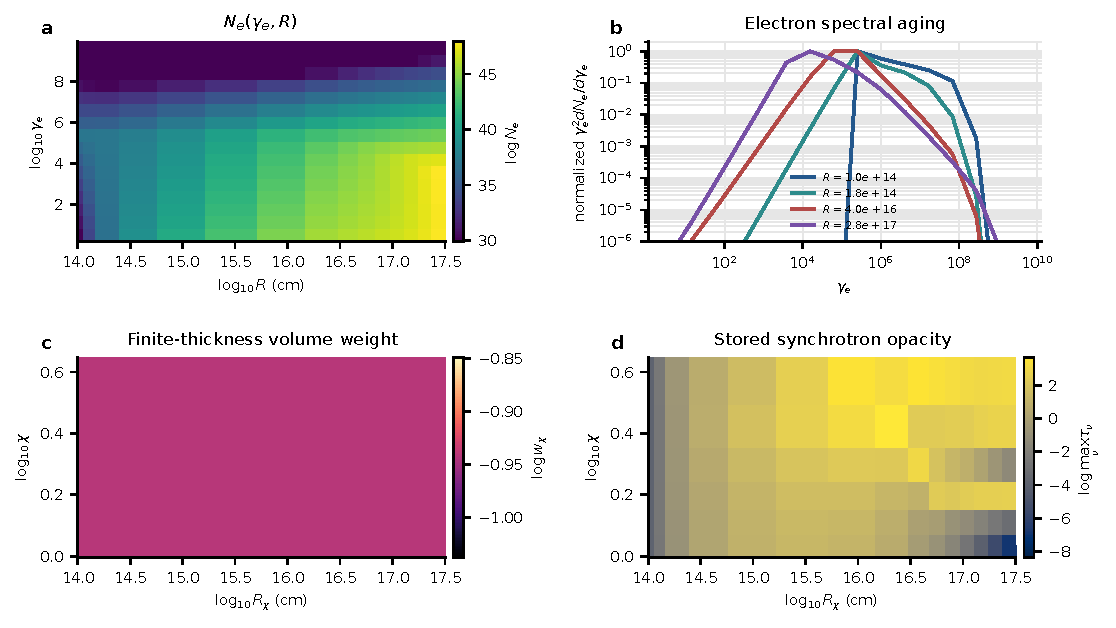
\includegraphics[width=\textwidth]{figures/fig3_transport_projection.pdf}
  \caption{
\gptareaderanchor{gpta-seg-000217}%
观测者投影前的电子和光子状态诊断。
  (a) 一维 \(N_e(\gamma_e,R)\) 状态在径向网格上仍然可见。
  (b) \(\gamma_e^2 dN_e/d\gamma_e\) 的径向切片展示了输运后的电子谱。
  (c) 二维电子运行存储了下游的 \(\chi\) 分辨体积权重。
  (d) 同一运行还存储了由 \(\chi\) 分辨投影使用的同步辐射光学深度场。
  该图记录了所实现的求解器路径中使用的暴露状态；它并非对所有电子输运选项的收敛性证明。}
  \label{fig:electron-transport}
\end{figure*}

热电子具有很窄的求解器边界。它们只在 \texttt{fullhide\_1d} 和 \texttt{fullhide\_1d\_hz} 中实现；其他电子求解器会拒绝热电子输运。自适应电子子步只在选定的一维分离路径中实现，在这些路径中一个完整径向步会与两个半步比较。联合电子--光子耦合使用固定子步，因为次级源和冷却种子会与强子阶段共同迭代。

\subsection{光子场与吸收} \label{sec:photon}

光子场是冷却、SSC、吸收和强子相互作用所使用的辐射靶。电子求解器提供局部同步辐射发射率，并在启用时提供 SSC 发射率。光子模块在任何观测者投影混合半径或角度之前，将这些场存储在共动频率网格上。

\subsubsection{共动靶光子状态}

共动靶光子状态是下一个局部辐射过程读取的光子密度。输入是输运后的电子谱和局部同步辐射发射率。输出是种子频率网格、同步辐射光子场、可选 SSC 光子场、强子靶场，以及同步自吸收和 SSC 吸收使用的种子数组。在分离电子--光子运行中，靶光子密度为
\begin{equation}
\begin{aligned}
n_{\nu'}^{\rm tar}
&=n_{\nu'}^{\rm syn}
+I_{\rm SSC}\,n_{\nu'}^{\rm SSC},\\
I_{\rm SSC}
&=
\begin{cases}
1, & \text{SSC target active},\\
0, & \text{otherwise}.
\end{cases}
\end{aligned}
\end{equation}
这里 \(n_{\nu'}^{\rm syn}\) 和 \(n_{\nu'}^{\rm SSC}\) 是频率 \(\nu'\) 处单位频率的共动光子数密度。开关 \(I_{\rm SSC}\) 决定前向 SSC 光子是否进入靶场。在联合分支中，\(p\gamma\)、Bethe--Heitler 和 \(\gamma\gamma\) 生存因子会在下一次电子求解前作用于 \(n_{\nu'}^{\rm tar}\)。因此，存储的靶场是用于冷却和反馈的局部光子输入，而不是观测者系谱。

\subsubsection{辐射核边界}

辐射核边界把存储的光子状态连接到局部核计算。它不是独立物理模型。公共产物包括 SSC 光度 \(L_{\nu'}^{\rm SSC}\)、局部对吸收因子 \(\mathcal{A}_{\gamma\gamma}\) 和外部 EBL 因子 \(\mathcal{A}_{\rm EBL}\)。散射核、对产生截面、EBL 表格和光子场归一化由下面的物理方程定义。编译核绑定名是 ABI 细节，并记录在附录~\ref{app:photon-kernels} 中。

\subsubsection{辐射插值复用}

辐射插值为每个光子求积在频率节点之间提供相同的局部谱。令 \(X=\ln\nu'\)，\(Y=\ln n_{\nu'}\)。如果两个端点光子密度均为正，则单元在 \((X,Y)\) 中重建为直线，即频率上的局部幂律。如果任一端点非正，则单元在 \(n_{\nu'}\) 中线性重建。该规则返回冷却、SSC 和吸收使用的采样共动光子密度。非递增频率区间位于受支持网格域之外。

\subsubsection{复合 Simpson 辐射求积}

复合 Simpson 求积为均匀 SSC 积分提供数值权重。物理变量为对数形式：种子光子使用 \(x=\ln\nu_s'\)，电子使用 \(x=\ln\gamma\)。在支撑点数为奇数的均匀网格 \(x_i=x_1+(i-1)\Delta x\) 上，该分支使用
\begin{equation}
\begin{aligned}
\int_{x_1}^{x_N} f(x)\,dx
&\simeq
\frac{\Delta x}{3}\sum_{i=1}^{N}w_i^{\rm S} f_i,\\
w_i^{\rm S}
&=
\begin{cases}
1, & i=1 \ \text{or}\ i=N,\\
4, & i \ \text{even},\\
2, & i \ \text{odd and}\ 1<i<N .
\end{cases}
\end{aligned}
\end{equation}
这里 \(f_i=f(x_i)\)，\(w_i^{\rm S}\) 只是求积权重。它不改变电子谱或种子光子密度。该规则返回下面均匀网格 SSC 光度所用的种子频率和电子能量求和；不符合该 Simpson 布局的网格位于此分支之外。

\subsection{均匀网格 SSC 发射率}

\subsubsection{Jones--Klein--Nishina 变量}

前向 SSC 发射来自局部电子对局部同步辐射光子场的散射。均匀网格分支在上文使用的同一对数电子网格和种子频率网格上计算该过程。对于发射共动频率 \(\nu'\) 和种子频率 \(\nu_s'\)，定义
\begin{equation}
\begin{aligned}
\epsilon&=\frac{h\nu'}{m_ec^2},&
\epsilon_s&=\frac{h\nu_s'}{m_ec^2},\\
b&=4\gamma\epsilon_s,&
q&=\frac{\epsilon}{b(\gamma-\epsilon)},\\
\eta&=bq=\frac{\epsilon}{\gamma-\epsilon}.
\end{aligned}
\end{equation}
这里 \(\epsilon\) 是以 \(m_ec^2\) 为单位的发射光子能量，\(\epsilon_s\) 是同一单位下的种子光子能量，\(\gamma\) 是电子洛伦兹因子。变量 \(q\) 和 \(\eta\) 定位 Klein--Nishina 核中的散射事件。对于 \(\nu_s'<\nu'\) 的种子光子，允许的电子能量满足
\begin{equation}
\begin{aligned}
\gamma&>\gamma_{\rm IC},\\
\gamma_{\rm IC}
&\equiv
\frac{1}{2}\left[\epsilon+
\left(\epsilon^2+\frac{\nu'}{\nu_s'}\right)^{1/2}\right].
\end{aligned}
\end{equation}
第一行给出了 \(\gamma\) 的运动学下限。低种子频率积分中使用的 Jones--Klein--Nishina 因子为
\begin{equation}
\begin{aligned}
G(q,\eta)
&=2q\ln q+(1+2q)(1-q)\\
&\quad+\frac{\eta^2(1-q)}{2(1+\eta)} .
\end{aligned}
\label{eq:ssc-kernel}
\end{equation}

\subsubsection{均匀网格 Simpson 积分}

均匀 SSC 光度是两个种子频率范围的和。第一个范围满足 \(\nu_s'<\nu'\)，其中使用完整 Jones--Klein--Nishina 因子。令 \(n_s\equiv n_{\nu_s'}^{\rm tar}\)，该贡献为
\begin{equation}
\begin{aligned}
C_{\rm IC}(\nu')&=\frac{3}{4}ch\sigma_{\rm es}\nu',\\
L_{\nu'}^{{\rm SSC},<}
&=C_{\rm IC}
\int_{\nu_s'<\nu'} d\ln\nu_s'\,n_s
\int d\ln\gamma\,\frac{N_e(\gamma)}{\gamma}
G(q,\eta).
\end{aligned}
\end{equation}
这里 \(\sigma_{\rm es}\) 是电子散射截面，\(n_s\) 是靶光子密度，\(N_e(\gamma)\) 是输运后的电子谱。第二个范围满足 \(\nu_s'\ge\nu'\)。在该范围内，分支使用高能电子尾部矩来计算弹性散射部分，
\begin{equation}
\begin{aligned}
\gamma_{\rm es}(\nu_s')
&=\frac{1}{2}\left(\frac{\nu_s'}{\nu'}\right)^{1/2},\\
\Phi_{\rm es}(\gamma,\nu_s')
&=\frac{\nu'}{\nu_s'}-\frac{1}{4\gamma^2},\\
L_{\nu'}^{{\rm SSC},>}
&=C_{\rm IC}
\int_{\nu_s'\ge\nu'}d\ln\nu_s'\,n_s
\int_{\gamma>\gamma_{\rm es}}d\ln\gamma\,
\frac{N_e(\gamma)}{\gamma}
\Phi_{\rm es}.
\end{aligned}
\end{equation}
两个对数积分都使用上述 Simpson 权重。二者之和给出局部 SSC 光度以及为后续吸收和反馈存储的光子密度：
\begin{equation}
\begin{aligned}
L_{\nu'}^{\rm SSC}
&=L_{\nu'}^{{\rm SSC},<}+L_{\nu'}^{{\rm SSC},>},\\
n_{\nu'}^{\rm SSC}
&=\frac{L_{\nu'}^{\rm SSC}}{4\pi R^2ch\nu'}.
\end{aligned}
\end{equation}
因此，该模块在每个半径处同时返回发射的 SSC 谱和共动 SSC 光子密度。它不改变电子分布；由 SSC 导致的电子冷却由输运步骤处理。

\subsection{非均匀网格 SSC 发射率}

非均匀网格 SSC 分支在单元宽度不等的电子网格上使用同一个散射核。当输运后的电子谱存储在自适应或求解器特定的 \(\ln\gamma\) 单元上时，需要该分支。令 \(x=\ln\gamma\)，\(N_x=dN_e/dx\)。在由 \(x_{i-1/2}\) 和 \(x_{i+1/2}\) 限定的单元 \(i\) 中，该分支重建
\begin{equation}
\begin{aligned}
N_x(x)&\simeq N_{x,i}+s_i(x-x_i),\\
x_i&\equiv \frac{x_{i-1/2}+x_{i+1/2}}{2}.
\end{aligned}
\end{equation}
这里 \(s_i\) 是局部 minmod 限制斜率。该重建提供 SSC 求积内部采样的电子密度；它不修改输运后的电子状态。

非均匀分支改变求积支撑，而不改变康普顿物理。对于 \(\nu_s'<\nu'\)，它在高于运动学下限的每个电子单元上积分同一个 \(G(q,\eta)\) 核，
\begin{equation}
\begin{aligned}
I_i^{<}(\nu',\nu_s')
&=\int_{x_{\rm L}}^{x_{i+1/2}}
N_x(x)\,\frac{G[q(x),\eta(x)]}{\gamma(x)^2}\,dx,\\
x_{\rm L}&=\max[x_{i-1/2},\ln\gamma_{\rm IC}].
\end{aligned}
\end{equation}
种子频率积分和单元积分使用附录~\ref{app:photon-kernels} 中定义的固定 Gauss 规则。对于 \(\nu_s'\ge\nu'\)，该分支使用重建单元的预计算高能矩，
\begin{equation}
\begin{aligned}
M_a(>x_{\rm L})&=\int_{x_{\rm L}}^\infty N_x(x)\gamma(x)^{-a}\,dx,\\
I^{>}(\nu',\nu_s')
&=\frac{\nu'}{\nu_s'}M_2(>x_{\rm L})-\frac{1}{4}M_4(>x_{\rm L}) .
\end{aligned}
\end{equation}
返回的产物仍是 \(L_{\nu'}^{\rm SSC}\) 和 \(n_{\nu'}^{\rm SSC}\)。该分支要求电子单元边界严格递增，并使用同一个种子光子状态 \(n_{\nu'}^{\rm tar}\)；它不定义不同的 SSC 模型 \citep{Jones1968,BlumenthalGould1970}。

\subsection{有限单元光子传递}

\subsubsection{壳层传递因子}

有限单元光子传递把局部光深转换为均匀发射壳层单元的逃逸光度。一个在吸收单元内部产生的光子，平均采样的物质少于一个从外部穿过同一单元的光子。因此，ASGARD 使用方程~(\ref{eq:finite-cell-transfer}) 定义的单元平均因子 \(\psi(\tau)\)，并采用连续极限 \(\psi(0)=1\)。对于同步自吸收，其自变量为
\[
\tau_\nu^{\rm loc}=\alpha_\nu'\Delta r',
\]

\gptareaderanchor{gpta-seg-000218}%
其中 \(\alpha_\nu'\) 是共动吸收系数，\(\Delta r'\) 是共动壳层宽度。对于局域 \(\gamma\gamma\) 吸收，相同的因子用以下方式计算：
\[
\tau_{\gamma\gamma}^{\rm loc}(\nu')
=\Delta r'\int \sigma_{\gamma\gamma}(\nu',\tilde\nu')
n_{\tilde\nu'}^{\rm tar}\,d\tilde\nu' .
\]

\gptareaderanchor{gpta-seg-000219}%
因此，传递步骤仅改变逃逸光子光度与存储光子密度。它不改变光子产生核或输运电子谱。

\subsection{\texorpdfstring{\(\gamma\gamma\)}{gamma-gamma} 壳层吸收}

\subsubsection{软光子单元测度}


\gptareaderanchor{gpta-seg-000220}%
配对吸收通过将高能光子与本地目标光子场碰撞来移除该光子。该内核首先将种子频率网格转换为无量纲的光子能量和细胞度量。对于一个协动频率为\(\nu_1'\)的光子和一个目标频率细胞\((\nu_j',\nu_{j+1}')\)，定义
\begin{equation}
\begin{aligned}
\epsilon_1&=\frac{h\nu_1'}{m_ec^2},\\
\nu_{2,j}'&=(\nu_j'\nu_{j+1}')^{1/2},\\
\epsilon_{2,j}&=\frac{h\nu_{2,j}'}{m_ec^2},\\
\Delta\nu_j'&=\nu_{2,j}'\Delta\ln\nu' .
\end{aligned}
\end{equation}

\gptareaderanchor{gpta-seg-000221}%
这里 \(\epsilon_1\) 和 \(\epsilon_{2,j}\) 是以 \(m_ec^2\) 为单位的光子能量，而 \(\Delta\nu_j'\) 是由对数目标单元表示的频率宽度。该单元中采样的目标密度为 \(n_{\nu_{2,j}'}^{\rm tar}\)。

\subsubsection{各向同性角矩}


\gptareaderanchor{gpta-seg-000222}%
对于局部共动各向同性靶场，定义
\(x_j\equiv\epsilon_1\epsilon_{2,j}\) 和
\(z\equiv(1-\mu)/2\)。包含光子相对速度权重的角平均为
\begin{equation}
\begin{aligned}
K(x)&=\frac{1}{2}\int_{-1}^{1}(1-\mu)
\sigma_{\gamma\gamma}\!\left[x\frac{1-\mu}{2}\right]d\mu\\
&=2\int_{1/x}^{1}z\,\sigma_{\gamma\gamma}(xz)\,dz,
\qquad x>1,
\end{aligned}
\end{equation}
且当 \(x\le1\) 时 \(K(x)=0\)。因此，物理对产生阈值直接确定积分支撑区间，
无需对 \(s=xz\) 引入上截断。

\gptareaderanchor{gpta-seg-000223}%
Breit--Wheeler 截面写为
\begin{equation}
\begin{aligned}
u_s&=s^{-1},\qquad \beta_s=(1-u_s)^{1/2},\\
L_s&=\ln\frac{1+\beta_s}{1-\beta_s}
=\ln s+2\ln(1+\beta_s),\\
\sigma_{\gamma\gamma}(s)&=
\begin{cases}
\dfrac{3\sigma_{\rm es}}{16}u_s
\left[(3-\beta_s^4)L_s-2\beta_s(2-\beta_s^2)\right], & s>1,\\
0, & s\le1 .
\end{cases}
\end{aligned}
\end{equation}

\gptareaderanchor{gpta-seg-000224}%
在阈值附近，实现采用 \(\beta_s^2=(s-1)u_s\)，并以等价的
\(\operatorname{atanh}\) 恒等式计算对数。在大 \(s\) 区域，\(u_s\) 与 \(L_s\)
避免了相减两个近乎相等的浮点数。对于每个 \(x>1\)，变量代换
\(s=1+(x-1)t^2\) 给出
\begin{equation}
K(x)=\frac{4(x-1)}{x^2}\int_0^1
t\,s(t)\,\sigma_{\gamma\gamma}[s(t)]\,dt .
\end{equation}
实现对 \(0<t<1\) 上的这一光滑积分采用 16 点 Gauss--Legendre 求积。

\subsubsection{壳层光深组装}


\gptareaderanchor{gpta-seg-000225}%
角矩与壳层半径无关，因此可在组装靶场时复用。对于半径 \(R_i\)、洛伦兹因子
\(\Gamma_i\) 的壳层，定义
\begin{equation}
\begin{aligned}
\Delta'_{\gamma\gamma,i}&=\frac{R_i}{12\Gamma_i},\\
n_j&=n_{\nu_{2,j}'}^{\rm tar}(R_i),\\
\tau_{\gamma\gamma}(\nu_1',R_i)
&=\Delta'_{\gamma\gamma,i}
\sum_j K(x_j)n_j\Delta\nu_j'
+\tau_{\rm ex}(\nu_1',R_i).
\end{aligned}
\end{equation}

\gptareaderanchor{gpta-seg-000226}%
这里不再乘额外的 \(1/2\)，因为 \(K\) 已包含各向同性角归一化。
该路径长度仅是当前 \(k=0\) 均匀壳层近似：
\(N_{\rm sw}=4\pi nR^3/3=(4\pi R^2\Delta')(4\Gamma n)\) 给出
\(\Delta'=R/(12\Gamma)\)。该均匀壳层估计采用 \(n_2'=4\Gamma n\)；它既不是
任意 \(\Gamma\) 下精确的压缩关系，也不是一般的 Blandford--McKee 壳层宽度。
跨相对论区的压缩与路径长度、\(k=2\) 风介质、表格密度跃变、prompt 内激波和级联区
仍是当前实现中已登记的适用边界。\(\tau_{\rm ex}\) 添加其他局部模块给出的光学深度。
返回的有限单元存活因子为
\begin{equation}
\begin{aligned}
\mathcal{A}_{\gamma\gamma}(\nu_1',R_i)
&=\psi[\tau_{\gamma\gamma}(\nu_1',R_i)] .
\end{aligned}
\end{equation}

\gptareaderanchor{gpta-seg-000227}%
该因子衰减了在整个吸收细胞内发射的光子。它不是前景屏因子\(e^{-\tau}\)。输出是光子集合所使用的局部\(\gamma\gamma\)衰减\citep{GouldSchreder1967,Svensson1987}。

\subsection{正面碰撞路径不透明度辅助器}


\gptareaderanchor{gpta-seg-000228}%
正面碰撞辅助器为光子历史传输提供路径光学深度。它不是上述的外壳发射衰减。它仅保留正面碰撞不变量 \(s_j^{\rm ho}\equiv\epsilon_1\epsilon_{2,j}\)。对于共动路径长度 \(\Delta x'\)，它计算
\begin{equation}
\begin{aligned}
\tau_{\gamma\gamma}^{\rm ho}(\nu_1')=
\Delta x'
\sum_j \sigma_{\gamma\gamma}(s_j^{\rm ho})
n_{\nu_{2,j}'}^{\rm tar}\Delta\nu_j' .
\end{aligned}
\end{equation}

\gptareaderanchor{gpta-seg-000229}%
该辅助函数返回射线线段的路径不透明度。它不替代用于壳层发射的角度平均有限单元存活率计算。

\subsection{外部 EBL 衰减}

\subsubsection{表格边界}


\gptareaderanchor{gpta-seg-000230}%
外部EBL衰减是指背景光子在抵达观测者的宇宙学路径上的吸收。该过程作用于光子离开局部激波壳层之后，因此不属于壳层光子密度、电子冷却或\(\gamma\gamma\)反馈的组成部分。默认采用Domínguez等人的表格\citep{Dominguez2011EBL}提供的光学深度网格，其行对应光子能量\(E_i\)，列对应源的红移\(z_j\)。代码使用相应的观测频率。
\begin{equation}
\begin{aligned}
\nu_i=\frac{E_i}{h}, \qquad
\tau_{\rm EBL}(\nu_i,0)=0 .
\end{aligned}
\end{equation}

\gptareaderanchor{gpta-seg-000231}%
第二个关系是零距离边界。它表明，在\(z=0\)处的源在此表中没有宇宙学EBL路径。

\subsubsection{红移与频率插值}


\gptareaderanchor{gpta-seg-000232}%
EBL表格只给出了离散的红移和离散的光子能量。对于源红移位于 \(z_j\) 和 \(z_{j+1}\) 之间的情况，代码首先形成红移权重。
\begin{equation}
\begin{aligned}
\lambda_z&=\frac{z-z_j}{z_{j+1}-z_j},\\
\tau_i(z)&=(1-\lambda_z)\tau_{ij}
+\lambda_z\tau_{i,j+1}.
\end{aligned}
\end{equation}

\gptareaderanchor{gpta-seg-000233}%
这里 \(\tau_{ij}\) 是在 \((\nu_i,z_j)\) 处的列表光深。然后该代码在观测频率上进行插值。对于 \(\nu_i\le\nu_{\rm obs}\le\nu_{i+1}\)，
\begin{equation}
\begin{aligned}
\lambda_\nu&=\frac{\nu_{\rm obs}-\nu_i}{\nu_{i+1}-\nu_i},\\
\tau_{\rm EBL}(\nu_{\rm obs},z)=
(1-\lambda_\nu)\tau_i(z)+\lambda_\nu\tau_{i+1}(z).
\end{aligned}
\end{equation}

\gptareaderanchor{gpta-seg-000234}%
低于列表中最小的伽马射线能量时，返回的光学深度为零。对于\(z<0\)的情况，或当\(z\)大于列表中的最大红移，或\(\nu_{\rm obs}\)大于列表中的最大频率时，所选的EBL模型未定义衰减因子。

\subsubsection{外部衰减因子}


\gptareaderanchor{gpta-seg-000235}%
EBL输出是观测者侧通量的一个单一乘法因子。它是
\begin{equation}
\begin{aligned}
\mathcal{A}_{\rm EBL}(\nu_{\rm obs},z)
=\exp[-\tau_{\rm EBL}(\nu_{\rm obs},z)].
\end{aligned}
\end{equation}

\gptareaderanchor{gpta-seg-000236}%
这个因子是一种外部观测者侧产物。它可以在局部传输后乘以投影通量，但不会改变任何局部粒子或光子的状态。

\subsection{观测者侧光子分量组装}

\subsubsection{分量排序}


\gptareaderanchor{gpta-seg-000237}%
观测端光子组装是在局部辐射模块完成后进行的组件核算。前向同步辐射光度在标准前向激波运行中始终存在，而前向SSC仅在SSC求解器激活时存在。反向激波同步辐射、反向SSC、反向强子发射以及跨区逆康普顿发射仅在反向激波状态提供这些光度时进入。前向强子伽马射线、贝特--海特勒、强子逆康普顿以及电子对产生组件仅在一维强子分支提供它们时进入。因此，活跃集为
\begin{equation}
\begin{aligned}
{\cal C}_{\rm act}\subset
\{&{\rm FS\,syn},{\rm FS\,SSC},{\rm FS\,had},{\rm FS\,BH},
{\rm FS\,HIC},{\rm FS\,pair},\\
&{\rm RS\,syn},{\rm RS\,had},{\rm RS\,SSC},{\rm cross\,IC}\}.
\end{aligned}
\end{equation}

\gptareaderanchor{gpta-seg-000238}%
在观察者组装过程中，缺失的组件不会被重建。

\subsubsection{距离与衰减前因子}


\gptareaderanchor{gpta-seg-000239}%
距离和衰减前置因子将每个活跃的本地光度转换为径向通量网格，然后进行等到达时间投影。对于通道 \(a\in{\cal C}_{\rm act}\)，令 \(\widetilde L_{\nu'}^a(R)\) 表示该通道自身壳层传输后的本地光谱光度。组装步骤使用
\begin{equation}
\begin{aligned}
\mathcal{P}_{\rm loc}(\nu,R)&=
\frac{1+z}{4\pi d_L^2}\,
\mathcal{A}_{\rm loc}(\nu,R),\\
\Delta F_\nu^a(R)&=
\mathcal{P}_{\rm loc}(\nu,R)\,\widetilde L_{\nu'}^a(R),\\
F_\nu^{\rm rad}(R)&=
\sum_{a\in{\cal C}_{\rm act}}\Delta F_\nu^a(R).
\end{aligned}
\end{equation}

\gptareaderanchor{gpta-seg-000240}%
这里\(d_L\)是光度距离，\(\mathcal{A}_{\rm loc}\)是双光子吸收核返回的局部光子生存因子，包括了活跃的额外光学深度，如Bethe–Heitler光子损失和级联对的不透明度。EBL表格因子相对于这个局部前置因子是外部的。然后投影模块将每个\(\Delta F_\nu^a(R)\)和求和后的\(F_\nu^{\rm rad}(R)\)映射到观测者时间。

\section{反向激波与密度跃变次级激波} \label{sec:reverse-shock}

\subsection{主抛射物状态与激活}

\subsubsection{物理作用}


\gptareaderanchor{gpta-seg-000241}%
主反向激波加热原始抛射壳层。它与加热外部介质的正向激波不同。因此，这一分支需要有限的壳层宽度、区域-4的上游密度，以及判定磁化上游流何时能形成激波的规则。其输出结果为区域-3的质量、热能、体积、磁场和电子注入尺度。

\subsubsection{激活边界}


\gptareaderanchor{gpta-seg-000242}%
反向激波分支仅在输入模型提供引擎持续时间时才处于活动状态。该持续时间决定了初始壳层宽度，因此若无此参数，程序将无法获取反向激波上游区域4的密度。我们将初始抛射体的洛伦兹因子记为\(\Gamma_0\)；运行时字段\(\eta_0\)存储相同的数值。

\subsubsection{抛射物壳层状态}


\gptareaderanchor{gpta-seg-000243}%
抛射物壳层状态给出了反向激波所观测到的重子密度和惯性。对于引擎持续时间 \(\Delta t_{\rm eng}\)，\asgard 使用
\begin{equation}
\begin{aligned}
\Delta_0&\equiv c\Delta t_{\rm eng},\\
M_{\rm ej}&\equiv \frac{E_{\rm iso}}{(1+\sigma)\Gamma_0c^2},\\
\Delta(R)&\equiv \max\left(\Delta_0,\frac{R}{\Gamma_0^2}\right),\\
n_4(R)&\equiv \frac{M_{\rm ej}}
{4\pi m_pR^2\Gamma_0\Delta(R)} .
\end{aligned}
\end{equation}

\gptareaderanchor{gpta-seg-000244}%
这里 \(\Delta_0\) 是初始壳层宽度，\(\Delta(R)\) 包含径向扩散，\(M_{\rm ej}\) 是重子抛射物质量，\(n_4\) 是区域4中的上游重子密度。总抛射物能量为 \(E_{\rm iso}\)。当 \(\sigma>0\) 时，只有 \((1+\sigma)^{-1}\) 的部分由重子静止质量承载。未受激波的壳层仍包含物质与有序场惯性，因此 \asgard\ 使用 \(n_4\) 进行激波加热和电子注入，但在未处理的磁化抛射物进入惯性预算时，使用 \(\tilde n_4\equiv(1+\sigma)n_4\)。

\subsubsection{激波前沿相对洛伦兹因子}


\gptareaderanchor{gpta-seg-000245}%
反向激波电子源由激波前沿的局部相对洛伦兹因子决定。若 \(\Gamma_2\) 为受激壳层洛伦兹因子，\(\Gamma_0\) 为未受激喷射物洛伦兹因子，则
\begin{equation}
\begin{aligned}
u_2&=(\Gamma_2^2-1)^{1/2},\\
u_0&=(\Gamma_0^2-1)^{1/2},\\
\gamma_{34}&=\Gamma_2\Gamma_0-u_2u_0.
\end{aligned}
\end{equation}

\gptareaderanchor{gpta-seg-000246}%
这里 \(u_2\) 和 \(u_0\) 分别是受激壳层和未受激喷射物的四速。输出 \(\gamma_{34}(R)\) 设定了区域3电子的反向激波注入能量标度。

\subsubsection{磁化激活判据}


\gptareaderanchor{gpta-seg-000247}%
磁化喷出物只有在两个局部条件成立时才会形成反向激波。区域2的压力必须足够大以抵抗上游有序场，同时上游流在反向激波参考系中必须是超快磁声波的。压力条件写作
\begin{equation}
\begin{aligned}
P_2&\equiv
\frac{(4\Gamma_2+3)(\Gamma_2-1)n_1m_pc^2}{3},\\
\sigma_{\rm cr}&\equiv \frac{2P_2}{n_4m_pc^2},
\end{aligned}
\end{equation}

\gptareaderanchor{gpta-seg-000248}%
其中 \(P_2\) 是区域2的压力估计值，\(n_1\) 是外部上游密度。主动条件是
\begin{equation}
\sigma_{\rm cr}\ge\sigma,\qquad u_{4s}^2>\sigma ,
\end{equation}

\gptareaderanchor{gpta-seg-000249}%
其中\(u_{4s}\)是反向激波参考系中区域4的上游四速。
第一个不等式是压力判据，第二个是快磁声波判据。对于\(\sigma\le0\)，这些磁化激活检查不会延迟流体动力学反向激波。

\subsubsection{等待态惯性}


\gptareaderanchor{gpta-seg-000250}%
等待状态让磁化喷射物在添加反向激波热量之前先增加惯性。在激活检查通过之前，\(dM_3/dR=0\)，不添加区域3的热能，不注入反向激波电子，且有序的区域3磁场为零。减速的激波壳层仍感受到未受激喷射物中因果连接的部分。
\begin{equation}
\begin{aligned}
M_{\rm w}&\equiv
M_{\rm ej}(1+\sigma)\frac{\Gamma_0}{\Gamma_0-1}f_{\rm f},\\
\beta_{\rm f}&\equiv \left(\frac{\sigma}{1+\sigma}\right)^{1/2},\\
f_{\rm f}&\equiv \min\left[
1,\,
\frac{R\beta_{\rm f}}
{\Gamma_0^2(1-\beta_4\beta_{\rm f})\beta_4\Delta(R)}
\right].
\end{aligned}
\end{equation}

\gptareaderanchor{gpta-seg-000251}%
这里 \(M_{\rm w}\) 是等待喷出物的惯性，\(\beta_{\rm f}\) 是以光速 \(c\) 为单位的快磁声速，\(f_{\rm f}\) 是连接的壳层比例，\(\beta_4\) 是区域4速度。等待阶段的洛伦兹因子遵循
\begin{equation}
\frac{d\Gamma_2}{dR}
=-\frac{u_2^2\,dM_2/dR}
{M_{\rm w}+[\epsilon_2+2(1-\epsilon_2)\Gamma_2]M_2}.
\end{equation}

\gptareaderanchor{gpta-seg-000252}%
该方程使用了正向扫过的质量 \(M_2\) 和辐射效率
\(\epsilon_2\)，但不包含反向激波质量或热源。当
两个激活条件在一个径向步长内首次成立时，\asgard\ 定位该
事件并在该处启动主动反向激波状态。反向激波
框架遵循早期余辉薄壳/反向激波处理方法以及
Zhang--Kobayashi 型计算中使用的磁化抛射物记号，同时
仅将 \vegas\ 用作跳变条件比较后端
\citep{SariPiran1999,Kobayashi2000,ZhangKobayashi2005,PeerWijers2006,Giannios2008,Wang2025VegasAfterglow}。

\subsection{有限强度 MHD 跃变求解器}

\subsubsection{冷上游变量}


\gptareaderanchor{gpta-seg-000253}%
MHD跳跃求解器给出了磁化反向激波产生的压缩和热量。上游喷出物是冷的，并携带横向有序磁场。局部相对洛伦兹因子是
\begin{equation}
\begin{aligned}
g&\equiv\gamma_{34},\qquad
\hat{\gamma}\equiv \frac{4}{3}+\frac{1}{3g}.
\end{aligned}
\end{equation}

\gptareaderanchor{gpta-seg-000254}%
这里，\(g\) 表示反向激波的强度，\(\hat{\gamma}\) 是跳跃关系中使用的局部绝热指数代理。当 \(\sigma>\sigma_{\rm cut}\) 时，下游激波系中的四速度由 \(y=u_d^2\) 求出：
\begin{equation}
\begin{aligned}
a_3y^3+a_2y^2+a_1y+a_0&=0,\\
u_d&=y^{1/2}.
\end{aligned}
\end{equation}

\gptareaderanchor{gpta-seg-000255}%
系数 \(a_i(g,\hat{\gamma},\sigma)\) 是附录~\ref{app:reverse-shock-technical}中给出的固定有限强度MHD跳跃系数。量 \(\sigma_{\rm cut}\) 仅用于选择实现所使用的代数分支；它并非物理磁化边界。

\subsubsection{三次方程根选择}


\gptareaderanchor{gpta-seg-000256}%
三次根选择选取有限的正向下游四速度。求解器将多项式化为缺项三次方程并取根。
\begin{equation}
\begin{aligned}
y&=2a_c\cos\left(\psi_c-\frac{2\pi}{3}\right)-\frac{b_c}{3},\\
u_d&=y^{1/2}.
\end{aligned}
\end{equation}

\gptareaderanchor{gpta-seg-000257}%
符号 \(b_c\)、\(a_c\) 和 \(\psi_c\) 是附录~\ref{app:reverse-shock-technical} 中定义的降阶三次变量。壳层动力学中未使用其他代数根。

\subsubsection{压缩比}


\gptareaderanchor{gpta-seg-000258}%
压缩比由上游和下游激波框架的四速度得出。一旦 \(u_d\) 已知，上游四速度和压缩比
\begin{equation}
\begin{aligned}
u_u&=\left[(1+u_d^2)(g^2-1)\right]^{1/2}+u_dg,\\
r_\sigma&=\frac{u_u}{u_d}.
\end{aligned}
\end{equation}

\gptareaderanchor{gpta-seg-000259}%
这里\(u_u\)是激波参考系中的上游四速度。输出量\(r_\sigma\)压缩有序的上游磁场，并设定通过活跃的主反向激波的质量通量。

\subsubsection{\texorpdfstring{低 \(\sigma\)}{Low-sigma} 流体动力学分支}


\gptareaderanchor{gpta-seg-000260}%
低\(\sigma\)分支采用有限强度流体动力学极限。对于\(\sigma\le\sigma_{\rm cut}\)，\asgard 使用
\begin{equation}
\begin{aligned}
y_{\rm h}&=
\frac{(g-1)(\hat{\gamma}-1)^2}
{-\hat{\gamma}(\hat{\gamma}-2)(g-1)+2},\\
u_d&=y_{\rm h}^{1/2},\\
r_0&=4g .
\end{aligned}
\end{equation}

\gptareaderanchor{gpta-seg-000261}%
热辅助函数对于完全无磁化的喷射物返回\(g-1\)。当\(0<\sigma\le\sigma_{\rm cut}\)时，它计算有限\(\sigma\)的焓，并随着\(\sigma\)减小而趋近于\(g-1\)。主动动力学不使用超相对论\(4g+3\)压缩近似。这个MHD激波仅由主喷射物反向激波使用。下方的密度跳跃次级分支仍然是流体力学诊断，不携带有序场压缩或磁焓反馈。

\subsection{共动区域3磁场与热状态}

\subsubsection{上游有序场}


\gptareaderanchor{gpta-seg-000262}%
上游有序场是未受激的喷射物在穿过反向激波之前携带的磁场。本小节中的所有磁场均为共动场。对于区域4的重子密度 \(n_4\)，
\begin{equation}
\begin{aligned}
\rho_4&\equiv m_pn_4,\\
B'_4&\equiv (4\pi\sigma\rho_4c^2)^{1/2}.
\end{aligned}
\end{equation}

\gptareaderanchor{gpta-seg-000263}%
这里 \(\rho_4\) 是共动重子质量密度，而 \(B'_4\) 是压缩前有序上游场。若 \(\sigma=0\)，则该有序分量为零。

\subsubsection{区域3湍动场与有序场}


\gptareaderanchor{gpta-seg-000264}%
区域-3的磁场由冲击加热产生的湍流部分和从喷射物场压缩的有序部分组成。在活跃的前穿越过程中，\asgard\ 储存
\begin{equation}
\begin{aligned}
B_{\rm t}^{\prime 2}&\equiv 8\pi\epsilon_{B,r}\frac{U_3}{V_3},\\
B'_{\rm o}&=r_\sigma B'_4 \qquad \hbox{before crossing},\\
B'_3&=\left(B_{\rm t}^{\prime 2}+B_{\rm o}^{\prime 2}\right)^{1/2},
\end{aligned}
\end{equation}

\gptareaderanchor{gpta-seg-000265}%
其中\(U_3\)和\(V_3\)分别是区域3的内能和共动体积。总场\(B'_3\)对应于反向激波辐射状态，并用于局部区域3的同步辐射冷却尺度。只有有序部分\(B'_{\rm o}\)对整体动力学中的磁焓项有贡献。在等待状态下，没有反向激波热量加入，且\(B'_3=0\)。

\subsubsection{穿越后有序场平流}


\gptareaderanchor{gpta-seg-000266}%
跨后有序场在反向激波穿过抛射壳层后得以携带。存储的穿越值随区域3的体积和半径演化，如
\begin{equation}
B'_{\rm o}(R)=B'_{{\rm o},\times}
\frac{V_{3,\times}}{V_3(R)}
\frac{R}{R_\times}.
\end{equation}

\gptareaderanchor{gpta-seg-000267}%
这里 \(R_\times\)、\(V_{3,\times}\) 和 \(B'_{{\rm o},\times}\) 分别是壳层穿越处的半径、体积和有序场。穿越场是一种事件注册状态。它不是在光变曲线计算之后进行拟合的。

\subsubsection{磁焓惯性}


\gptareaderanchor{gpta-seg-000268}%
磁焓惯性是有序场中反作用于壳层动力学的部分。对于有序分量，
\begin{equation}
\begin{aligned}
p_B&\equiv \frac{B_{\rm o}^{\prime 2}}{8\pi},\\
E_B&\equiv p_BV_3 .
\end{aligned}
\end{equation}

\gptareaderanchor{gpta-seg-000269}%
添加到\(\Gamma_2\)方程中的惯性是
\begin{equation}
M_B=\frac{E_B+p_BV_3}{c^2}+\frac{p_BV_3}{\Gamma_2^2c^2}.
\end{equation}

\gptareaderanchor{gpta-seg-000270}%
第一项是磁焓贡献。第二项是由壳层方程保留的有限\(\Gamma_2\)压力贡献。

\subsubsection{跃变给出的热状态}


\gptareaderanchor{gpta-seg-000271}%
来自跳变的热态提供了可用于区域3电子的热能。\asgard\ 使用无量纲热。
\begin{equation}
\begin{aligned}
\zeta_3&\equiv\frac{U_3}{M_3c^2},\\
\gamma_u&\equiv(1+u_u^2)^{1/2},\\
\gamma_d&\equiv(1+u_d^2)^{1/2}.
\end{aligned}
\end{equation}

\gptareaderanchor{gpta-seg-000272}%
这里 \(M_3\) 是激波喷射物质量，而 \(u_u\) 和 \(u_d\) 分别是从跳跃解得到的上游和下游冲击波框架的四速度。在主动预交叉期间，
\begin{equation}
\begin{aligned}
\zeta_3&=\frac{h_d-1}{\hat{\gamma}},\\
h_d&\equiv (1+\sigma)\frac{\gamma_u}{\gamma_d}-r_\sigma\sigma .
\end{aligned}
\end{equation}

\gptareaderanchor{gpta-seg-000273}%
因此，在磁化活跃时，\(\zeta_3\)（而非无磁化估计 \(\gamma_{34}-1\)）决定了反向激波加热。洛伦兹方程中的热响应因子是
\begin{equation}
\mathcal R_3=
\begin{cases}
1, & \sigma=0,\\
\zeta_3/(\gamma_{34}-1), & \sigma>0,
\end{cases}
\end{equation}

\gptareaderanchor{gpta-seg-000274}%
因此，MHD激波改变了主反向激波动力学的两个部分：显式磁惯性 \(M_B\)，以及通过 \(\mathcal R_3\) 产生的受激喷射物质热量与整体运动之间的耦合。在壳层穿越之后，代码使用演化的比值 \(U_3/(M_3c^2)\)，并将这个穿越前的响应项设为零。

\subsection{主反向激波 ODE}

\subsubsection{状态向量与归一化}


\gptareaderanchor{gpta-seg-000275}%
主要的反向激波ODE演化了一个由前向激波介质和反向激波喷射物共享的接触不连续面。状态向量存储了整体运动和区域3的热力学状态。
\begin{equation}
\begin{aligned}
Y_{\rm R}&\equiv
\left(\Gamma_2,R,M_2,\frac{M_3}{M_{\rm ej}},
\frac{U_3}{M_{\rm ej}c^2},\frac{V_3}{V_0},\ldots\right),
\end{aligned}
\end{equation}

\gptareaderanchor{gpta-seg-000276}%
其中省略号表示密度跳跃次级激波的记录。前向扫过的质量和体积归一化是
\begin{equation}
\begin{aligned}
\frac{dM_2}{dR}&=4\pi R^2m_pn_1,\\
V_0&\equiv \frac{M_{\rm ej}}{n_{3,0}m_p}.
\end{aligned}
\end{equation}

\gptareaderanchor{gpta-seg-000277}%
这里 \(n_1\) 是外部密度，而 \(V_0\) 仅是积分器所使用的共动体积归一化。因此，前六个分量映射到物理导数，如下所示：
\begin{equation}
\begin{aligned}
\frac{dY_1}{dt}&=\frac{d\Gamma_2}{dt},&
\frac{dY_2}{dt}&=\frac{dR}{dt},&
\frac{dY_3}{dt}&=\frac{dM_2}{dt},\\
\frac{dY_4}{dt}&=\frac{1}{M_{\rm ej}}\frac{dM_3}{dt},&
\frac{dY_5}{dt}&=\frac{1}{M_{\rm ej}c^2}\frac{dU_3}{dt},&
\frac{dY_6}{dt}&=\frac{1}{V_0}\frac{dV_3}{dt}.
\end{aligned}
\end{equation}

\gptareaderanchor{gpta-seg-000278}%
撤销此归一化后，导出的态是物理的。

\subsubsection{穿越前质量通量}


\gptareaderanchor{gpta-seg-000279}%
跨越前的质量通量表明了未受激抛射物进入区域3的速度。在壳层跨越之前，反向激波从区域4的密度\(n_4\)中扫过重子：
\begin{equation}
\begin{aligned}
\frac{dM_3}{dt}&=
4\pi R^2m_p\,\Gamma_0 n_4\,\Delta\beta_{\rm rs}
\frac{dR}{dt},\\
\frac{dR}{dt}&=\frac{\beta_2c}{1-\beta_2}.
\end{aligned}
\end{equation}

\gptareaderanchor{gpta-seg-000280}%
这里 \(\Delta\beta_{\rm rs}\) 是反向激波波前相对于未受激喷出物在实验室坐标系径向坐标中的速度。该源在等待状态和壳层穿越后为零。

\subsubsection{反向激波速度}


\gptareaderanchor{gpta-seg-000281}%
逆激波前沿的速度由上游激波参考系中的四速度得到。实验室参考系中的逆激波速度为
\begin{equation}
\beta_{\rm rs}=\beta_4-\Delta\beta_{\rm rs},
\end{equation}
with
\begin{equation}
\Delta\beta_{\rm rs}
=\frac{u_u}
{\Gamma_0(\Gamma_0\gamma_u-u_0u_u)}.
\end{equation}

\gptareaderanchor{gpta-seg-000282}%
此处，\(u_0 = (\Gamma_0^2 - 1)^{1/2}\)，而 \(u_u\) 和 \(\gamma_u\) 由MHD跳跃解提供。该定义将质量通量与激波前沿的跳跃状态直接关联。

\subsubsection{活动穿越前洛伦兹方程}


\gptareaderanchor{gpta-seg-000283}%
主动跨越前洛伦兹方程平衡了前向扫掠质量、反向激波载荷、热惯性、磁惯性和主动二次激波惯性。在这一分支中，
\begin{equation}
\begin{aligned}
\mathcal A_{\rm pre}
&\equiv(\Gamma_2^2-1)n_1+\mathcal B_{\rm pre},\\
\mathcal B_{\rm pre}
&\equiv(\Gamma_2\gamma_{34}-\Gamma_0)\Delta\beta_{\rm rs}
\Gamma_0\tilde n_4,\\
\frac{d\Gamma_2}{dR}
=-\frac{4\pi R^2m_p\mathcal A_{\rm pre}}{\mathcal I_{\rm pre}}.
\end{aligned}
\end{equation}

\gptareaderanchor{gpta-seg-000284}%
这里 \(\tilde n_4=(1+\sigma)n_4\) 是未处理磁化喷出物的惯性密度。\(\mathcal A_{\rm pre}\) 中的第一项是正向激波减速，而 \(\mathcal B_{\rm pre}\) 是反向激波加载。惯性分母是
\begin{equation}
\begin{split}
\mathcal I_{\rm pre}={}&
[\epsilon_2+2(1-\epsilon_2)\Gamma_2]M_2
+M_3+M_B+M_s \\
& +(1-\epsilon_3)\zeta_3M_3
+(1-\epsilon_3)\Gamma_2\mathcal R_3M_3\mathcal G_{34}.
\end{split}
\end{equation}

\gptareaderanchor{gpta-seg-000285}%
这里\(M_s\)是活跃的流体力学次级反向激波分支的有效惯性。当没有密度跳跃分支活跃时，它为零。最后一个因子是\(\gamma_{34}\)关于\(\Gamma_2\)的导数，
\begin{equation}
\mathcal G_{34}=
\Gamma_0(1-\beta_4\beta_2)
-\frac{\Gamma_0\beta_4}{\Gamma_2^2\beta_2}.
\end{equation}

\gptareaderanchor{gpta-seg-000286}%
该方程仅在主动前穿越期间使用。等待和后穿越状态则使用上文和下文所述的独立方程。

\subsubsection{反向辐射份额}


\gptareaderanchor{gpta-seg-000287}%
反向辐射分数控制了冲击抛射物热量中保留在惯性项中的部分。\asgard\ 使用与前向动力学相同的冷却诊断方法来计算它。
\begin{equation}
\begin{aligned}
\gamma_{c,3}&=\frac{6\pi m_ec}
{\sigma_{\rm es} B_3^{\prime 2}\Gamma_2t},\\
\gamma_{m,3}&=1+
\frac{\epsilon_{e,r}}{f_{e,r}}
\frac{p_r-2}{p_r-1}
\frac{m_p}{m_e}\zeta_3,
\end{aligned}
\end{equation}
\begin{equation}
\epsilon_3=\epsilon_{e,r}\min\left[
1,\left(\frac{\gamma_{m,3}}{\gamma_{c,3}}\right)^{p_r-2}
\right].
\end{equation}

\gptareaderanchor{gpta-seg-000288}%
这里 \(t\) 是动力学使用的源帧时间，\(B'_3\) 是跳跃与加热状态返回的总区域3场，而 \(p_r\)、\(f_{e,r}\) 和 \(\epsilon_{e,r}\) 是反向激波电子参数。

\subsubsection{热量与体积更新}


\gptareaderanchor{gpta-seg-000289}%
热更新在区域3中增加冲击热量并减去绝热功：
\begin{equation}
\frac{dU_3}{dt}=\zeta_3c^2\frac{dM_3}{dt}
-(\hat{\gamma}_{3}-1)\frac{U_3}{V_3}q_{V,3},
\end{equation}
\begin{equation}
\begin{aligned}
\gamma_{{\rm th},3}&=1+\zeta_3,\\
\hat{\gamma}_{3}&=
\frac{4\gamma_{{\rm th},3}+1}{3\gamma_{{\rm th},3}},
\end{aligned}
\end{equation}

\gptareaderanchor{gpta-seg-000290}%
其中\(\gamma_{{\rm th},3}\)是热洛伦兹因子代理，\(\hat{\gamma}_3\)是区域3的绝热指数。体积更新为
\begin{equation}
\begin{aligned}
\frac{dV_3}{dt}&=\frac{1}{r_\sigma n_4m_p}\frac{dM_3}{dt}
+q_{V,3},\\
q_{V,3}&\equiv V_3\left(\frac{3}{R}\frac{dR}{dt}
-\frac{1}{\Gamma_2}\frac{d\Gamma_2}{dt}\right).
\end{aligned}
\end{equation}

\gptareaderanchor{gpta-seg-000291}%
第一项增加了新冲击的体积，而\(q_{V,3}\)给出了已冲击区域的整体膨胀。在等待状态下，两项均为零。穿过之后，只剩下膨胀项。

\subsubsection{穿越后整体更新}


\gptareaderanchor{gpta-seg-000292}%
跨过后的整体更新移除了活动的反向激波源。在跨越之后，\(dM_3/dt=0\)，不再添加新的反向激波热量，并且存储的\(U_3/V_3\)热状态控制了跨过后的电子冷却。整体洛伦兹因子如下
\begin{equation}
\frac{d\Gamma_2}{dR}
=-\frac{u_2^2\,dM_2/dR}
{[\epsilon_2+2(1-\epsilon_2)\Gamma_2]M_2+M_3+M_B+M_s}.
\end{equation}

\gptareaderanchor{gpta-seg-000293}%
该方程在分母中保留了扫掠前向质量、激波抛射物质量、磁惯性以及主动次级激波惯性。它不会增加新的区域3质量。

\subsection{穿越与激活事件切分}

\subsubsection{物理事件}


\gptareaderanchor{gpta-seg-000294}%
反向激波积分器必须在物理分支变化时停止。磁化抛射壳层最初可能处于等待状态，因为反向激波的压力和快模判据尚未满足。一旦这两个判据得到满足，程序开始活跃反向激波。当所有抛射物质穿过反向激波后，活跃分支结束。因此，事件分割将等待阶段、活跃穿越前阶段和穿越后阶段分开。它防止一个龙格--库塔步使用来自两个不同物理分支的源项。

\subsubsection{质量份额自变量}


\gptareaderanchor{gpta-seg-000295}%
质量分数变量测量了经过反向激波的抛射物质量。在活跃的穿越前分支中，\asgard\ 使用 \(q\equiv M_3/M_{\rm ej}\) 作为步长变量，因此壳层穿越的固定端点为 \(q=1\)。如果物理右侧给出 \(dY/dt\)，则龙格-库塔阶段使用
\begin{equation}
\begin{aligned}
\frac{dY}{dq}
&=\frac{dY/dt}{d(M_3/M_{\rm ej})/dt},\\
\frac{dt}{dq}
&=\left[\frac{d(M_3/M_{\rm ej})}{dt}\right]^{-1}.
\end{aligned}
\end{equation}

\gptareaderanchor{gpta-seg-000296}%
这里 \(Y\) 是反向激波状态矢量，\(t\) 是源系时间。该坐标直接落在 \(q=1\) 上。交叉后分支从该状态开始，因此不会接收到新的激波抛射物质质量。

\subsubsection{对数时间单分支阶段}


\gptareaderanchor{gpta-seg-000297}%
对数时间变量在远离事件时为积分器提供了一个无尺度步长。对于在步骤内方程不变的支路，\asgard\ 演化 \(s=\ln(t/t_0)\)，因此
\begin{equation}
\frac{dY}{ds}=t\frac{dY}{dt}.
\end{equation}

\gptareaderanchor{gpta-seg-000298}%
这里 \(t_0\) 是该阶段开始的时间。相同的对数时间形式用于等待、活跃的预交叉和后交叉区间，但仅当该区间不跨越激活事件或交叉事件时。

\subsubsection{事件状态寄存器}


\gptareaderanchor{gpta-seg-000299}%
事件-状态寄存器是一种算法记录，而非新的激波变量。它从三组方程中选择一组：等待、主动预穿越或后穿越。它还携带当前总区域3磁场\(B'_3\)和冻结穿越向量\(\mathbf C_\times\)。该寄存器不拟合数据，也不作为观测者分量投影。其输出是一个诊断，指示哪个物理分支产生了局部反向激波状态。

\subsubsection{穿越状态写入}


\gptareaderanchor{gpta-seg-000300}%
交叉状态向量存储壳层交叉时的物理状态。在交叉之前，它没有物理内容。在 \(q=1\) 处，第一次交叉后的右侧评估写为
\begin{equation}
\begin{aligned}
\mathbf C_\times={}&(t_\times,R_\times,e_{3,\times},\Gamma_{2,\times},
U_{3,\times},V_{3,\times},\\
&M_{3,\times},\gamma_{m,\times},B'_{{\rm o},\times})\\
={}&\left(t,R,\frac{U_3}{V_3},\Gamma_2,U_3,V_3,
M_3,\gamma_{m,3},B'_{\rm o}\right),
\end{aligned}
\end{equation}

\gptareaderanchor{gpta-seg-000301}%
其中 \(B'_{{\rm o},\times}\) 是穿越时的有序反向激波场。
随后的穿越后步骤读取此矢量且不重写它。该矢量
设定了穿越后的热状态、穿越时的反向电子注入尺度，以及抛射物被完全处理后使用的有序场平流。

\subsubsection{穿越与激活切分}


\gptareaderanchor{gpta-seg-000302}%
交叉分裂阻止一个积分区间混合主动和交叉后方程。如果交叉前对数时间区间达到\(q=1\)，\asgard{}会定位该事件，使用主动反向激波方程演化至该点，写入\(\mathbf C_\times\)一次，然后用交叉后方程演化剩余部分。等待到主动的转换使用相同的逻辑。首先在目标时间评估一次等待试验。如果压力与快模判据在区间内变为真，则在应用主动反向激波源项之前定位激活时间。因此，等待演化增加了惯性，但不增加区域3热量、反向电子及有序区域3场。

\subsubsection{单分支细化}


\gptareaderanchor{gpta-seg-000303}%
单分支精化测试仅在单个活动分支内检查RK解。它比较两个连续的RK分辨率，通过
\begin{equation}
\epsilon_{\rm RK,RS}=\max_a\frac{2|a_N-a_{2N}|}{a_N+a_{2N}},
\end{equation}

\gptareaderanchor{gpta-seg-000304}%
对于对数时间步，\(a\in\{\Gamma_2,R,M_2\}\)；对于\(q\)-步，\(a\in\{\Gamma_2,R,M_2,t\}\)。事件点被排除在此顺序检查之外，因为在事件点物理方程发生了变化。

\subsection{反向电子注入契约}


\gptareaderanchor{gpta-seg-000305}%
反向电子源与新激波抛射物质质量相关。它不是源参考系时间速率。在一个径向间隔内，该源首先计算有多少抛射电子刚刚穿过反向激波，
\begin{equation}
\begin{aligned}
Q_R^{\rm r}(R)&\equiv
f_{e,r}\frac{1}{m_p}\frac{dM_3}{dR},\\
\gamma_m^{\rm r}(R)&=1+
\frac{\epsilon_{e,r}}{f_{e,r}}
\frac{p_r-2}{p_r-1}
\frac{m_p}{m_e}\left[\gamma_{34}(R)-1\right].
\end{aligned}
\end{equation}

\gptareaderanchor{gpta-seg-000306}%
这里\(Q_R^{\rm r}\)是径向注入率，\(f_{e,r}\)是激波喷出物电子中分配到非热粒子群的比例，\(\gamma_{34}\)是受激波影响物质与未受激波影响的喷出物之间的相对洛伦兹因子。区域3的热变量\(\zeta_3=U_3/(M_3c^2)\)仍作为一个储存的热诊断量，并参与穿越后的冷却过程；输运的电子源使用上述激波前沿的能量尺度。

反向电子谱在自然对数网格\(x=\ln\gamma_e\)上归一化。对于\(x\)中的一个网格单元，\asgard\ 使用动能幂律分布。
\begin{equation}
\begin{aligned}
\mathcal C_{\max}^{\rm r}(\gamma_e)&=
\begin{cases}
1, & \gamma_e\le\gamma_{\max}^{\rm r},\\
\exp(1-\gamma_e/\gamma_{\max}^{\rm r}),&
\gamma_e>\gamma_{\max}^{\rm r},
\end{cases}\\
Q_x^{\rm r}(x;R)&=
\begin{cases}
A_r(R)\,\gamma_e(\gamma_e-1)^{-p_r}
\mathcal C_{\max}^{\rm r}(\gamma_e),
& \gamma_e>\gamma_m^{\rm r},\\
0, & \gamma_e\le\gamma_m^{\rm r}.
\end{cases}
\end{aligned}
\end{equation}

\gptareaderanchor{gpta-seg-000307}%
归一化 \(A_r\) 由 \(\int Q_x^{\rm r}\,dx=Q_R^{\rm r}\) 确定。该形式保留了中等相对论性能量下的动力学因子 \(\gamma_e-1\)，并包含雅可比行列式 \(d\gamma_e/dx=\gamma_e\)。若内部选择对数四速度输运坐标，则源项会通过相应的 \(dx/dy\) 变换。反向电子输运可使用 \texttt{fullhide\_1d} 或 \texttt{dg\_1d}；两种路径均采用相同的径向源。反向同步辐射光度使用与前向激波相同的选定同步辐射核进行计算。仅在观测者组装阶段添加可选的反向SSC和跨区IC。反向强子全链标志沿用形式上的二维强子核，并包含反向磁场、反向种子光子、反向壳层能量及反向重子靶密度。

\subsection{反向半径输出扫描}


\gptareaderanchor{gpta-seg-000308}%
反向半径-输出扫描在每个保存的径向区间上插入电子源。对于区间\([R_{i-1},R_i]\)，\asgard{}在壳层中点处重建局部状态，
\begin{equation}
\begin{aligned}
\bar\Gamma_{2,i}&=\frac{\Gamma_{2,i}+\Gamma_{2,i-1}}{2},\\
\bar B'_{3,i}&=\frac{B'_{3,i}+B'_{3,i-1}}{2}.
\end{aligned}
\end{equation}

\gptareaderanchor{gpta-seg-000309}%
这里\(\bar\Gamma_{2,i}\)设定局部激波能量，\(\bar B'_{3,i}\)设定局部同步辐射损失率。中点相对洛伦兹因子是
\begin{equation}
\begin{aligned}
\bar u_{2,i}&=(\bar\Gamma_{2,i}^2-1)^{1/2},\\
u_0&=(\Gamma_0^2-1)^{1/2},\\
\gamma_{34,i}
&=\frac{\bar\Gamma_{2,i}^2+\Gamma_0^2-1}
{\Gamma_0\bar\Gamma_{2,i}+\bar u_{2,i}u_0}.
\end{aligned}
\end{equation}

\gptareaderanchor{gpta-seg-000310}%
其中 \(\Gamma_0\) 是初始抛射物洛伦兹因子。该径向区间的注入断裂和同步辐射限制截止为
\begin{equation}
\begin{aligned}
\gamma_{m,i}^{\rm r}&=
1+\frac{\epsilon_{e,r}}{f_{e,r}}
\frac{p_r-2}{p_r-1}
\frac{m_p}{m_e}(\gamma_{34,i}-1),\\
\gamma_{\max,i}^{\rm r}
&=\frac{3m_ec^2}{(8e^3\bar B'_{3,i})^{1/2}}.
\end{aligned}
\end{equation}

\gptareaderanchor{gpta-seg-000311}%
因子 \((p_r-2)/(p_r-1)\) 使用反向激波指数 \(p_r\) 进行计算。截断能量 \(\gamma_{\max,i}^{\rm r}\) 是由局部区域3总场设定的同步辐射损失极限。

交叉半径设定了具有新鲜反向电子的最后一个区间。如果壳层交叉位于输出区间内部，则只有交叉前的部分接收到源：
\begin{equation}
\begin{aligned}
\Delta R_{\rm inj}&=\min(R_i,R_\times)-R_{i-1},\\
\mathcal Q^{\rm inj}_{R,i}
&=f_{e,r}\frac{M_{3,{\rm hi}}-M_{3,i-1}}
{m_p\Delta R_{\rm inj}}.
\end{aligned}
\end{equation}

\gptareaderanchor{gpta-seg-000312}%
此处 \(M_{3,{\rm hi}}=M_{3,\times}\) 当 \(R_i>R_\times\) 时，否则 \(M_{3,{\rm hi}}=M_{3,i}\)。完全位于交叉之后的区间将 \(\mathcal Q^{\rm inj}_{R,i}=0\)。交叉后的输运过程仍可冷却和膨胀存储的电子能谱，但不会注入新的反向激波电子。

\subsection{反向冷却组装}


\gptareaderanchor{gpta-seg-000313}%
逆冷却组件将局部辐射损失转换为径向能量空间速度。传输求解器使用正系数 \(D_i\equiv-\gamma_i^{-1}(d\gamma_i/dR)_{\rm rad}\)。对于仅同步加速冷却，
\begin{equation}
\begin{aligned}
a_{\rm syn}(R)&=
\frac{\sigma_{\rm es} B_3^{\prime 2}}{6\pi m_ec^2\,\beta_2\Gamma_2},\\
D_i^{\rm syn}&=a_{\rm syn}\gamma_i,\qquad
\left.\frac{d\gamma_i}{dR}\right|_{\rm syn}
=-D_i^{\rm syn}\gamma_i .
\end{aligned}
\end{equation}

\gptareaderanchor{gpta-seg-000314}%
这里 \(\sigma_{\rm es}\) 是贯穿全文使用的电子散射截面，\(B'_3\) 是反向激波的总磁场，而 \(\beta_2\Gamma_2\) 将共动冷却率转换为径向冷却率。该模式不包含逆康普顿冷却项。

局部 IC/KN 模式添加了来自反向同步加速种子场的逆康普顿损失。如果 \(A_i^{\rm IC}\) 是电子单元 \(i\) 中的局部共动逆康普顿损失系数，则
\begin{equation}
\begin{aligned}
D_i^{\rm IC}&=
\left(a_{\rm syn}+\frac{A_i^{\rm IC}}{\beta_2\Gamma_2c}\right)\gamma_i,\\
\left.\frac{d\gamma_i}{dR}\right|_{\rm rad}
&=-D_i^{\rm IC}\gamma_i .
\end{aligned}
\end{equation}

\gptareaderanchor{gpta-seg-000315}%
这种模式在电子和光子网格中是局部的；它在调用有限体积或DG更新之前改变冷却速率。

Nakar风格的康普顿模式将逆康普顿冷却写为同步辐射损失上的一个乘性因子。\asgard\ 定义
\begin{equation}
\begin{aligned}
e_{\rm N}'&=4\Gamma_2^2 n_4m_pc^2,\\
Y_i^{\rm N}&=\frac{A_i^{\rm N}}{4\pi R^2c\,e_{\rm N}'},\\
D_i^{\rm N}&=a_{\rm syn}(1+Y_i^{\rm N})\gamma_i .
\end{aligned}
\end{equation}

\gptareaderanchor{gpta-seg-000316}%
此处\(n_4\)是未受激震的抛射物重子密度，\(A_i^{\rm N}\)是种子同步辐射功率在谱的汤姆孙部分上的积分。相同的康普顿因子将局部注入截断降低至
\begin{equation}
\gamma_{\max,{\rm IC}}^{\rm r}
\equiv \gamma_{\max}^{\rm r}(1+Y_{\max}^{\rm N})^{-1/2}.
\end{equation}

\gptareaderanchor{gpta-seg-000317}%
所有三种模式都返回正的\(D_i\)。下一步输运步骤将使用该系数以及反向壳层膨胀率。

\subsection{反向有限体积输运与子步}


\gptareaderanchor{gpta-seg-000318}%
逆向有限体积步长在壳层膨胀和辐射时将电子谱移过能量空间。壳层跨越前的绝热系数为\(a_{\rm ad}=1/R\)。跨越后，根据存储的区域3体积测量：
\begin{equation}
\begin{aligned}
a_{\rm ad}&=\frac{1}{3}\frac{d\ln V_3}{dR},\\
a_i^{\rm ad}&\simeq
\frac{\ln(V_{3,i}/V_{3,i-1})}{3(R_i-R_{i-1})}
\end{aligned}
\end{equation}

\gptareaderanchor{gpta-seg-000319}%
当输出区间包含交叉点时，使用 \(V_{3,\times}\)。
这里 \(a_{\rm ad}\) 给出了存储的反向电子谱的径向绝热冷却速率。

守恒坐标 \(y\) 是 \texttt{fullhide\_1d} 分支使用的对数四速度坐标。如果 \(x=\ln\gamma_e\) 且 \(j_y=dx/dy\)，则面速度为
\begin{equation}
v_{y,i+1/2}=
\frac{D_{i+1/2}+a_{\rm ad}}{j_{y,i+1/2}},
\end{equation}
有限体积更新推进
\begin{equation}
\frac{\partial N_y}{\partial R}
+
\frac{\partial}{\partial y}
\left[-v_yN_y\right]
=Q_y ,
\end{equation}

\gptareaderanchor{gpta-seg-000320}%
其中\(N_y\)是保守能量坐标中的细胞密度，\(Q_y\)是该坐标中的反向激波源，而\(D_{i+1/2}\)是所选辐射冷却系数的面值。这与前向壳层求解器的面通量方程相同，只是将前向源替换为径向反向源。

径向子步长由最快的局部冷却和膨胀速率设定。对于\texttt{fullhide\_1d}分支中的主反向激波，\asgard{}使用
\begin{equation}
\begin{aligned}
R_{m,i}&=\frac{R_i+R_{i-1}}{2},\\
a_i^{\rm p}&=\frac{2}{3R_{m,i}},\\
\Delta R_{\rm cand}
&=\frac{C_R}{a_{\rm syn}\gamma_{\max}+a_i^{\rm p}},
\end{aligned}
\end{equation}

\gptareaderanchor{gpta-seg-000321}%
其中 \(R_{m,i}\) 是径向中点，\(a_i^{\rm p}\) 是主绝热估计值，而 \(C_R\) 是固定的径向步长控制。次级储库和再加速分支使用
\begin{equation}
\begin{aligned}
a_i^{\rm s}&=\frac{1}{R_{i-1}},\\
\Delta R_{\rm cand}
&=\frac{C_R}{a_{\rm syn}\gamma_{\max}+a_i^{\rm s}}.
\end{aligned}
\end{equation}

\gptareaderanchor{gpta-seg-000322}%
这里 \(a_i^{\rm s}\) 是对应的次级分支绝热估计。\texttt{fullhide\_1d} 分支的接受子步计数为
\begin{equation}
\begin{aligned}
N_c&=\left\lfloor\frac{R_i-R_{i-1}}{\Delta R_{\rm cand}}\right\rfloor,\\
N_{\rm sub}&=\max\left[N_{\min},\min(N_{\max},N_c)\right],
\end{aligned}
\end{equation}

\gptareaderanchor{gpta-seg-000323}%
\texttt{dg\_1d} 分支使用 \(N_{\rm DG}\) 个子步和上文给出的 DG 传输公式。量 \(C_R\)、\(N_{\min}\)、\(N_{\max}\) 和 \(N_{\rm DG}\) 是固定的传输控制参数，而非拟合得到的物理参数。

\subsection{穿越后特征重映射}


\gptareaderanchor{gpta-seg-000324}%
穿越后特征重映射仅演化那些在壳层交叉之前已被激波的电子。在\(R_\times\)之后，反向激波源被设为零。代码将谱存储为\(N_x=dN_e/dx\)，其中\(x=\ln\gamma_e\)，将每个当前单元边界回溯至交叉时间图，并将旧电子内容保守地放置到当前网格中。这一步骤通过冷却和膨胀改变电子能量；它不增加新粒子。

\subsubsection{同步辐射仿射映射}


\gptareaderanchor{gpta-seg-000325}%
同步辐射特征图在反比能量中是解析的。对于 \(u\equiv1/\gamma_e\)，同步辐射冷却加上膨胀给出
\begin{equation}
\frac{du}{dR}=a_{\rm syn}+a_{\rm ad}u .
\end{equation}

\gptareaderanchor{gpta-seg-000326}%
如果 \(u_{\rm now}\) 是当前单元的边且径向步长为 \(\Delta R\)，则前一半径处的边为
\begin{equation}
\begin{aligned}
\eta_u&=\frac{a_{\rm syn}}{a_{\rm ad}},\qquad
E_u=\exp(-a_{\rm ad}\Delta R)
\quad(a_{\rm ad}\ne0),\\
u_{\rm prev}&=
\begin{cases}
u_{\rm now}-a_{\rm syn}\Delta R, & a_{\rm ad}=0,\\
(u_{\rm now}+\eta_u)E_u-\eta_u, & a_{\rm ad}\ne0 .
\end{cases}
\end{aligned}
\end{equation}

\gptareaderanchor{gpta-seg-000327}%
代码将 \(u_{\rm prev}\) 转换回 \(x_{\rm prev}=-\ln u_{\rm prev}\)。然后它将此边与存储在交叉点处的映射组合。输出是馈入当前单元的旧 \(x\)-区间。

\subsubsection{IC/KN 分段仿射映射}


\gptareaderanchor{gpta-seg-000328}%
IC/KN特征图允许冷却系数随电子能量变化。在一个能量单元\(h\)中，代码拟合逆能量速度与
\begin{equation}
\frac{du}{dR}=\alpha_h+\beta_hu .
\end{equation}

\gptareaderanchor{gpta-seg-000329}%
相同的仿射解会一直应用，直到被追踪的边缘到达单元边界；此后，则使用下一个单元的系数。这是针对辐射冷却的分段特征映射，而非新的辐射模型。

保守重映利用被追踪的边缘，将旧的对数能量内容在旧区间上进行积分。
\begin{equation}
N_{x,i}^{\rm new}
=\frac{1}{\Delta x_i}
\int_{x_{{\rm old},i-1/2}}^{x_{{\rm old},i+1/2}}
N_x^{\rm old}(x)\,dx .
\end{equation}

\gptareaderanchor{gpta-seg-000330}%
在此次穿越后重映射过程中，低能边界是封闭的。最终诊断量\(dN_e/d\gamma_e\)通过\(dN_e/d\gamma_e=N_x/\gamma_e\)从\(N_x\)重建。因此，穿越后分支仅受冷却、膨胀和有限输运网格的影响，保留了存储的电子含量。

\subsection{次级库电子输运}


\gptareaderanchor{gpta-seg-000331}%
次级储层电子路径记录由密度跳跃反向激波分支产生的电子。每个分支 \(j\) 都有其自身的处理质量 \(M_j\)、共动体积 \(V_j\)、磁场 \(B'_j\)、注入尺度 \(\gamma_{m,j}\) 和电子能谱。该分支是一个与密度跳跃事件相关联的诊断储层。它使用与主反向激波相同的反向电子传输机制，但并非一个新的独立发射模型。

\subsubsection{库源项与体积损失}


\gptareaderanchor{gpta-seg-000332}%
储层源仅在分支 \(j\) 处理新质量时添加电子。
在输出区间 \([R_{i-1},R_i]\) 上，径向源和体积系数
是
\begin{equation}
\begin{aligned}
\mathcal Q^{s}_{R,j}
&=f_{e,r}\frac{M_{j,i}-M_{j,i-1}}
{m_p(R_i-R_{i-1})},\\
a_{V,j}&=
\frac{\ln(V_{j,i}/V_{j,i-1})}
{3(R_i-R_{i-1})}.
\end{aligned}
\end{equation}

\gptareaderanchor{gpta-seg-000333}%
这里 \(\mathcal Q^{s}_{R,j}\) 是每半径的电子源，而 \(a_{V,j}\) 是储层膨胀系数。如果任一终点体积不为正，则在该区间内不应用体积损失系数。相同的有限体积或DG逆电子步进随后在 \(B'_j\) 中通过同步辐射冷却推进分支谱。没有正处理质量的分支将其谱和光度保持为零。

\subsubsection{库辐射产物}


\gptareaderanchor{gpta-seg-000334}%
水库辐射产物是根据每个演化分支的光谱计算的。
对于每个活跃分支，代码评估了与论文其他地方使用的相同的同步辐射和SSA核函数。
报告中的观测者参考系吸收断点
\begin{equation}
\nu_a^{\rm obs}=
\frac{\nu_a'}
{\Gamma_2(1-\beta_2)(1+z)} .
\end{equation}

\gptareaderanchor{gpta-seg-000335}%
这里 \(\nu_a'\) 是一个储层的共动SSA频率，而 \(\Gamma_2(1-\beta_2)\) 给出了该诊断输出所使用的轴上多普勒分母。分支求和次级光度则为
\begin{equation}
L_{\nu'}^{\prime,s}=\sum_jL_{\nu',j}^{\prime,s}.
\end{equation}

\gptareaderanchor{gpta-seg-000336}%
该产品是面向观测者组装的同步辐射光度历史。它不添加单独的次级储层SSC、强子或对反馈分支。

\subsection{再加速诊断}


\gptareaderanchor{gpta-seg-000337}%
再加速诊断方案追踪旧电子，当后续密度跳跃分支对来自先前储层的物质产生激波时。该诊断方案具有固定顺序。它仅转移仍可用的母质量，通过新的激波压缩和相对运动提升转移后的能谱，应用扩散激波加速重映射，然后仅注入剩余的新鲜质量。这种顺序将同一分支能谱中的再处理电子与新激波电子区分开来。

\subsubsection{母体质量转移}


\gptareaderanchor{gpta-seg-000338}%
父级质量转移受存储的储库质量限制。如果分支\(j\)具有父标签\(\pi_j\)，则转移的质量和种子谱为
\begin{equation}
\begin{aligned}
\Delta M_j^{\rm tr}&=\min(\Delta M_j,M_{\pi_j}^{\rm av}),\\
f_j^{\rm tr}&=\frac{\Delta M_j^{\rm tr}}{M_{\pi_j}^{\rm av}},\\
N_{\log,j}^{s}(\gamma)&=f_j^{\rm tr}N_{\log,\pi_j}(\gamma).
\end{aligned}
\end{equation}

\gptareaderanchor{gpta-seg-000339}%
这里 \(M_{\pi_j}^{\rm av}\) 是仍可用于转移的母体质量，\(\Delta M_j\) 是该时间间隔内分支 \(j\) 所处理的质能，而 \(N_{\log,j}^{s}\) 是新分支的种子对数能谱。仅当分支为耗散型、\(\gamma_{m,j}>1\) 且 \(\Gamma_{43,j}>1\)，且母体储库具有正的可利用质量时，才进行转移。否则，该分支不会接收到母体种子能谱。

\subsubsection{压缩增强}


\gptareaderanchor{gpta-seg-000340}%
压缩增强将转移的光谱移动至新冲击的能量尺度。分支增强是
\begin{equation}
\begin{aligned}
r_j^{c}&=
\begin{cases}
r_j, & r_j>1,\\
1, & r_j\le1,
\end{cases}\\
g_j&=\Gamma_{43,j}(r_j^{c})^{1/3},\\
N_{\log,j}^{b}(\gamma)
&=N_{\log,j}^{s}(\gamma/g_j).
\end{aligned}
\end{equation}

\gptareaderanchor{gpta-seg-000341}%
这里 \(r_j\) 是存储的压缩因子，\(r_j^c\) 是诊断所用的压缩值，\(\Gamma_{43,j}\) 是次级激波两侧的相对洛伦兹因子。该偏移在对数能量空间中保持粒子数守恒。如果存储的压缩不大于1，则不应用推进中的压缩部分。

\subsubsection{扩散激波加速重映射}


\gptareaderanchor{gpta-seg-000342}%
扩散激波加速重映射将增强的种子谱转化为幂律尾。对于 \(p_r>2\)，\asgard\ 使用
\begin{equation}
\frac{dN_{j}^{a}}{d\gamma}
=(p_r-1)\gamma^{-p_r}
\int_1^\gamma
\frac{dN_j^{b}}{d\tilde\gamma}
\tilde\gamma^{p_r-1}\,d\tilde\gamma,
\qquad p_r>2 .
\end{equation}

\gptareaderanchor{gpta-seg-000343}%
这里 \(N_j^b\) 是增强的种子谱，\(N_j^a\) 是再加速谱。下界 \(\tilde\gamma=1\) 表示积分从电子网格的物理低能边缘开始。条件 \(p_r>2\) 是该诊断分支的一个硬边界。

\subsubsection{能量核算}


\gptareaderanchor{gpta-seg-000344}%
能量核算记录了种子谱和再加速谱所携带的电子能量。分支能量由相同的对数能量含量计算得出：
\begin{equation}
\begin{aligned}
E_j^{s}&=\int(\gamma-1)m_ec^2N_{\log,j}^{s}\,d\ln\gamma,\\
E_j^{a}&=\int(\gamma-1)m_ec^2N_{\log,j}^{a}\,d\ln\gamma .
\end{aligned}
\end{equation}

\gptareaderanchor{gpta-seg-000345}%
这里 \(E_j^s\) 是种子能量，而 \(E_j^a\) 是再加速能量。可用母体质量减少 \(\Delta M_j^{\rm tr}\)，新分支获得该转移质量。剩余的耗散质量 \(\Delta M_j-\Delta M_j^{\rm tr}\) 通过上述定义的新动能源注入。输出数组 \(E_j^s\) 和 \(E_j^a\) 是再处理预算的诊断指标；它们并非额外的辐射组分。

\subsection{密度跃变次级激波求解器}


\gptareaderanchor{gpta-seg-000346}%
二次反向激波是与密度跳跃事件相关的诊断分支。它们不是独立的辐射成分。每个分支都提出一个局部问题：外部密度凸起的上升侧能否将新的反向激波驱动到已经通过正向激波的材料中？只有当新的激波产生的热能多于上游储库的绝热压缩所能产生的热能时，该分支才活跃。

\subsubsection{事件窗口密度}


\gptareaderanchor{gpta-seg-000347}%
事件窗口密度选择一个高斯峰的上升侧。对于一个高斯跳跃 \(j\)，\asgard\ 定义 \(\Delta R_j=w_jR_j\) 并且仅使用上升侧：
\begin{equation}
\begin{aligned}
R_j-\eta_J\Delta R_j&\le R<R_j,\\
x_j&=\frac{R-R_j}{\Delta R_j},\\
n_j^{\rm ex}(R)&=n_{\rm b}(R)(f_j-1)\exp(-x_j^2/2).
\end{aligned}
\end{equation}

\gptareaderanchor{gpta-seg-000348}%
这里 \(n_{\rm b}\) 是基线外部密度，\(f_j\) 是跳跃因子，\(\eta_J\) 是扫描仪使用的固定事件窗口控制。进入接触问题的总上游密度是
\begin{equation}
n_1=n_{\rm b}+\sum_{\ell}n_\ell^{\rm ex},
\end{equation}

\gptareaderanchor{gpta-seg-000349}%
而 \(n_j^{\rm ex}\) 是为分支 \(j\) 选择的超额密度。这两个量都是数密度，单位为 \({\rm cm^{-3}}\)，而非无量纲乘数。

\subsubsection{次级惯性贡献}


\gptareaderanchor{gpta-seg-000350}%
次级惯性贡献为体方程添加了主动密度跳跃分支。对于相对论性热的次级气体，\asgard 使用 \(\hat\gamma_{\rm h}=4/3\)。设 \((M_s^b,U_s,V_s)\) 为主动次级分支的总重子质量、热能和体积。它们的共动压强和焓进入
\begin{equation}
\begin{aligned}
p'_s&=(\hat\gamma_{\rm h}-1)\frac{U_s}{V_s},\\
M_s&=\frac{M_s^bc^2+U_s+p'_sV_s}{c^2}
+\frac{p'_sV_s}{\Gamma_2^2c^2}.
\end{aligned}
\end{equation}

\gptareaderanchor{gpta-seg-000351}%
Here \(M_s\) 是主反向激波块体方程中使用的有效次级惯性。如果没有次级分支具有正的质量、热量和体积，则该项为零。

\subsubsection{区域4上游状态}


\gptareaderanchor{gpta-seg-000352}%
区域4的上游状态是次级反向激波传播进入的物质。对于第一个次级分支，该上游状态是前激波隆起前的下游状态：
\begin{equation}
\begin{aligned}
n_{\rm pre}=n_1-n_j^{\rm ex},
\qquad
r_2=4\Gamma_2,
\\
n'_4=r_2 n_{\rm pre}.
\end{aligned}
\end{equation}

\gptareaderanchor{gpta-seg-000353}%
此处，\(n_{\rm pre}\) 从总上游密度中移除选定的过剩密度，而 \(r_2=4\Gamma_2\) 是该诊断分支所使用的相对论性强激波密度因子。相应的内能和压力为
\begin{equation}
\begin{aligned}
e'_4&=(\Gamma_2-1)n'_4m_pc^2,
\qquad
p'_4&=(\hat\gamma_{\rm h}-1)e'_4 .
\end{aligned}
\end{equation}

\gptareaderanchor{gpta-seg-000354}%
如果先前的次级分支具有有限的质量、能量和体积，那么该父分支将提供局部上游状态：
\begin{equation}
\begin{aligned}
n'_4&=\frac{M_p}{m_pV_p},\\
e'_4&=\frac{U_p}{V_p},
\qquad
p'_4=(\hat\gamma_{\rm h}-1)e'_4 .
\end{aligned}
\end{equation}

\gptareaderanchor{gpta-seg-000355}%
这里 \(M_p\)、\(U_p\) 和 \(V_p\) 分别是母分支的质量、内能和共动体积。此链式上游状态仅当三者均为正值时使用。

\subsubsection{接触压力根}


\gptareaderanchor{gpta-seg-000356}%
接触压力根设定了次级接触面的洛伦兹因子。对于试验接触洛伦兹因子 \(g_c\)，凸起中新正向激波后的压力是
\begin{equation}
p'_2(g_c)=
\hat\gamma_{\rm h}(g_c^2-1)n_1m_pc^2,
\end{equation}

\gptareaderanchor{gpta-seg-000357}%
而次级反向激波后的压力是
\begin{equation}
\begin{aligned}
p'_3(g_c)&=
p'_4+\hat\gamma_{\rm h}(\Gamma_{43}^2-1)(e'_4+p'_4),\\
\beta_c&=(1-g_c^{-2})^{1/2},\\
\Gamma_{43}&=g_c\Gamma_4(1-\beta_c\beta_4).
\end{aligned}
\end{equation}

\gptareaderanchor{gpta-seg-000358}%
这里，\(\Gamma_4\) 和 \(\beta_4\) 描述了区域4的上游状态，而 \(\Gamma_{43}\) 是接触面与区域4之间的相对洛伦兹因子。求解器在物理区间 \(1<g_c<\Gamma_4\) 内搜索满足 \(p'_2(g_c)-p'_3(g_c)=0\) 的解。

只有当接触解产生压缩激波和正超额热源时，次级分支才会启动。局部源测试
\begin{equation}
\begin{aligned}
\chi&=\frac{n'_3}{n'_4},\\
e'_{3,{\rm hot}}&=3p'_3,\\
e'_{\rm ad}&=e'_4\chi^{4/3},\\
S_j&=e'_{3,{\rm hot}}-e'_{\rm ad}.
\end{aligned}
\end{equation}

\gptareaderanchor{gpta-seg-000359}%
事件扫描器根据选定的密度凸起上升侧内符号变化的 \(S_j\) 开启或关闭分支 \(j\)。若 \(S_j\le0\)，该区间不会增加新的次级激波质量或热量。

\subsubsection{激波系压缩}


\gptareaderanchor{gpta-seg-000360}%
激波框架压缩给出了次级反向激波两侧的密度跃变。对于试验性实验室激波速度\(\beta_s\)，激波系中的上游和下游速度分别为
\begin{equation}
\begin{aligned}
\beta_{4s}&=\frac{\beta_4-\beta_s}{1-\beta_4\beta_s},
\qquad
\beta_{3s}=\frac{\beta_c-\beta_s}{1-\beta_c\beta_s},\\
u_{is}&=\Gamma_{is}|\beta_{is}|\quad (i=3,4).
\end{aligned}
\end{equation}

\gptareaderanchor{gpta-seg-000361}%
存储的诊断量 \(\beta_{\rm rs}\) 是这个实验室系根 \(\beta_s\)。重子流连续性给出了压缩
\begin{equation}
\chi\equiv\frac{n'_3}{n'_4}=\frac{u_{4s}}{u_{3s}} .
\end{equation}

\gptareaderanchor{gpta-seg-000362}%
求解器只搜索\(\chi>1\)的压缩状态。接受的根也满足激波框架动量通量方程。
\begin{equation}
w'_4u_{4s}^2+p'_4=w'_3u_{3s}^2+p'_3,
\end{equation}
\begin{equation}
\begin{aligned}
w'_4&=n'_4m_pc^2+e'_4+p'_4,\\
e'_3&=\frac{p'_3}{\hat\gamma_{\rm h}-1},
\qquad
w'_3=\chi n'_4m_pc^2+e'_3+p'_3 .
\end{aligned}
\end{equation}

\gptareaderanchor{gpta-seg-000363}%
这里 \(w'_4\) 和 \(w'_3\) 分别是上游和下游的焓密度。该闭合假设在次级诊断分支中存在相对论性热气体。它并非通用的有限温度 Taub 求解。一旦接触平衡确定了 \(p'_3\)，质量和动量通量便仅决定激波速度和压缩比。

\subsubsection{耗散能量源}


\gptareaderanchor{gpta-seg-000364}%
耗散能源决定分支\(j\)是否接收新的冲击质量和热量。如果没有压缩动量根存在，则该分支处于非活跃状态。如果存在根，则仅当
\begin{equation}
\Delta e'_j=e'_{3,{\rm hot}}-e'_4\chi^{\hat\gamma_{\rm h}}>0,
\end{equation}

\gptareaderanchor{gpta-seg-000365}%
该过程从新激波后的热气体状态中减去绝热压缩的上游内能。如果不满足该不等式，则分支只能通过绝热膨胀来携带已储存的物质。

然后，活跃分支通过径向源项增加质量、热量和体积。激波体积项和膨胀体积项是
\begin{equation}
\begin{aligned}
\frac{dV_{q,j}}{dR}&=\frac{1}{n'_3m_p}\frac{dM_j}{dR},\\
\frac{dV_{e,j}}{dR}
&=V_j\frac{d}{dR}\ln\left(\frac{R^3}{\Gamma_2}\right),
\end{aligned}
\end{equation}

\gptareaderanchor{gpta-seg-000366}%
其中 \(q\) 表示新激波体积，\(e\) 表示存储分支材料的膨胀。分支源项为
\begin{equation}
\begin{aligned}
\frac{dM_j}{dR}
&=4\pi R^2n'_4m_p\Gamma_2
\frac{\beta_2-\beta_{\rm rs}}{\beta_c},\\
\frac{dU_j}{dR}
&=\Delta e'_j\frac{dV_{q,j}}{dR}
-(\hat\gamma_{\rm h}-1)\frac{U_j}{V_j}
\frac{dV_{e,j}}{dR},\\
\frac{dV_j}{dR}
&=\frac{dV_{q,j}}{dR}+\frac{dV_{e,j}}{dR}.
\end{aligned}
\end{equation}

\gptareaderanchor{gpta-seg-000367}%
这些方程将处理后的质量、耗散的内能和共动体积添加到分支\(j\)。
耗散能量诊断还记录了新加热电子的注入尺度。对于\(p_r>2\)，
\begin{equation}
\gamma_{m,j}=1+
\frac{\epsilon_{e,r}}{f_{e,r}}
\frac{p_r-2}{p_r-1}
\frac{\Delta e'_j}{n'_3m_ec^2}.
\end{equation}

\gptareaderanchor{gpta-seg-000368}%
仅当注入尺度低于局部同步辐射截断时，该分支才被接受。ODE状态存储累积的分支质量、热量、体积、耗散能量以及\(\gamma_{m,j}\)加权耗散能量。这些存储量是分支电子源的诊断量和输入量；它们不会在\(M_s\)之外增加额外的惯性项。

\subsection{次级事件窗口与观测者诊断}


\gptareaderanchor{gpta-seg-000369}%
次级事件窗口定位了密度凸起能够驱动热的次级反向激波的位置。只有当新受到激波的气体比该气体经绝热压缩后更热时，分支才处于活动状态。ASGARD通过以下条件测试这一情况：
\begin{equation}
S_j(R)=e'_{3,j}-e'_{4,j}\chi_j^{\hat\gamma_{\rm h}}.
\end{equation}

\gptareaderanchor{gpta-seg-000370}%
这里 \(e'_{3,j}\) 是受激热气体的能量密度，而 \(e'_{4,j}\chi_j^{\hat\gamma_{\rm h}}\) 是经过激波框架压缩 \(\chi_j\) 绝热压缩后的上游能量密度。分支在 \(S_j>0\) 时开启，在 \(S_j\le0\) 时关闭。

\subsubsection{事件根扫描器}


\gptareaderanchor{gpta-seg-000371}%
事件根扫描器将\(S_j\)的符号转换为起始和结束半径。对于每一对相邻存储的主反向激波状态，它扫描位于\([R_j-\eta_J\Delta R_j,R_j)\)区间内的上升凸起部分。每次扫描的步长不超过\(\Delta R_j/N_J^{\rm scan}\)。在每个步长内，代码线性插值ODE状态\(Y\)、接触洛伦兹因子\(\Gamma_2\)以及观测者时间\(t_{\rm obs}\)。然后，\(S_j\)的符号变化在半径上进行二分。该步骤的输出是事件记录\((R_{j,\rm start},R_{j,\rm end},t_{j,\rm start},t_{j,\rm end})\)。如果某个分支在最后一个采样状态时仍未闭合，则终点为最后一个存储的物理状态。

\subsubsection{有量纲分支状态}


\gptareaderanchor{gpta-seg-000372}%
分支状态记录每个事件窗口内产生的质量、热量和体积。ODE变量是无量纲的，因此输出层恢复其物理单位为
\begin{equation}
\begin{aligned}
M_j&=Y_{m,j}M_{\rm ej},\\
U_j&=Y_{u,j}M_{\rm ej}c^2,\\
V_j&=Y_{v,j}V_0.
\end{aligned}
\end{equation}

\gptareaderanchor{gpta-seg-000373}%
这里 \(Y_{m,j}\)、\(Y_{u,j}\) 和 \(Y_{v,j}\) 是存储的支路条目，\(M_{\rm ej}\) 是抛射物质量标度，\(V_0\) 是常微分方程状态使用的固定反向激波体积标度。这些量是公共诊断量。当次级储层启用时，它们还会设置该储层的电子源。

\subsubsection{耗散加权诊断}


\gptareaderanchor{gpta-seg-000374}%
冲击诊断由新耗散的能量加权。旧的不活跃质量不应在后续输出半径处设定平均接触洛伦兹因子或注入尺度。用\(E^q_{j,i}\)表示分支\(j\)在半径\(R_i\)处的累计激波能量，
\begin{equation}
\begin{aligned}
\Delta E_{j,i}&=E^q_{j,i}-E^q_{j,i-1},
\qquad
\langle Q\rangle_i&=
\frac{\sum_j \Delta E_{j,i}Q_{j,i}}
{\sum_j \Delta E_{j,i}}.
\end{aligned}
\end{equation}

\gptareaderanchor{gpta-seg-000375}%
这里 \(Q_{j,i}\) 可以是接触洛伦兹因子、激波洛伦兹因子、压缩比或注入洛伦兹因子。分母是在当前输出半径处新增的热量。如果没有分支耗散新的热量，代码将加权诊断值保持在其初始值。

\subsubsection{组合次级状态}


\gptareaderanchor{gpta-seg-000376}%
合并次级状态是返回到一维输出层的分支和。ASGARD首先添加物理储层，
\begin{equation}
\begin{aligned}
M_s^b&=\sum_j M_j,\\
U_s&=\sum_j U_j,\\
V_s&=\sum_j V_j,
\end{aligned}
\end{equation}

\gptareaderanchor{gpta-seg-000377}%
然后计算有效磁场、压强和焓密度：
\begin{equation}
\begin{aligned}
B'_s&=\left(8\pi\epsilon_{B,r}\frac{U_s}{V_s}\right)^{1/2},\\
p'_s&=(\hat\gamma_{\rm h}-1)\frac{U_s}{V_s},\\
w'_s&=\frac{M_s^b c^2+U_s}{V_s}+p'_s .
\end{aligned}
\end{equation}

\gptareaderanchor{gpta-seg-000378}%
这里 \(B'_s\) 是次级同步辐射诊断的有效场，\(p'_s\) 是热气体压力，\(w'_s\) 是组合焓密度。如果 \(V_s\le0\)，则在该半径处不报告组合次级状态。

\subsubsection{断裂频率诊断}


\gptareaderanchor{gpta-seg-000379}%
断频诊断将合并的次级状态转换为针对密度跳跃分量绘制的两个同步加速器尺度。注入断频使用相同的耗散权重，
\begin{equation}
\bar{\gamma}_{m,s}=
\frac{\sum_j \Delta E_{j,i}\gamma_{m,j,i}}
{\sum_j \Delta E_{j,i}},
\end{equation}

\gptareaderanchor{gpta-seg-000380}%
其中 \(\bar{\gamma}_{m,s}\) 是能量加权的注入洛伦兹因子。定义
\begin{equation}
\begin{aligned}
C_\nu&=\frac{3e}{4\pi m_ec},\\
\bar\beta_c&=(1-\langle g_c\rangle^{-2})^{1/2},
\delta_c^{-1}&=\langle g_c\rangle(1-\bar\beta_c),\\
\beta_2&=(1-\Gamma_2^{-2})^{1/2},\\
\delta_2^{-1}&=\Gamma_2(1-\beta_2),\\
\gamma_{c,s}&=
\frac{6\pi m_ec(1+z)}
{\sigma_{\rm es} B_s^{\prime 2}\Gamma_2 t_{\rm obs}}.
\end{aligned}
\end{equation}
Then the diagnostic break frequencies are
\begin{equation}
\begin{aligned}
\nu_{m,s}=
\frac{C_\nu B'_s\bar{\gamma}_{m,s}^2\delta_c}{1+z},\\
\nu_{c,s}=
\frac{C_\nu B'_s\gamma_{c,s}^2\delta_2}{1+z}.
\end{aligned}
\end{equation}

\gptareaderanchor{gpta-seg-000381}%
这里 \(\sigma_{\rm es}\) 是电子散射截面。注入拐折使用能量加权接触多普勒因子，因为新被加热的电子属于次级接触。冷却拐折使用区域2多普勒因子和当前观测时间 \(t_{\rm obs}\)。这些频率是次级成分的诊断指标，而非一种新的多区域辐射输运计算。

\subsubsection{受支持分支边界}


\gptareaderanchor{gpta-seg-000382}%
所支持的分支边界较窄。多重密度反向激波路径支持 \(p_r>2\)、一维 \texttt{fullhide\_1d} 或 \texttt{dg\_1d} 电子求解器，以及直接一维观测者路径。该分支不支持强子过程、正向SSC冷却、反向SSC、跨区域IC或耦合电子-光子反馈。事件窗口是从线性插值的相邻输出状态中得到的诊断根。自适应RK精细化控制主要反向激波变量 \(\Gamma_2\)、\(R\) 和 \(M_2\)。它不为每个次级分支变量提供单独的保守误差范数。因此，次级反向激波输出是密度跳变诊断，而非通用的反向激波模型 \citep{DaiLu2002,NakarGranot2007,UhmZhang2014,Laskar2016GRB160509A,Alexander2017GRB160625B,Laskar2019GRB181201A,PangDai2024OffaxisRS}。

\begin{figure*}[!tp]
  \centering
  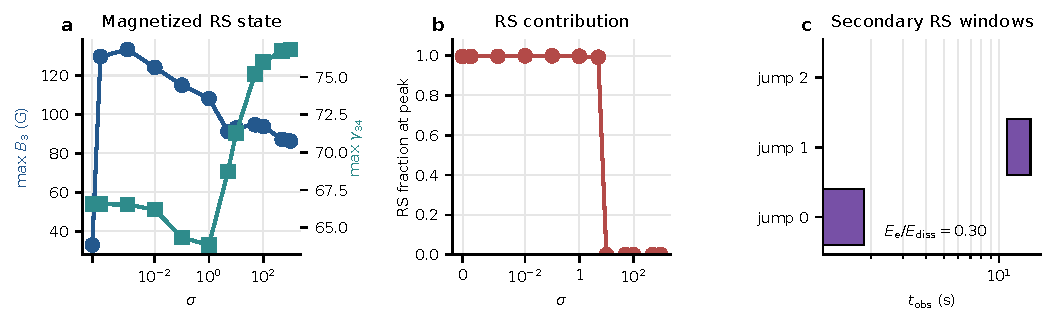
\includegraphics[width=\textwidth]{figures/fig4_reverse_shock.pdf}
  \caption{
\gptareaderanchor{gpta-seg-000383}%
反向激波及密度跃变次级诊断。 (a) 磁化反向激波状态记录为上游 \(\sigma\) 的函数。 (b) 光学峰值处的反向激波通量分数给出了分量贡献。 (c) 根据返回的分支态计算密度跃变次级反向激波事件窗口和注入能量与耗散能量之比。}
  \label{fig:reverse-shock}
\end{figure*}

\section{强子与电子对反馈边界} \label{sec:hadronic}

\subsection{一维激活边界}

\subsubsection{活动物理边界}


\gptareaderanchor{gpta-seg-000384}%
强子输运是一维壳层分支。在前向激波反馈路径中，只有当强子模块启用且质子能量分数 \(\epsilon_p\) 为正时，该分支才被激活。该活跃分支在与前向激波电子和光子相同的半径网格上演化质子、可选次级粒子以及光子存活因子。正式反馈状态为壳层平均。非一维前向电子求解器不被接受，因为ASGARD未针对该分支定义 \(\chi\)-局域靶光子、强子密度或次级反馈。

\subsubsection{受支持强子分支}


\gptareaderanchor{gpta-seg-000385}%
支持的状态分支决定了哪些物理算符进入壳层状态。传统分支仅传输质子并计算质子同步辐射。正式的AM3/Hummer分支增加了\(p\gamma\)相互作用、中微子产生、贝特-海特勒对产生、强子逆康普顿发射、\(pp\)相互作用、次级粒子以及电子对产生反馈\citep{Murase2007,Hummer2010,KelnerAharonian2008,Chodorowski1992,GouldSchreder1967,IceCube2017GRBNeutrinos,Sahu2022GRB190829AHadronic,Sahu2024GRB221009AHadronic}。在观测者整合前，非激活开关会移除相应的算符。返回的状态中缺少不支持的信道。

\subsection{强子 ABI 边界}

\subsubsection{包绑定}


\gptareaderanchor{gpta-seg-000386}%
强子包初始化程序仅选择已编译的内核。它是一个ABI边界，而非粒子输运模型。它定义了两个句柄，
\begin{equation}
\begin{aligned}
H_{\rm FS}&\equiv\texttt{hadronic\_forward\_1d},\\
H_{\rm RS}&\equiv\texttt{hadronic\_reverse\_1d},
\end{aligned}
\end{equation}

\gptareaderanchor{gpta-seg-000387}%
并将公共名称 \texttt{hadronic\_1d} 和 \texttt{reverse\_hadronic\_1d} 分别映射至 \(H_{\rm FS}\) 和 \(H_{\rm RS}\)。该层不改变物理内容。粒子方程、相互作用率和反馈项均在选定的一维核内定义。

\subsection{强子基础网格}

\subsubsection{对数洛伦兹因子网格}


\gptareaderanchor{gpta-seg-000388}%
强子基础网格将粒子谱存储在对数洛伦兹因子网格上。所有过程内核均使用电子、质子、中子、带电π介子、中性π介子和μ子的相同静止质量。这使加速、冷却、衰变和辐射速率统一在同一质量标度上。强子坐标是
\begin{equation}
\begin{aligned}
\Delta x&=\frac{x_{\max}-x_{\min}}{N_\gamma-1},\\
x_i&=x_{\min}+(i-1)\Delta x,\\
\gamma_i&=10^{x_i}.
\end{aligned}
\end{equation}

\gptareaderanchor{gpta-seg-000389}%
这里 \(x_i=\log_{10}\gamma_i\), \(x_{\min}=\log_{10}\gamma_{\min}\),
\(x_{\max}=\log_{10}\gamma_{\max}\), \(\gamma_{\min}>1\)，且
\(\gamma_{\max}>\gamma_{\min}\)。该强子网格与自然对数电子连续性网格是分开的。源项仅作用于强子网格中被允许的部分。其支持存储为
\begin{equation}
\begin{aligned}
i_{\rm L}&=\min\{i\mid \gamma_i\ge\gamma_{\min}^{\rm src}\},\\
i_{\rm H}&=\max\{i\mid \gamma_i\le\gamma_{\max}^{\rm src}\}.
\end{aligned}
\end{equation}

\gptareaderanchor{gpta-seg-000390}%
这两个指数定义了主动注入或相互作用范围。它们不会改变全局传输网格。

\subsubsection{单元面与壳层时间}


\gptareaderanchor{gpta-seg-000391}%
强子输运使用相邻洛伦兹因子中心之间的几何面。对于内部面，
\begin{equation}
\begin{aligned}
\gamma_{i+1/2}=\sqrt{\gamma_i\gamma_{i+1}},
\end{aligned}
\end{equation}
两个边界面为
\begin{equation}
\begin{aligned}
\gamma_{1/2}=\gamma_1\sqrt{\gamma_1/\gamma_2},\qquad
\gamma_{N_\gamma+1/2}=\gamma_{N_\gamma}
\sqrt{\gamma_{N_\gamma}/\gamma_{N_\gamma-1}}.
\end{aligned}
\end{equation}

\gptareaderanchor{gpta-seg-000392}%
\(N_\gamma=1\) 模式是一种低级诊断路径，不用于正式输运分支。每个壳层还需一个正共动时间步长：
\begin{equation}
\begin{aligned}
\Delta t_i' =
\begin{cases}
t'_1, & i=1,\\
t'_i-t'_{i-1}, & i>1,
\end{cases}
\end{aligned}
\end{equation}

\gptareaderanchor{gpta-seg-000393}%
with \(\Delta t_i'>0\)。时间 \(t'_i\) 来自存储的按半径排序的壳层状态，而非来自拟合的观测者网格。基础模块所使用的共动动力学时间为
\begin{equation}
\begin{aligned}
t'_{\rm dyn}=\frac{R}{\Gamma c}.
\end{aligned}
\end{equation}

\subsubsection{遗留最大能量估计}


\gptareaderanchor{gpta-seg-000394}%
传统的质子上限将加速时间与动力学时间和同步辐射冷却进行比较。加速时间与 \(\eta_{\rm acc}\) 成正比，因此较小的 \(\eta_{\rm acc}\) 意味着更快的加速。将加速时间与 \(t'_{\rm dyn}\) 和质子同步辐射冷却时间相等，可得
\begin{equation}
\begin{aligned}
\gamma_{\rm dyn}
&=\frac{eB't'_{\rm dyn}}{\eta_{\rm acc}m_pc},\\
\gamma_{\rm syn}
&=\frac{m_p}{m_e}
\left(\frac{6\pi e}{\eta_{\rm acc}\sigma_{\rm es}B'}\right)^{1/2},\\
\gamma_{\max}=\min(\gamma_{\rm dyn},\gamma_{\rm syn}) .
\end{aligned}
\end{equation}

\gptareaderanchor{gpta-seg-000395}%
这里\(B'\)是共动磁场，\(m_p\)和\(m_e\)分别是质子和电子的质量，\(\sigma_{\rm es}\)是电子散射截面。其他强子核使用相同的基础模块，并要求正的、严格递增的、对数均匀的能量网格。

\subsection{量子同步辐射辅助器}

\subsubsection{QED 不变量}


\gptareaderanchor{gpta-seg-000396}%
量子同步加速辅助器仅改变同步加速冷却速率。它衡量一个带电粒子接近QED同步加速区域的接近程度。对于质量为\(m_s\)的粒子，定义
\begin{equation}
\begin{aligned}
B_Q&=\frac{m_e^2c^3}{e\hbar},&
\hbar&=\frac{h}{2\pi},\\
\chi&=\gamma\,\frac{B'}{B_Q}\,\frac{m_e}{m_s}.
\end{aligned}
\end{equation}

\gptareaderanchor{gpta-seg-000397}%
这里 \(B_Q\) 是电子临界场，\(B'\) 是局域共动场，而 \(\gamma\) 是粒子洛伦兹因子。该辅助函数返回倍增因子。
\begin{equation}
\begin{aligned}
f_q(\gamma,B',m_s)=\mathcal{Q}(\chi).
\end{aligned}
\end{equation}

\gptareaderanchor{gpta-seg-000398}%
强子冷却和辐射辅助工具也采用了这一定义。

\subsubsection{冷却抑制因子}


\gptareaderanchor{gpta-seg-000399}%
冷却因子有一个经典分支和一个量子抑制分支。所实现的AM3风格朗道因子是
\begin{equation}
\mathcal{Q}(\chi)=
\begin{cases}
1, & \chi\le\chi_Q,\\
\left[1+\sqrt{2}\,\chi^{2/3}\right]^{-2}, & \chi>\chi_Q,
\end{cases}
\end{equation}

\gptareaderanchor{gpta-seg-000400}%
其中 \(\chi_Q\) 是小\(\chi\)评估开关。如果 \(B'\le0\) 或 \(\gamma\le1\)，辅助函数返回 \(f_q=1\)。如果量子同步辐射选项被禁用，损失率也保持 \(f_q=1\)。因此，只有当所选运行进入量子同步辐射状态时，辅助函数才会降低经典同步辐射损失率 \citep{Klinger2024AM3}。

\subsection{强子粒子种状态}

\subsubsection{返回的粒子种状态}


\gptareaderanchor{gpta-seg-000401}%
活跃的强子分支返回粒子谱和二次源项。正式的壳层状态是
\begin{equation}
\begin{aligned}
{\cal Y}_h=\{&
N_p,N_n,N_{\pi^0},N_{\pi^\pm},N_{\mu^\pm},\\
&N_\nu,Q_e^{\rm BH},Q_e^{pp},Q_e^{\gamma\gamma}\}.
\end{aligned}
\end{equation}

\gptareaderanchor{gpta-seg-000402}%
这里 \(N_p\) 表示质子谱，\(N_n\) 表示中子谱，\(N_\pi\) 和 \(N_\mu\) 分别为π介子和μ子谱，\(N_\nu\) 为中微子输出，\(Q_e\) 项表示来自贝特-海特勒（Bethe–Heitler）、\(pp\) 及电子对产生通道的正负电子源谱。这些数组是壳层局域的。它们仅通过靶光子场、光子存活因子以及传回电子层的次级对源与辐射耦合。

\subsection{质子过程算子方程}


\gptareaderanchor{gpta-seg-000403}%
质子方程包含了注入、连续损失、相互作用损失以及重子再注入。在紧凑的半径有序形式中，
\begin{equation}
\begin{aligned}
\frac{\partial N_p}{\partial R}
&=Q_{p,R}
+\mathcal{R}_{p\gamma}
-\mathcal{L}_{p\gamma}
-\mathcal{L}_{\rm BH}
-\mathcal{L}_{pp}
-\mathcal{L}_{p,{\rm c}},
\end{aligned}
\end{equation}

\gptareaderanchor{gpta-seg-000404}%
其中\(Q_{p,R}\)是质子源，\(\mathcal{R}_{p\gamma}\)是来自光强子响应的核子重新注入，\(\mathcal{L}_{p\gamma}\)是光强子损失，\(\mathcal{L}_{\rm BH}\)是贝特-海特勒损失，\(\mathcal{L}_{pp}\)是强子核损失，而\(\mathcal{L}_{p,{\rm c}}\)包含连续的绝热损失和质子同步辐射损失。这是一个紧凑的算子表述。每一项都是一个单独的壳层算子，非活动开关在观测者组装之前移除相应的算子。

\subsection{强子粒子种标识符}

\subsubsection{质量与电荷映射}


\gptareaderanchor{gpta-seg-000405}%
加速辅助器只需要粒子的质量和电荷。对于支持的强子和轻子次级，它使用
\begin{equation}
\begin{aligned}
(m_s,Z_s)&\in
\{(m_p,1),(m_n,0),(m_\pi,\pm1),(m_\mu,\pm1)\},\\
|q_s|&=|Z_s|e .
\end{aligned}
\end{equation}

\gptareaderanchor{gpta-seg-000406}%
此处 \(m_s\) 是静止质量，\(Z_s\) 是电荷数，\(q_s\) 是电荷量。中性粒子不参与加速极限计算，因为 \(q_s=0\)。

\subsection{强子壳层能量预算}


\gptareaderanchor{gpta-seg-000407}%
强子源由分配给一个壳层的能量进行归一化。输运核接收该壳层能量为\(E_{s,i}\)。然后它形成
\begin{equation}
\begin{aligned}
L'_{s,i}&=\frac{E_{s,i}}{\Delta t'_i},&
\Delta V_i&=\frac{4\pi}{3}(R_i^3-R_{i-1}^3),
\end{aligned}
\end{equation}

\gptareaderanchor{gpta-seg-000408}%
with \(R_0=0\)。这里，\(L'_{s,i}\) 是形式壳层分支所使用的同移源光度，而 \(\Delta V_i\) 将粒子含量转换为相互作用速率的密度。强子核不通过新的扫过质量公式推断 \(E_{s,i}\)，而是使用上游动力学和运行时配置提供的壳层能量。

\subsection{强子注入谱}


\gptareaderanchor{gpta-seg-000409}%
强子注入谱给出了归一化前的形状。对于物种\(s\)，定义可选截止因子。
\begin{equation}
\begin{aligned}
\mathcal C_s(\gamma)&=
\begin{cases}
\exp(-\gamma/\gamma_{\rm cut}),& {\rm cutoff\ active},\\
1,& {\rm cutoff\ inactive},
\end{cases}
\end{aligned}
\end{equation}
并将未归一化形状写为
\begin{equation}
\begin{aligned}
S_s(\gamma)=
\begin{cases}
\gamma^{-p_s}\mathcal C_s(\gamma),&
\gamma_{\min}\le\gamma\le\gamma_{\rm inj},\\
0, & \gamma<\gamma_{\min}\ {\rm or}\ \gamma>\gamma_{\rm inj},
\end{cases}
\end{aligned}
\end{equation}

\gptareaderanchor{gpta-seg-000410}%
其中，\(p_s\)是注入指数，\(\gamma_{\rm inj}\)是注入粒子的上支撑点。对于前向激波质子，其下支撑点为\(\max(\gamma_{\min},\Gamma)\)，因此注入谱不会从当前体洛伦兹因子以下开始。

\subsection{强子源归一化}


\gptareaderanchor{gpta-seg-000411}%
正式的壳层源使用相对论性能量矩。该矩和归一化源是
\begin{equation}
\begin{aligned}
A_s&=\int S_s(\gamma)\gamma\,d\gamma,\\
Q_s(\gamma)=
\frac{L'_{s,i}S_s(\gamma)}{m_sc^2A_s}.
\end{aligned}
\end{equation}

\gptareaderanchor{gpta-seg-000412}%
此归一化确保了
\(m_sc^2\int Q_s(\gamma)\gamma\,d\gamma=L'_{s,i}\)。该积分在相同的洛伦兹因子网格上计算，注入的壳层内容为
\(Q_s\Delta t'_i\)。仅质子的传统分支采用相同的幂律支撑，但通过动能矩
\(\int S_p(\gamma)(\gamma-1)m_pc^2\,d\gamma\)对壳层内容进行归一化。两个分支均在其各自的源约定中守恒所声明的壳层能量。

\subsection{强子加速极限}


\gptareaderanchor{gpta-seg-000413}%
上限洛伦兹因子通过比较加速时间与动力学时间和同步辐射时间来确定。对于带电粒子，加速时间和同步辐射时间
\begin{equation}
\begin{aligned}
t'_{\rm acc}
&=\eta_{\rm acc}\frac{\gamma m_sc}{|q_s|B'},\\
t'_{\rm syn}
&=\frac{6\pi m_s^3c}
{\sigma_{\rm es}m_e^2B'^2\gamma},
\end{aligned}
\end{equation}

\gptareaderanchor{gpta-seg-000414}%
以及 \(t'_{\rm dyn}=R/(\Gamma c)\)。令 \(t'_{\rm acc}\) 与动力学时间和同步辐射时间相等，得到
\begin{equation}
\begin{aligned}
\gamma_{\rm dyn}
&=\frac{|q_s|B'R}{\eta_{\rm acc}\Gamma m_sc^2},\\
\gamma_{\rm syn}
&=\left[\frac{6\pi |q_s|m_s^2}
{\eta_{\rm acc}\sigma_{\rm es}m_e^2B'}\right]^{1/2}.
\end{aligned}
\end{equation}

\gptareaderanchor{gpta-seg-000415}%
这里 \(\eta_{\rm acc}\) 是加速参数，\(B'\) 是同动磁场，\(\sigma_{\rm es}\) 是电子散射截面。中性粒子不经过此加速极限计算。

\subsection{外部强子冷却极限}


\gptareaderanchor{gpta-seg-000416}%
外部冷却表可以增加一个额外的上能界。如果提供了这样的表，定义正冷却速率 \(\mathcal{C}_{{\rm ext},i}\equiv -(d\gamma/dt')_{\rm ext}|_{\gamma_i}>0\)。对应的冷却时间为
\begin{equation}
\begin{aligned}
t'_{\rm ext}(\gamma_i)=\frac{\gamma_i}{\mathcal{C}_{{\rm ext},i}},
\end{aligned}
\end{equation}

\gptareaderanchor{gpta-seg-000417}%
而 \(t'_{\rm acc}\) 与 \(t'_{\rm ext}\) 的交点给出 \(\gamma_{\rm ext}\)。该交点通过在所提供的网格上对 \(\ln(t'_{\rm acc}/t'_{\rm ext})\) 相对于 \(\ln\gamma\) 进行线性插值得到。所接受的上限为
\begin{equation}
\begin{aligned}
\gamma_{\max}=
\begin{cases}
\min(\gamma_{\rm dyn},\gamma_{\rm syn},\gamma_{\rm ext}),&
\gamma_{\rm ext}\ {\rm exists},\\
\min(\gamma_{\rm dyn},\gamma_{\rm syn}),&
\gamma_{\rm ext}\ {\rm is\ absent}.
\end{cases}
\end{aligned}
\end{equation}

\gptareaderanchor{gpta-seg-000418}%
这个界限设置了活跃强子源所使用的物种网格的顶部。

\subsection{Bethe--Heitler 对产生核}

\subsubsection{运动学变量与阈值}


\gptareaderanchor{gpta-seg-000419}%
Bethe–Heitler分支描述了\(p\gamma\to pe^+e^-\)对产生。对于质子能量\(E_p\)、靶光子能量\(\epsilon\)和次级轻子能量\(E_e\)，该分支首先形成
\begin{equation}
\begin{aligned}
\gamma_p&\equiv \frac{E_p}{m_pc^2},\\
x_\gamma&\equiv \frac{\epsilon}{m_ec^2},\\
x_e&\equiv \frac{E_e}{m_ec^2}.
\end{aligned}
\end{equation}

\gptareaderanchor{gpta-seg-000420}%
这里 \(m_p\) 和 \(m_e\) 分别是质子和电子的质量。只有当质子参照系中的光子能量足够高以产生一对粒子时，该相互作用才被允许，即 \(\gamma_p x_\gamma > 1\)。低于此阈值的网格单元不添加对源、不产生光子汇，也不导致Bethe--Heitler质子损失。

\subsubsection{微分对产生核}


\gptareaderanchor{gpta-seg-000421}%
微分对核给出了单个质子-光子单元中在一个轻子能量下的对产额。对于允许的单元，ASGARD在质子系光子能量\(\omega\)和中间轻子能量\(\bar E\)上积分Blumenthal–Gould Bethe–Heitler截面\citep{BlumenthalGould1970}：
\begin{equation}
\begin{aligned}
C_{\rm BH}&\equiv \frac{x_e}{2\gamma_p^3x_\gamma^2},\\
I_{\rm BH}
&\equiv \int_{\omega_{\min}}^{\omega_{\max}} d\omega
\int_{\bar E_{\min}}^{\omega-1} d\bar E\,
\frac{\omega\,\sigma_{\rm BH}(\omega,\bar E,\xi)}{\bar p},\\
\mathcal{K}_{\rm BH}(x_e,\gamma_p,x_\gamma)
&\equiv C_{\rm BH}I_{\rm BH}.
\end{aligned}
\end{equation}

\gptareaderanchor{gpta-seg-000422}%
前因子\(C_{\rm BH}\)将积分转换为所选的轻子能量变量，而\(\mathcal{K}_{\rm BH}\)是源项和损失项求和所用的网格核函数。积分限和局域角变量为
\begin{equation}
\begin{aligned}
\omega_{\max}&=2\gamma_px_\gamma,\\
\omega_{\min}&=\frac{(\gamma_p+x_e)^2}{2\gamma_px_e},\\
\bar E_{\min}&=\frac{\gamma_p^2+x_e^2}{2\gamma_px_e},\\
\bar p&=(\bar E^2-1)^{1/2},\\
\xi&=\frac{\gamma_p\bar E-x_e}{\gamma_p\bar p}.
\end{aligned}
\end{equation}

\gptareaderanchor{gpta-seg-000423}%
如果下限达到上限，则配对相空间封闭，且\(\mathcal{K}_{\rm BH}=0\)。

\subsubsection{拟合域与求积控制}


\gptareaderanchor{gpta-seg-000424}%
Bethe–Heitler截面拟合具有有限的光子能量范围。ASGARD仅在\(\omega_{\rm BH,L}<\omega<\omega_{\rm BH,H}\)范围内评估\(\sigma_{\rm BH}\)，在此拟合窗口之外，微分核为零。下界是电子对产生阈值，上界是所采用解析拟合的有限域。两个积分通过固定的求积控制参数\(N_\omega\)和\(N_{\bar E}\)进行计算，这些参数决定了在\(\omega\)和\(\bar E\)方向上的分辨率。

\subsubsection{次级电子对源}


\gptareaderanchor{gpta-seg-000425}%
次级对源将Bethe--Heitler轻子添加到电子和正电子网格中。在对数均匀的质子和光子网格上，ASGARD写入
\begin{equation}
\begin{aligned}
Y_i&\equiv E_{p,i}N_p(E_{p,i}),\\
Z_k&\equiv \epsilon_k n_\gamma(\epsilon_k),\\
K_{jik}&\equiv
\mathcal{K}_{\rm BH}(x_{e,j},\gamma_{p,i},x_{\gamma,k}),\\
k_{\rm BH}&\equiv \frac{3c\sigma_{\rm es}\alpha_{\rm f}}{16\pi},\\
Q_e^{\rm BH}(E_{e,j})
&=\frac{k_{\rm BH}\Delta\ln E_p\,\Delta\ln\epsilon}{E_{e,j}}
\sum_{i,k}Y_iZ_kK_{jik}.
\end{aligned}
\end{equation}

\gptareaderanchor{gpta-seg-000426}%
这里 \(N_p\) 是质子谱，\(n_\gamma\) 是靶光子密度，\(\alpha_{\rm f}\) 是精细结构常数，而 \(\sigma_{\rm es}\) 是电子散射截面。输出 \(Q_e^{\rm BH}\) 是一个壳层局部的每轻子能量 \(e^\pm\) 注入率。

\subsubsection{靶光子汇}


\gptareaderanchor{gpta-seg-000427}%
目标光子汇移除参与相同Bethe--Heitler相互作用的光子。对于每个光子箱，
\begin{equation}
\begin{aligned}
D_k&\equiv \epsilon_k n_\gamma(\epsilon_k),\\
\Lambda_{\gamma}^{\rm BH}(\epsilon_k)
&=\frac{k_{\rm BH}\Delta\ln E_p\,\Delta\ln E_e}{D_k}
\sum_{i,j}Y_iZ_kK_{jik}.
\end{aligned}
\end{equation}

\gptareaderanchor{gpta-seg-000428}%
正比 \(\Lambda_{\gamma}^{\rm BH}\) 随后转换为壳层单元的光学深度和相应的光子存活因子。
如果 bin \(k\) 中的目标光子密度为零，则该 bin 中的光子损失率设为零。

\subsubsection{质子冷却率}


\gptareaderanchor{gpta-seg-000429}%
质子冷却速率记录了质子在与贝特-海特勒相互作用中损失的能量。ASGARD使用Chodorowski等人的能量损失核\(\phi_{\rm C}\) \citep{Chodorowski1992}，并将正冷却速率写为
\begin{equation}
\begin{aligned}
\Phi_k^{\rm C}
&\equiv \frac{\phi_{\rm C}(2\gamma_px_{\gamma,k})}
{2\gamma_p^2x_{\gamma,k}^2},\\
k_{p{\rm BH}}&\equiv
\frac{3\alpha_{\rm f}\sigma_{\rm es}c}{8\pi}\frac{m_e}{m_p},\\
\mathcal{C}_p^{\rm BH}(\gamma_p)
&\equiv -\left(\frac{d\gamma_p}{dt'}\right)_{\rm BH}\\
&=k_{p{\rm BH}}\Delta\ln\epsilon
\sum_k\Phi_k^{\rm C}Z_k.
\end{aligned}
\end{equation}

\gptareaderanchor{gpta-seg-000430}%
速率 \(\mathcal{C}_p^{\rm BH}\) 作为损失项进入质子输运方程。

\subsubsection{Chodorowski 损失拟合}


\gptareaderanchor{gpta-seg-000431}%
损失核使用Chodorowski等人的分段拟合。当 \(x_{\rm th}=2\) 时，拟合函数为
\begin{equation}
\phi_{\rm C}(x)=
\begin{cases}
0, & x<x_{\rm th},\\
\Phi_{\rm L}(x;\mathbf{a}_{\rm C}), & x_{\rm th}\le x<x_{\rm C},\\
\Phi_{\rm H}(x;\mathbf{b}_{\rm C}), & x\ge x_{\rm C},
\end{cases}
\end{equation}

\gptareaderanchor{gpta-seg-000432}%
其中 \(x_{\rm C}\) 是低能分支与高能分支之间的匹配点。系数集 \(\mathbf{a}_{\rm C}\) 和 \(\mathbf{b}_{\rm C}\) 是已发表的拟合参数。因此，贝特-海特勒分支返回三个壳层局域量：一个次级 \(e^\pm\) 源、一个正质子冷却率 \(\mathcal{C}_p^{\rm BH}\)，以及一个正靶光子损失率 \(\Lambda_{\gamma}^{\rm BH}\)。

\subsection{质子输运算子}

\subsubsection{\texorpdfstring{Log-\(\gamma_p\)}{Log-gamma-p} 输运步骤}


\gptareaderanchor{gpta-seg-000433}%
质子输运算子在推进次级粒子之前，将注入的壳层质子经历冷却和强子相互作用。谱被存储在强子 \(\log_{10}\gamma_p\) 网格上。冷却将粒子含量从高 \(\gamma_p\) 移动到低 \(\gamma_p\)，因此所有连续损失都写为正速率。
\begin{equation}
\begin{aligned}
C_p(\gamma_p)&\equiv
-\left(\frac{d\gamma_p}{dt'}\right)_{\rm loss},\\
\frac{\partial N_p}{\partial t'}
&-\frac{\partial}{\partial\gamma_p}
\left(C_pN_p\right)
=Q_p+Q_{p,{\rm r}} .
\end{aligned}
\end{equation}

\gptareaderanchor{gpta-seg-000434}%
这里 \(N_p=dN_p/d\gamma_p\)，\(Q_p\) 是初级质子源，而 \(Q_{p,{\rm r}}\) 是由 \(p\gamma\) 响应返回的质子源。在正式反馈分支中，该方程的连续部分通过单元内容的保守重映射进行评估。对于时间步长 \(\Delta t'\)，
\begin{equation}
\begin{aligned}
C_i^{\rm c} &=
C_{\rm ad,i}+C_{{\rm syn},i}+C_{{\rm BH},i}+C_{{\rm pp},i},\\
\gamma_i^{\rm c} &= \gamma_i-C_i^{\rm c}\Delta t',\\
\Delta N_i &= N_{p,i}\Delta\gamma_i,\\
N_{p,a}^{\rm c} &=
\frac{1}{\Delta\gamma_a}
\sum_{\gamma_i^{\rm c}\in[\gamma_{a-1/2},\gamma_{a+1/2})}\Delta N_i
+\mathcal{Q}_{p,a}.
\end{aligned}
\end{equation}

\gptareaderanchor{gpta-seg-000435}%
这里\(C_i^{\rm c}\)是质子细胞\(i\)中的连续冷却速率，\(\gamma_i^{\rm c}\)是冷却后的细胞中心，\(\mathcal{Q}_{p,a}\)是在同一壳层步骤中注入的质子含量。在存储网格外部冷却的内容不会被分配到网格细胞。原有的仅质子分支使用相同守恒定律的上风流形式；它不是用于耦合电子-光子-强子运行的形式反馈路径。

\subsubsection{基线质子损失}


\gptareaderanchor{gpta-seg-000436}%
基线质子损失是绝热冷却和质子同步加速冷却。在添加任何碰撞算子之前，代码使用
\begin{equation}
\begin{aligned}
C_{\rm ad}(\gamma_p)&=\frac{\gamma_p}{t'_{\rm dyn}},\\
C_{\rm syn}&=
\frac{\sigma_{\rm es} B'^2}{6\pi m_ec}
\left(\frac{m_e}{m_p}\right)^3\gamma_p^2.
\end{aligned}
\end{equation}

\gptareaderanchor{gpta-seg-000437}%
这里 \(t'_{\rm dyn}\) 是同动壳层膨胀时间，而 \(B'\) 是同动磁场。Bethe--Heitler 损失和 \(pp\) 损失仅在它们的分支活跃时才被添加到连续速率 \(C_i^{\rm c}\) 中。\(p\gamma\) 损失在重映射后被处理为一个指数相互作用汇，并伴有同一步长的再注入源，
\begin{equation}
\begin{aligned}
\tau_{p\gamma,i} &= \lambda_{p\gamma,i}\Delta t',\\
t'_{{\rm eff},i} &=
\begin{cases}
\left(1-e^{-\tau_{p\gamma,i}}\right)/\lambda_{p\gamma,i},
& \lambda_{p\gamma,i}>0,\\
\Delta t',&\lambda_{p\gamma,i}=0,
\end{cases}\\
N_{p,i}^{\rm new} &=
N_{p,i}^{\rm c}e^{-\tau_{p\gamma,i}}
+t'_{{\rm eff},i}V_i\mathcal{R}_{p\gamma,i}.
\end{aligned}
\end{equation}

\gptareaderanchor{gpta-seg-000438}%
此处 \(\lambda_{p\gamma,i}\) 为正质子相互作用率，\(V_i\) 为壳层体积，\(\mathcal{R}_{p\gamma,i}\) 为经过壳层算子使用的代码单位转换后的再注入源。该步骤将丢失和再注入的质子含量保持在相同的壳层更新中。

\subsection{\texorpdfstring{\(p\gamma\)}{p-gamma} 壳层生存算子}


\gptareaderanchor{gpta-seg-000439}%
\(p\gamma\)幸存算子描述了强子响应，即哪些目标光子保留在一个壳层单元中。ASGARD使用两次通过。第一次通过作用于未衰减的光子密度，并返回光子损失深度。第二次通过作用于幸存的光子场，并返回相互作用率、次级产额和\(Q_{p,{\rm r}}\)。对于\(\tau_g\equiv\tau_\gamma(\nu',R)\)，有限单元幸存因子为
\begin{equation}
S_\gamma(\nu',R)=
\frac{1-e^{-\tau_g}}{\tau_g},
\end{equation}

\gptareaderanchor{gpta-seg-000440}%
当\(\tau_g\rightarrow0\)时，有\(S_\gamma\rightarrow1\)。该因子是第二次通过时所看到的经单元平均的光子密度。返回的光子存活数组随后被应用于质子同步辐射、次级同步辐射、中性π介子光子、贝特-海特勒光子、强子逆康普顿光子以及π介子/μ子辐射，然后再进行观测者投影。该分支是壳层局域且一维的。

\subsection{次级粒子种源算子}


\gptareaderanchor{gpta-seg-000441}%
次级物种源算符将强子相互作用转化为局部粒子源项。这些输运的次级物种仅在形式一维路径中得到支持。

\subsubsection{\texorpdfstring{\(p\gamma\)}{p-gamma} 响应产物}


\gptareaderanchor{gpta-seg-000442}%
\(p\gamma\) 响应产物是在应用目标光子存活后产生的粒子。存活场响应产生中性π介子伽马射线、带电π介子、μ子、中微子、中子重注入和质子重注入。这些产物是观察者投影前的局部壳层输出；如果没有单独的曝光计算，中微子阵列不被解释为探测预测。

\subsubsection{\texorpdfstring{\(pp\)}{pp} delta 源}


\gptareaderanchor{gpta-seg-000443}%
当重子壳靶处于激活状态时，\(pp\)源算子提供紧凑型π介子源。该分支采用带有固定参数集的δ近似。
\begin{equation}
\left(\kappa_{pp},\xi_\pi,f_{\pi^0}\right),
\end{equation}

\gptareaderanchor{gpta-seg-000444}%
其中\(\kappa_{pp}\)为非弹性度，\(\xi_\pi\)为π介子能量分数，\(f_{\pi^0}\)为中性π介子分数。输出是一个局部次级源，而非独立的辐射成分。

\subsubsection{Bethe--Heitler 电子对交接}


\gptareaderanchor{gpta-seg-000445}%
Bethe--Heitler交接告诉代码在哪里计数产生的对。
Bethe--Heitler对和\(pp\)对作为次级电子源被累积。
在分离分支中，Bethe--Heitler次级电子可以合并到前向电子分布中。
在这种情况下，单独的Bethe--Heitler光度不会被组合，因此相同的注入能量在一个地方被计数。

\subsection{联合电子--光子--强子反馈迭代}

\subsubsection{局部不动点序列}


\gptareaderanchor{gpta-seg-000446}%
联合反馈分支在观测者投影前更新一个壳层内的电子、光子和强子。一次局部迭代的顺序为
\begin{equation}
\begin{aligned}
N_e^{(r)}
&\rightarrow n_\gamma^{(r)}
\rightarrow
\left\{Q_e^{{\rm sec},(r)},\tau_{\gamma\gamma}^{(r)}\right\}
\rightarrow N_e^{(r+1)}.
\end{aligned}
\end{equation}

\gptareaderanchor{gpta-seg-000447}%
这里 \(r\) 是局部迭代索引。次级源进入 \(Q_e^{\rm sec}\)，更新后的电子解重建光子场，并在幸存的目标场上重新评估强子算子。观测者计算只看到此局部序列完成后的状态。

\subsubsection{级联分支边界}


\gptareaderanchor{gpta-seg-000448}%
级联边界规定了所支持的电磁反馈路径。
当请求的级联次数满足\(N_{\rm cas}>1\)时，ASGARD使用
壳层序列时变\(\gamma\gamma\)对/同步加速级联路径。
单壳层路径是一种诊断模式，该分支不实现
逆康普顿介导的电磁级联。

\subsection{壳层序列电子对级联算法}

\subsubsection{电子对网格与逃逸时间}


\gptareaderanchor{gpta-seg-000449}%
壳层序列级联是受支持的时变电磁级联分支。它将成对粒子从一个径向壳层携带到下一个壳层，并在观测者投影前更新每个壳层内的局部光子密度。计算首先将种子光子场写为 \(n_\epsilon=dN_\gamma/d\epsilon\)，然后将成对粒子置于与光子网格具有相同对数间隔的能量网格上。
\begin{equation}
\begin{aligned}
j_0&=\left\lceil
\frac{\ln(m_ec^2/E_{\gamma,1})}{\Delta\ln E}
\right\rceil,\\
E_{e,j}&=E_{\gamma,1}\exp[(j-1+j_0)\Delta\ln E],\\
\gamma_{e,j}&=\frac{E_{e,j}}{m_ec^2}.
\end{aligned}
\end{equation}

\gptareaderanchor{gpta-seg-000450}%
其中 \(E_{\gamma,1}\) 是第一个光子箱的能量，\(\Delta\ln E\) 是共同对数间距，\(j_0\) 是使第一个对子箱位于或高于 \(m_ec^2\) 的整数偏移。在层 \(i\) 中，光子在逃逸时间内保留在网格内。
\begin{equation}
t'_{{\rm esc},i}=\frac{R_i}{\eta_{\rm esc}\Gamma_i c},
\end{equation}

\gptareaderanchor{gpta-seg-000451}%
其中\(R_i\)和\(\Gamma_i\)分别是壳体半径和洛伦兹因子，\(\eta_{\rm esc}\)是固定的壳体逃逸几何因子。该逃逸时间同时设定了光子驻留时间和用于光子密度更新的源尺度。

\subsubsection{\texorpdfstring{\(\gamma\gamma\)}{gamma-gamma} 源项计算}


\gptareaderanchor{gpta-seg-000452}%
γγ源评估将吸收的光子转化为次级对。在子步骤 \(m\)，当前光子密度被传递给与壳层不透明度计算相同的角度平均对产生算符：
\begin{equation}
n_\epsilon^{(m)}
\rightarrow
\left\{\lambda_{\gamma\gamma}(\epsilon),
q_{\pm,\gamma\gamma}(E_e),P_{\rm abs},P_{\rm inj}\right\},
\end{equation}

\gptareaderanchor{gpta-seg-000453}%
其中\(\lambda_{\gamma\gamma}\)是局部光子损失率，\(q_{\pm,\gamma\gamma}\)是每能量的组合\(e^-+e^+\)注入率，而\(P_{\rm abs}\)和\(P_{\rm inj}\)是用作能量闭合诊断的吸收和注入功率。在一个子步中添加到对\(\gamma\)-网格的源是
\begin{equation}
\begin{aligned}
S_{\pm,j}^{(m)}&=\Delta V_i\,m_ec^2\,
q_{\pm,\gamma\gamma}(E_{e,j})\,\Delta t'_{\rm sub},\\
\Delta t'_{\rm sub}&=\frac{\Delta t'_i}{N_{\rm sub}} .
\end{aligned}
\end{equation}

\gptareaderanchor{gpta-seg-000454}%
这里\(\Delta V_i\)是壳层体积，\(\Delta t'_i\)是同移壳层时间宽度，\(N_{\rm sub}\)是声明的级联子步数。存储的功率\(P_{\rm abs}\)和\(P_{\rm inj}\)是局部诊断量；它们不是观测者系通量。

\subsubsection{有限网格电子对冷却}


\gptareaderanchor{gpta-seg-000455}%
有限网格对冷却步骤将携带的和新注入的对移动到较低的洛伦兹因子。在壳层\(i\)中，正冷却速率是
\begin{equation}
\begin{aligned}
t'_{{\rm dyn},i}&=\frac{R_i}{\Gamma_i c},\\
C_{{\rm syn},i}(\gamma)
&=\frac{\sigma_{\rm es} B_i'^2}{6\pi m_ec}\gamma^2,\\
\mathcal{C}_{\pm,i}(\gamma)
&\equiv -\left(\frac{d\gamma}{dt'}\right)_{\pm,i}\\
&=C_{{\rm syn},i}(\gamma)+\frac{\gamma}{t'_{{\rm dyn},i}}.
\end{aligned}
\end{equation}

\gptareaderanchor{gpta-seg-000456}%
这里 \(t'_{{\rm dyn},i}\) 是共动膨胀时间，\(B_i'\) 是共动磁场。离散更新将格点 \(j\) 中的粒子对含量存储为 \(\Delta N_j=N_j\Delta\gamma_j\)，并将格点中心冷却到
\begin{equation}
\begin{aligned}
\gamma_j^{\rm c}
&=\gamma_j-\mathcal{C}_{\pm,i}(\gamma_j)\Delta t'_{\rm sub},\\
N_j^{(m+1)}
&=
\frac{1}{\Delta\gamma_j}
\sum_{\gamma_\ell^{\rm c}\in[\gamma_{j-1/2},\gamma_{j+1/2})}
\Delta N_\ell^{(m)}
+S_{\pm,j}^{(m)} .
\end{aligned}
\end{equation}

\gptareaderanchor{gpta-seg-000457}%
因此，成对更新是有限网格冷却内容的重映射加上当前的\(\gamma\gamma\)源。如果\(\gamma_j^{\rm c}\)位于有限成对网格之外，则该内容离开所表示的级联种群。

\subsubsection{光子密度传递}


\gptareaderanchor{gpta-seg-000458}%
光子密度传递在一个壳层中闭合了局域电子对-光子循环。更新后的电子对分布被传递给同步辐射状态算符，该算符返回电子对同步辐射光度 \(L_{\nu',\pm}'\) 和局域电子对种子光子密度 \(n_{\nu',\pm}'\)。随后，光子场求解子步方程。
\begin{equation}
\frac{dn_\epsilon}{dt'}=
S_\epsilon-\Lambda_\epsilon n_\epsilon,
\end{equation}
with
\begin{equation}
\begin{aligned}
\Lambda_\epsilon&=\lambda_{\gamma\gamma}(\epsilon)+\frac{1}{t'_{\rm esc}},\\
S_\epsilon&=\frac{n_{\epsilon,{\rm prim}}+n_{\epsilon,\pm}}{t'_{\rm esc}},\\
n_{\epsilon,\pm}&=\frac{n_{\nu',\pm}'}{h},\\
A_\epsilon&=\exp(-\Lambda_\epsilon\Delta t'_{\rm sub}),\\
n_\epsilon^{(m+1)}=
A_\epsilon n_\epsilon^{(m)}
+\frac{S_\epsilon}{\Lambda_\epsilon}(1-A_\epsilon).
\end{aligned}
\end{equation}

\gptareaderanchor{gpta-seg-000459}%
这里 \(n_{\epsilon,{\rm prim}}\) 是原初壳层光子密度，而 \(n_{\epsilon,\pm}\) 是级联对发射的光子密度。记录的局部光学深度为 \(\tau_{\gamma\gamma}=\lambda_{\gamma\gamma}t'_{\rm esc}\)。传递到观测者模块的输出包括每个壳层的对密度、对同步辐射光度、对种子光子密度以及 \(\gamma\gamma\) 光学深度。

\subsection{单壳层电子对同步辐射诊断}

\subsubsection{冷却轨迹}


\gptareaderanchor{gpta-seg-000460}%
单壳诊断是对\(\gamma\gamma\)对同步加速核的局部检查。它在一个光子场中评估对算符，返回光子损失率和吸收功率，然后沿着同步加速冷却路径追踪注入的对。它不会将对携带到下一个壳层，也不会更新壳层光子密度。对于\(B'>0\)，在\(\gamma_i\)处注入的一对在诊断路径时间\(t'_p\)内冷却至
\begin{equation}
\begin{aligned}
a_B&=\frac{\sigma_{\rm es}B'^2}{6\pi m_ec},\\
\gamma_i^{\rm c}&=
\frac{\gamma_i}{1+a_B\gamma_i t'_p},\\
t_{\rm cool}(\gamma)&=\frac{1}{a_B\gamma^2}.
\end{aligned}
\end{equation}

\gptareaderanchor{gpta-seg-000461}%
该诊断将注入的对源 \(q_{\pm,i}^{\rm d}\) 沉积在 \(\gamma_i^{\rm c}\) 和 \(\gamma_i\) 之间的网格单元上。
\begin{equation}
N_{\pm,j}^{\rm d}
=
\sum_{\gamma_i^{\rm c}<\gamma_j\le\gamma_i}
q_{\pm,i}^{\rm d}\,t_{\rm cool}(\gamma_j)\,\Delta\ln\gamma .
\end{equation}

\gptareaderanchor{gpta-seg-000462}%
这里 \(q_{\pm,i}^{\rm d}\) 是由诊断对算符返回的局域对源。如果 \(B'\le0\)，诊断不返回对同步辐射发射率，尽管来自对算符的光子损失率仍然有定义。

\subsubsection{诊断发射率}


\gptareaderanchor{gpta-seg-000463}%
诊断发射率将冷却的诊断对映射到同步辐射光子。它使用
\begin{equation}
\begin{aligned}
C_\nu&=\frac{3e}{4\pi m_ec},\\
\nu_s&=C_\nu B'\gamma^2,
\end{aligned}
\end{equation}
以及单粒子近似
\begin{equation}
\begin{aligned}
P_\nu&\simeq C_PB'\Phi_{\rm d}(\nu/\nu_s),\\
C_P&=\frac{\sqrt{3}e^3}{m_ec^2},\\
\Phi_{\rm d}(x)&=A_{\rm d}x^{1/3}e^{-x}.
\end{aligned}
\end{equation}

\gptareaderanchor{gpta-seg-000464}%
这里 \(A_{\rm d}\) 是诊断发射率核的固定系数。
那么诊断光子谱为
\begin{equation}
L_\nu^{\rm d}
=
\sum_j P_\nu(\gamma_j)N_{\pm,j}^{\rm d}\gamma_j\Delta\ln\gamma .
\end{equation}

\gptareaderanchor{gpta-seg-000465}%
该谱用于检验级联算子的局部同步辐射部分。正式的正负电子对级联输出仍保持上一小节中的壳层序列状态。

\section{观测者投影与分量组装} \label{sec:projection}

\subsection{等到达时间投影}

\subsubsection{局部角向映射}


\gptareaderanchor{gpta-seg-000466}%
观测者投影是计算的最后一步。它读取局域半径排序的光谱和吸收因子，将其映射到等到达时间面，然后将角度单元求和得到\(F_\nu(t_{\rm obs})\)。对于一个位于极角\(\theta\)、方位角\(\phi\)和观测角\(\theta_v\)的角度单元，局域几何是
\begin{equation}
\begin{aligned}
\mu&=\cos\theta_v\cos\theta+\sin\theta_v\sin\theta\cos\phi,\\
t_{\rm arr}(R,\theta,\phi)
&=t_0(R)+\frac{(1+z)R(1-\mu)}{c},\\
\eta_\delta&\equiv\delta^{-1}=\Gamma(1-\beta\mu).
\end{aligned}
\end{equation}

\gptareaderanchor{gpta-seg-000467}%
此处 \(\mu\) 是网格速度与视线方向之间夹角的余弦值，\(t_0(R)\) 是由局部动力学解提供的轴向壳层到达时间，而 \(\eta_\delta\) 是由投影内核存储的逆多普勒因子。此步骤改变了局部光子的观测方式，但并未改变局部粒子或光子的状态。

\subsubsection{半径到观测者插值}


\gptareaderanchor{gpta-seg-000468}%
半径到观测者的插值将每个局部光谱置于观测者时间网格上。沿着等到达时间面，代码计算共动频率和角权重作为
\begin{equation}
\begin{aligned}
\nu'&=\nu_{\rm obs}(1+z)\eta_\delta,\\
dW&=\eta_\delta^{-3}\frac{d\Omega}{4\pi}.
\end{aligned}
\end{equation}

\gptareaderanchor{gpta-seg-000469}%
对于两个相邻到达半径之间的观察者时间点，代码在该径向段内对局部SED进行线性插值。随后，代码在对数网格上对频率进行插值：当两个相邻SED值均为正时使用对数-对数插值，否则使用线性插值。因此，密度跳跃和注入特征仅因等到达时间几何以及上述插值规则而被展宽。

\subsection{结构喷流聚合边界}

\subsubsection{后端选择}


\gptareaderanchor{gpta-seg-000470}%
后端选择指定了哪个角投影路径处于激活状态。一个带有支持介质的直接顶帽模型使用直接核支持路径。结构化喷流通过Fortran结构化后端或Python补丁后端以角补丁形式求解。Fortran结构化后端支持均匀补丁采样以及一维\texttt{fullhide\_1d}或\texttt{dg\_1d}电子求解器。当所需的一维强子响应处于激活状态时，它可处理前向激波同步辐射、前向SSC、反向激波同步辐射以及支持的结构化\(p\gamma\)/中微子路径。该后端不支持反向激波SSC、跨区IC、反向激波强子分支、Bethe-Heitler过程、\(pp\)、强子IC或对级联分支。\texttt{dominant\_region\_ioka\_v1}和\texttt{dominant\_region\_ioka\_time\_v1}采样器使用Python补丁后端。

\subsubsection{活动斑块寄存器}


\gptareaderanchor{gpta-seg-000471}%
主动补丁寄存器告诉结构化后端哪些角细胞被物理求解。Python调用者在中间点细胞上采样射流并传递
\begin{equation}
\begin{aligned}
E_{ab}&=E_{\rm iso}(\phi_b,\theta_a),\\
\Gamma_{0,ab}&=\Gamma_0(\phi_b,\theta_a),\\
I^E_{ab}&=\mathbf{1}(E_{ab}>0),\\
I^\Gamma_{ab}&=\mathbf{1}(\Gamma_{0,ab}\ge\Gamma_{\min}),\\
A_{ab}&=I^E_{ab}I^\Gamma_{ab},
\end{aligned}
\end{equation}

\gptareaderanchor{gpta-seg-000472}%
其中 \(a\) 和 \(b\) 标记极坐标和方位角网格。量 \(\Gamma_{\min}\) 是相对论后端激活边界，而非额外的物理参数。编译后的 \texttt{structured\_jet\_1d} 条目接收活动网格，求解活动补丁的局部一维状态，然后根据每个补丁自身的角权重进行投影。仅当所有活动环共享相同的 \(E_{ab}\) 和 \(\Gamma_{0,ab}\) 时，Python 环路径才能复用已求解的状态；否则，各局部补丁状态将被单独求解。

\subsubsection{局部一维求解}


\gptareaderanchor{gpta-seg-000473}%
局部一维求解与直接顶帽模型使用的物理求解相同。对于活动补丁\(q\)，聚合仅替换局部边界条目。
\begin{equation}
\Gamma_0\leftarrow\Gamma_{0,q},\qquad
E_{\rm iso}\leftarrow E_q
\end{equation}

\gptareaderanchor{gpta-seg-000474}%
然后运行之前描述的一维动力学、电子、可选SSC、反向同步辐射以及选定的强子成分内核。结构化聚合体改变角权重和状态重用。它不改变局部激波、粒子或同步辐射方程。

\subsubsection{壳层前因子}


\gptareaderanchor{gpta-seg-000475}%
壳层前置因子将局部组分光度转化为观测投影仪允许读取的光谱。它首先根据活跃光子场和光学深度构建壳层吸收因子，随后对每个活跃分量应用距离稀释和红移。对于标记为 \(c\) 的分量，
\begin{equation}
\begin{aligned}
\mathcal{P}_{\nu'}(R)&=
\frac{1+z}{4\pi d_L^2}\,
\mathcal{A}_{\rm abs}(\nu',R),\\
\widetilde L_{\nu'}^{\,c}(R,q)=
\mathcal{P}_{\nu'}(R)L_{\nu'}^{\prime c}(R,q).
\end{aligned}
\end{equation}

\gptareaderanchor{gpta-seg-000476}%
这里 \(d_L\) 是光度距离，\(\mathcal{A}_{\rm abs}\) 是在添加额外光学深度后由光子-光子吸收路径返回的综合局部吸收因子。活动标签可以包括 FS-同步辐射、FS-SSC、FS 强子光子、Bethe-Heitler 光子、强子逆康普顿、对级联光子、RS 同步辐射、RS 强子光子、RS-SSC 以及跨区逆康普顿。未活动的组件不会出现在观测者组件列表中。

\subsubsection{角向累积}


\gptareaderanchor{gpta-seg-000477}%
角度累加在每个活动分量在总和中形成之前对其进行投影。轴对称结构轮廓使用\texttt{SED\_interpolation\_structured}，而显式的二维角度网格使用\texttt{sed\_structured\_phi}。直接顶帽路径使用选定的等到达时间插值核。投影后，返回的总和是各分量的代数和。
\begin{equation}
\begin{aligned}
F_{\nu}(t_{\rm obs})&=
F_{\nu}^{\rm FS,syn}
+F_{\nu}^{\rm FS,SSC}
+F_{\nu}^{\rm FS,had}\\
&\quad
+F_{\nu}^{\rm RS,syn}
+F_{\nu}^{\rm RS,had}
+F_{\nu}^{\rm RS,SSC}
+F_{\nu}^{\rm cross}.
\end{aligned}
\end{equation}

\gptareaderanchor{gpta-seg-000478}%
从求和中省略非活动项。通过结构化求解返回的诊断半径轨迹从记录该轨迹的第一个补丁中复制。这是一个局部的一维历史，而不是通量加权角平均。

\subsection{投影符号绑定}


\gptareaderanchor{gpta-seg-000479}%
投影符号绑定仅将Python名称连接到编译后的投影内核。它不是一个辐射模型，也不选择观测者几何。\texttt{src.Interpolation}初始化器将公共名称\texttt{sed\_interpolation}、\texttt{sed\_adaptive\_theta}、\texttt{sed\_interpolation\_chi}、\texttt{sed\_chi\_electron}、\texttt{sed\_chi\_ring}、\texttt{sed\_chiring\_batchlum}和\texttt{sed\_chiring\_batchlum\_ray}映射到编译后的\texttt{SED\_interpolation}模块。首次访问时，它会导入该模块，并将请求的符号复制到包命名空间中。此列表之外的名称不会被导出。因此，该绑定暴露了投影映射
\begin{equation}
\{\widetilde L_{\nu'}(R),\tau_{\nu'}(R),R,\Gamma,t_{\rm obs},\nu_{\rm obs}\}
\longrightarrow F_{\nu_{\rm obs}}(t_{\rm obs}),
\end{equation}

\gptareaderanchor{gpta-seg-000480}%
同时将辐射过程、光学深度、多普勒因子、到达时间图以及插值权重保留在选定的Fortran内核中。

\subsection{直接顶帽等到达时间插值}

\subsubsection{中点角向单元}


\gptareaderanchor{gpta-seg-000481}%
中点角度单元将一个直接顶帽外壳分割成小的发射表面单元。每个单元在半径变化时保持一对角度。直接\texttt{SED\_interpolation}内核利用这些单元构建等到达时间求和。在外壳级路径中，角度单元\(a\)的立体角
\begin{equation}
\Delta\Omega_a=
(\cos\theta_{a,-}-\cos\theta_{a,+})\,\Delta\phi .
\end{equation}

\gptareaderanchor{gpta-seg-000482}%
这里 \(\theta_{a,-}\) 和 \(\theta_{a,+}\) 分别是下极边缘和上极边缘，\(\Delta\phi\) 是方位角宽度。当公共顶帽网格存储了一个折叠的方位角半平面时，代码使用名为折叠网格控制 \(N_{\phi,c}\) 来恢复完整的方位角权重，而不改变局部到达时间图。对于每个角单元，方向余弦和到达时间
\begin{equation}
\begin{aligned}
\mu&=\cos\theta_v\cos\theta+\sin\theta_v\sin\theta\cos\phi ,\\
t_{\rm arr}(R)&=t_0(R)+\frac{(1+z)R(1-\mu)}{c}.
\end{aligned}
\end{equation}

\gptareaderanchor{gpta-seg-000483}%
这里\(\theta\)和\(\phi\)是单元中点角，\(\theta_v\)是视角，\(t_{\rm arr}\)是半径\(R\)对应的观测者到达时间。该角度块的输出是一组单元权重和到达时间轨迹；它不改变存储在半径网格上的局部谱。

\subsubsection{径向到达时间括定}


\gptareaderanchor{gpta-seg-000484}%
径向到达时间区间找到在给定观测者时间、一个角度单元内发射光子的半径。如果 \(t_{\rm obs}\) 位于两个相邻存储半径的到达时间之间，则代码求解
\begin{equation}
\begin{aligned}
\lambda_R&=\frac{t_{\rm obs}-t_{\rm arr}(R_i)}
{t_{\rm arr}(R_{i+1})-t_{\rm arr}(R_i)},\\
R_R&=(1-\lambda_R)R_i+\lambda_RR_{i+1}.
\end{aligned}
\end{equation}
\begin{equation}
\Gamma_R=\exp\!\left[(1-\lambda_R)\ln\Gamma_i+\lambda_R\ln\Gamma_{i+1}\right],
\end{equation}

\gptareaderanchor{gpta-seg-000485}%
并沿着同一径向线段插值局部SED。这里\(\lambda_R\)是径向插值权重，\(R_R\)是到达时间表面上的发射半径，\(\Gamma_R\)是对应的洛伦兹因子。括号内生成一个局部半径和一个局部洛伦兹因子，用于下面的频率偏移和通量权重。

\subsubsection{多普勒频移与 SED 累积}


\gptareaderanchor{gpta-seg-000486}%
多普勒频移将观测者频率转换为发射单元的共动频率。在插值半径处，物理多普勒因子为
\begin{equation}
\begin{aligned}
\beta_R&=(1-\Gamma_R^{-2})^{1/2},\\
\delta_R&=\left[\Gamma_R(1-\beta_R\mu)\right]^{-1},\\
\nu'&=\frac{1+z}{\delta_R}\nu_{\rm obs}.
\end{aligned}
\end{equation}

\gptareaderanchor{gpta-seg-000487}%
该角元的通量贡献为
\begin{equation}
\Delta F_{\nu_{\rm obs}}=
\frac{\Delta\Omega_a}{4\pi}\,
\delta_R^3\,
\widetilde L_{\nu'}(R_R).
\end{equation}

\gptareaderanchor{gpta-seg-000488}%
这里 \(\widetilde L_{\nu'}\) 是经过壳层存活率和距离前置因子调整后的局部SED。频率插值被委托给共享的对数频率SED累加器。当两个相邻的源仓均为正值时，采用对数-对数插值；否则，对线性SED值进行插值，空仓贡献为零。此步骤输出对 \(F_{\nu_{\rm obs}}(t_{\rm obs})\) 的单元格贡献；它不会在等到达时间求和之外对存储的壳层谱进行重新加权。

\subsection{自适应角向求积}

\subsubsection{\texorpdfstring{\(\theta\)}{theta} 单元细化}


\gptareaderanchor{gpta-seg-000489}%
自适应角向求积仅改变极角的采样方式。它保留了相同的局部到达时间图、多普勒因子和频率插值。对于试验区间 \([\theta_0,\theta_1]\)，它将中点估计 \(F_{\rm coarse}\) 与两个半区间上的两个中点估计之和 \(F_{\rm fine}\) 进行比较。当 \(F_{\rm fine}\) 具有零范数或
\begin{equation}
\sum_{\nu,t}|F_{\rm fine}-F_{\rm coarse}|
\le \epsilon_{\rm ad}
\sum_{\nu,t}|F_{\rm fine}|,
\end{equation}

\gptareaderanchor{gpta-seg-000490}%
或当达到所请求的递归深度时。这里\(\epsilon_{\rm ad}\)是角度求积容差。此路径改变的是角度采样密度，而非到达时间图、多普勒权重或频率插值。其输出与直接顶帽路径相同的观测者参考系通量阵列，并且在试验误差要求时使用精细化的极网格进行评估。

\subsection{\texorpdfstring{\(\chi\)}{chi} 分辨有限单元投影}

\subsubsection{有限单元到达映射}


\gptareaderanchor{gpta-seg-000491}%
有限元到达映射将每个下游单元视为一个单独的发射区。激波前沿和下游单元具有不同的半径，因此等到达时间延迟必须同时使用这两个半径。对于 \(\chi\) 分辨路径，观测者到达时间为
\begin{equation}
t_\chi(R)=t_0(R)+\frac{1+z}{c}
\left[R_f(R)-\mu R_\chi(R)\right],
\end{equation}

\gptareaderanchor{gpta-seg-000492}%
其中\(R_f\)是激波前沿半径，\(R_\chi\)是发射下游胞元的半径。相应的多普勒因子和共动频率为
\begin{equation}
\begin{aligned}
\delta_\chi&=\left[\Gamma_\chi(1-\beta_\chi\mu)\right]^{-1},\\
\nu'&=\frac{1+z}{\delta_\chi}\nu_{\rm obs}.
\end{aligned}
\end{equation}

\gptareaderanchor{gpta-seg-000493}%
这里 \(\Gamma_\chi\) 和 \(\beta_\chi\) 是那个下游单元的本地洛伦兹因子和速度。此步骤的输出是每个角度单元和每个下游单元的一个到达时间轨迹和一个多普勒频移。

\subsubsection{径向区段搜索}


\gptareaderanchor{gpta-seg-000494}%
径向分段搜索确定哪些存储的半径值包含一个下游单元的观测者时间。如果该单元的到达时间序列沿半径网格是单调的，则代码使用单个移动区间。如果不是单调的，则代码分别测试每个相邻的径向分段。这仅改变搜索顺序；它不改变到达时间方程或局部谱。

\subsubsection{单元传递因子}


\gptareaderanchor{gpta-seg-000495}%
单元转移因子解释了发射单元前方和内部的同步自吸收。令 \(\tau_{\rm front}=\sum_{b<\chi}\tau_b\) 为更接近激波前沿的单元的光学深度，并令 \(\tau_\chi\) 为发射单元的光学深度。局部逃逸函数是
\begin{equation}
\psi(x)\equiv\frac{1-e^{-x}}{x},\qquad \psi(0)=1 .
\end{equation}
有限单元逃逸因子为
\begin{equation}
\mathcal{E}_\chi(\nu)=
\exp[-\tau_{\rm front}(\nu)]\,\psi[\tau_\chi(\nu)] ,
\end{equation}

\gptareaderanchor{gpta-seg-000496}%
并且投影的\(\chi\)-cell贡献是
\begin{equation}
\Delta F_{\nu_{\rm obs},\chi}=
\frac{\Delta\Omega}{4\pi}\,
\delta_\chi^3\,
W_\chi\,\widetilde L_{\nu',\chi}\,
\mathcal{E}_\chi(\nu').
\end{equation}

\gptareaderanchor{gpta-seg-000497}%
此处 \(W_\chi\) 是由 \(\chi\) 分辨态携带的有限胞权重。
直接电子诊断首先从 \(\chi\) 局域电子谱构建 \(\widetilde L_{\nu',\chi}\) 和 \(\tau_{\nu',\chi}\)，
然后调用相同的 \(\chi\) 投影核。
该分支输出有限厚度的观测者通量，但不会替代电子输运步骤。

\subsection{结构环与射线列表组装}

\subsubsection{环求和}


\gptareaderanchor{gpta-seg-000498}%
环求和重复使用预先计算的\(\theta\)环上的\(\chi\)分辨投影。环输入已包含局部光度与光学深度网格。批次光度变体首先应用观测者前置因子。
\begin{equation}
\mathcal{P}_d=\frac{1+z}{4\pi d_L^2}.
\end{equation}

\gptareaderanchor{gpta-seg-000499}%
然后它求和投影的环光度。这一组装改变角铺砌，而非局部的\(\chi\)-cell辐射状态。

\subsubsection{射线事件构造}


\gptareaderanchor{gpta-seg-000500}%
射线事件构建用于在前景SSA必须沿视线追踪时使用。在每个观测者时刻，射线追踪的SSA变体生成一个发射事件列表 \(e=(a,\chi,i,b)\)，其中 \(a\) 是环，\(b\) 是方位角叶，\(i\) 是径向括号。每个事件存储其天空位置、角权重、单元面以及逆多普勒因子。
\begin{equation}
\delta_e^{-1}=\Gamma_e(1-\beta_e\mu_e).
\end{equation}

\gptareaderanchor{gpta-seg-000501}%
观测者方向接着被光行差转换到共动坐标系：
\begin{equation}
\begin{aligned}
n'_r&=\frac{\mu_e-\beta_e}{1-\beta_e\mu_e},\\
n'_\theta&=\frac{n_\theta}{\Gamma_e(1-\beta_e\mu_e)},\\
n'_\phi&=\frac{n_\phi}{\Gamma_e(1-\beta_e\mu_e)}.
\end{aligned}
\end{equation}

\gptareaderanchor{gpta-seg-000502}%
这里 \(n'_r\)、\(n'_\theta\) 和 \(n'_\phi\) 是共动射线方向分量，用于测量穿过有限元胞的路径长度。

\subsubsection{前景 SSA 路径}


\gptareaderanchor{gpta-seg-000503}%
前景的SSA路径将存储的径向光学深度转换为视线方向的光学深度。存储的径向光学深度为\(\tau_r=\alpha'_{\nu'}\Delta r'\)。对于事件\(e\)，局部射线因子
\begin{equation}
\ell_e=\frac{\Delta s'_e}{\Delta r'_e}
\end{equation}

\gptareaderanchor{gpta-seg-000504}%
是通过共动层板的弦除以网格共动径向宽度。只有当前景事件\(h\)的投影天空区域包含发射点，并且\(h\)沿着视线方向位于\(e\)之前时，才接受该前景事件。前景光学深度随后
\begin{equation}
\tau_{\rm front}(\nu')=\sum_h \tau_{r,h}(\nu')\,\ell_h.
\end{equation}

\gptareaderanchor{gpta-seg-000505}%
因此，射线列表是对存储的SSA网格进行的几何不透明度计算，而不是一个新的辐射求解器。

\subsubsection{射线通量累积}


\gptareaderanchor{gpta-seg-000506}%
射线通量累积将局部发射乘以前景吸收以及发射单元逃逸因子。事件贡献为
\begin{equation}
\begin{aligned}
\Delta F_{\nu_{\rm obs}}=
\mathcal{P}_d\,\frac{\Delta\Omega_e}{4\pi}\,\delta_e^3\,
\widetilde L_{\nu'}\,
\exp[-\tau_{\rm front}]\,
\psi(\tau_{r,e}\ell_e).
\end{aligned}
\end{equation}

\gptareaderanchor{gpta-seg-000507}%
此射线路径仍然是一个投影算子，作用于已计算出的同步辐射光度和SSA网格；它不会在观测者循环内部重新计算电子输运或同步辐射内核。

\subsection{遗留结构喷流投影}

\subsubsection{结构角向求积}


\gptareaderanchor{gpta-seg-000508}%
结构化角求积将观测者权重分配给薄壳喷流片。每个片在应用等到达时间投影之前，都有自己的径向历史和局部SED。轴对称条目每\(\theta\)片接收一个半径历史和一个共动SED。对于片\(a\),
\begin{equation}
\begin{aligned}
\theta_{a,-}&=(a-1)\Delta\theta,\\
\theta_{a,+}&=a\Delta\theta,\\
\bar\theta_a&=\frac{\theta_{a,-}+\theta_{a,+}}{2}.
\end{aligned}
\end{equation}
\begin{equation}
\begin{aligned}
\Delta\theta&=\frac{\theta_j}{N_\theta},\\
\Delta\Omega_a&=(\cos\theta_{a,-}-\cos\theta_{a,+})\Delta\phi .
\end{aligned}
\end{equation}

\gptareaderanchor{gpta-seg-000509}%
这里\(\bar\theta_a\)是中心角，\(\Delta\Omega_a\)是面元立体角。中心点位于所提供的排除窄锥内的单元格被跳过。对于保留的半平面正交，
\begin{equation}
\Delta\phi=\pi/N_\phi ,
\end{equation}

\gptareaderanchor{gpta-seg-000510}%
最终的总和乘以镜像因子 \(S_\phi\)。 塌缩的 \(N_\phi=1\) 诊断使用内部方位角细分 \(N_{\phi,\mathrm{col}}\)，
\begin{equation}
\Delta\phi=\frac{\pi}{N_{\phi,\mathrm{col}}},\qquad
S_\phi=2N_{\phi,\mathrm{col}},
\end{equation}

\gptareaderanchor{gpta-seg-000511}%
使得\(S_\phi\Delta\phi=2\pi\)，即完整的方位角度量。非轴对称项则接收与补丁相关的历史记录\((R,t_0,\Gamma,\widetilde L_{\nu'})_{ab}\)，使用\(\Delta\phi=2\pi/N_\phi\)，且不应用镜像因子。配套的\texttt{SED\_interpolation\_structured}源码在\texttt{structured\_jet\_1d}内部使用；它不被包级别的\texttt{src.Interpolation}惰性绑定导出。

\subsubsection{斑块到达时间累积}


\gptareaderanchor{gpta-seg-000512}%
斑块到达时间累积将每个结构化斑块映射到观测者网格。两个结构化条目使用与顶帽核相同的局部到达时间和多普勒图，但具有依赖斑块的径向历史：
\begin{equation}
\mu_{ab}=
\cos\theta_v\cos\bar\theta_a
+\sin\theta_v\sin\bar\theta_a\cos\phi_b,
\end{equation}
\begin{equation}
\begin{aligned}
t_{\mathrm{arr},ab}(R)&=t_{0,ab}(R)
+\frac{(1+z)R_{ab}(R)(1-\mu_{ab})}{c}.
\end{aligned}
\end{equation}

\gptareaderanchor{gpta-seg-000513}%
这里 \(a\) 标记极向块，\(b\) 标记方位向块。对于被两个存储半径所包围的观测者时间，
\begin{equation}
\begin{aligned}
\lambda_R&=\frac{t_{\rm obs}-t_{\mathrm{arr},ab}(R_i)}
{t_{\mathrm{arr},ab}(R_{i+1})-t_{\mathrm{arr},ab}(R_i)},\\
\Gamma_R&=\exp\!\left[(1-\lambda_R)\ln\Gamma_i
+\lambda_R\ln\Gamma_{i+1}\right],
\end{aligned}
\end{equation}

\gptareaderanchor{gpta-seg-000514}%
其中 \(\lambda_R\) 是径向插值权重。共动光度在相同的径向段上进行插值，
\begin{equation}
\widetilde L_{\nu',R}=(1-\lambda_R)\widetilde L_{\nu',i}
+\lambda_R\widetilde L_{\nu',i+1}.
\end{equation}

\gptareaderanchor{gpta-seg-000515}%
正能仓作为\(\ln \widetilde L_{\nu',R}\)被传递到共享的对数频率累加器，而空仓保持为空。多普勒量是
\begin{equation}
\begin{aligned}
\beta_R&=(1-\Gamma_R^{-2})^{1/2},\\
\delta_R&=[\Gamma_R(1-\beta_R\mu_{ab})]^{-1},\\
\nu'_R&=\frac{(1+z)\nu_{\rm obs}}{\delta_R}.
\end{aligned}
\end{equation}
Each structured patch contributes
\begin{equation}
\Delta F_{\nu_{\rm obs}}=
S_\phi\frac{\Delta\Omega_a}{4\pi}\,
\delta_R^3\,
\widetilde L_{\nu'_R,R},
\end{equation}

\gptareaderanchor{gpta-seg-000516}%
其中对于显式的二维分块网格，\(S_\phi=1\)。因此结构化文件改变了角度权重和分块历史，而非辐射变换本身。输出的是已经按结构化角度网格求和的分量通量。

\subsection{共享频率网格累加器}

\subsubsection{Log-SED 累加器}


\gptareaderanchor{gpta-seg-000517}%
对数SED累加器是投影核中最后一个频率重映射。它接收已经经过多普勒和红移因子移动的源光谱，并将该光谱添加到观测者网格上。设\(x_i=\ln\nu_i\)为移动后的源频率坐标，设\(X_j=\ln\nu_{{\rm obs},j}\)为观测者网格坐标。对于\(x_i\le X_j\le x_{i+1}\)，插值权重为
\begin{equation}
q=\frac{X_j-x_i}{x_{i+1}-x_i}.
\end{equation}

\gptareaderanchor{gpta-seg-000518}%
如果两个相邻源振幅均为正，则累加器使用对数-对数插值：
\begin{equation}
F(X_j)\leftarrow F(X_j)+
\exp\!\left[(1-q)\ln S_i+q\ln S_{i+1}\right],
\end{equation}

\gptareaderanchor{gpta-seg-000519}%
对于一个局部幂律SED段而言，这是精确的。如果任一端点是一个空的源bin，则该端点贡献为零，并且相同的间隔以线性幅度加入：
\begin{equation}
F(X_j)\leftarrow F(X_j)+(1-q)S_i+qS_{i+1},
\end{equation}

\gptareaderanchor{gpta-seg-000520}%
使得物理零值仍保持为零。因此，累积器仅改变频率网格；它不改变局部光度状态。

\subsubsection{频移源累加器}


\gptareaderanchor{gpta-seg-000521}%
移源累加器处理那些保持源网格固定并将频移作为标量传递的核函数。它在目标坐标处评估源。
\begin{equation}
\begin{aligned}
X'_j&=X_j+\Delta x,\\
W_s&=\exp(\Delta w).
\end{aligned}
\end{equation}

\gptareaderanchor{gpta-seg-000522}%
然后它添加了偏移后的源振幅作为
\begin{equation}
F(X_j)\leftarrow F(X_j)+W_s S(X'_j),
\end{equation}

\gptareaderanchor{gpta-seg-000523}%
其中 \(\Delta x\) 是对数多普勒/红移频率偏移，\(\Delta w\) 是对数投影权重。值 \(S(X'_j)\) 通过相同的正端点对数-对数规则和相同的非正端点线性规则计算。两个辅助函数都评估闭合源区间 \([x_1,x_N]\)，因此恰好位于存储源端点上的频率被当作该端点值处理。

\subsection{公共投影边界}

\subsubsection{受支持投影核}


\gptareaderanchor{gpta-seg-000524}%
所支持的投影核定义了如何从已计算的组件阵列中组装公共光变曲线。公共光变曲线路径返回总通量和组件分辨通量矩阵。接受的几何核名称是 \texttt{sed\_legacy}、\texttt{sed\_adaptive\_theta} 和 \texttt{chi\_eats\_2d}。\(\chi\)分辨投影需要二维电子求解器，并存储\(\chi\)分辨的光度、光学深度、半径、体洛伦兹因子和体积权重。其有限元自吸收传输在发射元上取平均，其时间搜索通过独立搜索每个相邻径向段来处理非单调的\(\chi\)元到达排序。\(\chi\)分辨路径仅替换前向激波同步辐射加SSA光变曲线投影。SSC、强子和对级联组件保持为壳层组件。离轴顶帽投影要求 \(N_\phi\ge2\)。坍塌的单方位角网格仅对同轴情况有效。这些检查是投影边界，而非关于源的物理断言。

\subsection{射线追踪同步自吸收边界}

\subsubsection{射线路径光深}


\gptareaderanchor{gpta-seg-000525}%
射线路径光深在\(\chi\)分辨的同步辐射投影上增加了前景同步自吸收。每个发射事件已具有局部光度、局部SSA光深、到达时间以及多普勒权重。射线路径额外提出一个问题：哪些细胞位于同一视线方向上该事件的前方？只有这些前景细胞才会增加不透明度。

光深必须在吸收细胞的共动参考系中测量。对于该参考系中的一段射线路径，
\begin{equation}
d\tau_{\nu'}=\alpha'_{\nu'}\,ds' .
\end{equation}

\gptareaderanchor{gpta-seg-000526}%
存储的SSA网格给出了径向光学深度
\begin{equation}
\begin{aligned}
\tau_r&=\alpha'_{\nu'}\Delta r',\\
\Delta r'&=\Gamma\left(r_{\rm out}-r_{\rm in}\right),
\end{aligned}
\end{equation}

\gptareaderanchor{gpta-seg-000527}%
其中 \(r_{\rm in}\) 与 \(r_{\rm out}\) 是网格在实验室坐标系中的径向面。因此，一段共动长度为 \(\Delta s'\) 的射线段贡献
\begin{equation}
\begin{aligned}
\ell&\equiv\frac{\Delta s'}{\Delta r'},\\
\tau_{\rm ray}&=\tau_r\ell .
\end{aligned}
\end{equation}

\gptareaderanchor{gpta-seg-000528}%
此处 \(\ell\) 是以共动径向宽度为单位的射线长度。对于前景网格 \(h\)，代码首先测试该网格的投影天区是否包含发射点，以及该网格是否位于发射体前方。若两个条件均满足，则实验室坐标系下的射线段长度为 \(\Delta s_h=s_{\rm out}-s_{\rm in}>0\)。共动长度为
\begin{equation}
\begin{aligned}
\mu_h&=\hat{\boldsymbol n}\cdot\hat{\boldsymbol e}_{r,h},\\
\Delta s'_h&=
\Gamma_h\left(1-\beta_h\mu_h\right)\Delta s_h .
\end{aligned}
\end{equation}

\gptareaderanchor{gpta-seg-000529}%
这里\(\hat{\boldsymbol n}\)是观测者射线方向，\(\hat{\boldsymbol e}_{r,h}\)是前景细胞的局部径向方向。前景光学深度贡献为
\begin{equation}
\tau_h=
\tau_{r,h}\,
\frac{(1-\beta_h\mu_h)\Delta s_h}
{r_{h,+}-r_{h,-}} .
\end{equation}

\gptareaderanchor{gpta-seg-000530}%
发射事件 \(e\) 的前景光学深度为
\begin{equation}
\tau_{{\rm front},e}=\sum_h\tau_h .
\end{equation}


\gptareaderanchor{gpta-seg-000531}%
发射单元传输因子对通过该发射单元的发射进行平均。该发射单元被视为其自身射线段上的均匀源和吸收体。其中\(\ell_e=\Delta s'_e/\Delta r'_e\)，
\begin{equation}
\psi(\tau_e\ell_e)=
\frac{1-\exp(-\tau_e\ell_e)}{\tau_e\ell_e},
\qquad
\psi(0)=1 .
\end{equation}

\gptareaderanchor{gpta-seg-000532}%
最终的射线追踪同步辐射贡献是
\begin{equation}
\begin{aligned}
F_{\nu_{\rm obs}}(t_{\rm obs})&=
\sum_e{\cal W}_e \widetilde L_{\nu'_e,e}W_{\chi,e}\\
&\quad \times
\exp(-\tau_{{\rm front},e})
\psi(\tau_e\ell_e).
\end{aligned}
\end{equation}
事件权重为
\begin{equation}
{\cal W}_e=
\frac{1+z}{4\pi d_L^2}
\frac{d\Omega_e}{4\pi}
\delta_e^3 .
\end{equation}

\gptareaderanchor{gpta-seg-000533}%
这里\(\widetilde L_{\nu'_e,e}\)是频率插值后的局部单元光度，\(W_{\chi,e}\)是有限单元体积权重，而\({\cal W}_e\)包含距离、角度和多普勒因子。该表达式在角度上是非局域的，因为一个角度单元可以吸收来自另一个角度单元的辐射。因此，必须通过全局分辨率在\(\theta\)、\(\phi\)、\(\chi\)和半径上的变化来检查收敛性。对于这种射线追踪的SSA分支，两个角度片段之间的局部可加性测试不是有效的测试。

\section{拟合、运行时与可重复性} \label{sec:fitting}

\subsection{活动变量映射}


\gptareaderanchor{gpta-seg-000534}%
活动变量映射是拟合封装器更改模型参数的唯一位置。采样器提出一个坐标\(u_j\)，余辉计算接收物理参数\(\vartheta_j\)。在求解任何半径步长之前，代码应用
\begin{equation}
\begin{aligned}
\vartheta_j&=
\begin{cases}
10^{u_j}, & j\in{\cal P}_{\log},\\
u_j, & j\in{\cal P}_{\rm lin},\\
\vartheta_{j,0}, & j\in{\cal P}_{\rm fix},
\end{cases}\\
a_j&\le u_j\le b_j .
\end{aligned}
\end{equation}

\gptareaderanchor{gpta-seg-000535}%
这里\({\cal P}_{\log}\)、\({\cal P}_{\rm lin}\)和\({\cal P}_{\rm fix}\)分别是对数、线性和固定参数集。\(a_j\)和\(b_j\)是采样边界。在该映射之后，同一公共模型路径构建运行时配置、求解半径序列，并将局部状态投影到所需的观测网格上。拟合封装不会改变动力学、粒子输运或投影内核。

\subsection{观测块残差}


\gptareaderanchor{gpta-seg-000536}%
观测块将可以在一个观测网格上评估的数据点分组。一个块可能包含通量密度、光谱或波段通量。在对该块进行一次模型求解后，残差代码从总通量矩阵中读取所需的条目。对于通量密度和光谱数据，它使用
\begin{equation}
\ln\mathcal{L}
=-\frac{1}{2}\sum_i
\left[
\frac{F_i^{\rm obs}-F_i^{\rm mod}}{\sigma_i}
\right]^2 ,
\end{equation}

\gptareaderanchor{gpta-seg-000537}%
其中 \(F_i^{\rm obs}\) 是测量通量，\(F_i^{\rm mod}\) 是模型通量，\(\sigma_i\) 是报告的不确定度。固定归一化被省略，因为实际使用中将参数选择与固定不确定度进行比较。似然函数仅改变分配给观测产品的评分。它不改变流体动力学、电子输运或投影核。

\subsection{波段通量求积}


\gptareaderanchor{gpta-seg-000538}%
带通量积是模型谱在观测频带上的积分。对于观测时刻为\(t_b\)的频带观测，模型值为
\begin{equation}
F_b^{\rm mod}
=\int_{\nu_1}^{\nu_2}F_\nu(t_b,\nu;\boldsymbol{\vartheta})\,d\nu
\simeq
\sum_q w_q^{\rm trap}
F_\nu(t_b,\nu_q;\boldsymbol{\vartheta}) ,
\end{equation}

\gptareaderanchor{gpta-seg-000539}%
其中\(\nu_1\)和\(\nu_2\)是频带边缘，\(\nu_q\)是声明的对数频带点，\(w_q^{\rm trap}\)是梯形权重。然后将上述残差公式应用于\(F_b^{\rm mod}\)。因此，该正交定义了观测乘积；它不是一个新的辐射计算。

\subsection{曝光求积}


\gptareaderanchor{gpta-seg-000540}%
曝光产物是在有限观测时间内平均的模型通量。对于以 \(t_e\) 为中心、持续时间为 \(\Delta t_e\) 的曝光，模型值为
\begin{equation}
\begin{aligned}
\bar F_{\nu,e}
&=\frac{1}{\Delta t_e}
\int_{t_e-\Delta t_e/2}^{t_e+\Delta t_e/2}
F_\nu(t,\nu_e;\boldsymbol{\vartheta})\,dt\\
&\simeq
\sum_q w_q^{\rm G}
F_\nu(t_{e,q},\nu_e;\boldsymbol{\vartheta}) .
\end{aligned}
\end{equation}

\gptareaderanchor{gpta-seg-000541}%
此处，\(\nu_e\)是观测频率，\(t_{e,q}\)是映射后的高斯--勒让德节点，\(w_q^{\rm G}\)经归一化使得\(\sum_q w_q^{\rm G}=1\)。重复的\((t_{e,q},\nu_e)\)对被查询一次，然后从缓存中读取。该“节点-频率”对缓存仅改变运行时开销，而不改变物理模型值。

\subsection{运行时查询缓存与公共产物}


\gptareaderanchor{gpta-seg-000542}%
运行时查询缓存存储已求解的观测者产品。其键为观测者网格、投影类型、观测者几何和运行时配置。缓存对象为通量矩阵和诊断轨迹。它们被回读用于通量密度、光谱、波段通量、曝光平均通量和成分查询。该缓存不会演化、重归一化或重新解释任何物理状态。

\section{验证与基准证据} \label{sec:verification}

\subsection{图件支撑的状态检查}


\gptareaderanchor{gpta-seg-000543}%
源数据图检验ASGARD是否保持了解释观测结果所需的局部状态。图~\ref{fig:radius-state}展示了半径记录、动力学变量以及观测者时间映射，因此它是在投影任何频谱之前检查坐标链。图~\ref{fig:forward-api}遵循从\(n(R)\)、\(\Gamma(R)\)和\(B'(R)\)到频谱、光变曲线和分量输出的正向激波路径。图~\ref{fig:electron-transport}显示了存储的电子分布、种子场、吸收状态以及\(\chi\)分辨的投影量。图~\ref{fig:reverse-shock}显示了主要RS状态和密度跳跃RS寄存器，然后将其通量添加到观测者总和中。附录图~\ref{fig:hadronic-feedback}显示了可选强子和对分支的激活阈值和生存因子。这些图共同展示了从\(F_\nu(t_{\rm obs})\)回溯到局部存储量的可追溯性；它们本身并不建立跨代码的一致性。

\subsection{有界验证指标}


\gptareaderanchor{gpta-seg-000544}%
验证面板测量了文档化路径的有界数值行为。图~\ref{fig:validation} 使用追踪源数据进行了四项检查。面板 (a) 比较了事件分裂动力学与参考的 \(\Gamma(R)\) 和 \(M_{\rm sw}(R)\) 轨迹（针对列表化介质和密度跳跃）。面板 (b) 测量了直接角度投影与声明的角度参考网格的对比。面板 (c) 在相同频率下比较了 RS 自适应观测网格与直接观测网格。面板 (d) 记录了一维和二维特征诊断中由传输重映射引入的通量变化。这些度量支持图注中命名的数值路径。它们并不验证喷流扩展、自定义介质、非 \(k=2\) 风、\(\chi\) 分辨的强子输运或 IC 介导的电磁级联。

\begin{figure*}[!tp]
  \centering
  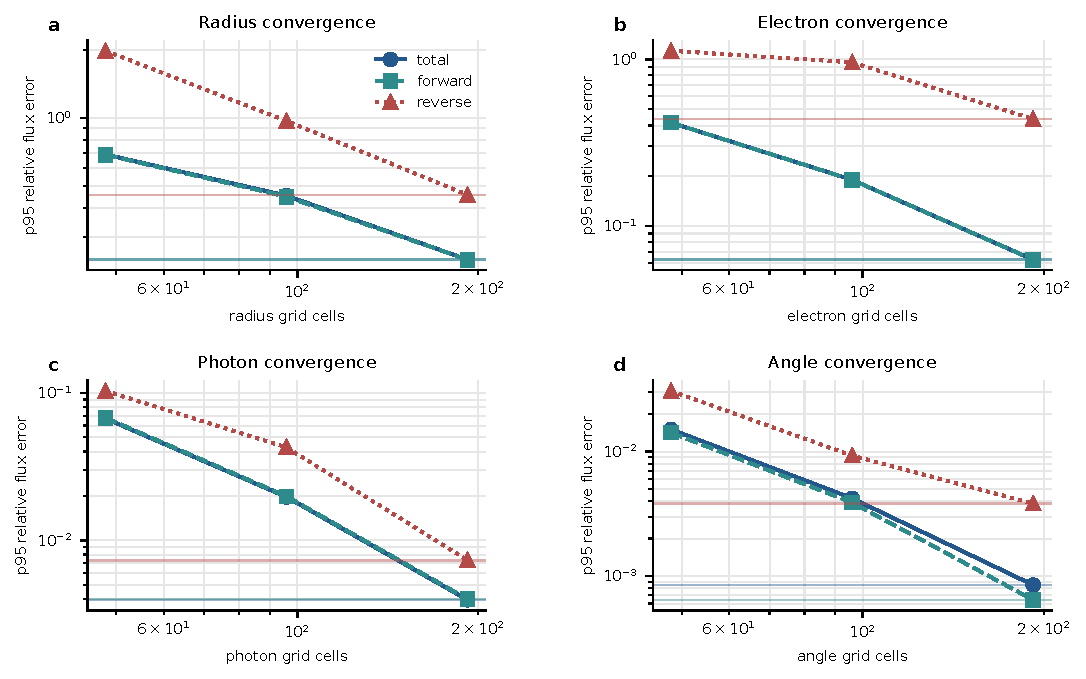
\includegraphics[width=\textwidth]{figures/fig5_validation_benchmark.pdf}
  \caption{
\gptareaderanchor{gpta-seg-000545}%
验证与可重复性仪表板。（a）表格介质与多跳介质的事件分裂动力学误差。（b）直接角度投影与声明的\(N_\theta^{\rm ref}\times N_\phi^{\rm ref}\)网格的对比。（c）反向冲击自适应网格相对于直接网格的差异。（d）一维和二维特征诊断的传输-重映射通量变化。这些图仅测试记录路径。}
  \label{fig:validation}
\end{figure*}

\clearpage
\onecolumngrid

\subsection{跨代码基准证据}


\gptareaderanchor{gpta-seg-000546}%
跨代码基准测试层仅测试声明了共同假设的公共输出子集。正式源表格为\texttt{paper/source\_data/}目录下的FigB1、FigB2和FigB3 CSV文件。FigB1是公共最小FS同步辐射案例。FigB2将ASGARD--\vegas\ RS/SSC子集与高斯离轴FS几何子集分开。FigB3是仅针对ASGARD的状态仪表板，用于强子、对反馈和\(\chi\)解析量。因此，FigB1和FigB2审核匹配的公共输出，而FigB3审核ASGARD内部的状态可见性。不支持的支路被标记为不支持，且不赋予误差值。

\begin{center}
\refstepcounter{table}\label{tab:cross-code-capabilities}
\small \textbf{表~\thetable.} 跨代码能力与基准证据映射。
\vspace{0.6ex}

\scriptsize
\setlength{\tabcolsep}{3pt}
\renewcommand{\arraystretch}{1.18}
\begin{tabular}{p{0.24\columnwidth}p{0.64\columnwidth}}
\hline
代码 & 能力与证据映射\\
\hline
ASGARD & 通道：FS 同步辐射、FS SSC/IC、可选 RS、壳层平均强子与电子对反馈、吸收、观测者组装。几何/介质：均匀介质、\(k=2\) 恒星风、表格化介质、结构化分量。状态：动力学、粒子、光子、分量和诊断。证据：图~\ref{fig:radius-state}--\ref{fig:validation}、图~\ref{fig:hadronic-feedback} 以及 FigB1--FigB3 源表。边界：无 \(\chi\) 分辨强子输运、无 IC 介导电磁级联、无喷流扩展后端、无自定义介质派发，且无 \(k\ne2\) 风介质。\\
\afterglowpy & 通道：FS 同步辐射。几何/介质：结构喷流和离轴观测者。状态：通量产物，而非 ASGARD 半径排序局部状态。证据：FigB1 FS 行和 FigB2 高斯几何行。边界：不用于 ASGARD RS、SSC、强子、电子对或局部状态主张。\\
\jetsimpy & 通道：FS 同步辐射。几何/介质：结构喷流和离轴观测者。状态：通量产物，而非 ASGARD 半径排序局部状态。证据：FigB1 FS 行和 FigB2 高斯几何行。边界：此处使用的公共分支不支持 ASGARD RS/SSC 或局部状态仪表板。\\
\vegas & 通道：包 API 暴露的公共余辉通道。几何/介质：包 API 暴露的公共几何和介质控制。状态：通量产物，而非 ASGARD 半径排序局部状态。证据：FigB1 FS 行，以及 FigB2 RS/SSC 和高斯几何行。边界：作为匹配接口比较使用，而不是 ASGARD 完整动力学目标。\\
PyBlast & 通道：公共余辉包接口。几何/介质：包 API 暴露的公共几何和介质控制。状态：包产物，而非 ASGARD 半径排序局部状态。证据：已安装源码提交、编译后的仓库本地 \texttt{pba.out}、FigB1 FS 行和 FigB2 高斯几何行。边界：不用于 ASGARD RS/SSC、强子、电子对或 \(\chi\) 分辨状态主张。\\
\hline
\end{tabular}
\end{center}

\begin{center}
\refstepcounter{figure}\label{fig:benchmark-fs}
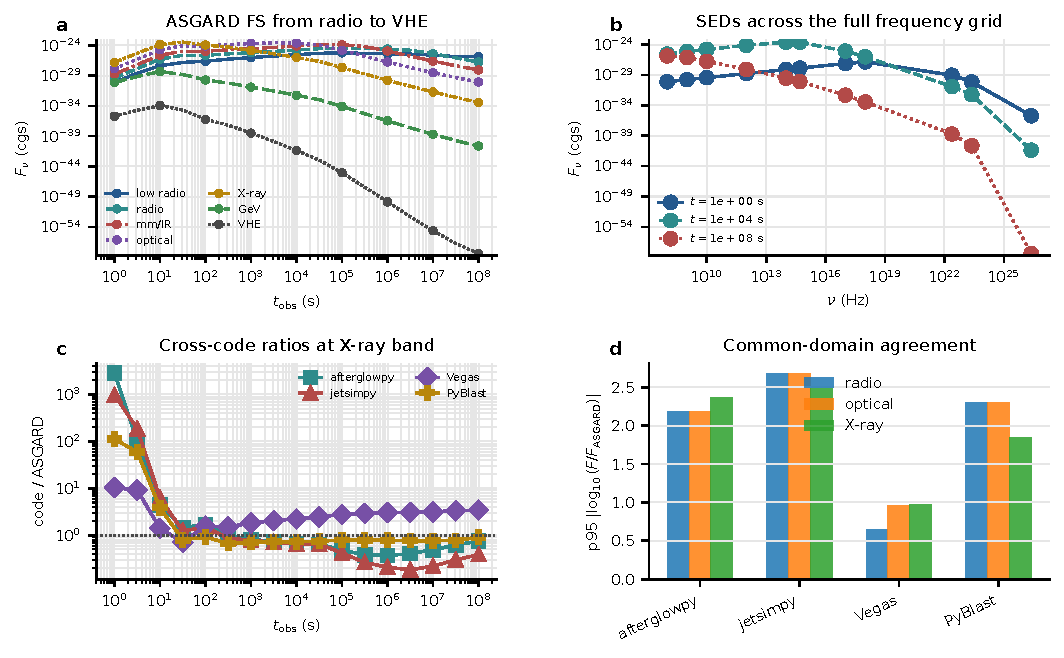
\includegraphics[width=0.94\textwidth]{figures/fig6_cross_code_fs_benchmark.pdf}

\small \textbf{图~\thefigure.} 前向激波共同最小基准。源表为 \texttt{paper/source\_data/figB1\_cross\_code\_fs.csv}。各行使用顶帽、轴上、均匀介质 FS 同步辐射设置，范围为 \(1\le t_{\rm obs}\le10^8\,{\rm s}\) 和 \(10^8\le\nu\le2.4\times10^{26}\,{\rm Hz}\)。(a) ASGARD 宽带光变曲线。(b) 早期、中期和晚期观测时刻的 ASGARD SED。(c) 具有数值行的公共工具在 X 射线波段的代码/ASGARD 比值。(d) 同一机器和同一场景下的墙钟时间。这些比值审核匹配假设；它们并不意味着所有包共享相同的吸收、截断或高能物理。
\end{center}

\begin{center}
\refstepcounter{figure}\label{fig:benchmark-rs-ssc-geometry}
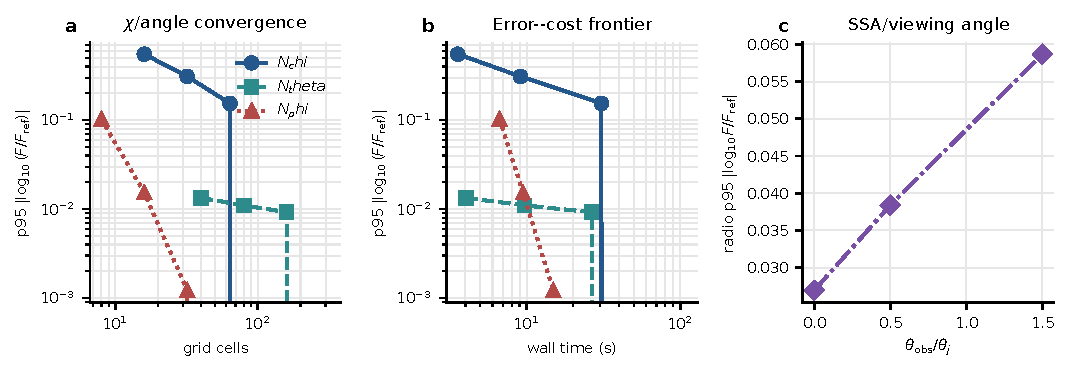
\includegraphics[width=0.94\textwidth]{figures/fig7_multiphysics_geometry_benchmark.pdf}

\small \textbf{图~\thefigure.} 匹配的多物理与几何基准子集。源表为 \texttt{paper/source\_data/figB2\_rs\_ssc\_geometry.csv}。RS/SSC 子集覆盖 ASGARD--\vegas\ 匹配顶帽设置中的 \(1\le t_{\rm obs}\le10^7\,{\rm s}\) 与 \(10^8\le\nu\le2.4\times10^{26}\,{\rm Hz}\)。(a) ASGARD 光学分量切片。(b) 宽网格上的 \vegas/ASGARD 分量比值中位数。高斯离轴 FS 子集覆盖 ASGARD、\afterglowpy、\jetsimpy 和 \vegas 的 \(10\le t_{\rm obs}\le10^8\,{\rm s}\) 与 \(10^8\le\nu\le2.4\times10^{23}\,{\rm Hz}\)。(c) 和 (d) 展示 ASGARD 多波段几何光变曲线和 X 射线几何比值。不支持通道是显式边界行，而不是失败的基准点。
\end{center}

\begin{center}
\refstepcounter{figure}\label{fig:benchmark-complex-state}
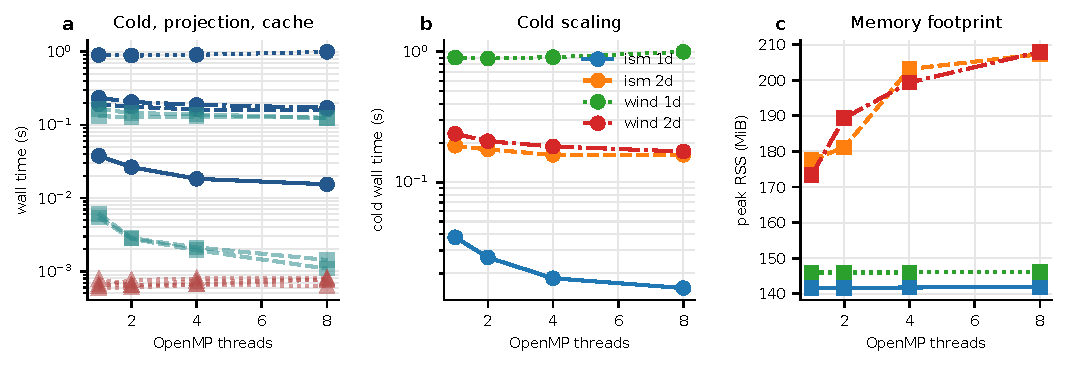
\includegraphics[width=0.94\textwidth]{figures/fig8_asgard_complex_state_dashboard.pdf}

\small \textbf{图~\thefigure.} ASGARD 复杂状态仪表板。源表为 \texttt{paper/source\_data/figB3\_asgard\_complex\_state.csv}。(a) 半径排序网格上的局部强子与电子对反馈状态能量。(b) 前向激波同步辐射投影分支的 \(\chi\) 分辨 SSA 状态。(c) \(\Gamma\)、\(B'\) 和电子能量的归一化链。该图测试 ASGARD 状态可见性和分量核算；它不是跨代码比值图。强子和电子对反馈行为一维且壳层平均；不支持 \(\chi\) 分辨强子反馈。
\end{center}


\gptareaderanchor{gpta-seg-000547}%
基准证据仅支持有界方法的主张。完成的图表展示了局部状态记录、组件核算、RS诊断、投影检查、匹配的公共输出子集以及仅限ASGARD的状态仪表板。表~\ref{tab:cross-code-capabilities}说明了哪些行具有数值证据，哪些行是边界。不受支持的开关组合并非模型预测。

\clearpage
\twocolumngrid

\section{讨论} \label{sec:discussion}

\subsection{简并性}


\gptareaderanchor{gpta-seg-000548}%
余辉光变曲线是简并的，因为多个局域过程可以改变相同的观测者流量。\(F_\nu(t_{\rm obs})\)中的转折可能追踪爆震波减速、密度结构、冷却转变、角度投影、RS成分、SSC冷却、局域吸收或次级粒子。ASGARD通过存储半径局域状态，在观测者投影混合角度和径向贡献之前，来解决这种简并性。图~\ref{fig:radius-state}至\ref{fig:reverse-shock}以及图~\ref{fig:benchmark-complex-state}展示了在解释光变曲线特征之前可以检查的局域记录。然后，图~\ref{fig:benchmark-fs}和\ref{fig:benchmark-rs-ssc-geometry}仅测试那些假设可以在代码间匹配的公开输出子集。这一证据支持诊断分解，而非声称某条光变曲线具有唯一的物理原因。

\subsection{状态}


\gptareaderanchor{gpta-seg-000549}%
半径有序状态是使基准测试可解释的对象。它将同一激波半径处的动力学、电子分布、光子场、吸收因子、可选的RS状态、可选的强子及对产物、以及观测者分量联系起来。状态图展示了ASGARD内部的这种联系，而跨代码图则显示了哪些投影输出可以与公共代码进行比较。这种区分很重要，因为公共通量比并不能揭示产生该通量的局部电子谱、光子场或对源。因此，图~\ref{fig:benchmark-complex-state} 补充了图~\ref{fig:benchmark-fs}--\ref{fig:benchmark-rs-ssc-geometry}：它在无法获得公平的公共代码比率时检查状态的完备性。

\subsection{边界}


\gptareaderanchor{gpta-seg-000550}%
受支持状态记录还定义了方法的停止位置。只有当ASGARD对某个分支具有局部状态、投影规则和验证证据时，该耦合物理分支才被视为受支持。表~\ref{tab:cross-code-capabilities}和章节~\ref{sec:limits}明确规定了这一规则，针对比较代码、运行时配置以及耦合物理分支。不支持的组合直接列为不支持，而非通过部分字段推断。因此，边界列表是方法的一部分，而非软件附注。

\section{模型边界} \label{sec:limits}

\subsection{运行时配置边界}


\gptareaderanchor{gpta-seg-000551}%
运行时配置边界状态决定了哪些输入具有完整的半径有序状态序列和观测器投影。设\(N_{\rho,\max}\)为列表介质容量，\(N_{J,\max}\)为密度跃变寄存器长度。凡不属于以下列表的设置均不被本文稿视为支持的物理模型。
\begin{itemize}
\item
\gptareaderanchor{gpta-seg-000552}%
外部介质支持均匀介质、\(k=2\)恒星风或表格化径向分布。不支持用户定义的介质内核。
\item
\gptareaderanchor{gpta-seg-000553}%
一个表格化的介质需要 \(2\le N_\rho\le N_{\rho,\max}\) 个正的半径-密度点，按半径递增排序。
\item
\gptareaderanchor{gpta-seg-000554}%
密度跃迁要求在解析介质上具有\(N_J\le N_{J,\max}\)个高斯跳跃。
\item
\gptareaderanchor{gpta-seg-000555}%
喷流扩散未得到支持。角度元素保持由初始喷流剖面指定的张角。
\item
\gptareaderanchor{gpta-seg-000556}%
自适应观察者时间网格仅支持直接顶帽核支持的模型。
\item
\gptareaderanchor{gpta-seg-000557}%
结构化的Fortran后端要求均匀的块采样，并且要么使用\texttt{fullhide\_1d}，要么使用\texttt{dg\_1d}。
\item
\gptareaderanchor{gpta-seg-000558}%
非均匀主导区域采样是一种补丁后端选项；结构化Fortran后端不支持它。
\item
\gptareaderanchor{gpta-seg-000559}%
目前的手稿证据集不支持天空图像和同步加速器-斯托克斯产品。
\item
\gptareaderanchor{gpta-seg-000560}%
热电子仅由一维隐式电子求解器支持。
\end{itemize}

\subsection{耦合物理边界}


\gptareaderanchor{gpta-seg-000561}%
耦合物理边界指出，额外辐射分支同时具备局域状态和观测者投影。缺少这两个要素的分支不用于模型预测。
\begin{itemize}
\item
\gptareaderanchor{gpta-seg-000562}%
正式强子输运需要一个一维前向电子求解器。
\item
\gptareaderanchor{gpta-seg-000563}%
遗留强子分支不支持 \(p\gamma\) 相互作用或中微子通道。
\item
\gptareaderanchor{gpta-seg-000564}%
联合电子-光子耦合需要一维隐式电子求解器、基于AM3的一维强子求解器、Hummer-2010光强子响应、Bethe-Heitler物理、数值IC/KN冷却、无反向激波、无\(\chi\)分辨输运以及固定电子子步长。
\item
\gptareaderanchor{gpta-seg-000565}%
多密度反向激波v1需要\(p_r>2\)。它不支持强子过程、前向SSC、反向SSC、跨区IC或联合电子-光子耦合。
\item
\gptareaderanchor{gpta-seg-000566}%
目前的正式强子路径是壳层平均的；它不是\(\chi\)分辨的。
\item
\gptareaderanchor{gpta-seg-000567}%
对级联迭代支持壳层序列 \(\gamma\gamma\) 对/同步反馈。逆康普顿散射介导的电磁级联不受支持。
\item
\gptareaderanchor{gpta-seg-000568}%
\(\chi\)分辨投影仅取代前向激波同步辐射和SSA投影。它不会使SSC、强子发射或对级联成为\(\chi\)局域。
\end{itemize}

\gptareaderanchor{gpta-seg-000569}%
这些限制是已发布方法的一部分。此列表之外的耦合情况没有手稿级别的支持，除非它有自己的本地状态、投影算子和验证证据。

\section{总结} \label{sec:summary}


\gptareaderanchor{gpta-seg-000570}%
\asgard\ 是一种有界 GRB 余辉方法，用于将观测者特征追溯至局部物理状态。在每个半径处，状态 \(\mathcal{S}(R)\) 记录了爆震波动力学、电子分布、光子场、可选强子种类、反向激波变量、吸收因子以及观测者分量。代码在应用等到达时间投影前更新这些对象。这一排序是本文的主要贡献：复杂的光变曲线可被解读为局部动力学、粒子、光子、吸收、分量和投影，而不仅仅是最终的 \(F_\nu(t_{\rm obs})\)。

该方法的证据可从跟踪的源数据中复现。图表测试了半径状态、正向激波 API 产物、电子与光子输运、\(\chi\) 分辨投影、反向激波诊断、强子/电子对激活检查、有界验证仪表盘、匹配的公共输出子集以及仅 ASGARD 状态仪表盘。能力表标明了哪些条目具有数值行，哪些条目是显式边界。PyBlastAfterglowMag 源已固定，其仓库本地的 \texttt{pba.out} 已编译，其数值行仅针对匹配的 FS 和高斯几何子集引用。

支持的使用案例恰好包含状态、投影和验证证据的案例。ASGARD 支持第~\ref{sec:limits} 节中列出的运行时和耦合物理领域。它不支持射流扩散、用户定义介质核、\(k\ne2\) 的风轮廓、\(\chi\) 分辨强子输运、IC 介质电磁级联，或没有经验证观测者投影的耦合分支。这些边界是方法的一部分，因为它们指明了从导出状态能够得出哪些物理解释。

\appendix

\gptareaderanchor{gpta-seg-000571}%
\setcounter{figure}{0}
\renewcommand{\thefigure}{A\arabic{figure}}
\renewcommand{\theHfigure}{A\arabic{figure}}

\section{电子求解器} \label{app:electron-solvers}


\gptareaderanchor{gpta-seg-000572}%
本附录记录了电子求解器的机制，这些机制对于主方法流程而言过于详细。正文保留了物理连续性方程、源项、冷却项、一个代表性更新、输出和边界。此处我们保留了坐标映射、求积规则、重映射、扫描系数以及分支特定的传输公式。本附录中的所有电子能量网格均使用自然对数参考坐标 \(x_g=\ln\gamma_e\)，除非局部定义了不同的存储坐标。

\subsection{初始谱求积与坐标映射}


\gptareaderanchor{gpta-seg-000573}%
在任何保守输运步骤之前，必须将初始电子谱转换为网格平均值。令 \(x_g=\ln\gamma_e\)，并令 \(N_x=dN_e/dx_g\) 为每个自然对数能量区间内的电子密度。对于 \(N_x\) 的任何连续段，固定的高斯--勒让德规则是
\begin{equation}
\int_a^b F(x)\,dx\simeq
\frac{b-a}{2}\sum_{q=1}^{N_{\rm G}} w_q^{\rm G}
F\!\left[\frac{a+b}{2}+\frac{b-a}{2}\xi_q\right],
\end{equation}

\gptareaderanchor{gpta-seg-000574}%
其中 \(F(x)\) 是被积分的区间，而 \((\xi_q,w_q^{\rm G})\) 是固定的节点和权重。如果求解器存储的是坐标 \(y\) 而非 \(x_g\)，则存储的是相同的物理谱，作为
\begin{equation}
N_{y,j}^{\rm init}=\frac{1}{\Delta y_j}
\int_{y_{j-1/2}}^{y_{j+1/2}}
N_x[x_g(y)]\,\frac{dx_g}{dy}\,dy .
\end{equation}

\gptareaderanchor{gpta-seg-000575}%
这个方程仅仅是变量的变化。它并不改变注入的电子能谱。

log-gamma分支直接存储自然对数能量坐标。在该分支中，
\begin{equation}
y=x_g,\qquad \gamma_e(y)=\exp(y),\qquad \frac{dx_g}{dy}=1.
\end{equation}

\gptareaderanchor{gpta-seg-000576}%
四速度分支存储一个不同的坐标，使得能谱的低能和高能部分可以在一个网格上表示。定义
\begin{equation}
\begin{gathered}
s\equiv\gamma_s^2-1,\\
\mathcal{Y}(\gamma)\equiv
\ln\left[1+\frac{\gamma^2-1}{s}\right].
\end{gathered}
\end{equation}

\gptareaderanchor{gpta-seg-000577}%
存储的坐标为 \(y=\mathcal{Y}(\gamma_e)\)。用于细胞平均转换的逆映射和雅可比矩阵为
\begin{equation}
\begin{aligned}
\gamma_e(y)&=\left[1+s(\exp(y)-1)\right]^{1/2},\\
x_g(y)&=\ln\gamma_e(y),\\
\frac{dx_g}{dy}&=\frac{s\exp(y)}{2\gamma_e^2}.
\end{aligned}
\end{equation}

\gptareaderanchor{gpta-seg-000578}%
这里，\(\gamma_s\) 设定了坐标从对数四速度行为转变为对数能量行为的位置。它是一个坐标参数，而非辐射截止点。

电子网格在存储坐标 \(y\) 上是均匀的。具有 \(N_\gamma\) 个网格单元的网格具有
\begin{equation}
\begin{aligned}
y_{i+1/2}&=y_L+\frac{i}{N_\gamma}(y_H-y_L),\\
y_L&=\mathcal{Y}(\gamma_{\min}),\qquad
y_H=\mathcal{Y}(\gamma_{\max}).
\end{aligned}
\end{equation}

\gptareaderanchor{gpta-seg-000579}%
返回给其余代码的诊断数组是
\begin{equation}
\begin{aligned}
x_{g,i+1/2}&=x_g(y_{i+1/2}),\\
\gamma_i&=\gamma_e\!\left[(y_{i-1/2}+y_{i+1/2})/2\right].
\end{aligned}
\end{equation}

\gptareaderanchor{gpta-seg-000580}%
条件 \(\gamma_s>1\) 和 \(\gamma_{\max}>\gamma_{\min}\) 给出了一个非零坐标区间。该设置的输出是一个保守存储网格以及恢复 \(dN_e/d\gamma_e\) 所需的雅可比矩阵。

\subsection{保守输运辅助器细节}


\gptareaderanchor{gpta-seg-000581}%
诊断需要 \(dN_e/d\gamma_e\)，即使求解器在 \(y\) 中存储了单元平均值。对于这种诊断转换，代码在每个单元内部重构一个正指数分布：
\begin{equation}
\frac{dN_e}{dy}=A_j\exp[\sigma_j(y-y_j)],
\qquad
y_j=\frac{y_{j-1/2}+y_{j+1/2}}{2}.
\end{equation}

\gptareaderanchor{gpta-seg-000582}%
对于具有正相邻平均值的内部单元，定义
\begin{equation}
\ell_j^-=\frac{\ln N_{y,j}-\ln N_{y,j-1}}{y_j-y_{j-1}},
\qquad
\ell_j^+=\frac{\ln N_{y,j+1}-\ln N_{y,j}}{y_{j+1}-y_j}.
\end{equation}
单调对数斜率为
\begin{equation}
\sigma_j=\operatorname{minmod}(\ell_j^-,\ell_j^+),
\end{equation}

\gptareaderanchor{gpta-seg-000583}%
而对于没有正相邻平均值的单元格，\(\sigma_j=0\)。
单元格平均值确定振幅：
\begin{equation}
A_j=
\begin{cases}
N_{y,j}, & z_j=0,\\
N_{y,j}\,z_j/\sinh z_j, & z_j\ne0,
\end{cases}
\qquad
z_j=\frac{1}{2}\sigma_j\Delta y_j .
\end{equation}

\gptareaderanchor{gpta-seg-000584}%
然后，居中的诊断电子密度为
\begin{equation}
\left.\frac{dN_e}{d\gamma_e}\right|_j
=
\frac{A_j}{d\gamma_e/dy}
=
\frac{A_j}{\gamma_j(dx_g/dy)_j}.
\end{equation}

\gptareaderanchor{gpta-seg-000585}%
此转换仅用于诊断目的。它允许一维、\(\chi\)分辨以及DG驱动程序导出壳层居中的\(dN_e/d\gamma_e\)记录，同时不改变传输的单元平均值。

冷却扫描将电子从高能迁移到低能，同时以守恒形式保持单元内容。令\(N_j\)为能量单元\(j\)中的电子数。面系数\(\lambda_{j+1/2}\)给出穿过单元\(j\)和\(j+1\)之间界面的数量通量，而\(b_0\)给出隐式步的对角权重。扫描系数为
\begin{equation}
\begin{aligned}
p_j&=b_0-\lambda_{j-1/2}\quad (j\ge2),\qquad p_1=p_2,\\
c_j&=\frac{2\lambda_{j+1/2}}{p_j+p_{j+1}} .
\end{aligned}
\end{equation}

\gptareaderanchor{gpta-seg-000586}%
从填充最多的箱开始，求解器评估
\begin{equation}
\begin{aligned}
N_N^{n+1}&=r_N,\\
N_j^{n+1}&=\Pi_+\!\left(r_j-c_jN_{j+1}^{n+1}\right).
\end{aligned}
\label{eq:triangular-cooling-sweep}
\end{equation}

\gptareaderanchor{gpta-seg-000587}%
此处\(r_j\)是源注入和对角线分割后的已知右侧项。\(\Pi_+\)将计算出的胞元内容投影到该守恒电子求解器所使用的非负域上。输出为冷却后的胞元平均谱\(N_j^{n+1}\)。

电子重映射在旧能量胞元和新能量胞元之间移动守恒的胞元内容。在本小节中，\(x\)表示自然对数坐标\(x_g=\ln\gamma_e\)。每次重映射都询问两个追踪胞元面之间有多少旧谱。对于点数据而言，局部二阶插值函数为
\begin{equation}
P_2(x)=\sum_{a=0}^{2}y_a\ell_a(x),
\qquad
\ell_a(x)=\prod_{b\ne a}\frac{x-x_b}{x_a-x_b}.
\end{equation}

\gptareaderanchor{gpta-seg-000588}%
这里\(y_a\)是三个相邻点的值，\(\ell_a\)是拉格朗日基函数。对于单元平均值，代码用抛物线轮廓重建每个单元内部的内容。在局部坐标\(\xi=(x-x_{j-1/2})/\Delta x_j\)中，
\begin{equation}
\begin{aligned}
Q_j(\xi)&=Q_{L,j}
+(Q_{R,j}-Q_{L,j}+Q_{6,j})\xi
-Q_{6,j}\xi^2,\\
Q_{6,j}&=6Q_j-3(Q_{L,j}+Q_{R,j}).
\end{aligned}
\end{equation}

\gptareaderanchor{gpta-seg-000589}%
此处\(Q_j\)是细胞平均值，\(Q_{L,j}\)和\(Q_{R,j}\)分别是左右界面值，而\(Q_{6,j}\)的选择使得细胞平均值恰好为\(Q_j\)。界面值被限制在相邻极值之间。局部极值使用\(Q_{L,j}=Q_{R,j}=Q_j\)。如果抛物线型剖面会在正值细胞内部引入负值内容，则界面偏差将按比例缩放。
\begin{equation}
\begin{aligned}
\theta_j&=\frac{Q_j}{Q_j-Q_{\min,j}},\\
Q_{L,R}&\leftarrow Q_j+\theta_j(Q_{L,R}-Q_j),
\end{aligned}
\end{equation}

\gptareaderanchor{gpta-seg-000590}%
其中 \(Q_{\min,j}\) 是单元内抛物线剖面的最小值。此操作保持单元平均值不变。对单元任意部分的积分是
\begin{equation}
\begin{aligned}
{\cal M}_j(\xi_l,\xi_r)
&=\Delta x_j\left[
Q_LD_1+\frac{Q_R-Q_L+Q_6}{2}D_2\right.\\
&\left.\hspace{3.0em}
-\frac{Q_6}{3}D_3
\right],
\end{aligned}
\end{equation}

\gptareaderanchor{gpta-seg-000591}%
其中 \(D_m\equiv\xi_r^m-\xi_l^m\)。前缀和给出 \(M(x)=\int_{x_{1/2}}^xQ(x')\,dx'\)。重映射利用 \(M(x)\) 精确移动位于两个追踪面之间的旧单元格内容。

解析源项与输运谱分开重建。这一点很重要，因为注入的幂律可以跨越 \(\gamma_e\) 的好几个数量级。如果三个相邻源单元格的平均值为正，则对数斜率是
\begin{equation}
\sigma_j=\operatorname{minmod}\left[
\frac{\ln Q_j-\ln Q_{j-1}}{x_j-x_{j-1}},
\frac{\ln Q_{j+1}-\ln Q_j}{x_{j+1}-x_j}
\right],
\end{equation}

\gptareaderanchor{gpta-seg-000592}%
且否则 \(\sigma_j=0\)。 利用此斜率，单元 \(j\) 中的重建源为
\begin{equation}
\begin{aligned}
Q_j(x)&=A_j\exp[\sigma_j(x-x_j)],\\
A_j&=Q_jG(z_j),\qquad z_j=\frac{\sigma_j\Delta x_j}{2},\\
G(z)&=
\begin{cases}
1, & z=0,\\
z/\sinh z, & z\ne0.
\end{cases}
\end{aligned}
\end{equation}

\gptareaderanchor{gpta-seg-000593}%
这里选择 \(A_j\) 使得单元平均值保持为 \(Q_j\)。该源剖面的积分是
\begin{equation}
{\cal S}_j(x_l,x_r)=
\begin{cases}
A_j\Delta x_{lr}, & \sigma_j=0,\\
A_j[E_j(x_r)-E_j(x_l)]/\sigma_j, & \sigma_j\ne0,
\end{cases}
\end{equation}

\gptareaderanchor{gpta-seg-000594}%
其中 \(\Delta x_{lr}\equiv x_r-x_l\) 且 \(E_j(x)\equiv\exp[\sigma_j(x-x_j)]\)。
为进行诊断，自然对数坐标内容被转换为以中心为基准的物理谱，通过
\begin{equation}
\left.\frac{dN_e}{d\gamma_e}\right|_j
=\frac{A_j}{\gamma_j},
\end{equation}

\gptareaderanchor{gpta-seg-000595}%
其中 \(x=\ln\gamma_e\)，\(\gamma_j=\exp(x_j)\)，而 \(A_j\) 是传输的 \(dN_e/dx\) 单元的重建幅度。

\subsection{特征与遗留重映射细节}


\gptareaderanchor{gpta-seg-000596}%
源耦合特征求积将源样本沿径向步放置。它使用 \(N_{\rm G}^{\rm C}\) 个高斯点和映射
\begin{equation}
s_m=t_m^{q_{\rm C}},\qquad
w_m=q_{\rm C}W_mt_m^{q_{\rm C}-1},
\end{equation}

\gptareaderanchor{gpta-seg-000597}%
其中 \(q_{\rm C}\) 是声明的源时聚类指数，\((t_m,W_m)\) 是区间 \([0,1]\) 上的高斯节点和权重。输出为径向区间内的一组源位置 \(s_m\) 和权重 \(w_m\)。

直接特征求解器追踪 \(u=1/\gamma_e\) 中的辐射冷却。利用 \(u_j=1/\gamma_{e,j}\)，它重构
\begin{equation}
w(u)=uD(u)
\end{equation}

\gptareaderanchor{gpta-seg-000598}%
在每个 \(u\) 细胞内，\(w(u)=A_u+S_u u\)。添加绝热冷却得到
\begin{equation}
\begin{aligned}
\frac{du}{dR}&=A_u+(S_u+b_{\rm ad})u,\\
b_{\rm ad}&=R_s^{-1}.
\end{aligned}
\end{equation}

\gptareaderanchor{gpta-seg-000599}%
解析反向映射应用于当前 \(u\) 单元内部。若追踪点到达单元边界，则使用新系数在相邻单元中计算剩余的径向滞后。结果即为每个到达面的出发位置。

随后，保守特征重映射使用两个前缀积分。设 \(M_N(x)\) 为传输谱 \(N_x\) 抛物重建的前缀积分，\(M_Q(x)\) 为源项重建 \(Q_x^{\rm C}\) 的前缀积分。对于到达单元 \(j\)，
\begin{equation}
\begin{aligned}
{\cal I}_N(j,\ell)&=
\frac{M_N[x_{j+1/2}^{\rm back}(\ell)]
-M_N[x_{j-1/2}^{\rm back}(\ell)]}{\Delta x_j},\\
{\cal I}_Q(j,\ell)&=
\frac{M_Q[x_{j+1/2}^{\rm back}(\ell)]
-M_Q[x_{j-1/2}^{\rm back}(\ell)]}{\Delta x_j}.
\end{aligned}
\end{equation}
更新后的单元平均值为
\begin{equation}
N_{x,j}^{n+1}={\cal I}_N(j,\Delta R)
+\Delta R\sum_{q=1}^{N_{\rm G}^{\rm C}}w_q{\cal I}_Q(j,s_q\Delta R).
\end{equation}

\gptareaderanchor{gpta-seg-000600}%
第一项沿着冷却特征携带旧电子。第二项在同一径向步长的正交位置添加源电子。

均匀网格半拉格朗日分支通过追踪单元格面来移动自然对数谱。它的源标签是 \(Q_{x,j}^{\rm S}\)。对于任何前缀积分 \(M\)，定义
\begin{equation}
\mathcal I_j(M;x_-,x_+)\equiv\frac{M(x_+)-M(x_-)}{\Delta x}.
\end{equation}

\gptareaderanchor{gpta-seg-000601}%
这里 \(x_-\) 和 \(x_+\) 是单元 \(j\) 的两个离开面，而 \(\mathcal I_j\) 返回它们之间的平均含量。该分支首先添加一半的源，然后回溯这些面：
\begin{equation}
\begin{aligned}
N_j^{1/2}&=\Pi_+\!\left(N_j^n+\frac{\Delta R}{2}Q_{x,j}^{\rm S}\right),\\
x_{j\pm1/2}^{\rm dep}
&=\Pi_x\!\left(x_{j\pm1/2}+\Delta R\,f_{j\pm1/2}\right),
\end{aligned}
\end{equation}

\gptareaderanchor{gpta-seg-000602}%
其中 \(f_{j\pm1/2}\) 是界面漂移，而 \(\Pi_x\) 将离开点保持在计算 \(x\) 域内。最终的单元平均值为
\begin{equation}
N_j^{n+1}
=\Pi_+\!\left[
\mathcal I_j(M_{1/2};x_{j-1/2}^{\rm dep},x_{j+1/2}^{\rm dep})
+\frac{\Delta R}{2}Q_{x,j}^{\rm S}
\right].
\end{equation}

\gptareaderanchor{gpta-seg-000603}%
该公式表明，旧电子从所追踪的出发区间积分而来，而源则被分割在冷却重映射的两侧。

三级自然对数求解器使用具有两组系数的三角冷却扫描。其源标签为 \(Q_{x,j}^{\rm 3}\)。在启动过程中，后向欧拉对角线、加载源的右侧项以及耦合系数
\begin{equation}
\begin{aligned}
p_j^{(1)}&=1-\lambda_{j-1/2}\quad (j\ge2),\qquad p_1^{(1)}=p_2^{(1)},\\
r_j^{(1)}&=\frac{N_j^n+\Delta R\,Q_{x,j}^{\rm 3}}{p_j^{(1)}},\\
c_j^{(1)}&=\frac{2\lambda_{j+1/2}}{p_j^{(1)}+p_{j+1}^{(1)}} .
\end{aligned}
\end{equation}

\gptareaderanchor{gpta-seg-000604}%
当两个历史状态可用时，分支使用二阶历史状态。系数为
\begin{equation}
\begin{aligned}
p_j^{(3/2)}&=\frac{3}{2}-\lambda_{j-1/2}\quad (j\ge2),\qquad
p_1^{(3/2)}=p_2^{(3/2)},\\
r_j^{(3/2)}&=
\frac{2N_j^n-\frac{1}{2}N_j^{n-1}+\Delta R\,Q_{x,j}^{\rm 3}}
{p_j^{(3/2)}},\\
c_j^{(3/2)}&=
\frac{2\lambda_{j+1/2}}{p_j^{(3/2)}+p_{j+1}^{(3/2)}} .
\end{aligned}
\end{equation}

\gptareaderanchor{gpta-seg-000605}%
这些系数输入到方程~\ref{eq:triangular-cooling-sweep}中的相同反向扫描。输出是守恒的自然对数单元平均谱。

WENO-Z自然对数分支从五单元模板重构显式面通量。其源标签为\(Q_{x,j}^{\rm W}\)。对于左偏界面，令\(f_m=F_{i+m}\)。三个候选通量为：
\begin{equation}
\begin{aligned}
\hat f_0&=\frac{1}{3}f_{-2}-\frac{7}{6}f_{-1}+\frac{11}{6}f_0,\\
\hat f_1&=-\frac{1}{6}f_{-1}+\frac{5}{6}f_0+\frac{1}{3}f_1,\\
\hat f_2&=\frac{1}{3}f_0+\frac{5}{6}f_1-\frac{1}{6}f_2 .
\end{aligned}
\end{equation}
Jiang--Shu 光滑性指标为
\begin{equation}
\begin{aligned}
\beta_0&=\frac{13}{12}(f_{-2}-2f_{-1}+f_0)^2
+\frac{1}{4}(f_{-2}-4f_{-1}+3f_0)^2,\\
\beta_1&=\frac{13}{12}(f_{-1}-2f_0+f_1)^2
+\frac{1}{4}(f_1-f_{-1})^2,\\
\beta_2&=\frac{13}{12}(f_0-2f_1+f_2)^2
+\frac{1}{4}(3f_0-4f_1+f_2)^2 .
\end{aligned}
\end{equation}

\gptareaderanchor{gpta-seg-000606}%
用于\(v_x>0\)的右偏通量是在\((f_{i-1},f_i,f_{i+1},f_{i+2},f_{i+3})\)上相同公式的镜像。两个能量端的常数虚拟单元提供了五点模板；它们是数值边界状态，不作为物理电子仓返回。

WENO径向更新在三个显式阶段中应用重建通量：
\begin{equation}
N_j^{(1)}=N_j^n+\lambda_W\mathcal{D}_j(N^n)+\Delta R\,Q_{x,j}^{\rm W},
\end{equation}
\begin{equation}
N_j^{(2)}=\frac{3}{4}N_j^n+
\frac{1}{4}\left[N_j^{(1)}+
\lambda_W\mathcal{D}_j(N^{(1)})\right]
+\frac{1}{4}\Delta R\,Q_{x,j}^{\rm W},
\end{equation}
\begin{equation}
N_j^{n+1}=\frac{1}{3}N_j^n+
\frac{2}{3}\left[N_j^{(2)}+
\lambda_W\mathcal{D}_j(N^{(2)})\right]
+\frac{2}{3}\Delta R\,Q_{x,j}^{\rm W}.
\end{equation}

\gptareaderanchor{gpta-seg-000607}%
这里 \(\lambda_W=\Delta R/\Delta x\) 且 \(\mathcal D_j=F_{j+1/2}-F_{j-1/2}\)。输出是对自然对数电子谱的显式有限差分更新，并在每个阶段添加源注入。

DG活动网格选择哪些电子能量元素需要多项式输运。它仅当旧谱仍携带足够的高能矩时才保留高能尾部。对于试验上限截断 \(\gamma_u\)，源支撑端点是
\begin{equation}
x_{\rm src}^{\max}=
\ln\left[\min(\gamma_{\max}^{\rm grid},\eta_{\rm tail}\gamma_u)\right],
\end{equation}

\gptareaderanchor{gpta-seg-000608}%
并且活跃的高能边缘被保持，当
\begin{equation}
\frac{\mathcal{M}_2(x_{\rm src}^{\max})}{\mathcal{M}_2^{\rm tot}}
>\epsilon_{\rm tail},
\qquad
\mathcal{M}_2^{\rm tot}\equiv\int N_y\gamma_e^2\,dy .
\end{equation}

\gptareaderanchor{gpta-seg-000609}%
这里 \(\mathcal M_2\) 是存储光谱的一个诊断高能矩。
它选择活动的DG区域；它不是一个物理电子截止。

密度跳跃径向子步进器在声明的密度结构附近选择较小的径向步长。它从
\begin{equation}
\Delta R_{\rm DG}=\frac{R_i-R_{i-1}}{N_{\rm DG}}.
\end{equation}

\gptareaderanchor{gpta-seg-000610}%
对于宽度为 \(\sigma_j=w_jR_j\) 的高斯密度跳跃，候选步长在标记的跳跃窗口处被截断。
\begin{equation}
R_j+\sigma_j\mathcal{Z}_{\rm J},
\end{equation}

\gptareaderanchor{gpta-seg-000611}%
在活动跳跃窗口内，该步骤遵循
\begin{equation}
\Delta R\le \frac{\sigma_j}{N_{\rm J}}.
\end{equation}

\gptareaderanchor{gpta-seg-000612}%
最后一步的边界使用了局部密度梯度尺度。
\begin{equation}
\begin{aligned}
g_n(R)&=1+\sum_j(f_j-1)
\exp\left[-\frac{(R-R_j)^2}{2\sigma_j^2}\right],\\
\Delta R&\le \frac{\eta_{\nabla n}}{|d\ln g_n/dR|}.
\end{aligned}
\end{equation}

\gptareaderanchor{gpta-seg-000613}%
这些界限控制了径向DG工作在快速外部密度变化附近的行为。

DG源模板归一化到同一\(y\)测度下的守恒有限单元源积分：
\begin{equation}
\widetilde Q_y^{\rm D}\leftarrow
\widetilde Q_y^{\rm D}
\frac{\sum_j \bar Q_{y,j}\Delta y_j}
{\int \widetilde Q_y^{\rm D}\,dy}.
\end{equation}


\gptareaderanchor{gpta-seg-000614}%
DG源投影将该源存储为每个活动单元内的勒让德矩。用\(P_m\)表示局部勒让德多项式，\(r(y)\)表示单元坐标，这些系数是
\begin{equation}
\begin{aligned}
\widehat Q_{am}&=
\frac{2m+1}{\Delta y_a}
\int_{y_{a,L}}^{y_{a,R}}Q_y(y)P_m[r(y)]\,dy,\\
Q_{a,i}&=\sum_{m=0}^{p_{\rm DG}}\widehat Q_{am}P_m(r_i).
\end{aligned}
\end{equation}

\gptareaderanchor{gpta-seg-000615}%
积分由高斯-勒让德求积法计算。反向激波动能源在同一坐标系中使用归一化形状：
\begin{equation}
\Phi_y^{\rm K}=A_{\rm K}\gamma_e
(\gamma_e-1)^{-p}\mathcal{C}_{\max}(\gamma_e)
\frac{dx_g}{dy}\,\mathbf{1}_{\gamma_e\ge\gamma_m},
\end{equation}

\gptareaderanchor{gpta-seg-000616}%
其中 \(A_{\rm K}\) 由所需的壳层积分动能源含量确定。

DG隐式输运块将多项式系数沿一个径向步长推进。它由Legendre--Gauss--Lobatto导数矩阵组装而成。对于元素 \(a\),
\begin{equation}
\begin{aligned}
A_{a,ij}&=\delta_{ij}
-\Delta R
\frac{2}{\Delta y_a}
\frac{w_j}{w_i}D_{ji}v_{y,j},\\
\sum_j A_{a,ij}N_{a,j}^{n+1}
&=N_{a,i}^{n}+\Delta R\,Q_{a,i}
+\mathcal{F}_{a,i}^{\rm up},
\end{aligned}
\end{equation}

\gptareaderanchor{gpta-seg-000617}%
其中\(D_{ji}=\left.dL_i/dr\right|_{r_j}\)，\(w_i\)为LGL求积权重，\(\mathcal{F}_{a,i}^{\rm up}\)为迎风边界贡献。该块是紧致主文本算子\(\mathcal A_a\)的局部形式。

DG守恒重映射将相同的电子洛伦兹因子从旧坐标传递到新坐标。节点密度映射为
\begin{equation}
N_{\rm n}(y_{\rm n})=
N_{\rm o}(y_{\rm o})
\frac{dy_{\rm o}}{dy_{\rm n}}
=
N_{\rm o}(y_{\rm o})
\frac{(dx_g/dy)_{\rm n}}{(dx_g/dy)_{\rm o}} .
\end{equation}

\gptareaderanchor{gpta-seg-000618}%
在投影或径向步之后，单元局部正性算子保持单元平均值。
\begin{equation}
\bar N_a=\frac{1}{2}\sum_iw_iN_{a,i}
\end{equation}
fixed and replaces nodal values by
\begin{equation}
\begin{aligned}
N_{a,i}&\leftarrow
\bar N_a+\theta_a(N_{a,i}-\bar N_a),\\
\theta_a&=\min\left[1,\frac{\bar N_a}{\bar N_a-N_{a,\min}}\right],
\end{aligned}
\end{equation}

\gptareaderanchor{gpta-seg-000619}%
当\(N_{a,\min}<0<\bar N_a\)时。最终一个数守恒因子与重新映射后的存储电子数\(N_{\rm tot}\)相匹配。这些操作作用于DG节点值；它们并不定义新的物理冷却过程。

DG特征投影仪使用解析仿射冷却映射。定义\(\eta_b=\exp(-b_{\rm ad}\Delta R)\)和\(\zeta_b=1-\eta_b\)。径向滞后\(\Delta R\)上的前向映射为
\begin{equation}
\gamma_e(R+\Delta R)=
\begin{cases}
\displaystyle \frac{\gamma_e(R)}
{1+a_{\rm rad}\gamma_e(R)\Delta R}, &
b_{\rm ad}=0,\\[1.1ex]
\displaystyle
\frac{\gamma_e(R)\eta_b}
{1+(a_{\rm rad}/b_{\rm ad})\gamma_e(R)
\zeta_b}, & {\rm otherwise},
\end{cases}
\end{equation}
到达能量 \(\gamma_{\rm now}\) 的逆映射为
\begin{equation}
\gamma_{\rm back}=
\begin{cases}
\displaystyle \frac{\gamma_{\rm now}}
{1-a_{\rm rad}\gamma_{\rm now}\Delta R}, &
b_{\rm ad}=0,\\[1.1ex]
\displaystyle \frac{\gamma_{\rm now}}
{\eta_b-(a_{\rm rad}/b_{\rm ad})\zeta_b\gamma_{\rm now}}, &
{\rm otherwise}.
\end{cases}
\end{equation}
随后，Gauss--Legendre 求积和 Legendre 模态矩将上游多项式投影到到达单元上。输出是在到达网格上冷却后电子谱的 DG 表示。

隐式通量分裂求解器把冷却写成穿过单元面的通量。给定面速度 \(v_{j+1/2}\)，保守更新为
\begin{equation}
\begin{aligned}
N_j^{n+1}&=N_j^n+\Delta RQ_j+F_{j+1/2}-F_{j-1/2},\\
F_{j+1/2}&=\frac{\Delta R}{\Delta x_j}
\left(v_{j+1/2}^{+}N_{j+1}^{n+1}
+v_{j+1/2}^{-}N_j^{n+1}\right).
\end{aligned}
\end{equation}
这里 \(F_{j+1/2}\) 是穿过单元 \(j\) 右面的通量。符号 \(v^+\) 和 \(v^-\) 为隐式步选择迎风单元，\(\Delta x_j\) 是局部单元宽度。预积分序列在将 \(\Delta R\,v_{j+1/2}\) 替换为面位移 \({\cal F}_{j+1/2}\)，并将 \(\Delta RQ_j\) 替换为源含量 \({\cal Q}_j\) 后使用同一个矩阵。

自然对数 \texttt{fullhide} 分支在固定网格上使用同一个从高能到低能的三角求解。其面速度和扫描系数为
\begin{equation}
\begin{aligned}
v_{j+1/2}&=D_{j+1/2}+\frac{1}{R},\\
\lambda_{j+1/2}&=-\frac{\Delta R}{\Delta x}v_{j+1/2},
\end{aligned}
\end{equation}
其中 \(D_{j+1/2}\) 是单元面处的辐射冷却系数，\(1/R\) 项是 \(x=\ln\gamma_e\) 中的绝热漂移。线性系统写作
\begin{equation}
\begin{aligned}
p_j&=1-\lambda_{j-1/2},\\
c_j&=\frac{2\lambda_{j+1/2}}{p_j+p_{j+1}},\\
r_j&=\frac{N_j^n+\Delta RQ_j}{p_j},
\end{aligned}
\end{equation}
并由方程~\eqref{eq:triangular-cooling-sweep} 中从高能到低能的扫描求解。空间--半径 \texttt{fullhide} 分支在一系列源列和耦合列上应用同一求解。对于子步 \(m\)，
\begin{equation}
(1+\lambda_{j-1/2}^{m})N_j^{m}
-\lambda_{j+1/2}^{m}N_{j+1}^{m}
=N_j^{m-1}+S_j^{m},
\end{equation}
其中 \(S_j^m\) 是该子步中加入的源项。最低能和最高能行使用各自唯一的相邻面。求解所有 \(m=1,\ldots,N_{\rm step}\) 列后，最后一列即为更新后的电子谱。

输运例程还为后续辐射调用返回诊断支撑范围。这些范围告诉辐射核哪些能量单元和 \(\chi\) 单元已被填充；它们不定义新的物理截断。若谱峰由三个为正的相邻单元采样，则通过 \((\ln\nu_{l,c,r},\ln P_{l,c,r})\) 上的对数抛物线估计：
\begin{equation}
\ln\nu_{\rm pk}
=x_c+\frac{(y_l-y_r)(x_c-x_l)}
{2(y_l-2y_c+y_r)},
\end{equation}
结果被限制在括定区间内。二维驱动器使用的活动能量范围和 \(\chi\) 范围为
\begin{equation}
\begin{aligned}
i_{\rm act}&=\max\left[i_{\rm lo},\,i_{\rm src},\,
\min(N_\gamma,i_{\rm pop}+1)\right],\\
Q_i&>\epsilon_\gamma Q_{\rm pk},\qquad
N_i>\epsilon_\gamma\max(N_{\rm pk},Q_{\rm pk}),\\
a_{\rm act}&=\min(N_\chi,a_{\rm pop}+1),\\
N_{\chi,a}&>\epsilon_\chi N_{\chi,\rm pk}.
\end{aligned}
\end{equation}
这里 \(i_{\rm lo}\) 是输运能量下限索引。量 \(Q_{\rm pk}\)、\(N_{\rm pk}\) 和 \(N_{\chi,\rm pk}\) 分别为源项峰值、能量布居峰值和 \(\chi\) 布居峰值。阈值 \(\epsilon_\gamma\) 和 \(\epsilon_\chi\) 将输运扫描限制在已填充单元中。径向子步估计使用最大的活动能量漂移，
\begin{equation}
\xi_{\max}=\max_{a\le a_{\rm act},\,i<i_{\rm act}}
\left|D_{ia}+A_{{\rm ad},a}\right|,
\end{equation}
其中 \(D_{ia}\) 是辐射漂移，\(A_{{\rm ad},a}\) 是绝热漂移。如果活动布居扫描没有发现活动漂移，例程会从存储网格报告子步大小，而不是从更小的活动子集报告。

\subsection{\texttt{fullhide\_1d} 固定子步细节}

\texttt{fullhide\_1d} 固定子步分支在一个径向壳层内分辨源注入和冷却。令 \(\Delta R_i=R_i-R_{i-1}\)，子步数和宽度为
\begin{equation}
\begin{aligned}
L_i&=\max\!\left[
N_{\rm fh,min},
\min\!\left(N_{\rm fh,max},
\left\lfloor\frac{\Delta R_i}{\Delta R_0}\right\rfloor\right)
\right],\\
\Delta R&=\frac{\Delta R_i}{L_i}.
\end{aligned}
\end{equation}
这里 \(N_{\rm fh,min}\) 和 \(N_{\rm fh,max}\) 是声明的算法控制量。每个子步具有径向宽度 \(\Delta R\)，该分支输出 \(R_i\) 处的电子谱。

在没有热电子分支的均匀介质中，固定子步可以累积为一次隐式求解。子步半径为
\begin{equation}
R_r=R_{i-1}+r\Delta R,\qquad r=1,\ldots,L_i .
\end{equation}
壳层上的总非热源归一化为
\begin{equation}
\mathcal{Q}_{i}
=a_{p,i}\sum_{r=1}^{L_i}\Delta R\,q_R(R_r,\Delta R),
\qquad a_{p,i}\equiv a_p(R_i).
\end{equation}
\(y\) 网格上的源形状为
\begin{equation}
\phi_y(R,y)\equiv
\gamma_e^{1-p}
\mathcal{C}_{\max}(\gamma_e)
\frac{dx_g}{dy}.
\end{equation}
这里 \(\mathcal{C}_{\max}\) 是高能截断因子。加入单元 \(j\) 的源含量为
\begin{equation}
\bar Q_{y,j}^{\rm int}
=\frac{\mathcal Q_i}{\Delta y_j}
\int_{y_{j-1/2}}^{y_{j+1/2}}\phi_y(R_i,y)\,dy ,
\end{equation}
穿过一个面的积分冷却位移为
\begin{equation}
\mathcal{F}_{j+1/2}=
\frac{\Delta R_i\bar D_{j+1/2}
+\sum_{r=1}^{L_i}\Delta R/R_r}
{(dx_g/dy)_{j+1/2}} .
\end{equation}
合并求解使用与单子步更新相同的三对角矩阵。它将 \(\Delta R\,v_{j+1/2}\) 替换为 \(\mathcal{F}_{j+1/2}\)，并将 \(\Delta R\,Q_j\) 替换为 \(\bar Q_{y,j}^{\rm int}\)，使壳层积分源和冷却位移进入同一次保守求解。

非均匀密度和热电子使用显式径向子步。在每个子步端点 \(R_r\)，求解器重新计算 \(n(R_r)\)、\(B'\)、\(\gamma_{\max}\) 和 \(\gamma_m\)。局部非热源为
\begin{equation}
Q_{y,j}^{(r)}
=\frac{q_R(R_r,\Delta R)a_p(R_r)}{\Delta y_j}
\int_{y_{j-1/2}}^{y_{j+1/2}}\phi_y(R_r,y)\,dy ,
\end{equation}
当 \texttt{thermal\_electrons} 启用时，还会加入 Maxwell--Juttner 源。辐射冷却系数先由壳层光子场组装一次，然后按局部密度缩放：
\begin{equation}
D_j(R_r)=D_j(R_{i-1})\frac{n(R_r)}{n(R_{i-1})}.
\end{equation}
当 \(\bar\Gamma_i\) 和壳层光子形状固定时，该缩放对局部同步辐射冷却是精确的。对于完整冷却数组，它是受支持的密度响应规则。

\subsection{耦合 \texttt{fullhide} 电子--光子系数}

耦合电子--光子通道使用与分离 \texttt{fullhide\_1d} 求解相同的三角原语。对于固定径向子步，对角系数和带源右端为
\begin{equation}
\begin{aligned}
p_j&=1-\lambda_{j-1/2}\quad (j\ge2),\qquad p_1=p_2,\\
r_j&=\frac{N_j^n+\Delta R\,Q_{x,j}}{p_j},
\end{aligned}
\end{equation}
其中 \(Q_{x,j}\) 包括自然对数网格上的主注入和次级电子对。相邻单元通过
\begin{equation}
c_j=\frac{2\lambda_{j+1/2}}{p_j+p_{j+1}} .
\end{equation}
这些系数进入方程~\eqref{eq:triangular-cooling-sweep} 中从高能到低能的扫描。它们只通过所提供的冷却场和次级源改变局部电子谱。

\subsection{混合热 \texttt{fullhide} 细节}

混合热分支由 \(\gamma_m\) 以下的热部分和 \(\gamma_m\) 以上的非热尾部构建一个注入源。它需要归一化积分，而不是新的输运方程。截断幂律尾部使用的上不完全 gamma 函数为
\begin{equation}
\Gamma(s,x)=\int_x^\infty t^{s-1}e^{-t}\,dt,
\end{equation}
Maxwell--Juttner 矩使用的修正 Bessel 函数为
\begin{equation}
\begin{aligned}
K_\nu(z)&=\int_0^\infty e^{-z\cosh u}\cosh(\nu u)\,du,\\
\nu&\in\{0,1\}.
\end{aligned}
\end{equation}
数值例程 \texttt{dgamic}、\texttt{dbsk0e} 和 \texttt{dbsk1e} 计算这些函数。它们提供截断幂律归一化
\begin{equation}
\int_{\gamma_m}^{\infty}\gamma^{-p}e^{-\gamma/\gamma_{\max}}\,d\gamma
=\gamma_{\max}^{1-p}
\Gamma\!\left(1-p,\frac{\gamma_m}{\gamma_{\max}}\right),
\end{equation}
以及热源中使用的 Maxwell--Juttner 矩。

热源只使用 \(\gamma_m\) 以下的 Maxwell--Juttner 含量。令 \(\gamma=\cosh u\)，
\begin{equation}
\sqrt{\gamma^2-1}\,d\gamma=\sinh^2u\,du .
\end{equation}
完整相对论矩为
\begin{equation}
\begin{aligned}
J_1(\Theta)&=2\Theta^2K_1(\Theta^{-1})
+\Theta K_0(\Theta^{-1}),\\
J_2(\Theta)&=(6\Theta^3+\Theta)K_1(\Theta^{-1})
+3\Theta^2K_0(\Theta^{-1}).
\end{aligned}
\end{equation}
这里 \(\Theta\) 是源归一化使用的无量纲热温度。代码减去 \(\gamma_m\) 以上的部分。令 \(a=\gamma_m/\Theta\)，尾部展开为
\begin{equation}
\begin{aligned}
\sqrt{\gamma^2-1}
&=\gamma\sum_{r=0}^{N_b} c_r\gamma^{-2r},\\
c_r&=(-1)^r\binom{1/2}{r},
\end{aligned}
\end{equation}
因此 \(b_r=-c_r\) 是扣除系数。\(\gamma_m\) 以下保留的矩为
\begin{equation}
\begin{aligned}
H_m(\Theta)&=\sum_{r=0}^{N_b}
b_r\Theta^{m+2-2r}\Gamma(m+2-2r,a),\\
I_1(\Theta)&=J_1(\Theta)+H_1(\Theta),\\
I_2(\Theta)&=J_2(\Theta)+H_2(\Theta).
\end{aligned}
\end{equation}
这里 \(N_b\) 是固定的热尾展开阶数。各项按递增的 \(r\) 累积；当下一项修正小于矩 \(I\) 的 \(\epsilon_{\rm th}\max(I,I_{\rm floor})\) 时，级数停止。对于非正阶数，递推式
\begin{equation}
\Gamma(s-1,a)=\frac{\Gamma(s,a)-a^{s-1}\exp(-a)}{s-1}
\end{equation}
从 \(\Gamma(0,a)\) 向下递推。这些控制量设定特殊函数计算；它们不定义电子分布中的物理截断。

热温度通过匹配请求的热含量确定。求解从 \(\Theta\) 上的对数网格开始：
\begin{equation}
\begin{aligned}
\Theta_r&=s_r\gamma_m,\\
s_r&=s_{\min}
\left(\frac{s_{\max}}{s_{\min}}\right)^{(r-1)/(N_s-1)},\\
r&=1,\ldots,N_s .
\end{aligned}
\end{equation}
量 \(s_{\min}\)、\(s_{\max}\) 和 \(N_s\) 是固定种子控制量。括定搜索按固定因子 \(q_{\rm br}\) 移动试探标度，直到下、上符号包围解。相邻变号条目之间的割线插值给出第一次迭代。温度是以下方程的根：
\begin{equation}
\begin{aligned}
F(\Theta)&=\frac{\gamma_m}{\Theta}+\ln I_1(\Theta)-\ln C,\\
\frac{dF}{d\Theta}
&=-\frac{\gamma_m}{\Theta^2}
+\frac{1}{I_1(\Theta)}\frac{dI_1}{d\Theta}
=-\frac{\gamma_m}{\Theta^2}+\frac{I_2(\Theta)}{\Theta^2I_1(\Theta)} .
\end{aligned}
\end{equation}
这里 \(C\) 是热部分请求的归一化常数。温度相对修正为
\begin{equation}
\frac{\Delta\Theta}{\Theta}
=\frac{F(\Theta)}
{\gamma_m/\Theta-\Theta^{-1}I_2(\Theta)/I_1(\Theta)} .
\end{equation}
迭代使用 \(\Theta\leftarrow\Theta-\Delta\Theta\)，并在 \(|\Delta\Theta/\Theta|<\epsilon_\Theta\) 时停止。如果在 \(N_\Theta\) 次更新内未满足该条件，则温度求解失败。

确定 \(\Theta\) 后，该分支计算混合注入密度。对数归一化为
\begin{equation}
\begin{aligned}
A_{\rm th}&=\ln(1-f_e)-\ln I_1,\\
A_{\rm pl}&=\ln f_e-\ln I_{\rm pl},
\end{aligned}
\end{equation}
其中 \(f_e\) 是非热份额，\(I_{\rm pl}\) 是非热尾部积分。密度为
\begin{equation}
\phi_{\rm h}(\gamma)=
\begin{cases}
\exp[L_{\rm th}(\gamma)],
&1<\gamma<\gamma_m,\\
\exp[L_{\rm pl}(\gamma)],
&\gamma\ge\gamma_m,\\
0,&\gamma\le1.
\end{cases}
\end{equation}
其中
\begin{equation}
\begin{aligned}
L_{\rm th}&=\ln[\gamma(\gamma^2-1)^{1/2}]
-\gamma/\Theta+A_{\rm th},\\
L_{\rm pl}&=-p\ln\gamma-\gamma/\gamma_{\max}+A_{\rm pl}.
\end{aligned}
\end{equation}
这里 \(L_{\rm th}\) 和 \(L_{\rm pl}\) 是热部分和非热部分的对数密度。若 \(L_{\rm th}\) 或 \(L_{\rm pl}\) 低于声明的指数截断 \(\ell_{\rm exp}\)，则该值位于被计算源支撑之外，并对单元积分贡献为零。该分支的输出是电子网格上的混合源轮廓 \(\phi_{\rm h}\)。

\subsection{\texorpdfstring{\(\chi\)}{chi} 分辨下游状态细节}

下游状态附录说明二维电子分支如何将壳层谱转换为前向激波后的局部单元。活动坐标是 \(q\)，而不是 \(\chi\)。激波前沿位于 \(q=0\)，活动下游区间终止于
\begin{equation}
\begin{aligned}
q_\ast&=1-\left(1-\frac{1}{r_{\rm sh}}\right)^{r_{\rm sh}},\\
\Delta q&=\frac{q_\ast}{N_\chi},\\
q_{a+1/2}&=a\Delta q,\qquad
q_a=\left(a-\frac{1}{2}\right)\Delta q .
\end{aligned}
\end{equation}
在第一个半径处，代码将单区谱放入第一个下游单元，
\begin{equation}
\begin{aligned}
U_{i1}(R_1)&=\frac{N_i^0}{\Delta q},\\
U_{ia}(R_1)&=0,\qquad a>1 .
\end{aligned}
\end{equation}
这里 \(N_i^0\) 是电子单元 \(i\) 中的初始壳层谱，\(U_{ia}\) 是 \(q\) 中的单元平均值。壳层谱由 \(\sum_a U_{ia}\Delta q\) 恢复。

下游几何为每个 \(q\) 单元给出半径和整体洛伦兹因子。对于外部密度剖面 \(n\propto R^{-k}\)，
\begin{equation}
\begin{aligned}
\bar q_a&=1-q_a,\\
\alpha_\chi&=\frac{4-k}{3-k},\\
\chi_{{\rm BM},a}&=\bar q_a^{-\alpha_\chi}.
\end{aligned}
\end{equation}
这里 \(k\) 是外部密度指数。给定激波前沿四速度 \(u_f=(\Gamma_f^2-1)^{1/2}\)、速度 \(\beta_f=u_f/\Gamma_f\) 和桥接权重 \(\omega_f=\beta_f^2\)，两个对数半径偏移为
\begin{equation}
\begin{aligned}
\lambda_{{\rm BM},a}&=-\frac{\chi_{{\rm BM},a}-1}
{4(4-k)\Gamma_f^2},\\
\lambda_{{\rm p},a}&=\frac{\ln \bar q_a}{r_{\rm sh}(3-k)} .
\end{aligned}
\end{equation}
第一个偏移是 Blandford--McKee 极限。第二个偏移是平面强激波极限。局部单元半径为
\begin{equation}
r_a=R\exp\!\left[\omega_f\lambda_{{\rm BM},a}
+(1-\omega_f)\lambda_{{\rm p},a}\right].
\end{equation}
该映射只为输运后的电子含量指定局部状态；它不添加新的动力学方程。

下游整体速度用同一个双极限桥接指定。极限四速度为
\begin{equation}
\begin{aligned}
u_{{\rm BM},a}&=\frac{u_f}{\chi_{{\rm BM},a}^{1/2}},\\
\beta_{{\rm p},a}&=\beta_f e^{\lambda_{{\rm p},a}},\\
u_{{\rm p},a}&=\frac{\beta_{{\rm p},a}}
{(1-\beta_{{\rm p},a}^2)^{1/2}} .
\end{aligned}
\end{equation}
局部下游四速度和洛伦兹因子为
\begin{equation}
\begin{aligned}
u_a&=\sinh\!\left[\omega_f\sinh^{-1}u_{{\rm BM},a}
+(1-\omega_f)\sinh^{-1}u_{{\rm p},a}\right],\\
\Gamma_a&=(1+u_a^2)^{1/2},\qquad
\beta_a=\frac{u_a}{\Gamma_a}.
\end{aligned}
\end{equation}
这些量与局部半径一同存储，并随后进入冷却、发射、吸收和投影。

磁年龄度量一个下游单元离开激波图样已有多长时间。激波图样四速度为
\begin{equation}
\begin{aligned}
u_{\rm s,BM}&=(2\Gamma_f^2-1)^{1/2},\\
u_{\rm s,p}&=\frac{r_{\rm sh}}{r_{\rm sh}-1}u_f,\\
\Psi_{\rm s}&=\omega_f\sinh^{-1}u_{\rm s,BM}
+(1-\omega_f)\sinh^{-1}u_{\rm s,p},\\
u_{\rm s}&=\sinh\Psi_{\rm s},\qquad
\beta_{\rm s}=\frac{u_{\rm s}}{(1+u_{\rm s}^2)^{1/2}} .
\end{aligned}
\end{equation}
相对激波速度、共动单元宽度、累积距离和年龄为
\begin{equation}
\begin{aligned}
\beta_{{\rm rel},a}&=\frac{\beta_{\rm s}-\beta_a}
{1-\beta_{\rm s}\beta_a},\\
\Delta x'_a&=\Gamma_a\Delta x_{{\rm lab},a},\\
x'_a&=\sum_{b=1}^a\Delta x'_b,\\
t'_a&=\frac{x'_a}{\beta_{{\rm rel},a}c}.
\end{aligned}
\end{equation}
这里 \(t'_a\) 是只由磁场衰减分支使用的共动年龄。

在单元年龄已知后计算局部磁场。当磁场衰减激活时，磁场能量份额为
\begin{equation}
\epsilon_{B,a}=\epsilon_{B,\min}
+(\epsilon_B-\epsilon_{B,\min})
\left(1+\frac{t'_a}{t_B}\right)^{\alpha_t},
\end{equation}
否则 \(\epsilon_{B,a}=\epsilon_B\)。局部共动能量密度和磁场为
\begin{equation}
\begin{aligned}
e'_a&=r_{\rm sh}\Gamma_f(\Gamma_f-1)n(R)m_p c^2,\\
B'_a&=(8\pi\epsilon_{B,a}e'_a)^{1/2}.
\end{aligned}
\end{equation}
导出的场 \(B'_a\) 是局部同步辐射、自吸收、冷却和扩散核使用的磁场。

下游扩散系数由同一个局部磁场计算。对于下游单元 \(a\) 中的电子单元 \(i\)，
\begin{equation}
\begin{aligned}
r_{{\rm L},ia}&=\frac{\gamma_i m_ec^2}{eB'_a},\\
\kappa_{ia}&=\frac{c\,r_{{\rm L},ia}}{3}.
\end{aligned}
\end{equation}
该 Bohm 系数只由 \(\chi\) 分辨输运分支使用。

\subsection{\texorpdfstring{\(\chi\)}{chi} 分辨光子历史细节}

光子历史分支构造从更早单元到达每个下游单元的种子光子场。共动激波时间沿半径网格累积：
\begin{equation}
\begin{aligned}
t'_1&=0,\\
t'_j&=t'_{j-1}+
\frac{R_j-R_{j-1}}
{\bar\beta_j\bar\Gamma_j c},\\
\bar\Gamma_j&=\frac{\Gamma_j+\Gamma_{j-1}}{2}.
\end{aligned}
\end{equation}
这里 \(j\) 标记目标半径，\(m\) 标记更早的源半径。对于源单元 \(s=(m,a)\) 和目标单元 \(t=(j,b)\)，只有当源位于激波后方更远处且光有足够时间到达目标时，才使用该源：
\begin{equation}
\begin{aligned}
x'_{m,a}&\ge x'_{j,b},\\
c(t'_j-t'_m)&\ge x'_{m,a}-x'_{j,b}.
\end{aligned}
\end{equation}
有限源份额为
\begin{equation}
\begin{aligned}
w_s&=\min\left(1,\frac{c\Delta t'_m}{\Delta x'_{m,a}}\right),\\
\Delta t'_m&=t'_m-t'_{m-1},
\end{aligned}
\end{equation}
其中第一个区间取 \(\Delta t'_1=t'_2-t'_1\)。这些条件定义哪些旧光子进入局部冷却和 SSC 种子场。

光子历史分支把每个被接受的源谱映射到目标共动系。相对速度和多普勒因子为
\begin{equation}
\begin{aligned}
\beta_{st}&=\frac{\beta_t-\beta_s}{1-\beta_t\beta_s},\\
\Gamma_{st}&=(1-\beta_{st}^2)^{-1/2},\\
{\cal D}_{st}&=\Gamma_{st}(1+\beta_{st}) .
\end{aligned}
\end{equation}
目标频率 \(\nu'\) 在 \(\nu'_s=\nu'/{\cal D}_{st}\) 处读取源场。在两个正的源单元 \(\nu'_l<\nu'_s<\nu'_{l+1}\) 之间，源光度或光子密度场 \(Q\) 通过以下公式插值：
\begin{equation}
Q_s(\nu'_s)=Q_{s,l}
\exp\!\left[
\frac{\ln\nu'_s-\ln\nu'_l}
{\ln\nu'_{l+1}-\ln\nu'_l}
\ln\!\left(\frac{Q_{s,l+1}}{Q_{s,l}}\right)
\right].
\end{equation}
映射后的光度按 \(w_s{\cal D}_{st}^3\) 加权，而映射后的光子密度按 \(w_s{\cal D}_{st}^2\) 加权。含有非正插值端点的源区间贡献为零。

路径衰减将被接受的光子贡献乘以有限单元传递权重。对于一个光深区段，
\begin{equation}
\mathcal W(\tau)=
\begin{cases}
1, & \tau\to0,\\
(1-e^{-\tau})/\tau, & \tau>0 .
\end{cases}
\end{equation}
对于下游单元 \(a\) 内长度为 \(\Delta x'\) 的部分共动路径，
\begin{equation}
\tau_{\nu',a}^{\rm seg}
=\tau_{\nu',a}^{\rm prop}
\frac{\Delta x'}{\Delta x'_a}.
\end{equation}
令 \(a_+\) 和 \(a_-\) 分别表示包含上游端点 \(x'_+\) 和下游端点 \(x'_-<x'_+\) 的单元。完整衰减因子为
\begin{equation}
\begin{aligned}
{\cal A}_{\nu'}(x'_+,x'_-)
&=\mathcal W(\tau_{\nu',a_+}^{\rm seg})
\mathcal W(\tau_{\nu',a_-}^{\rm seg})e^{S_{\nu'}},\\
S_{\nu'}
&=\sum_{a=a_-+1}^{a_+-1}
\ln\mathcal W(\tau_{\nu',a}^{\rm prop}) .
\end{aligned}
\end{equation}
降阶冷却网格上的传播光深为
\begin{equation}
\begin{aligned}
\tau_{\nu',a}^{\rm prop}
&=\tau_{\nu',a}^{\rm SSA}
+\tau_{\nu',a}^{\gamma\gamma},\\
\tau_{\nu',a}^{\gamma\gamma}
&=\Delta x'_a\int \sigma_{\gamma\gamma}(\nu',\tilde\nu')
n_{\tilde\nu',a}\,d\tilde\nu' .
\end{aligned}
\end{equation}
因此，存储的历史场在作为冷却或 SSC 靶场使用之前，已经包含 SSA 和局部对不透明度。

流式光锥更新每次将同一历史场推进一个径向步。它存储从半径 \(j-1\) 到半径 \(j\) 的 \(P_{\nu',b}^{\rm stream}\) 和 \(n_{\nu',b}^{\rm stream}\)，因此目标单元 \(b\) 只需要区间
\begin{equation}
[x'_{j,b},\,x'_{j,b}+c(t'_j-t'_{j-1})].
\end{equation}
来自前一壳层单元 \(a\) 的新发射在以下重叠区间内贡献：
\begin{equation}
\begin{aligned}
x'_{{\rm L},ab}
&=\max(x'_{a-1/2,j-1},x'_{j,b}),\\
x'_{{\rm R},ab}
&=\min(x'_{a+1/2,j-1},x'_{j,b}+c\Delta t'_j),\\
w_{a\to b}^{(j)}
&=\frac{[x'_{{\rm R},ab}-x'_{{\rm L},ab}]_+}
{\Delta x'_{a,j-1}} .
\end{aligned}
\end{equation}
这里 \([z]_+=\max(z,0)\)。流式更新将同一个 \({\cal D}_{st}\)、正场插值和路径衰减同时应用于携带的历史场和新发射的前一壳层场。

\subsection{下游 \texorpdfstring{\(q\)}{q} 空间平流--扩散细节}

下游 \(q\) 输运附录给出单元平均量 \(U_{ia}\) 的有限体积更新。\(q\) 中的输运速度为
\begin{equation}
A_q(q,R)=\frac{(3-k)(q_\ast-q)}{R},
\end{equation}
其中 \(k\) 是外部密度指数。隐式分支推进的局部守恒律为
\begin{equation}
\frac{\partial U_i}{\partial R}
+\frac{\partial(A_qU_i)}{\partial q}
=\frac{\partial}{\partial q}
\left({\cal K}_i\frac{\partial U_i}{\partial q}\right)
+Q_i^{(1)}(R)\delta_{a1}.
\end{equation}
这里 \(Q_i^{(1)}\) 是已经除以第一个 \(q\) 单元宽度的激波前沿源。在特征能量分支中，同一个第一单元源在能量特征更新期间应用，而 \(q\) 重映射本身移动已有电子含量。

特征 \(q\) 重映射沿 \(q\) 中的局部流移动单元面。在下游单元 \(a\) 内，面速度重建为
\begin{equation}
A_q(q)=\alpha_a+\zeta_a q .
\end{equation}
位于 \(q_f^{n+1}\) 的面在 \(\Delta R\) 上通过下式回溯：
\begin{equation}
q_f^n=
\begin{cases}
\left(q_f^{n+1}+\alpha_a/\zeta_a\right)e^{-\zeta_a\Delta R}
-\alpha_a/\zeta_a, & \zeta_a\ne0,\\
q_f^{n+1}-\alpha_a\Delta R, & \zeta_a=0 .
\end{cases}
\end{equation}
如果回溯面穿过单元边界，则在下一个下游单元中重新开始同一个解析步骤，直到径向步长耗尽。

保守重映射从重建的分段抛物线轮廓读取电子含量。对于输入轮廓 \(U_i(q)\)，定义前缀积分
\begin{equation}
M_i(q)=\int_0^q U_i(q')\,dq' .
\end{equation}
重映射后的单元平均值为
\begin{equation}
U_{ia}^{\rm adv}
=\frac{M_i(q_{a+1/2}^{n})-M_i(q_{a-1/2}^{n})}{\Delta q}.
\end{equation}
该操作改变电子位于激波后的空间位置，但不改变其能量。

扩散度量把物理下游距离中的 Bohm 扩散转换为 \(q\) 网格上的扩散。使用桥接半径律，
\begin{equation}
\begin{aligned}
s(q)&=R-r(q),\\
J_q(q)&\equiv\frac{\partial q}{\partial s}
=\left[-R\frac{\partial(r/R)}{\partial q}\right]^{-1}.
\end{aligned}
\end{equation}
扩散面系数为
\begin{equation}
{\cal K}_{i,a+1/2}
=\frac{\kappa_{i,a+1/2}}{\beta_{\rm sh}c}
J_{q,a+1/2}^{2},
\end{equation}
面通量为
\begin{equation}
{\cal G}_{i,a+1/2}
={\cal K}_{i,a+1/2}
\frac{U_{i,a+1}-U_{ia}}{\Delta q}.
\end{equation}
这里 \(\kappa_{i,a+1/2}\) 是面平均 Bohm 系数，\(\beta_{\rm sh}\) 是激波速度。

隐式扩散求解使用中心面差分。对于右端状态 \(U_{ia}^{\rm rhs}\)，
\begin{equation}
\begin{aligned}
\delta_{a+}U_i^{n+1}
&=U_{i,a+1}^{n+1}-U_{ia}^{n+1},\\
{\cal G}_{a+}^{n+1}
&={\cal K}_{i,a+1/2}
\frac{\delta_{a+}U_i^{n+1}}{\Delta q},\\
\Delta_a{\cal G}^{n+1}
&={\cal G}_{a+}^{n+1}-{\cal G}_{a-}^{n+1},\\
U_{ia}^{n+1}
-\frac{\Delta R}{\Delta q}\Delta_a{\cal G}^{n+1}
&=U_{ia}^{\rm rhs}.
\end{aligned}
\end{equation}
联合隐式驱动器在加入来自 \(A_q\) 的迎风平流系数后，求解同一个三对角系统。如果可选吸收外边界激活，最后一个单元使用 \(U_{i,N_\chi+1}=0\)，因此最终对角项接收
\begin{equation}
{\cal K}_{i,N_\chi+1/2}U_{i,N_\chi}^{n+1}.
\end{equation}
否则外部扩散通量封闭。三对角求解后，已求解的单元平均值被投影为非负值。

\subsection{下游能量空间更新细节}

下游能量更新在自然对数电子网格 \(x=\ln\gamma_e\) 上冷却每个 \(q\) 列。在默认 log-gamma 分支中，局部冷却速度为
\begin{equation}
\xi_{i+1/2,a}=D_{i+1/2,a}+\frac{1}{R},
\end{equation}
其中 \(D_{i+1/2,a}\) 是辐射冷却系数，\(1/R\) 是壳层绝热项。令 \(\lambda_{i+1/2,a}=-(\Delta R/\Delta x)\xi_{i+1/2,a}\)，隐式反向扫描系数为
\begin{equation}
\begin{aligned}
H_{ia}&=1-\lambda_{i-1/2,a},\\
C_{ia}&=\frac{2\lambda_{i+1/2,a}}{H_{ia}+H_{i+1,a}},\\
\rho_{ia}&=\frac{U_{ia}^{n}}{H_{ia}} .
\end{aligned}
\end{equation}
解从高电子能量到低电子能量恢复：
\begin{equation}
\begin{aligned}
U_{N_\gamma,a}^{n+1}&=\rho_{N_\gamma,a},\\
U_{ia}^{n+1}
&=\Pi_+\!\left(\rho_{ia}-C_{ia}U_{i+1,a}^{n+1}\right).
\end{aligned}
\end{equation}
投影 \(\Pi_+\) 只作用于已求解的单元平均量，不混合相邻能量单元。输出是传递给辐射核的冷却后列 \(U_{ia}^{n+1}\)。

PWN/CR 输运选项使用局部下游绝热项，而不是全局 \(1/R\) 壳层项。在该分支中
\begin{equation}
\xi_{i+1/2,a}=D_{i+1/2,a}+A_{{\rm ad},a},
\end{equation}
其中
\begin{equation}
A_{{\rm ad},a}=
\frac{1}{3\beta_f}
\left(
\frac{2\beta_a}{r_a}
+\left.\frac{\partial\beta}{\partial r}\right|_a
\right).
\end{equation}
这里 \(r_a\) 和 \(\beta_a\) 来自下游几何。随后同一个反向扫描更新每个列，因此该选项只改变绝热系数，而不改变能量网格求解。

随机能量扩散选项在 \(x=\ln\gamma_e\) 中加入保守扩散步。令
\begin{equation}
\lambda_x=\frac{\Delta R\,\alpha_{\rm st}}{R\,\Delta x^2},
\end{equation}
内部方程为
\begin{equation}
\begin{aligned}
{\cal L}_{ia}^{n+1}
&=-U_{i-1,a}^{n+1}+2U_{ia}^{n+1}-U_{i+1,a}^{n+1},\\
U_{ia}^{n+1}+\lambda_x{\cal L}_{ia}^{n+1}
&=U_{ia}^{n}.
\end{aligned}
\end{equation}
低能和高能边界对角项为 \(1+\lambda_x\)，因此穿过两个网格边界的随机能量通量为零。

\section{光子、SSC 与 SSA 核} \label{app:photon-kernels}

本附录给出支撑主体粒子--辐射输运章节的技术性辐射核。物理对象包括局部同步辐射光度、种子光子密度、SSC 光度、自吸收加热系数以及光子生存因子。正文说明这些对象如何进入冷却、发射和观测者投影；本附录给出计算它们所用的求积、插值和核公式。

\subsection{辐射 ABI 绑定}

辐射 ABI 层将公共辐射产物映射到编译核。首次访问时，它绑定 \texttt{annihilation}、\texttt{cal\_ebl}、\texttt{ssc\_spec} 和 \texttt{ssc\_spec\_nonuniform}。这些名称只标识运行时入口点。除正文定义的 SSC 光度、局部对吸收和外部 EBL 衰减外，它们不添加新的光子状态。

Fan 式解析 Klein--Nishina 闭合估计有多少同步光子能量能够在 Thomson 区域散射。对于电子节点 \(i\)，阈值是其同步光子达到该节点 Klein--Nishina 极限的电子洛伦兹因子 \(\hat\gamma_i\)。电子上截断为 \(\gamma_M=\gamma_{\max}\)。以下公式输出 \(\eta_i^{\rm KN}\)，即阈值以下的光子能量份额。

在快冷却情形 \(\gamma_m>\gamma_c\) 中，相关谱从 \(\gamma_c\) 开始。定义
\begin{equation}
\begin{aligned}
A_f&=\frac{(p-1)\gamma_m}{p-2}-\gamma_c,\\
B_f&=\gamma_m^{p-1}\gamma_M^{2-p}
-(p-1)\gamma_m-(2-p)\gamma_c,\\
C_f&=(p-1)\gamma_m-(p-2)\gamma_c,\\
H_f(\hat\gamma_i)&=
\gamma_m^{p-1}(\gamma_M^{2-p}-\hat\gamma_i^{2-p}).
\end{aligned}
\end{equation}
\(\hat\gamma_i\) 以下的份额为
\begin{equation}
\eta_i^{\rm KN}=
\begin{cases}
0, & \hat\gamma_i<\gamma_c,\\[0.6ex]
\dfrac{\hat\gamma_i-\gamma_c}{A_f},
& \gamma_c\le\hat\gamma_i<\gamma_m,\ p>2,\\[2ex]
\dfrac{(2-p)(\hat\gamma_i-\gamma_c)}{B_f},
& \gamma_c\le\hat\gamma_i<\gamma_m,\ p\le2,\\[2ex]
1-\dfrac{\gamma_m^{p-1}\hat\gamma_i^{2-p}}{C_f},
& \gamma_m\le\hat\gamma_i<\gamma_M,\ p>2,\\[2ex]
1-\dfrac{B_f}{H_f(\hat\gamma_i)},
& \gamma_m\le\hat\gamma_i<\gamma_M,\ p\le2,\\[2ex]
1, & \hat\gamma_i\ge\gamma_M.
\end{cases}
\end{equation}
因此，当阈值低于最低快冷却断裂时，该分支返回零；当阈值高于截断时，返回一。

在慢冷却情形 \(\gamma_m\le\gamma_c\) 中，相关谱从 \(\gamma_m\) 开始。定义
\begin{equation}
\begin{aligned}
A_s&=\frac{\gamma_c^{3-p}}{p-2}-\gamma_m^{3-p},\\
B_s&=(3-p)\gamma_c\gamma_M^{2-p}
-\gamma_c^{3-p}-(2-p)\gamma_m^{3-p},\\
C_s&=\gamma_c^{3-p}-(p-2)\gamma_m^{3-p},\\
U_i&=\hat\gamma_i^{3-p}-\gamma_m^{3-p},\\
V_i&=(3-p)\gamma_c\hat\gamma_i^{2-p},\\
W_i&=(3-p)\gamma_c(\gamma_M^{2-p}-\hat\gamma_i^{2-p}).
\end{aligned}
\end{equation}
慢冷却份额为
\begin{equation}
\eta_i^{\rm KN}=
\begin{cases}
0, & \hat\gamma_i<\gamma_m,\\[0.6ex]
\dfrac{U_i}{A_s},
& \gamma_m\le\hat\gamma_i<\gamma_c,\ p>2,\\[2ex]
\dfrac{(2-p)U_i}{B_s},
& \gamma_m\le\hat\gamma_i<\gamma_c,\ p\le2,\\[2ex]
1-\dfrac{V_i}{C_s},
& \gamma_c\le\hat\gamma_i<\gamma_M,\ p>2,\\[2ex]
1-\dfrac{W_i}{B_s},
& \gamma_c\le\hat\gamma_i<\gamma_M,\ p\le2,\\[2ex]
1, & \hat\gamma_i\ge\gamma_M.
\end{cases}
\end{equation}
该分段值进入正文关系 \(Y_i^{\rm F}(1+Y_i^{\rm F})=\eta_{\rm rad}\eta_i^{\rm KN}\epsilon_e/\epsilon_B\)。该分支是逆康普顿冷却的解析闭合；它不替代完整 IC/KN 路径使用的表格化光子场。

SSA 加热求积计算与正文相同的被吸收光子能量积分。对于每个电子节点 \(i\)，代码首先找到包含 \(\nu_{\min,i}\) 和 \(\nu_{u,i}\) 的光子单元。它将这两个单元截断到物理积分区间，并用缓存的对数 Gauss 权重处理它们之间的所有完整单元。对于低频完整单元 \(\ell\)，令 \(\nu_{\ell q}\) 和 \(w_{\ell q}\) 为 \(x=\ln\nu\) 中的 \(N_{\rm G}\) 点节点和权重，并包含雅可比 \(d\nu=\nu\,dx\)。缓存的低频前缀为
\begin{equation}
\mathcal P_k
=hc\sum_{\ell=1}^{k}\sum_{q=1}^{N_{\rm G}}
w_{\ell q}n_\nu(\nu_{\ell q})\nu_{\ell q}^{-2/3}.
\end{equation}
如果完整低频单元从 \(k_1\) 延伸到 \(k_2\)，它们对加热系数的贡献为
\begin{equation}
A_{i,L}^{\rm abs}
=\kappa_1\frac{B_Q}{B'}(\chi_{\rm L}\nu_{\min,i})^{5/3}
\left(\mathcal P_{k_2}-\mathcal P_{k_1-1}\right).
\end{equation}
高频完整单元使用同一单粒子拟合的指数部分：
\begin{equation}
A_{i,H}^{\rm abs}
=\kappa_2\frac{B_Q}{B'}\gamma_i^{-3}\nu_B hc
\sum_{\ell,q} w_{\ell q}n_\nu(\nu_{\ell q})
\exp(-\nu_{\ell q}/\nu_{u,i}).
\end{equation}
被截断边界单元积分在截断频率范围上使用同样的两个分支。返回值为 \(A_i^{\rm abs}=A_{i,L}^{\rm abs}+A_{i,H}^{\rm abs}\) 加上两个截断单元项。共享插值原语在每个单元内提供 \(n_\nu\)；正端点使用 log--log 插值，非正端点使用线性分支。

网格级逆康普顿冷却路径在同一个局部频率网格上对种子光子和散射光子积分。如果存储的网格边界为 \(\nu_j\)，单元中心测度为
\begin{equation}
\begin{aligned}
\bar\nu_j&=(\nu_j\nu_{j+1})^{1/2},\\
\Delta\nu_j&=\bar\nu_j\left(\ln\nu_{j+1}-\ln\nu_j\right),\\
\epsilon_j&=\frac{h\bar\nu_j}{m_e c^2}.
\end{aligned}
\end{equation}
共享幂律插值给出 \(n_{\nu,j}=n_\nu(\bar\nu_j)\)。对于电子节点 \(i\)、种子单元 \(j\) 和散射单元 \(\ell\)，定义
\[
b_{ij}=4\gamma_i\epsilon_j,\qquad
q_{i\ell j}=\frac{\epsilon_\ell}{b_{ij}(\gamma_i-\epsilon_\ell)} .
\]

\gptareaderanchor{gpta-seg-000620}%
冷却积分中使用的分支核是
\begin{equation}
G_{i\ell j}=
\begin{cases}
\bar\nu_\ell/\bar\nu_j-(4\gamma_i^2)^{-1},
& \bar\nu_j/(4\gamma_i^2)<\bar\nu_\ell\le\bar\nu_j,\\[1ex]
G_{\rm J}(q_{i\ell j},b_{ij}),
& 0<q_{i\ell j}<1,\quad \epsilon_\ell<\gamma_i,\quad
  \epsilon_\ell\le\epsilon_{\max,ij},\\[1ex]
0, & {\rm otherwise},
\end{cases}
\end{equation}
其中 \(\epsilon_{\max,ij}=4\gamma_i^2\epsilon_j/(1+b_{ij})\)。冷却系数累积为
\begin{equation}
A_i^{\rm IC}\simeq
\frac{3h\sigma_{\rm es}}{4m_e c\gamma_i^3}
\sum_j\frac{n_{\nu,j}}{\bar\nu_j}\Delta\nu_j
\sum_\ell \bar\nu_\ell G_{i\ell j}\Delta\nu_\ell .
\end{equation}
这是正文 IC 损失积分的离散形式。

耦合预算逆康普顿路径使用同一个物理核，但改变隐式联合求解所用的求积权重。令 \(x_\nu=\ln\nu\)、均匀间距为 \(\Delta x_\nu\)、Simpson 权重为 \(w_j^{\rm S}\)，它返回
\begin{equation}
\begin{aligned}
A_i^{\rm IC,b}&=
\frac{3h\sigma_{\rm es}}{4m_e c\gamma_i^3}
\left(\frac{\Delta x_\nu}{3}\right)^2\\
&\quad\times
\sum_\ell w_\ell^{\rm S}\nu_\ell^2
\left[\sum_j w_j^{\rm S}n_{\nu,j}K_{i\ell j}\right].
\end{aligned}
\end{equation}
对于低于散射单元的种子单元，\(K_{i\ell j}=G_{\rm J}(q_{i\ell j},b_{ij})\)。对于等于或高于散射单元的种子单元，
\[
K_{i\ell j}=
\max\left[\frac{\nu_\ell}{\nu_j}-\frac{1}{4\gamma_i^2},0\right].
\]

\gptareaderanchor{gpta-seg-000621}%
输出的 \(A_i^{\rm IC,b}\) 是电子-光子联合求解的能量预算系数；它并不定义独立的 IC 冷却法则。

快速同步辐射发射率路径使用单粒子同步辐射核的解析近似。对于具有 \(\nu_c=C_\nu B'\gamma_e^2\) 的电子，定义 \(x=\nu/\nu_c\)。辐射回路所使用的核是
\begin{equation}
\Phi(x)=
\begin{cases}
A_\Phi x^{1/3}, & x<x_{\rm L},\\[1ex]
A_\Phi e^{-x}\left(x^{-2/3}+B_\Phi^2\right)^{-1/2},
& x_{\rm L}\le x\le x_{\rm H},\\[1ex]
0, & x>x_{\rm H}.
\end{cases}
\end{equation}
低 \(x\) 分支保留同步辐射渐近形式，中间分支承载高频指数下降，最后一个分支截断有限核表。常数 \(A_\Phi\)、\(B_\Phi\)、\(x_{\rm L}\) 和 \(x_{\rm H}\) 是该单粒子近似的固定系数；它们不是物理模型参数。

共享辐射插值原语在一个频率单元内计算表格化辐射场。对于相邻节点 \((\nu_0,Y_0)\) 和 \((\nu_1,Y_1)\)，正端点值使用局部幂律区段
\begin{equation}
\begin{aligned}
s_Y&=\frac{\ln(Y_1/Y_0)}{\ln(\nu_1/\nu_0)},\\
Y(\nu)&=Y_0\left(\frac{\nu}{\nu_0}\right)^{s_Y}.
\end{aligned}
\end{equation}
这里 \(Y\) 可以是同步辐射光度、吸收后光度、光深或光子密度。如果任一端点非正，辅助器使用两个存储值之间的线性区段。该规则只计算存储场；它不改变电子谱或光子状态。

对数 Gauss 辅助器在一个正频率单元上积分辐射场。令 \(x=\ln\nu\)、\(x_m=(\ln\nu_0+\ln\nu_1)/2\)、\(\Delta x=(\ln\nu_1-\ln\nu_0)/2\)，固定 \(N_{\rm G}\) 点规则使用
\begin{equation}
\begin{aligned}
\nu_a&=\exp(x_m+\Delta x\,\xi_a),\\
w_a&=\Delta x\,\omega_a\,\nu_a,\\
\int_{\nu_0}^{\nu_1}Y(\nu)\,d\nu
&\simeq \sum_{a=1}^{N_{\rm G}} w_a\,Y(\nu_a).
\end{aligned}
\end{equation}
这里 \(\xi_a\) 和 \(\omega_a\) 是 \([-1,1]\) 上的 Gauss--Legendre 节点和权重。\(w_a\) 中的因子 \(\nu_a\) 是 \(d\nu=\nu\,dx\) 的雅可比。降阶冷却表使用同一正频率坐标；对于至少 \(N_{\rm red}\) 个支撑点，它将最后一个点放在 \(\nu_{\max}\)，并把之前的点放在 \(\nu_{\min}\) 与由 \(f_{\rm tail}\) 设定的命名尾部位置之间。

SSA 加热区段返回一个频率区间内被吸收的光子能量。它使用与光子场辅助器相同的插值 \(n_\nu(\nu)\) 和相同的对数 Gauss 节点。对于具有局部系数 \(\Sigma_{\rm L}\)、\(\Sigma_{\rm H}\) 和 \(\nu_u\) 的区段，吸收截面为
\begin{equation}
\begin{aligned}
\sigma_{\rm SSA}(\nu)&=
\begin{cases}
\Sigma_{\rm L}\nu^{-5/3}, & \nu<\nu_u,\\[1ex]
\Sigma_{\rm H}\dfrac{\nu_B}{\nu}\exp(-\nu/\nu_u), & \nu\ge\nu_u .
\end{cases}
\end{aligned}
\end{equation}
如果 \(\nu_q\) 和 \(w_q\) 是该区段上的对数 Gauss 节点和权重，则该区段贡献为
\begin{equation}
A_{\rm seg}^{\rm abs}
=c\sum_q w_q\,h\nu_q\,n_\nu(\nu_q)\sigma_{\rm SSA}(\nu_q).
\end{equation}
这些系数由局部电子单元和磁场确定。该辅助器只计算 \(A_i^{\rm abs}\) 的一部分；它不改变存储的光子场。

自吸收频率求积在试探频率上计算 \(\tau_\nu\)。在电子单元 \([x_i,x_{i+1}]\) 上，令 \(x=\ln\gamma_e\)，发射率被积函数使用 \(N_e\) 的线性重建。光深被积函数使用 \(q=N_e/\gamma_e^2\) 的保守端点差。对于一个单元，两种 Gauss 规则给出估计 \((P^{(2)},\tau^{(2)})\) 和 \((P^{(3)},\tau^{(3)})\)。当满足下式时，单元被分裂：
\begin{equation}
\max\left[
\frac{|P^{(3)}-P^{(2)}|}{|P^{(3)}|},
\frac{|\tau^{(3)}-\tau^{(2)}|}{|\tau^{(3)}|}
\right]>\epsilon_a .
\end{equation}
这里 \(P^{(m)}\) 和 \(\tau^{(m)}\) 是 \(m\) 点规则给出的发射率和光深估计。容差 \(\epsilon_a\) 只控制此次 \(\tau_\nu\) 求积计算。

自吸收根搜索求解 \(\tau_\nu(\nu_a)=1\)。它从命名试探频率 \(\nu_{a,0}\) 开始，以 \(q_a\) 扩展对数括区，并将搜索保持在
\begin{equation}
\nu_{a,\min}\le\nu\le
\nu_{\rm cap},\qquad
\nu_{\rm cap}=\max\left[\nu_{a,\rm floor},
\min\left(\nu_{a,\max},\eta_a\max_i\nu_{c,i+1/2}\right)\right].
\end{equation}
这里 \(\nu_{c,i+1/2}=C_\nu B'\gamma_{i+1/2}^2\) 是电子单元面处的特征同步辐射频率。在具有正光深 \(\tau_l\) 和 \(\tau_h\) 的括区 \((\nu_l,\nu_h)\) 内，对数割线估计为
\begin{equation}
\ln\nu_\ast=
\ln\nu_l-\ln\tau_l
\frac{\ln\nu_h-\ln\nu_l}{\ln\tau_h-\ln\tau_l}.
\end{equation}
用新的 \(\tau_\nu(\nu_\ast)\) 计算更新括区，直到其对数宽度低于 \(\epsilon_{\ln\nu}\)，或直到已使用 \(N_a\) 次更新。如果已存储的光深网格已经括住 \(\tau_\nu=1\)，则在两个相邻网格频率之间应用同一个 log-log 根公式。

本征偏振辅助器根据输运后的电子谱计算局部同步辐射偏振诊断。对于 \(x=\nu/(C_\nu B'\gamma_e^2)\)，它首先计算两个标准单粒子核：
\begin{equation}
\begin{aligned}
F(x)&=x\int_0^\infty
e^{-x\cosh u}\frac{\cosh(5u/3)}{\cosh u}\,du,\\
G(x)&=x\int_0^\infty e^{-x\cosh u}\cosh(2u/3)\,du .
\end{aligned}
\end{equation}
这些核给出两个线偏振发射率核：
\[
P_\perp(x)=\frac{F(x)+G(x)}{2},\qquad
P_\parallel(x)=\frac{F(x)-G(x)}{2}.
\]

\gptareaderanchor{gpta-seg-000622}%
助手随后将这些核函数对相同的局域电子谱进行积分：
\begin{equation}
\begin{aligned}
I_\perp(\nu)&=\int N_e(\gamma_e)P_\perp(x)\,d\gamma_e,\\
I_\parallel(\nu)&=\int N_e(\gamma_e)P_\parallel(x)\,d\gamma_e,\\
\Pi_\nu^{\rm loc}&=\frac{I_\perp-I_\parallel}{I_\perp+I_\parallel}.
\end{aligned}
\end{equation}

\gptareaderanchor{gpta-seg-000623}%
输出是内在壳层框架的诊断量\(\Pi_\nu^{\rm loc}\)，以及分裂的局部光度\((1+\Pi_\nu^{\rm loc})L_\nu^{\rm syn}/2\)和\((1-\Pi_\nu^{\rm loc})L_\nu^{\rm syn}/2\)。这个辅助函数不执行观测者框架的偏振投影。

偏振核函数在直接求积窗口之外使用解析极限。对于\(x<x_{\rm p,L}\)，
\begin{equation}
\begin{aligned}
F(x)&=2^{2/3}\Gamma(2/3)x^{1/3},\\
G(x)&=2^{-1/3}\Gamma(2/3)x^{1/3}.
\end{aligned}
\end{equation}
对于 \(x>x_{\rm p,H}\)，
\begin{equation}
\begin{aligned}
F(x)&=\left(\frac{\pi x}{2}\right)^{1/2}e^{-x}
\left(1+\frac{55}{72x}\right),\\
G(x)&=\left(\frac{\pi x}{2}\right)^{1/2}e^{-x}
\left(1+\frac{7}{72x}\right).
\end{aligned}
\end{equation}

\gptareaderanchor{gpta-seg-000624}%
对于 \(x_{\rm p,L}\le x\le x_{\rm p,H}\)，辅助函数对定义性的 \(u\) 空间表达式进行积分。
\[
0\le u\le \sinh^{-1}(\zeta_{\rm p}/x)
\]

\gptareaderanchor{gpta-seg-000625}%
使用 \(N_{\rm p}\) 个网格单元，每个单元采用 \(N_{\rm G,p}\) 点高斯法则。控制参数 \(x_{\rm p,L}\)、\(x_{\rm p,H}\)、\(\zeta_{\rm p}\)、\(N_{\rm p}\) 和 \(N_{\rm G,p}\) 仅定义特殊函数评估窗口。

热贝塞尔表提供麦克斯韦-约特纳电子归一化中使用的修正贝塞尔函数 \(K_2(z)\)。该表使用小 \(z\) 极限 \(K_2(z)=2/z^2\)、针对 \(z_{\rm L}\le z\le z_{\rm H}\) 的分段线性表，以及大 \(z\) 展开式。
\begin{equation}
K_2(z)\simeq
\left(\frac{\pi}{2z}\right)^{1/2}e^{-z}
\left(1+\frac{15}{8z}+\frac{105}{128z^2}\right)
\end{equation}

\gptareaderanchor{gpta-seg-000626}%
在列表范围之上。该表是一个特殊函数评估器；它不添加新的热电子输运分支。

自适应辐射网格辅助器选择仅用于辐射求积的电子点。它从输运谱\(N_e(\gamma_e)\)开始，找到第一个和最后一个正区间\(i_-\le i\le i_+\)，如果\(N_{\rm act}=i_+-i_-+1\le N_{\rm rad}\)，则保留完整活动网格。如果活动网格大于这个辐射预算，它会请求\(m_{\rm rad}\)个支撑点，并将活动段重新标记为\(1\le i\le N_{\rm act}\)。对数坐标是
\begin{equation}
\begin{aligned}
x_i&=\ln\gamma_i,\\
y_i&=\ln N_{e,i}.
\end{aligned}
\end{equation}

\gptareaderanchor{gpta-seg-000627}%
这些坐标仅定义在正电子仓上。辅助程序不改变 \(N_e\)；它只返回一个较短的 \(\gamma_e\) 点列表，用于同步辐射、SSC和吸收积分。

辅助程序估计 \(dy/dx\) 和 \(d^2y/dx^2\)，因为辐射积分在光谱尖锐弯曲附近需要更多点。它首先计算有限差分斜率，
\begin{equation}
\begin{aligned}
D_1&=\frac{y_2-y_1}{x_2-x_1},\\
D_{N_{\rm act}}&=\frac{y_{N_{\rm act}}-y_{N_{\rm act}-1}}
{x_{N_{\rm act}}-x_{N_{\rm act}-1}},\\
D_i&=\frac{y_{i+1}-y_{i-1}}{x_{i+1}-x_{i-1}},
\end{aligned}
\end{equation}

\gptareaderanchor{gpta-seg-000628}%
然后将它们转换为曲率估计，
\begin{equation}
\begin{aligned}
K_1&=\frac{D_2-D_1}{x_2-x_1},\\
K_{N_{\rm act}}&=\frac{D_{N_{\rm act}}-D_{N_{\rm act}-1}}
{x_{N_{\rm act}}-x_{N_{\rm act}-1}},\\
K_i&=\frac{D_{i+1}-D_{i-1}}{x_{i+1}-x_{i-1}} .
\end{aligned}
\end{equation}

\gptareaderanchor{gpta-seg-000629}%
此处内部方程适用于 \(2\le i\le N_{\rm act}-1\)。局部对数网格宽度为
\begin{equation}
\begin{aligned}
h_1&=x_2-x_1,\\
h_{N_{\rm act}}&=x_{N_{\rm act}}-x_{N_{\rm act}-1},\\
h_i&=\frac{x_{i+1}-x_{i-1}}{2}.
\end{aligned}
\end{equation}

\gptareaderanchor{gpta-seg-000630}%
曲率度量为\(q_i=|K_i|h_i\)。在对\(N_{\rm av}\)个邻近点的\(q_i\)取平均得到\(\bar q_i\)后，采样权重为
\begin{equation}
w_i=\max\left(\bar q_i,\frac{\sum_{j=1}^{N_{\rm act}}\bar q_j}
{m_{\rm rad}g_{\rm rad}}\right).
\end{equation}

\gptareaderanchor{gpta-seg-000631}%
因子 \(g_{\rm rad}\) 在光谱低曲率部分保持有限覆盖。

辅助程序将这些点权重转换为对数单元格权重，并对其累积和进行采样。单元格权重为
\begin{equation}
\begin{aligned}
W_1&=w_1(x_2-x_1),\\
W_{N_{\rm act}}&=w_{N_{\rm act}}(x_{N_{\rm act}}-x_{N_{\rm act}-1}),\\
W_i&=w_i\frac{x_{i+1}-x_{i-1}}{2},
\end{aligned}
\end{equation}

\gptareaderanchor{gpta-seg-000632}%
累积坐标是\(C_i=\sum_{j=1}^i W_j\)。目标位置是
\begin{equation}
\begin{aligned}
s_\ell&=\frac{(\ell-1)C_{N_{\rm act}}}{m_{\rm rad}-1},\\
\ell&=1,\ldots,m_{\rm rad}.
\end{aligned}
\end{equation}

\gptareaderanchor{gpta-seg-000633}%
每个\(s_\ell\)映射到满足\(C_i\ge s_\ell\)的第一个源索引。重复的索引被移除，缺失的槽位由未使用的活动索引填充，最终列表被排序。调用者还会在存在时附加活动端点及其紧邻的外部邻居。因此，输出是一个紧凑的辐射网格，在冷却间断、注入转折和高能截止附近具有更密集的支持。

\section{强子与电子对反馈} \label{app:hadronic-pair-feedback}\label{app:hadronic-figure}


\gptareaderanchor{gpta-seg-000634}%
强子与对反馈附录记录了可选的壳层平均高能态。当该分支激活时，代码从一维半径序列中读取局域磁场、壳层体积、靶光场以及非热质子预算。随后计算质子输运、光子损失、中微子与次级对产生，以及观测者投影前的光子存活因子。本附录将该分支记录为局域输运对象；并不声称强子反馈控制所有余辉光变曲线。

强子分支具有严格的维度边界。形式上的正向激波反馈路径是一维且壳层平均的。它并非χ局域的强子计算，因为靶光场、强子密度、次级反馈和观测者投影并未定义为闭合的χ分辨状态。若\(N_{\rm cas}>1\)，对分支则遵循壳层序列γγ对/同步辐射级联。当前状态契约不支持IC介导的电磁级联。

图~\ref{fig:hadronic-feedback}展示了设定该可选分支尺度的三个量：靶光子密度、相互作用阈值以及有限壳层传输因子。这些是活跃一维分支的诊断量，并非表明每次计算中每个强子通道都已启用。

\begin{figure*}[!tp]
  \centering
  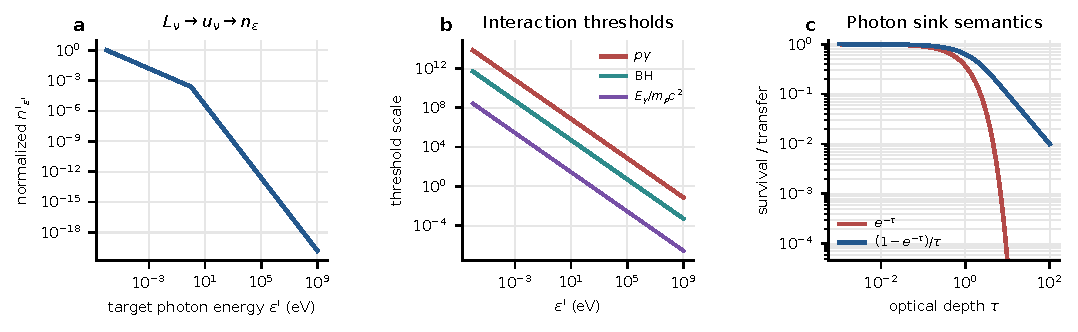
\includegraphics[width=\textwidth]{figures/figA1_hadronic_feedback.pdf}
  \caption{
\gptareaderanchor{gpta-seg-000635}%
强子与对反馈分支记录。(a) 从辐射能量密度转换为光子数密度后的代表性靶光子场。(b) 基于粒子静止质量能量写出的\(p\gamma\)、贝特-海特勒和\(\gamma\gamma\)阈值标度。(c) 纯衰减\(e^{-\tau}\)和有限壳层转移\((1-e^{-\tau})/\tau\)。各面板记录了可选的一维分支；本图未推导出不受支持的\(\chi\)分辨强子输运和IC介导的电磁级联。}
  \label{fig:hadronic-feedback}
\end{figure*}

\section{反向激波技术细节} \label{app:reverse-shock-technical}


\gptareaderanchor{gpta-seg-000636}%
本附录包含了在主要方法部分中过于详细的反向激波代数。它记录了有限强度磁流体力学跳跃、磁化上游记录、事件分裂、穿越后演化、次级密度跳跃激波诊断以及再加速重映射。正文部分保留了喷射物状态、激活边界、跳跃输出、反向电子注入、辐射产物以及支撑边界。

\subsection{有限强度 MHD 跃变三次方程}


\gptareaderanchor{gpta-seg-000637}%
有限强度的MHD跳跃给出了磁化反向激波所使用的下游激波框架四速度。上游状态由相对洛伦兹因子\(g=\gamma_{34}\)和喷出物磁化参数\(\sigma\)来描述。局部代数使用
\begin{equation}
\begin{aligned}
g&\equiv\gamma_{34},\\
\hat{\gamma}&=\frac{4}{3}+\frac{1}{3g},\\
h_1&=\hat{\gamma}-1,\qquad
h_2=\hat{\gamma}-2,\qquad
y&\equiv u_d^2 .
\end{aligned}
\end{equation}

\gptareaderanchor{gpta-seg-000638}%
此处 \(u_d\) 是反向激波参考系中的下游四速度。参数 \(\sigma_{\rm cut}\) 是一个算法分支参数，并非实际的磁化边界。

低 \(\sigma\) 分支返回同一激波参考系问题的流体动力学强度根。
\begin{equation}
y=\frac{(g-1)h_1^2}{-\hat{\gamma}h_2(g-1)+2}.
\end{equation}

\gptareaderanchor{gpta-seg-000639}%
对于 \(\sigma>\sigma_{\rm cut}\)，MHD分支则求解
\begin{equation}
a_3y^3+a_2y^2+a_1y+a_0=0,
\end{equation}
其中
\begin{equation}
\begin{aligned}
a_3={}&-\hat{\gamma}h_2(g-1)+2,\\
a_2={}&-(g+1)\left[-h_2(\hat{\gamma}g^2+1)+\hat{\gamma}h_1g\right]\sigma\\
&-(g-1)\left[-\hat{\gamma}h_2(g^2-2)+2g+3\right],\\
a_1={}&(g+1)\left[\hat{\gamma}\left(1-\frac{\hat{\gamma}}{4}\right)
(g^2-1)+1\right]\sigma^2\\
&+(g^2-1)\left[2g+h_2(\hat{\gamma}g-1)\right]\sigma
+(g+1)(g-1)^2h_1^2,\\
a_0={}&-\frac{1}{4}(g-1)(g+1)^2h_2^2\sigma^2 .
\end{aligned}
\end{equation}

\gptareaderanchor{gpta-seg-000640}%
这些系数体现了跳跃条件中有限的上游磁压和焓。

三次方程通过将其转化为缺项形式来求解。定义
\begin{equation}
\begin{aligned}
b_c&=\frac{a_2}{a_3},\qquad
c_c=\frac{a_1}{a_3},\qquad
d_c=\frac{a_0}{a_3},\\
p_c&=c_c-\frac{b_c^2}{3},\\
q_c&=\frac{2b_c^3}{27}-\frac{b_cc_c}{3}+d_c,\\
a_c&=\left(-\frac{p_c}{3}\right)^{1/2},\\
\psi_c&=\frac{1}{3}\cos^{-1}\!\left(\frac{3q_c}{2p_ca_c}\right).
\end{aligned}
\end{equation}

\gptareaderanchor{gpta-seg-000641}%
壳层动力学所使用的物理根是
\begin{equation}
\begin{aligned}
y&=2a_c\cos\left(\psi_c-\frac{2\pi}{3}\right)-\frac{b_c}{3},\\
u_d&=y^{1/2}.
\end{aligned}
\end{equation}

\gptareaderanchor{gpta-seg-000642}%
那么，上游激波系中的四速度就是
\begin{equation}
u_u=\left[(1+u_d^2)(g^2-1)\right]^{1/2}+g u_d .
\end{equation}

\gptareaderanchor{gpta-seg-000643}%
因此，该跃迁返回了\(u_d\)、压缩比\(r_\sigma=u_u/u_d\)以及初级反向激波状态所使用的磁化下游热量。

\section{投影、拟合与运行时细节} \label{app:projection-runtime}


\gptareaderanchor{gpta-seg-000644}%
本附录记录了支持投影、拟合和可重复性的运行时细节。它给出了等到达时间插值、射线追踪的SSA路径记录、结构化补丁累积、拟合封装器、查询缓存和源数据机制。正文保留了物理投影方程、观测器产品、似然产品、运行时输出和公共边界。

\subsection{前向动力学运行时细节}


\gptareaderanchor{gpta-seg-000645}%
前向动力学运行时记录是一个ABI有序容器。公共模型首先构建一个边界向量，编译后的动力学内核只解包前向激波所需的槽位：
\begin{equation}
\mathbf b_{\rm dyn}\mapsto
\begin{gathered}
\left(
\Gamma_0,\epsilon_e,\epsilon_B,p,z,n_{\rm ISM},A_\ast,E_{\rm iso},
\log_{10}t_{{\rm on},\rm end},f_e
\right),\\
\left(
t_1,t_2,L_0,q,R_{\rm tr},f_{\rm jump},w_{\rm jump},R_0
\right).
\end{gathered}
\end{equation}

\gptareaderanchor{gpta-seg-000646}%
这里 \(t_1, t_2, L_0\) 和 \(q\) 描述可选光度源，而 \(R_{\rm tr}, f_{\rm jump}, w_{\rm jump}\) 和 \(R_0\) 描述解析密度跳跃和内风帽。容器本身并非新的物理模型；它仅规定如何将公共输入传递给编译内核。随后内核从
\begin{equation}
\mathbf{y}_0=(\Gamma_0-\Delta\Gamma_{\rm init},
Y_{2,{\rm init}},U_{\rm init},R_{\rm init}),
\end{equation}

\gptareaderanchor{gpta-seg-000647}%
其中 \(\Delta\Gamma_{\rm init}\), \(Y_{2,{\rm init}}\), \(U_{\rm init}\) 和 \(R_{\rm init}\) 是固定的积分起始参数。这些值在写入按半径排序的激波历史之前设定了第一个数值状态。

前向动力学输出网格建立在源帧的轴上时间坐标上。第一个正网格时间是
\begin{equation}
t_{{\rm on},\min}=\min(t_{\rm floor},\eta_{\rm dec}t_{\rm dec}) ,
\end{equation}

\gptareaderanchor{gpta-seg-000648}%
其中 \(t_{\rm floor}\) 和 \(\eta_{\rm dec}\) 是固定的网格参数。网格和时序更新是
\begin{equation}
\begin{aligned}
\ell_i&=\log_{10}t_{{\rm on},\min}
+\frac{\log_{10}t_{{\rm on},\rm end}
-\log_{10}t_{{\rm on},\min}}{N_R-1}(i-1),\\
t_{{\rm on},i}&=10^{\ell_i},\\
\Delta t_i&=t_{{\rm on},i}-t_{{\rm on},i-1},\qquad t_{{\rm on},0}=0,\\
\mathbf{y}_i&=\mathbf{y}_{i-1}
+\int_{t_{{\rm on},i-1}}^{t_{{\rm on},i}}
F(t_{\rm on},\mathbf{y})\,dt_{\rm on}.
\end{aligned}
\end{equation}

\gptareaderanchor{gpta-seg-000649}%
这里 \(F\) 是从第~\ref{sec:dynamics} 节中选择的正向动力学右侧项。在每次接受的步骤之后，存储的状态是
\begin{equation}
\mathbf{y}_i=(Y_{\Gamma,i},Y_{2,i},Y_{U,i},Y_{R,i}).
\end{equation}

\gptareaderanchor{gpta-seg-000650}%
公共输出数组随后记录 \((1+z)t_{{\rm on},i}\)、\(Y_{\Gamma,i}\)、\(Y_{R,i}\) 以及扫过的质量。演化扫过数柱的分支在写入公共输出之前将其转换为质量。

RK子步变量控制正时间积分区间。它遵循
\begin{equation}
0\le s\le \ln(t_{{\rm on},i}/t_{{\rm on},i-1}),
\qquad
|\Delta s|\le\Delta s_{\max},
\end{equation}

\gptareaderanchor{gpta-seg-000651}%
其中 \(\Delta s_{\max}\) 是一个固定的积分参数。精化过程将试验状态与先前接受的试验进行比较，仅接受动力域 \(\Gamma>1\) 内具有正演化分量的状态。

\section{软件与数据可用性} \label{app:data}


\gptareaderanchor{gpta-seg-000652}%
软件与数据记录界定了本方法论文的证据路径。
\asgard\ 源代码及手稿代码基线由 \citet{ASGARDSoftware} 中的软件记录标识。此处使用的图形证据是 \texttt{paper/source\_data/} 中追踪的源表格。正式图形入口点为 \texttt{tests/generate\_paper\_figures.py}，该文件将绘制的产物写入 \texttt{paper/figures/} 下。这些追踪手稿路径之外的探索性输出不作为论文主张的证据。该实现使用了 NumPy、SciPy、Matplotlib 和 Astropy
\citep{Harris2020,Virtanen2020,Hunter2007,Astropy2022}。

\clearpage

\bibliographystyle{aasjournalv7.1}
\bibliography{references}

\end{document}
